\documentclass[11pt,twoside]{extbook}


%%%%%%%%%%%%%%%%%%%%%%%%%%%%%%%%%%%%%%%%%%%%%%%
            %PACKAGES
%%%%%%%%%%%%%%%%%%%%%%%%%%%%%%%%%%%%%%%%%%%%%%%      

\usepackage[
  %paperwidth=17cm,
  %paperheight=24cm,
  inner=1.8cm,  % margine interno (legatura)
  outer=1.5cm,  % margine esterno
  top=2cm,
  bottom=2cm
]{geometry}
%\usepackage{mathpazo} % Palatino (molto simile a Times ma più leggibile)

\usepackage{subfiles}
\usepackage[italian]{babel}
\usepackage{fontspec}
\setmainfont{Source Sans Pro Light}
\usepackage{latexsym}
\usepackage{amsmath,amsfonts,amssymb,amsthm}
\usepackage{mathtools}
\usepackage{tikz}
\usepackage{microtype} 
\usepackage{graphicx} 
% migliore spezzatura/kerning
\emergencystretch=2em                  % elasticità extra per righe difficili
\raggedbottom 

\usepackage[section]{placeins}
\usepackage{mathdots}
\usepackage{cancel}
\usepackage{color}
\usepackage{siunitx}
\usepackage{array}
\usepackage{multirow}
\usepackage{makecell}
\usepackage{tabularx}
\usepackage{booktabs}
\usepackage{caption}
\usepackage{subcaption}
\usetikzlibrary{fadings}
\usetikzlibrary{patterns}
\usetikzlibrary{shadows.blur}
\usepackage{placeins} % The placeins package gives the command \FloatBarrier, which will make sure any floats will be put in before this point
\usepackage{flafter}  % The flafter package ensures that floats don't appear until after they appear in the code.
\usepackage{bigints}
\usepackage{needspace}
\usepackage{import}
\usepackage{pdfpages}
\usepackage{transparent}
\usepackage{graphicx}
\usepackage{float}
\usepackage{mathrsfs}
\usepackage[none]{hyphenat} % Per non far andare a capo le parole con il trattino
\usepackage[hidelinks]{hyperref} % Rende l'indice interattivo e hidelinks nasconde il bordo rosso dai riferimenti
\usepackage[toc,page]{appendix}
\usepackage{titlesec}
\usepackage{paralist}
\usepackage{enumitem}
\usepackage{pgfplots, tikz}
\usetikzlibrary{trees}
\usetikzlibrary{positioning, calc}
\usepackage{import}
\usepackage{wasysym}
\usepackage{cancel}
\usepackage{fontawesome}
\usetikzlibrary{intersections}
\usepackage{bm}
\usepackage{tikz-3dplot}

\usetikzlibrary{arrows.meta, calc}
\usetikzlibrary{decorations.pathreplacing}
\pgfplotsset{compat=1.18}


\usepackage[dvipsnames]{xcolor}
\usepackage{amsthm}
\usepackage{mathtools}
\usepackage[most]{tcolorbox} 
\allowdisplaybreaks
\tcbset{before skip=7pt, after skip=7pt} % come skipabove/skipbelow
\usepackage{stmaryrd}


% Header e footer in stile libro
\usepackage{fancyhdr}
\pagestyle{fancy}
\fancyhf{} % pulisci

% cosa mostrare in header
\renewcommand{\chaptermark}[1]{\markboth{\thechapter.\ #1}{}}
\renewcommand{\sectionmark}[1]{\markright{\thesection\ #1}}

% header: capitolo a sinistra (pagine pari), sezione a destra (dispari)
\fancyhead[LE]{\small\itshape \nouppercase{\leftmark}}
\fancyhead[RO]{\small\itshape \nouppercase{\rightmark}}

% numero pagina centrato in basso
\fancyfoot[C]{\small\thepage}

% linee
\renewcommand{\headrulewidth}{0.4pt}
\renewcommand{\footrulewidth}{0pt}
\newcommand{\ind}{\mathrel{\perp\!\!\!\perp}}
\newcommand{\verteq}{\rotatebox[origin=c]{90}{$=$}} % uguale verticale

% spaziatura compatta dell'header
\setlength{\headheight}{13.6pt}   % evita warning
\setlength{\headsep}{10pt}        % meno aria sotto l'header




% --- Stile teoremi ------------------------------------------------------------
\makeatletter
\newtheoremstyle{blacknumbox}
  {0pt}{0pt}            % spazio sopra/sotto
  {\normalfont}{}       % corpo normale
  {\bfseries\scshape}   % titolo in small caps
  {:\;}                 % punteggiatura dopo il titolo
  {0.25em}              % spazio dopo il titolo
  {\small
    \thmname{#1}\nobreakspace
    \thmnumber{\@ifnotempty{#1}{\@upn{#2}}}%
    \thmnote{ \normalfont\bfseries\nobreakspace#3 }%
  }
\makeatother

\theoremstyle{blacknumbox}

% --- Contatore master (section per article / chapter per book) ----------------
\makeatletter
\@ifundefined{chapter}
  {\newtheorem{thmT}{Teorema}[section]}
  {\newtheorem{thmT}{Teorema}[chapter]}
\makeatother

% --- Tutti gli ambienti numerati condividono thmT -----------------------------
\newtheorem{definitionT}[thmT]{Definizione}
\newtheorem{NBT}[thmT]{NB}
\newtheorem{propositionT}[thmT]{Proposizione}
\newtheorem{corollarioT}[thmT]{Corollario}
\newtheorem{lemmaT}[thmT]{Lemma}
\newtheorem{teoremaT}[thmT]{Teorema}

% --- Quelli non numerati ------------------------------------------------------
\newtheorem*{ossT}{Osservazione}
\newtheorem*{exT}{Esempio}

% --- Definizione insiemi ------------------------------------------------------
\DeclarePairedDelimiter\set{\{}{\}}
\renewcommand{\set}[1]{\Bigl\{\,#1\,\Bigr\}}

\tcbset{
  bwstyle/.style={
    enhanced, breakable, frame hidden, % niente cornice completa
    borderline west={1pt}{0pt}{black}, % solo linea sinistra nera 1pt
    colback=white, left=5pt, right=5pt, top=5pt, bottom=5pt, boxsep=0pt
  },
  bstyle/.style={
    enhanced, breakable, frame hidden,
    colback=blue!5, left=5pt, right=5pt, top=5pt, bottom=5pt, boxsep=0pt
  },
  ostyle/.style={
    enhanced, breakable, frame hidden,
    borderline west={1pt}{0pt}{orange},
    colback=orange!5, left=5pt, right=5pt, top=5pt, bottom=5pt, boxsep=0pt
  },
  gstyle/.style={
    enhanced, breakable, frame hidden,
    borderline west={2pt}{0pt}{green},
    colback=green!5, left=5pt, right=5pt, top=5pt, bottom=5pt, boxsep=0pt
  }
}


\newenvironment{bwBox}{\begin{tcolorbox}[bwstyle]}{\end{tcolorbox}}
\newenvironment{bBox}{\begin{tcolorbox}[bstyle]}{\end{tcolorbox}}
\newenvironment{oBox}{\begin{tcolorbox}[ostyle]}{\end{tcolorbox}}
\newenvironment{gBox}{\begin{tcolorbox}[gstyle]}{\end{tcolorbox}}


\newenvironment{teorema}{\begin{bwBox}\begin{teoremaT}}{\end{teoremaT}\end{bwBox}}
\newenvironment{proposizione}{\begin{bwBox}\begin{propositionT}}{\end{propositionT}\end{bwBox}}
\newenvironment{definizione}{\begin{bwBox}\begin{definitionT}}{\end{definitionT}\end{bwBox}}
\newenvironment{nb}{\begin{bwBox}\begin{NBT}}{\end{NBT}\end{bwBox}}
\newenvironment{oss}{\begin{bwBox}\begin{ossT}}{\end{ossT}\end{bwBox}}
\newenvironment{corollario}{\begin{bwBox}\begin{corollarioT}}{\end{corollarioT}\end{bwBox}}
\newenvironment{lemma}{\begin{bwBox}\begin{lemmaT}}{\end{lemmaT}\end{bwBox}}
\newenvironment{esempio}{\begin{oBox}\begin{exT}}{\end{exT}\end{oBox}}


% --- dimostrazione annidata e spezzabile ---
\renewcommand{\qedsymbol}{$\square$}
\newenvironment{dimostrazione}
  {\begin{bBox}\begin{proof}[Dimostrazione]}
  {\end{proof}\end{bBox}}


\titleformat{\chapter}[hang]
  {\normalfont\Huge\bfseries} % più grande di Large
  {\thechapter}{1em}{}

\titleformat{\section}
  {\normalfont\Large\bfseries} % da normalsize a Large
  {\thesection}{0.7em}{}

\titleformat{\subsection}
  {\normalfont\normalsize\bfseries} % da small a normali
  {\thesubsection}{0.7em}{}

\titleformat{\subsubsection}
  {\normalfont\small\bfseries} % da footnotesize a small
  {\thesubsubsection}{0.5em}{}


% Spaziature (molto ridotte)
\titlespacing*{\chapter}{0pt}{10pt}{5pt}       % sopra=10pt, sotto=5pt
\titlespacing*{\section}{0pt}{6pt}{3pt}        % sopra=6pt, sotto=3pt
\titlespacing*{\subsection}{0pt}{4pt}{2pt}     % sopra=4pt, sotto=2pt
\titlespacing*{\subsubsection}{0pt}{3pt}{1pt}  % sopra=3pt, sotto=1pt

\newcommand{\ve}[1]{\underline{{\boldsymbol{#1}}}}
% --- Prodotto scalare tra vettori con \ve automatico ---
\newcommand{\scalar}[2]{\left\langle \ve{#1},\, \ve{#2} \right\rangle}
\newcommand{\E}[1]{E\!\left[\,#1\,\right]}
\newcommand{\ex}[1]{%
  \exp\!\left\{#1 \right\}%
}
\newcommand{\nlongrightarrow}{\;\not\!\!\!\longrightarrow}
\newcommand{\nLongrightarrow}{\;\not\!\!\!\Longrightarrow}


\begin{document}
\begin{titlepage}
\newfontfamily\titolofont{Source Sans Pro}
\begin{tikzpicture}[remember picture, overlay]

  % ---- cornice doppia ----
  \draw[line width=1pt]
    ($(current page.north west)+(0.9,-0.9)$) rectangle ($(current page.south east)+(-0.9,0.9)$);
  \draw[line width=0.4pt]
    ($(current page.north west)+(1.08,-1.08)$) rectangle ($(current page.south east)+(-1.08,1.08)$);

  % ---- intestazione ----
  \node[anchor=north] at ($(current page.north)+(0,-2.3)$)
    {\scshape\large Politecnico di Milano};
  \node[anchor=north] at ($(current page.north)+(0,-3.1)$)
    {\itshape Corso di Laurea in Ingegneria Matematica};
  \draw[line width=0.4pt]
    ($(current page.north)+(-2.6,-4.0)$) -- ($(current page.north)+(2.6,-4.0)$);

  % ---- titolo ----
  \node at ($(current page.north)+(0,-8.0)$)
    {\titolofont\fontsize{26}{32}\selectfont\itshape Dispense di};
  \node at ($(current page.north)+(0,-10.3)$)
    {\titolofont\fontsize{50}{60}\selectfont\bfseries\scshape Probabilità};

  % ---- istogramma che converge alla gaussiana ----
  \begin{scope}[shift={($(current page.north)+(0,-19.6)$)}, xscale=1.35, yscale=4.6]
    \foreach \x/\h in {-3.25/0.02, -2.75/0.03, -2.25/0.10, -1.75/0.19,
                       -1.25/0.49, -0.75/0.72, -0.25/1.00, 0.25/0.95,
                        0.75/0.78, 1.25/0.44, 1.75/0.23, 2.25/0.07,
                        2.75/0.03, 3.25/0.015}
      \draw[fill=RoyalBlue!12, draw=RoyalBlue!60, line width=0.3pt]
        (\x-0.235,0) rectangle (\x+0.235,\h);
    \draw[orange, dashed, line width=0.8pt] (0,0) -- (0,1.08);
    \node[orange, above] at (0,1.08) {\small $\mu$};
    \draw[line width=1.1pt, smooth, domain=-3.6:3.6, samples=120]
      plot (\x, {exp(-\x*\x/2)});
    \draw[line width=0.6pt] (-3.95,0) -- (3.95,0);
  \end{scope}

  \node at ($(current page.north)+(0,-21.1)$)
    {\color{gray}$\displaystyle \varphi(x)=\frac{1}{\sqrt{2\pi}}\,e^{-x^2/2}$};

  % ---- autore ----
  \draw[line width=0.4pt]
    ($(current page.south)+(-2.6,4.6)$) -- ($(current page.south)+(2.6,4.6)$);
  \node at ($(current page.south)+(0,3.7)$)
    {\Large\scshape Marco Zamboni};
  \node at ($(current page.south)+(0,2.9)$)
    {A.A. 2024/2025};

\end{tikzpicture}
\null
\end{titlepage}

\let\cleardoublepage\clearpage 

\tableofcontents

\part{Teoria}
\mainmatter
\chapter{Cenni di Teoria della Misura}
\section{Sigma--Algebra}
Definito $\Omega$ come un insieme, di questo ci interessano famiglie di sottoinsiemi. Per esempio possiamo avere l'Insieme delle Parti di $\Omega$, ovvero l'insieme che contiene tutti gli insiemi di $\Omega$. 
    \[\mathcal{P}(\Omega) = 2^\Omega = \{A: A\subseteq \Omega\}\]

\begin{esempio}
Insieme delle parti di $\Omega = \{0, 1\}$: \[\mathcal{P}(\{0, 1\}) =\{\{0\}, \{1\}, \{0, 1\}, \varnothing\}\]
Oppure possiamo considerare famiglie di sottoinsiemi differenti di $\Omega = \mathbb{R}$, per esempio:
\begin{itemize}
    \item $\{\mathbb{N}\}$
    \item $\set{(a, b): -\infty < a < b < \infty}$ \hfill \textit{(Tutti gli intervalli aperti)}
    \item $\set{\varnothing, (a, b): -\infty < a < b < \infty}$
\end{itemize}
\end{esempio}
Una caratteristica fondamentale che devono avere queste sottofamiglie, è che siano $\sigma$--Algebre.
\begin{definizione}
    $\mathcal{A} \subseteq \mathcal{P}(\Omega)$, famiglia di sottoinsiemi di $\Omega$, è una $\sigma$--algebra se:
    \begin{enumerate}
    \item $\Omega \in \mathcal{A}$ 
    \item Se $A \in \mathcal{A} \;\Rightarrow\; A^c \in \mathcal{A}$ \hfill \textit{(chiusa al passaggio per complementare)}
    \item $A_1, ..., A_n \in \mathcal{A} \;\Rightarrow\;$ $\bigcup_{k=1}^{n} A_k \in \mathcal{A}$ \hfill \textit{(chiusa rispetto all'unione finita)}
    \item $(A_n: \; n \geq 1) \subseteq \mathcal{A} \;\Rightarrow\; \bigcup_{n=1}^{\infty} A_n \in \mathcal{A}$ \hfill \textit{(chiusa rispetto unione numerabile)}
\end{enumerate}
\end{definizione}

\begin{esempio}
    Alcuni esempi possono di sigma algebre di $\Omega = \{0, 1\}$ possono essere:
    \begin{itemize}
        \item $\set{\varnothing, \{0\}, \{1\}, \{0, 1\}}$
        \item $\set{\varnothing, \{0, 1\}}$
        \item $\set{\varnothing, \mathbb{R}}$ \hfill \textit{($\sigma$--algebra banale)}
        \item $\set{\varnothing, \mathbb{R}, (-\infty, 0], (0, +\infty)}$
    \end{itemize}
Mentre se prendiamo $\set{ \varnothing, \{[a, b): -\infty < a < b < \infty\}}$, questa non risulta essere una sigma--algebra, in quanto possiamo prendere l'intervallo $[1, 2)$, il quale ha come complementare $[1, 2)^c = (-\infty, 1) \cup [2, \infty)$, il quale non si riesce a scrivere come intervallo del tipo $[a, b): -\infty < a < b < \infty$.
\end{esempio}
Si noti che il punto 4 della definizione di $\sigma$--algebra è pleonastico. Questo deriva dalle regole di De Morgan, che ricordiamo essere (su famiglie finite e numerabili):

\begin{center}
$\left( \bigcup_\alpha A_\alpha \right)^c = \bigcap A_\alpha^c$ 
\quad \quad e \quad \quad
$\left( \bigcap_\alpha A_\alpha \right)^c = \bigcup A_\alpha^c$
\end{center}
Si ha dunque che se: \\
\[A_1 ,..., A_n \in \mathcal{A} \xRightarrow{(2)} A_1^c ,..., A_n^c \in \mathcal{A}\xRightarrow{(3)} \bigcup_{k=1}^n A_k^c \in \mathcal{A} \xRightarrow{(2)} \left(\bigcup_{k=1}^n A_k^c \right)^c \in \mathcal{A} \overset{(D.M.)}{=} \bigcap_{k=1}^\infty A_k\]
Possiamo quindi andare a ripulire la definizione stessa, attraverso la seguente proposizione:

\begin{proposizione}
    Se per una classe $\mathcal{C}$ di sottoinsiemi di $\Omega$ vale che:
    \begin{enumerate}
        \item $\Omega \in \mathcal{C}$
        \item $A \in \mathcal{C} \Rightarrow A^c \in \mathcal{C}$
        \item $(A_n)_{n\geq1} \subseteq \mathcal{C} \Rightarrow \bigcup_{n=1}^\infty \in \mathcal{C}$
    \end{enumerate}
        Allora se $A_1, ..., A_n \in \mathcal{C}$ anche $\bigcup_{k=1}^{n} A_k \in \mathcal{C}$.
\begin{dimostrazione}
    Sapendo che valgono 1. 2. e 3. e che vale che $\varnothing \in \mathcal{C}$ mi costruisco una successione numerabile $\in \mathcal{C}$:
    \[(B_k)_{k\geq1} \subseteq \mathcal{C}: 
    \begin{cases} 
    B_k = A_k, & \text{se } 1\leq k\leq n \\ 
    B_k = \varnothing, & \text{se } k \geq n+1
    \end{cases}
\]
Allora: \[\bigcup_{k=1}^{\infty} B_k \in \mathcal{C} \;\;\; \Rightarrow \;\;\; \bigcup_{k=1}^{\infty} B_k = A_1 \cup ...\cup A_n \cup \varnothing  \cup ...\cup \varnothing  = A_1 \cup ... \cup A_n\]
\end{dimostrazione}
\end{proposizione}
Possiamo quindi finalmente ripulire la definizione di $\sigma$--algebra alla luce della proposizione 1.2:

\begin{definizione}
    $\mathcal{A} \subseteq \mathcal{P}(\Omega)$ famiglia di sottoinsiemi di $\Omega$ è una $\sigma-algebra$ se: 
\begin{enumerate}
    \item $\Omega \in \mathcal{A}$ 
    \item Se $A \in \mathcal{A} \;\Rightarrow\; A^c \in \mathcal{A}$ 
    \item $(A_n)_{n \geq 1} \subseteq \mathcal{A} \;\Rightarrow\; \bigcup_{n=1}^{\infty} A_n \in \mathcal{A}$ 
\end{enumerate}
\end{definizione}
Questo implica che se $\mathcal{A}$ è una $\sigma$-- algebra, questa è chiusa anche ad unioni finite e ad intersezioni finite e numerabili.\\

\section{Misure e Spazi Misurabili}
Uno spazio misurabile $(\Omega, \mathcal{A})$ è una coppia formata da un insieme $\Omega$ ed una $\sigma$--algebra $\mathcal{A}$ di sottoinsiemi. Osserviamo che si possono sempre trovare $\sigma$--algebre banali, come $\mathcal{A} = \{\varnothing, \Omega\}$ oppure $\mathcal{A} = \mathcal{P}(\Omega) = 2^\Omega$. O addirittura possiamo costruire una $\sigma$--algebra a partire da un sottoinsieme:
\[A\subseteq \Omega \quad \rightarrow \quad \mathcal{A} = \sigma (A) = \set{\varnothing, \Omega, A, A^c}\]

\begin{definizione}
    Una Misura $\mu$ su $\mathscr{E}$ è una funzione $\mu:\mathscr{E}\rightarrow \mathbb{R}^+ \cup\{+ \infty\}$ tale che:
    \begin{itemize}
        \item [M.1)] $\mu(\varnothing) = 0$
        \item [M.2)] Vale la $\sigma$--additività, ovvero che:\\
        $(E_n)_{n \geq 1} \subseteq \mathscr{E}$ tale che $E_h \cap E_k = \varnothing \;\;\; \forall k \neq h: \;\; \mu(\bigcup_{n=1}^{\infty} E_n) = \sum_{n=1}^{\infty}\mu(E_n)$ 
    \end{itemize}
\end{definizione}

\begin{definizione}
    $\mu$ è una misura finita se $\mu(E) < +\infty$
\end{definizione}

\begin{definizione}
\label{def:sigmafinita}
    $\mu$ è una misura $\sigma$--finita se $\exists (E_n)_{n \geq 1} \subseteq \mathscr{E}$ tale che:
    \begin{enumerate}
        \item $E=\bigcup_{n=1}^{\infty} E_n$
        \item $\mu(E_n) < + \infty\;\;\;\forall n \geq1$
    \end{enumerate}
\end{definizione}

Si osservi che in quest'ultima definizione non abbiamo imposto alcuna restrizione sul fatto che gli insiemi vadano presi a due a due disgiunti; nel caso siano anche disgiunti, non abbiamo sicurezza che la serie sia finita. Notiamo inoltre che la misura di $E$ non deve essere per forza finita per essere $\sigma$--finita; l'essere $\sigma$--finiti è un caso più generale dell'essere finiti.

\begin{esempio}
    Misura di Lebesgue\\
    $E = \mathbb{R}\quad;\quad\mu=m\quad$ dove:
    \[m([a, b))= b-a= \int_a^bdx\] 
    Ovvero associo ad un intervallo la sua lunghezza. Mi aspetto quindi che "$m(\mathbb{R}) = +\infty$" ossia che la "\textit{misura della retta reale si infinita}". Se notiamo che possiamo scrivere $\mathbb{R}$ come: 
    \[\mathbb{R} = \bigcup_{n=1}^\infty [-n, n) = \bigcup_{n=1}^\infty E_n\]
    e che $m([-n, n)) = 2n \quad \Rightarrow \quad \mu (E_n) = m([-n, n)) = 2n < +\infty$.\\
    Abbiamo quindi dimostrato che la Misura di Lebesgue è $\sigma$--finita.\\
    Osservo che $\mathbb{R}^+$ può essere scritto come unione \emph{disgiunta} di intervalli a misura finita:
    \[
    \mathbb{R}^+ = \bigcup_{n=0}^{\infty} [n, n+1),
    \]
    dove $\;[n,n+1) \cap [k,k+1) = \varnothing \quad \forall n \neq k$.\\
    Inoltre
    \[
    \mu([n,n+1)) = 1 < +\infty \qquad \forall n \in \mathbb{N},
    \]
quindi $\mu$ è $\sigma$-finita anche su $\mathbb{R}^+$.
\end{esempio}

\begin{proposizione}
    Sia $\mu$ una misura su $(E, \mathscr{E})$, allora valgono le seguenti proprietà:
    \begin{enumerate}
        \item [P.1)] $\mu(A\cup B) = \mu(A) + \mu(B)\;\;\;\forall A\cap B = \varnothing\;\;\;A, B \in \mathscr{E}$
        \item [P.2)] $\mu(A) \leq \mu(B)$ quando $A\subseteq B$
    \end{enumerate}
    
    \begin{dimostrazione}
    $A, B \in \mathscr{E}$ e posso scrivere che $A \cup B = A \cup B \cup \varnothing  \cup ...\cup \varnothing = \bigcup_{n=1}^\infty E_n$, dove:
    \[
    E_n =
    \begin{cases}
        E_1 = A & \\
        E_2 = B & \\
        E_3 = \varnothing, & \text{se } k \geq 3
    \end{cases}
    \]
    \begin{itemize}
        \item [P.1)] $\mu(A \cup B) = \mu(\bigcup_{n=1}^\infty E_n) \overset{\text{M.2}}{=} \sum_{n\geq1} \mu(E_n) = \mu(E_1) + \mu(E_2) + \sum_{n\geq3} \mu(E_n) = \mu(A) + \mu(B) + \sum_{n\geq3} 0 = \mu(A) + \mu(B)$
        \item [P.2)]  Partiziono B come: $B = A \cup (B \cap A^c)$, la quale è unione disgiunta $(A \cap (B \cap A^c)) = \varnothing$.
        \begin{center}
            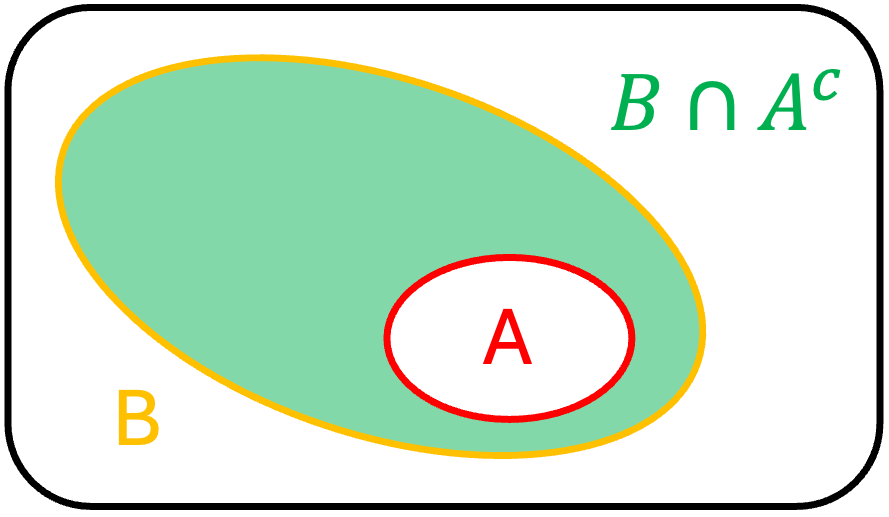
\includegraphics[width=0.2\textwidth]{Media/Dim_1.7.png}
        \end{center}
        $\overset{\text{P.1}}{\Rightarrow}\;\;\; \mu(B) = \mu(A \cup (B \cap A^c)) = \mu(A) + \mu(B \cap A^c)) \geq \mu(A)$ \\
        In quanto la misura è non negativa.
    \end{itemize}
    
    \end{dimostrazione}
\end{proposizione}

\vspace{\baselineskip}
\subsection{Alcune misure fondamentali}
\begin{itemize}[label=\(\bigstar\), align=left, labelsep=0.5em, labelwidth=!, leftmargin=0pt]
\item Una misura fondamentale nella Teoria della misura è la \textbf{Massa di Dirac} in un punto $\alpha_0$.\\
Preso  $\alpha_0 \in E$, si ha che $\forall A \subseteq E$:
\[ \mu(A) = 
\begin{cases} 
    1, & \text{se } \alpha_0 \in A \\ 
    0, & \text{se } \alpha_0 \notin A
\end{cases}
\]
Questa risulta essere una misura finita.\\
Se infatti prendo $E = \mathbb{R};\alpha_0 = 0;A = [-3, 5)\quad \Rightarrow \quad \mu(A) = 1$\\
Se prendessi invece $B = [-3, -1)\quad \Rightarrow \quad \mu(B) = 0$.\\
Notiamo inoltre che se scrivessi $\mathbb{R}$ come fatto nell'esempio della misura di Lebesgue, non avrei insiemi disgiunti, e di conseguenza non potrei dire che $\mathbb{R}$ ha misura infinita.
\item Consideriamo adesso un'altra misura: la \textbf{Misura Puramente Atomica}. Preso $E$ numerabile, ovvero: $E = \set{\alpha_n : n\geq 0}$, associo a $(\alpha_n)_n$ un'altra successione $(p_n)_{n\geq 0}$ tale che $p_n\geq0$. Siccome $E$ è misurabile avremo che \[A = \bigcup_{k:\alpha_k\in A}\{\alpha_k\}\]
Posso quindi definire la misura:
\[\mu(A) = \sum_{k:\alpha_k\in A} p_k\]
È come se si vedono gli elementi della successione che sono in $A$, e ne sommo i relativi pesi $p_k$; essendo quest'ultimi non negativi la serie non dipenderà dall'ordine, quindi avremo o convergenza o divergenza.
\newpage
\begin{esempio}
    Caso finito.\\
    \[E  = \{1, ..., 6\} \xrightarrow{Associo} \left(\frac{1}{6}, \frac{1}{6}, \frac{1}{6}, \frac{1}{6}, \frac{1}{6}, \frac{1}{6}\right)
    \]
    \[\{\alpha_1, ..., \alpha_6\} \xrightarrow{Associo} (p_1, ..., p_6)\]
    Sia $A\subseteq E: A = \{2, 4, 6\}$\\
    \[\Rightarrow \mu(A) = \sum_{k:\alpha_k\in A} p_k = p_2 + p_3 + p_6 = \frac{1}{6} + \frac{1}{6} + \frac{1}{6} = \frac{1}{2} \]
    Questo caso risulta parecchio semplificato perché l'insieme è finito.
\end{esempio}

\begin{esempio}
    Caso Numerabile.\\
    \[E = \mathbb{N}^* = \mathbb{N} \setminus\{0\} = \{\alpha_n : n\geq 1\} = \{n : n\geq 1\} \xrightarrow{Associo} p_n = n \quad \forall n\geq1\]
    Sia $A\subseteq E$, tale che $A = \{n_k:k\geq1\}$, ovvero che sia una sotto-successione. La misura in questione risulta essere quindi:
    \[\mu(A) = \sum_{k=1}^\infty p_k = \sum_{k=1}^\infty \frac{1}{n_k}\]
    La quale diverge se la si calcola in $E$, rendendo la misura \textit{non} finita:
    \[\mu(E) = \sum_{n=1}^\infty p_n = \sum_{n=1}^\infty \frac{1}{n} = +\infty\]
    Tuttavia si può partizionare l'insieme $E$, andando ad identificare gli insiemi $E_k = \{k\}$, avendo così che $\mu(E_k) = 1/k < +\infty\quad \forall k \geq 1$.\\
    Se inoltre ci si accorge che \[\bigcup_{k\geq1} E_k = \bigcup \{k\} = \mathbb{N}^* = E\]
    allora si può concludere che $\mu$ sia una misura $\sigma$-finita.\\
    \\
    Questo esempio dimostra un fatto fondamentale: se ho una successione numerabile, posso sempre invadere l'insieme nella modalità appena eseguita, verificando sempre che $\mu$ sia una misura $\sigma$-finita.
\end{esempio}

Si noti che preso $E = \{\alpha_n:n\geq1\}$, ovvero un insieme numerabile, e $(p_n)_{n\geq1}:\quad p_n\geq0\quad \forall A\in\mathcal{P}(E)$, allora si avrà sempre che
\[\mu(A) = \sum_{k:\alpha_k\in A} p_k\]
e di conseguenza, si avrà che: \(\mu(E) = \sum_{n} p_n\) dimostrando che
\(\mu \text{ è finita} \iff \sum_{n} p_n < +\infty\).\\
\\
Si noti inoltre che possiamo scrivere la misura come:
\[\mu(A) = \sum_{k:\alpha_k\in A} p_k = \sum_{n=1}^\infty p_n \cdot \delta_{\alpha_n}(A)\]
ossia che possiamo vederla come una \textit{combinazione lineare} di masse di Dirac.

\item La \textbf{Misura di Lebesgue} è già stata introdotta, tuttavia questa può essere estesa anche a casi non monodimensionali. Si ha infatti che:
\begin{enumerate}
    \item Su $\mathbb{R}:\qquad \;\,m_1([a, b)) = b-a$ \hfill \textit{(Lunghezza)}
    \item Su $\mathbb{R}^2:\qquad m_2(B(0, r)) = \pi r^2$ \hfill \textit{(Area)}
    \item Su $\mathbb{R}^3:\qquad m_2(B(0, r)) = \frac{4}{3}\pi r^3$ \hfill \textit{(Volume)}
\end{enumerate}
Anticipiamo che $m$ non può essere definita su tutti i sottoinsiemi di $\mathbb{R}$ perché sono "troppi"; non potremo quindi usare come $\sigma$-algebra $\mathcal{P}(\mathbb{R})$. Più avanti approfondiremo la questione, andando ad individuare una $\sigma$-algebra che sia adatta ai nostri scopi.
\end{itemize}

\chapter{Cosa vuol dire \textit{Probabilità}?}

\section{Terna di Kolmogorov}
Per capire cosa voglia dire \textit{Probabilità}, dobbiamo prima capire dove \textit{si può fare Probabilità}. Introduciamo quindi la Terna Assiomatica della Probabilità (o di Kolmogorov). Un modello probabilistico è quindi un oggetto matematico, composto da tre elementi:
\[(\Omega, \mathcal{A}, \mathbb{P})\]
Dove abbiamo già visto che $(\Omega, \mathcal{A})$ è uno spazio misurabile, ma cosa è $\mathbb{P}$?\\
Andiamo a studiare tutti e 3 gli elementi nel dettaglio.\\
\\
Lo \textbf{Spazio Campionario} $\Omega$ è l'insieme che contiene tutti i possibili risultati del fenomeno (o esperimento) aleatorio che ci interessa. Tutti gli elementi di $\Omega$ sono denotati da $\omega \in \Omega$ dove $\omega$ è definito \textit{risultato} o \textit{realizzazione} dell'esperimento.

\begin{esempio}
Di seguito alcuni esempi su come si può costruire lo spazio campionario:
\begin{enumerate}
    \item  Se lancio una moneta e guardo che faccia esce, lo spazio:
    campionario può essere \[\Omega = \{t, c\} = \{1, 0\}\]
    \item Se lancio 2 monete in successione invece potrei avere: 
    \[\Omega = \set{(t, t), (t, c), (c, t), (c, c)} = \set{0, 1} \times \set{0, 1}\]
    \item Lancio due monete e voglio considerare il numero di teste:
    \[\Omega_1 = \{0, 1, 2\} \quad \text{oppure} \quad \Omega_2 = \set{0, 1} \times \set{0, 1}\] 
    Entrambi gli spazi campionari mi danno lo stesso numero di informazioni sul numero di teste; vanno bene entrambi allo stesso modo per rappresentare l'esperimento.
    \item Accendo una lampadina ed osservo quando si spegne:
    \[\Omega_1 = \mathbb{R}^+ = [0, +\infty) \quad \text{oppure} \quad \Omega_2 = [0, 2T^*]\]
    $\;T^*$ rappresenta la vita massima della lampadina (ammesso che ne siamo a conoscenza).
\end{enumerate}
\end{esempio}
Già da questi banali esempi abbiamo capito che $\Omega$ non è univoco: dipende dall'esperimento\footnote{Ove possibile, è sempre meglio scegliere $\Omega \subseteq \mathbb{R}$ oppure $\Omega \subseteq \mathbb{R}^n$}.\\
\\
La \textbf{Sigma-Algebra} $\mathcal{A}$ è la famiglia degli eventi relativi all'esperimento aleatorio di cui si è interessati a calcolarne la probabilità (anche se non sappiamo ancora cos'è una probabilità). Indichiamo con \textit{Evento} una proposizione logica che so se è vera o falsa \textit{dopo} che ho svolto l'esperimento aleatorio.
\[\text{Evento} \xleftrightarrow{Corrisponde} \text{Sottoinsieme di }\Omega \text{ formato dai risultati che realizzano l'evento stesso}\]

\begin{esempio}
    Riprendendo gli esempi di prima:
    \begin{enumerate}
        \item Se lancio il dado e vedo cosa esce, potrei avere $\Omega = \{1, 2, 3, 4, 5, 6\}$. Un evento potrebbe essere \textit{"lancio il dado ed esce un numero pari"}, che può essere rappresentato dal sottoinsieme $A \subseteq \Omega: A = \{2, 4, 6\}$.\\
        Se effettivamente esce un numero pari (es. 2): $2\in A \Rightarrow A \text{ si è realizzato}$\\
        Se effettivamente esce un numero dispari (es. 3): $3\notin A \Rightarrow A^c \text{ si è realizzato}$
        \item Se lancio due volte una moneta e considero l'evento \textit{$A$ = "esce testa al primo lancio"}, avremo che $\Omega = \{0, 1\} \times\{0, 1\} = \set{(0,0), (0,1), (1, 0), (1, 1)}$ e quindi $A = \set{(1, 0), (1, 1)}$
        \item Osservo una lampadina e segno quando questa muore, allora avremo che $\Omega = [0, +\infty)$. Se si considera l'evento \textit{$A = $"La lampadina dopo 2 ore è ancora accesa"} si avrà che $A = (2, +\infty)$
    \end{enumerate}
\end{esempio}
\bigskip
\noindent Ma come mai c'è la necessità modellistica che $\mathcal{A}$ debba per forza essere una $\sigma$-algebra?\\
\\
Se prendiamo in considerazione un esperimento dove si lancia ripetutamente una moneta, e considero l'evento
\(A_n = \textit{"all'ennesimo lancio esce testa per la prima volta"}\), allora possiamo prendere
\[\Omega = \set{(0, 0, 0,0, 1, 0, 1, ...), ...,...} = \set{(a_n)_{n\geq1}: a_n \in \{0, 1\} \quad \forall n\geq1}\]
\[\Rightarrow A_{\overline{n}} = \set{(a_k)_{k\geq1}: a_h = 0\quad \forall h = 1, ..., \overline{n}-1;\quad a_{\overline{n}}=1} \qquad \text{con } \overline{n} \text{ fissato}\]
Se invece considerassimo l'evento $B = \textit{"Prima o poi esce testa"}$, siamo costretti a modellizzarlo come
\[B = \set{(\mathbf{0})}^c = \bigcup_{n=1}^\infty A_n\]
La quale è un'unione numerabile di eventi: ecco che compare la necessità che la nostra famiglia di eventi $\mathcal{A}$ sia chiusa rispetto all'unione numerabile, e quindi che sia una $\sigma$-algebra.\\
Per completezza diamo anche la definizione di Algebra.
\begin{definizione}
     Una famiglia $\mathcal{A}_0$ di sottoinsiemi di $\Omega$ si definisce algebra se valgono:
    \begin{enumerate}
        \item $\Omega \in \mathcal{A}_0$ 
    \item Se $A \in \mathcal{A}_0 \;\Rightarrow\; A^c \in \mathcal{A}_0$
    \item $A_1, ..., A_n \in \mathcal{A}_0\;\;\; \Rightarrow \;\;\; \bigcup_{k=1}^{n} A_k \in \mathcal{A}_0$
    \end{enumerate}
\end{definizione}
È evidente che una $\sigma$-algebra risulta essere un'algebra, ma non vale il viceversa

\section{La Probabilità}
Finalmente ora abbiamo tutti gli strumenti necessari per dare la definizione formale di cosa sia una probabilità.
\begin{definizione}
    Sia $(\Omega, \mathcal{A})$ uno spazio misurabile (o probabilizzabile). Una probabilità $\mathbb{P}$ è una misura finita su $\mathcal{A}$ tale che $\mathbb{P}(\Omega)=1$, ovvero che:
    \begin{enumerate}
        \item $\mathbb{P}(\varnothing)=0$
        \item $\forall(A_n)_{n\geq1}\subseteq\mathcal{A}$ successione di eventi incompatibili a 2 a 2 (ossia: $A_h \cap A_k = \varnothing\;\;\;\forall h \neq k$) si ha che : \[\mathbb{P}\left(\bigcup_{n=1}^{\infty} A_n\right) = \sum_{n=1}^{\infty}\mathbb{P}(A_n)\]
        \item $\mathbb{P}(\Omega)=1$
    \end{enumerate}
\end{definizione}

Si osservi che la condizione 2. vale solo per famiglie numerabili. Anticipando un concetto che esploreremo più avanti, se questa valesse anche per famiglie più che numerabili, otterrei un assurdo:
\[\Omega = [0, 1] = \bigcup_{x\in[0, 1]}\{x\}\qquad \rightarrow\qquad 1 = \mathbb{P}([0, 1]) \neq \sum_{x\in [0, 1]} \mathbb{P}(\{x\}) = 0 \]
In quanto la probabilità di un atomo $\{x\}$ è zero: $\mathbb{P}(\{x\}) = 0 \quad \forall x \in [0, 1]$

\begin{proposizione}
    Se $\mathbb{P}:\mathcal{A}\rightarrow\mathbb{R}^+ \cup \{+\infty\}$ tale che valgono:
    \begin{itemize}
        \item [(a)] $\mathbb{P}(\Omega)=1$
        \item [(b)] vale la $\sigma$--additività
    \end{itemize}
    Allora $\mathbb{P}(\varnothing)=0$ e quindi la funzione $\mathbb{P}$ è una misura di probabilità (o probabilità).\\
    \begin{dimostrazione}
        Posso scrivere che $\Omega = \Omega \cup \varnothing\cup...\varnothing \cup... = \bigcup_n A_n$, con:
        \[
        A_n = 
    \begin{cases}
        A_1 = \Omega & \\
        A_k = \varnothing, & \text{se } k \geq 2
    \end{cases}
        \]
    Allora:
    \[
    1 \overset{\text{a}}{=} \mathbb{P}(\Omega)
    \overset{\text{b}}{=} \sum_{n=1}^{\infty} \mathbb{P}(A_n) 
    = \mathbb{P}(A_1) + \sum_{n=2}^{\infty} \mathbb{P}(A_n)
    = \mathbb{P}(\Omega) + \sum_{n=2}^{\infty} \mathbb{P}(\varnothing)
    = 1 + \sum_{n=2}^{\infty} \mathbb{P}(\varnothing)\]
\[\;\Rightarrow\;
\sum_{n=2}^{\infty} \mathbb{P}(\varnothing) = 0
\]

\[
\Rightarrow\;\; \mathbb{P}(\varnothing) = 0
\]
Siccome $\mathbb{P}()$ è non negativa.
    \end{dimostrazione}
\end{proposizione}
Come avevamo ripulito la definizione di $\sigma$-algebra, grazie a questa proposizione possiamo ripulire la definizione di Probabilità:
\begin{definizione}
    Una funzione $\mathbb{P}:\mathcal{A}\rightarrow\mathbb{R}^+ \cup \{+\infty\}$ tale che valgono:
    \begin{itemize}
        \item [(a)] $\mathbb{P}(\Omega)=1$
        \item [(b)] vale la $\sigma$--additività
    \end{itemize}
    È una Probabilità su $\mathcal{A}$ (o misura di probabilità).
\end{definizione}

\begin{teorema}[ Proprietà Di Una Probabilità]
    Se $\mathbb{P}$ è una Probabilità su $(\Omega, \mathcal{A})$ allora valgono le seguenti proprietà:
    \begin{enumerate}
        \item [P.1)] $\mathbb{P}(\varnothing)=0$
        \item [P.2)] $A_1, ...,A_n \in \mathcal{A}:\;\;\; A_h\cap A_k \neq\varnothing, \;\;\; \forall h\neq k$ si ha che:\hfill \textit{(finita additività)}
        \[\mathbb{P}(A_1\cup ...\cup A_n)= \sum_{k=1}^{n}\mathbb{P}(A_k)\] 
        \item [P.3)] $A, A' \in \mathcal{A}$ e $A \subseteq A'\;\;\; \Rightarrow \;\;\; \mathbb{P}(A) \leq \mathbb{P}(A')$ 
        \item [P.4)] $\mathbb{P}(A^c) = 1- \mathbb{P}(A)$
        \item [P.5)] $A, A': \;\;\; A'\setminus A = A' \cap A^c \;\;\; \Rightarrow \;\;\; \mathbb{P}(A'\setminus A) = \mathbb{P}(A') - \mathbb{P}(A \cap A')$
        \item [P.6)] $A, A'\in \mathcal{A}: \;\;\; \mathbb{P}(A\cup A') = \mathbb{P}(A)+\mathbb{P}(A')-\mathbb{P}(A\cap A')$
        \item [P.7)] $A_1, ...,A_n \in \mathcal{A}:$ \hfill \textit{(sub--additività)}\[\mathbb{P}(A_1\cup ...\cup A_n)\leq \sum_{k=1}^{n}\mathbb{P}(A_k)\]
        \item [P.8)] $(A_n)_{n\geq 1} \subseteq\ \mathcal{A}:$ \hfill ($\sigma$--sub--additività)
        \[\mathbb{P}(\bigcup_{n=1}^{\infty}A_n)\leq \sum_{n=1}^{\infty}\mathbb{P}(A_n)\]
        \item [P.9)] $A_1, ...,A_n \in \mathcal{A}:$ \hfill \textit{(disguaglianza di Bonferroni)}
        \[\mathbb{P}(A_1 \cap ... \cap A_n) \geq \mathbb{P}(A_1)+...+ \mathbb{P}(A_n)-(n-1)\]
    \end{enumerate}
\end{teorema}
\noindent
\begin{dimostrazione}
    \begin{itemize}
        \item [P.1)] Dimostrata con Proposizione 4.2
        \item [P.2)] Dimostrata in generale per le misure: 1.7 P.1)
        \item [P.3)] Dimostrata in generale per le misure: 1.7 P.2)
        \item [P.4)] Posso partizionare $\Omega$ come $\Omega = A\cup A^c$, che è un'unione disgiunta per definizione.
        \[1\overset{\text{a}}{=}\mathbb{P}(\Omega) = \mathbb{P}(A)+\mathbb{P}(A^c) \;\;\; \Rightarrow \;\;\;\mathbb{P}(A^c) = 1-\mathbb{P}(\Omega)\]
        \item [P.5)] $A, A': \;\;\; A'\setminus A = A' \cap A^c$. Partiziono: $A' = (A'\cap A)\cup (A'\cap A^c)$, che è unione disgiunta.
        \[\Rightarrow\;\;\; \mathbb{P}(A') = \mathbb{P}(A'\cap A) + \mathbb{P}(A'\setminus A)\]
        
        \item [P.6)] \(A\cup B = (A \setminus B)\cup(B\setminus A)\cup (A\cap B)\)
        \begin{align*}
            \Rightarrow\;\;\; \mathbb{P}(A \cup B) &= \mathbb{P}(A \setminus B) + \mathbb{P}(B\setminus A) +\mathbb{P}(A\cap B) \\ &= \mathbb{P}(A) -\mathbb{P}(A\cap B) + \mathbb{P}(B) - \mathbb{P}(A \cap B) + \mathbb{P}(A \cap B)\\ & = \mathbb{P}(A) + \mathbb{P}(B)-\mathbb{P}(A\cap B)
        \end{align*}
        
        \item [P.7)] Dimostro per induzione.\\
        \begin{itemize}
            \item n=2:
            \[\mathbb{P}(A_1 \cup A_2) \overset{\text{P.6}}{=} \mathbb{P}(A_1) + \mathbb{P}(A_2)-\mathbb{P}(A_1\cap A_2) \leq \mathbb{P}(A_1) + \mathbb{P}(A_2) \]
            \item Suppongo vera per n-1, dimostro per n:
            \(A_1 \cup...\cup A_n = (A_1 \cup ... \cup A_{n-1}) \cup A_n\)
            \begin{align*}
                \Rightarrow\;\;\; \mathbb{P}(A_1 \cup...\cup A_n) 
                &\overset{\text{n=2}}{\leq} \mathbb{P}(A_1 \cup ... \cup A_{n-1}) + \mathbb{P}(A_n) \\
                & \overset{\text{n-1}}{\leq} \mathbb{P}(A_1) + ... + \mathbb{P}(A_{n-1}) + \mathbb{P}(A_n)
            \end{align*}
        \end{itemize}
        \item [P.8)] Non la dimostriamo \footnote{Per i più curiosi, potrà essere successivamente dimostrata grazie al Teorema 2.6}
        \item [P.9)] Per induzione:
        \begin{itemize}
            \item n=2: \(\mathbb{P}(A_1 \cap A_2) \overset{\text{P.6}}{=} \mathbb{P}(A_1) + \mathbb{P}(A_2) - \mathbb{P}(A_1 \cup A_2)\)\\
            Dove so che $0 \leq \mathbb{P}(A)\leq \mathbb{P}(\Omega) =1$, perchè $A\in\mathcal{A}$ e $A \in \Omega$
            \[\Rightarrow\;\;\; \mathbb{P}(A_1\cap A_2) \leq \mathbb{P}(A_1) + \mathbb{P}(A_2) -1 = \mathbb{P}(A_1) + \mathbb{P}(A_2) -(2-1)\]
            \item Suppongo vera per n-1, dimostro per n: $(A_1 \cap ...\cap A_{n-1}) \cap A_n = B\cap A_n$.
            Allora si avrà che:
            \begin{align*}
                \mathbb{P}(A_1 \cap ...\cap A_{n}) &= 
                \mathbb{P}(B\cap A_n) \overset{\text{n=2}}{\geq} \mathbb{P}(B) + \mathbb{P}(A_n)-1  \\
                &\overset{\text{n-1}}{\geq} \mathbb{P}(A_1)+...+\mathbb{P}(A_n) - [(n-1)-1] + \mathbb{P}(A_n)-1 \\
                &= \mathbb{P}(A_1)+...+\mathbb{P}(A_{n-1}) + \mathbb{P}(A_n) - (n-1)+1-1
            \end{align*}
            
        \end{itemize}
    \end{itemize}
\end{dimostrazione}

%\color{black}\par\vspace{0.5\baselineskip}

\section{Nozione di Convergenza Insiemistica}
Supponendo che esista uno spazio di probabilità $(\Omega, \mathcal{A}, \mathbb{P})$, data una successione di eventi $(A_n)_{n\geq1} \subseteq \mathcal{A}$ possiamo definire le due convergenze:
\begin{itemize}
    \item Si dice che la successione \textit{converge crescendo}, $A_n\uparrow\overline{A}$, se:
    \(
        \begin{cases}
          & A_{n+1} \supseteq A_n \\
          & A = \bigcup_{n=1}^\infty A_n
        \end{cases}
    \)
    \item Si dice che la successione \textit{converge decrescendo}, $A_n\downarrow\underline{A}$, se:
    \(
        \begin{cases}
          & A_{n+1} \subseteq A_n \\
          & \underline{A} = \bigcap_{n=1}^\infty A_n
        \end{cases}
    \)
\end{itemize}
Definita questa nozione di convergenza, possiamo dare ulteriori proprietà di una Probabilità:

\begin{teorema}
    Sia $\mathbb{P}$ una probabilità su $(\Omega, \mathcal{A})$, allora valgono le seguenti affermazioni:
    \begin{enumerate}
        \item [P.10)] Se $A_n \uparrow \overline{A}$ allora: \[\mathbb{P}(\overline{A})= \mathbb{P}(\bigcup_{n=1}^{\infty}A_n)= \lim_{n \to +\infty} \mathbb{P}(A_n)\]
        \item [P.11)] Se $A_n \downarrow \underline{A}$ allora: \[\mathbb{P}(\underline{A})= \mathbb{P}(\bigcup_{n=1}^{\infty}A_n)= \lim_{n \to +\infty} \mathbb{P}(A_n)\]
    \end{enumerate}

    \begin{dimostrazione}
    Dimostreremo solo la proprietà (P.10), in quanto per la seconda il procedimento risulta essere il medesimo.\\
    \\
    Per ipotesi si ha che $A_n\uparrow\overline{A}$ e $\overline{A} = \bigcup_n A_n$. Vogliamo usare la $\sigma$-additività, e per farlo costruiamo la successione $B_k$ definita come:\\
    \[
    \begin{minipage}{0.4\linewidth}
    $\begin{cases}
        B_1 = A_1\\
        B_2 = A_2 \setminus A_1\\
        \vdots\\
        B_k = A_k \setminus A_{k-1}
    \end{cases}$
    \end{minipage}%
    \hfill
    \begin{minipage}{0.35\linewidth}
    \centering
    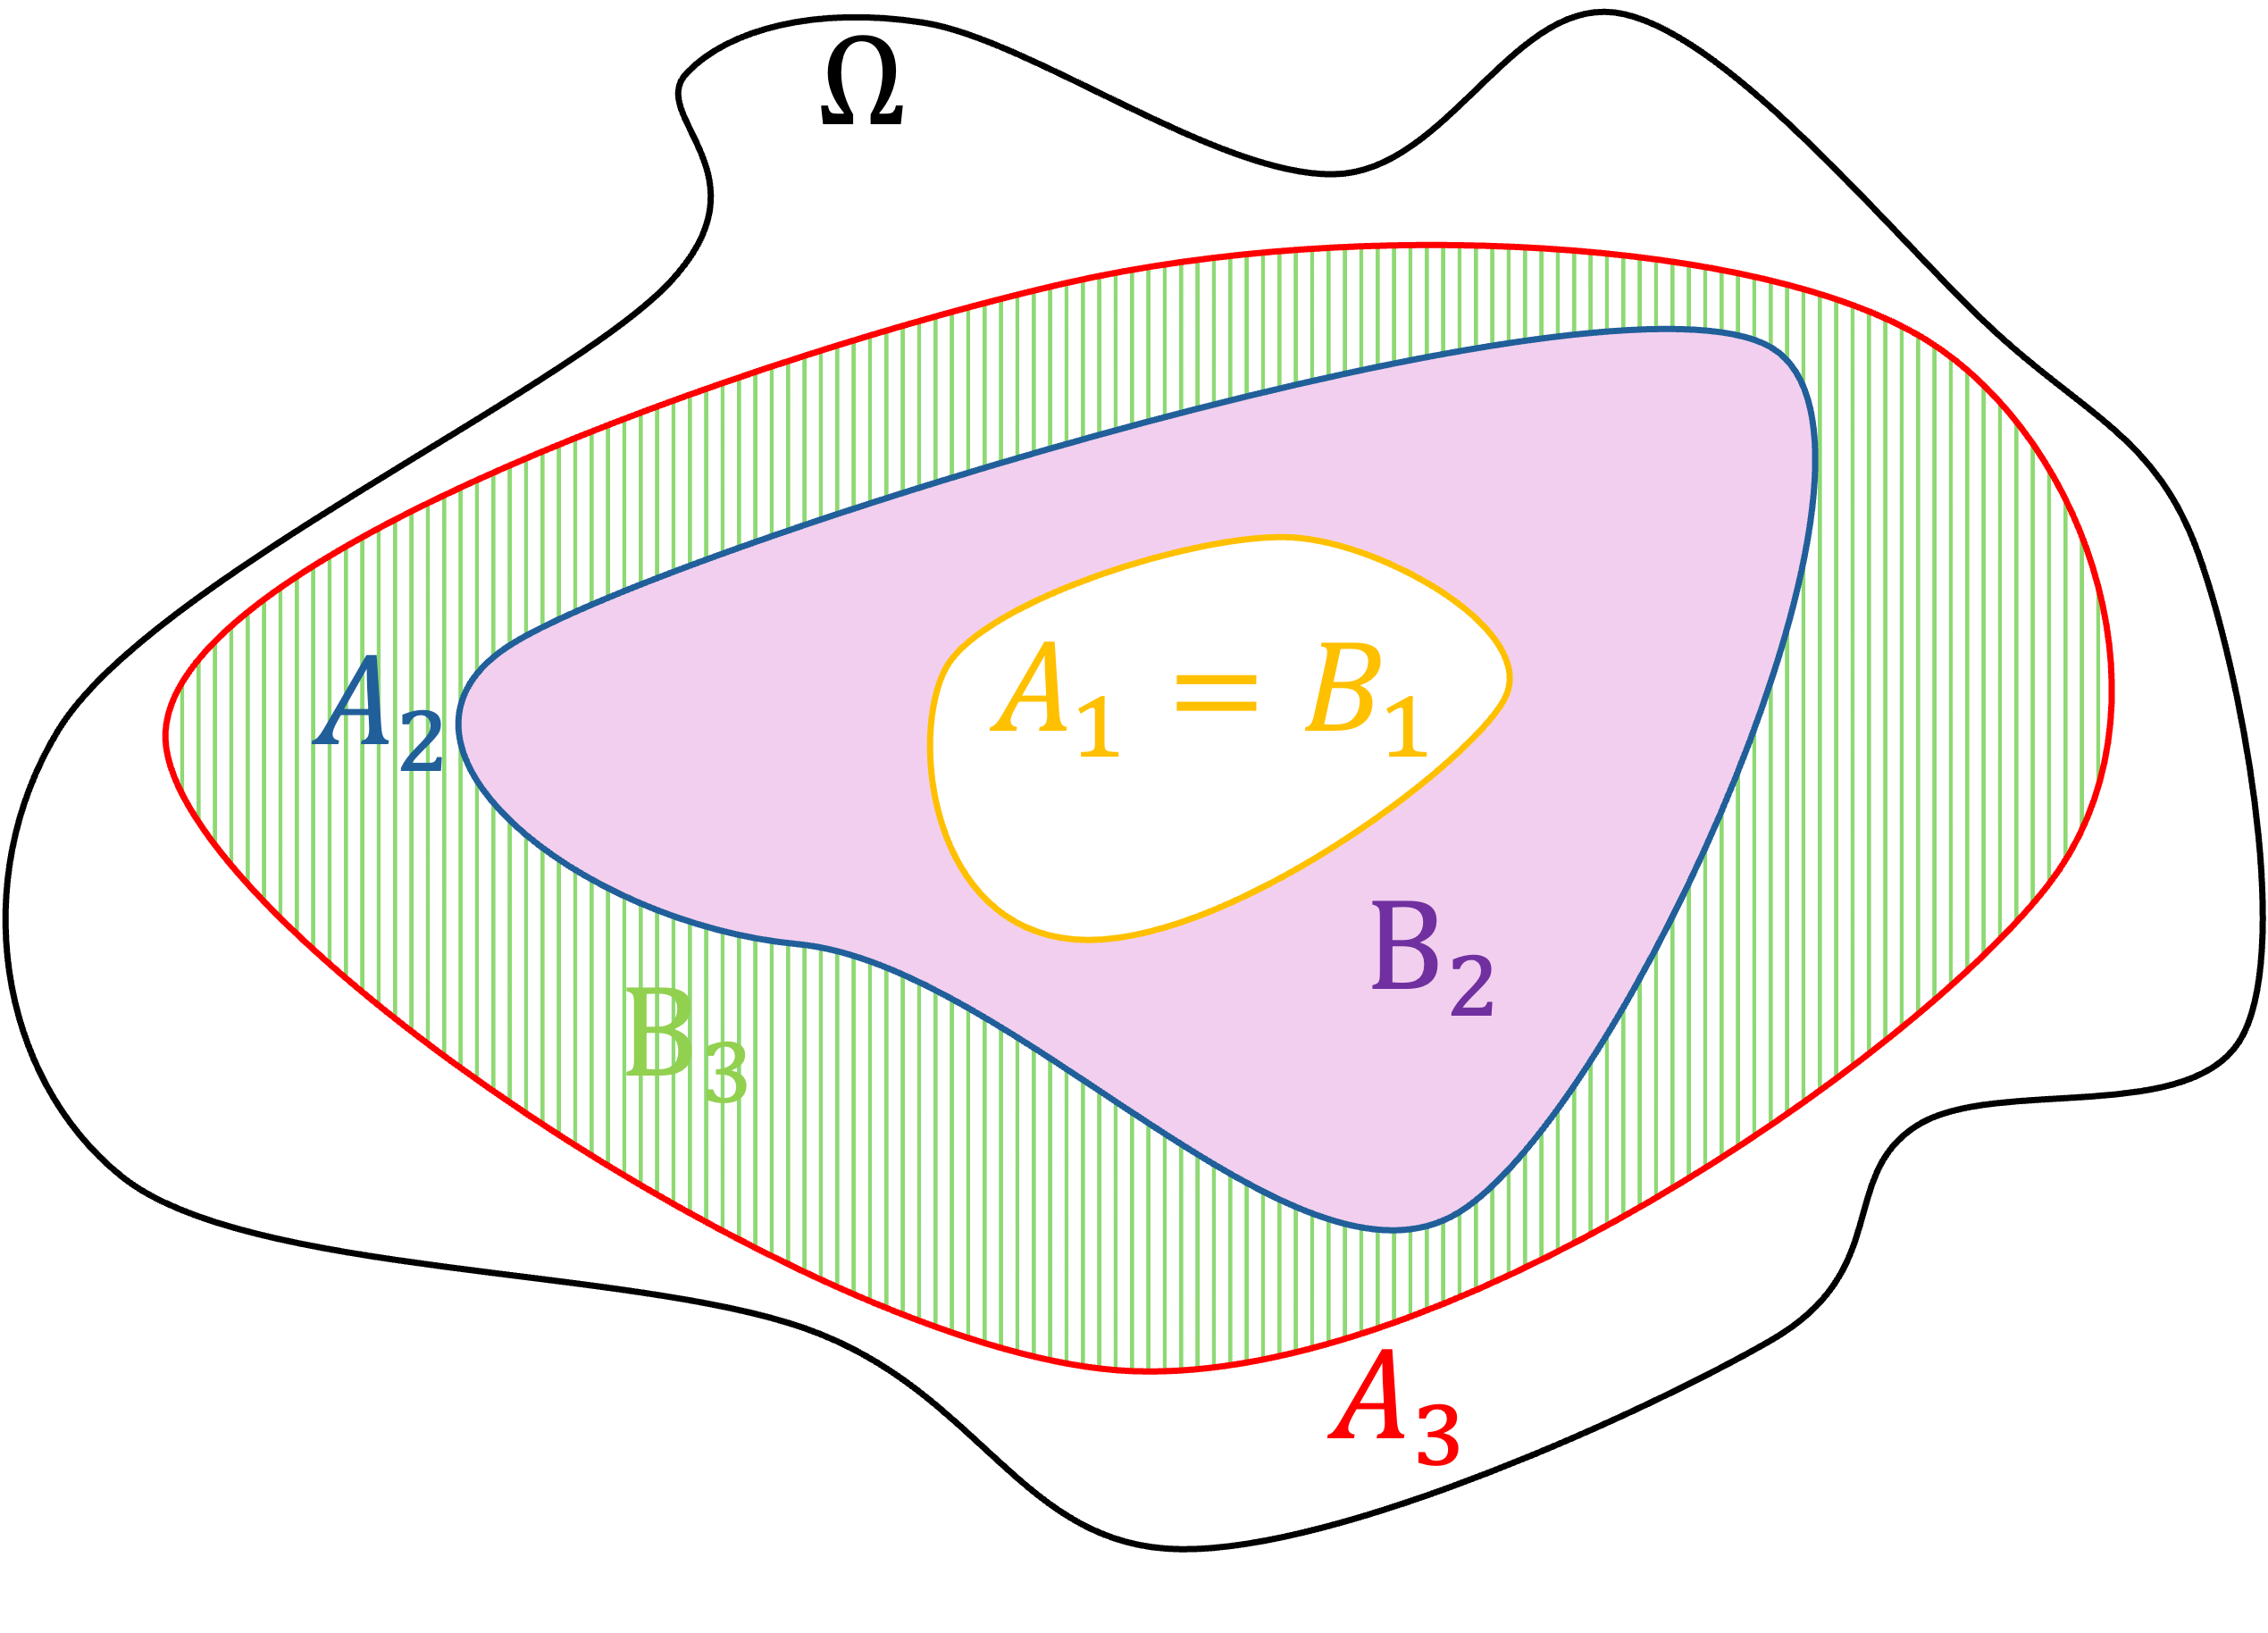
\includegraphics[width=0.7\linewidth]{Media/Dim_2.6..png}
    \end{minipage}
    \]
    Dove si ha che 
    \begin{itemize}
        \item I $B_k$ sono disgiunti a 2 a 2;
        \item $A_n = \bigcup_{k=1}^\infty B_k$ (quindi vale la finita additività);
        \item $\overline{A} = \bigcup_n A_n = \bigcup_k B_k$.
    \end{itemize}
    \begin{align*}
        \Rightarrow \mathbb{P}(\overline{A}) = \mathbb{P}(\bigcup_{n=1}^\infty A_N) &\overset{(2)}{=} \mathbb{P}(\bigcup_k B_k) \overset{(\sigma-additività)}{=} \sum_{k=1}^\infty \mathbb{P}(B_k)\\
        &= \lim_{n\rightarrow+\infty} \sum_{k=1}^n \mathbb{P}(B_k) \overset{(2)}{=} \lim_{n\rightarrow+\infty}\sum_{k=1}^n \mathbb{P}(A_n) 
    \end{align*}
    \end{dimostrazione}
\end{teorema}

\section{Assegnare una Probabilità con $\Omega$ Discreto}\label{sec:omega-discreto}
Definito uno spazio di Probabilità $(\Omega, \mathcal{A}, \mathbb{P})$, se avessimo un $\Omega$ qualsiasi, $\mathcal{A}$ potrebbe essere molto grande. Difatti già se prendessimo $\Omega = \{1, \dots, N\}$ e $\mathcal{A}=\mathcal{P}(\Omega )$ avremmo che la cardinalità di $\mathcal{A}$ risulterebbe essere $|\mathcal{A}| = 2^N$.\\
\\
Imponiamo quindi (per il momento) che $\Omega$ sia discreto, ovvero finito o al più numerabile. D'ora in avanti, qualora $\Omega$ fosse discreto, prenderemo $\mathcal{A} = \mathcal{P}(\Omega)$, salvo diversa indicazione.

\begin{teorema}
\label{th:2.7}
     Sia $\Omega = \{\omega_n: \;\;\;n\in I\}$ con $I\subseteq \mathbb{N}$, allora vale che:
    \begin{enumerate}
        \item Ogni probabilità $\mathbb{P}$ su $(\Omega, \mathcal{P}(\Omega), \mathbb{P})$ è caratterizzata dai suoi valori sugli atomi $\{\omega_n\}$ con $n\geq 1$, ovvero che:
        \[p_n=\mathbb{P}(\{\omega_n\})\;\;\;n\geq1\]
        \item Sia $(p_n)_{n\geq 1}$ una successione di numeri reali: $\exists! \;\;\mathbb{P}:\mathcal{P}(\Omega)\rightarrow[0,1]$ misura di probabilità tale che:
        \[\mathbb{P}(\{\omega_n\})=p_n\;\;\;\forall n\geq 1\;\;\;\; \iff \;\;\;\; 
        \begin{cases}
         p_n \geq 0 \\
         \sum_{n\in I}p_n=1
        \end{cases}
        \]
    \end{enumerate}
\begin{dimostrazione}
    1) $A\in\mathcal{P}(\Omega): \quad A = \bigcup_{n\in J}\{w_n\} \quad \text{con } J\subseteq I$\\
    Allora avremo che: $\quad \mathbb{P}(A) \overset{\sigma-add}{=} \sum_{n\in J}\mathbb{P}(\{w_n\}) = \sum_{n\in J} p_n$.\\
    \\
    2) $(\Rightarrow) \quad$ Siccome $p_n = \mathbb{P}(w_n)\in[0, 1]\quad \Rightarrow p_n \geq 0$ risulta essere sempre vera. Inoltre siccome $\Omega = \bigcup_{n\in I}\{w_n\}$ si ha che:
    \[\mathbb{P}(\Omega) \overset{\sigma-add}{=} \sum_{n\in I} \mathbb{P}(\{w_n\}) = \sum_{n\in I}p_n \overset{\mathbb{P}(\Omega)=1}{=}1\]
    $(\Leftarrow) \quad \begin{cases}
         p_n \geq 0 \\
         \sum_{n\in I}p_n=1
        \end{cases}
        \qquad \text{con} \qquad A = \bigcup_{n\in J}\{w_n\}$. \\
        Definisco $\mathbb{P}(A) = \bigcup_{n\in J}p_n$. Si dimostra che $\mathbb{P}$ è una misura di probabilità, ovvero che $\mathbb{P}(\Omega) = 1$ e vale la $\sigma$-additività (che non dimostreremo):
        \[\Omega = \bigcup_{n\in I}\{w_n\}\quad\Rightarrow\quad \mathbb{P}(\Omega) = \sum_{n\in I}p_n = 1\]
\end{dimostrazione}
\end{teorema}

\subsection{Esempi Notevoli di Modelli Discreti}
Esistono molti modelli discreti, ma ne riportiamo i più comuni.\\
\\
\(\bigstar\) Si prenda l'esempio nel quale si pescano delle palline numerate, dove: si hanno $N$ palline numerate (indistinguibili per il resto), $\Omega = \{1, \dots, N\}$ e $\mathcal{A} = \mathcal{P}(\Omega)$. \\
\\
Come trovo $\mathbb{P}$?\\
Una soluzione sarebbe quella di cercare $p_1, \dots, p_N$, consapevoli del fatto che \(p_n = \mathbb{P}(\{n\})\).

\[
\begin{cases}
    p_1 = p_2 = \dots = p_n = c\\
    \begin{array}{l}
        p_n \ge 0\\[3pt]
        \sum_{n=1}^N p_n = 1
    \end{array}
\end{cases}
\Rightarrow \quad 
\begin{cases}
    c\geq0\\
    \sum_{n=1}^N c = Nc = 1
\end{cases}
\quad \Rightarrow \quad c = \frac{1}{N}
\]\\
Dove la prima condizione deriva direttamente da come è stato costruito l'esperimento, mentre le altre due sono necessarie affinché sia una probabilità. Questo che abbiamo appena costruito è il \textbf{Modello Uniforme} $(\Omega, \mathcal{P}(\Omega), \mathbb{P}_{uni})$, che formalizzato risulta essere:
\[A\in\mathcal{P}(\Omega),\quad \mathbb{P}(A) = \frac{|A|}{|\Omega|} = \frac{\text{Casi favorevoli}}{\text{Casi possibili}}\]
Dove: 
\[|\Omega| \le +\infty \iff (p_n)_{n\geq1}: \boxed{p_n = \frac{1}{N} = \frac{1}{|\Omega|}}\]\\
\\
\(\bigstar\) Costruiamo adesso il \textbf{Modello Binomiale}. Siano:
\[\Omega = \{0, ..., n\}, n\in \mathbb{N};\quad p\in[0, 1];\quad \mathcal{A} = \mathcal{P}(\Omega)\]
Dunque $|\Omega| = n+1\;$ e $\;|\mathcal{A}| = 2^{n+1} $. Si avrà il modello binomiale $(\Omega, \mathcal{P}(\Omega), \mathbb{P}_{bin})$ se e solo se:
\[\boxed{p_k = \binom{n}{k} p^k(1-p)^{n-k}}\quad k:0, \dots, n\]
Si può mostrare (non tanto facilmente) che: 
\(\begin{cases}
    \sum_{k=0}^np_k = 1\\
    p_k \geq 0
\end{cases}\) concludendo che $\mathbb{P}_{bin}$ è una probabilità.\\
\\
\(\bigstar\) L'ultimo esempio è il \textbf{Modello di Poisson}, dove:
\[\Omega = \mathbb{N}, \quad \mathcal{A} = \mathcal{P}(\Omega); \quad \boxed{p_n = e^{-\lambda}\frac{\lambda^n}{n!}}\]

\chapter{Assegnare una Probabilità con $\Omega$ Qualsiasi}
In questo capitolo cercheremo di affrontare la casistica in cui il nostro spazio campionario non sia per forza discreto, come fatto in precedenza. Per aiutarci in ciò, distingueremo due casistiche: un caso \textit{"semplice"} ed un caso più complesso con $\Omega \subseteq \mathbb{R}$.
\section{Caso ``Semplice": Classi di Eventi}\label{sec:caso-semplice}
In questa trattazione avremo sì $\Omega$ generico, ma ci interesserà solo una classe ristretta di eventi $\mathcal{C}$, che quindi contiene sottoinsiemi di $\Omega$.
\begin{definizione}
    Data $\mathcal{C}\in \mathcal{P}(\Omega)$ una classe (o famiglia) di sottoinsiemi si definisce $\sigma(\mathcal{C})$ la più piccola $\sigma$-algebra che contiene $\mathcal{C}$, e la si denota con "$\sigma$-algebra generata dalla classe $\mathcal{C}$"
\end{definizione}
\begin{proposizione}
    Per qualsiasi classe $\mathcal{C}$ di sottoinsiemi di $\Omega$, esiste sempre $\sigma(\mathcal{C})$
\end{proposizione}

Si osservi che anche se $\mathcal{C} \subseteq \mathcal{P}(\Omega)$ (dove l'insieme delle parti è una $\sigma$-algebra), questo non implica che $\mathcal{C}$ contenga una $\sigma$-algebra di $\Omega$.\\
\\
Per costruire $\sigma(\mathcal{C})$ si parte dall'insieme $\mathcal{F}$ definito come: $\mathcal{F} = \{\mathcal{A}_\alpha: \mathcal{A}_\alpha\supseteq\mathcal{C}\}$, ovvero l'insieme che contiene tutte le $\sigma$-algebre che contengono $\mathcal{C}$. A questo punto, la $\sigma$-algebra generata da $\mathcal{C}$ risulta essere
\[\sigma(\mathcal{C}) = \bigcap_\alpha \mathcal{A}_\alpha\]
Dove l'intersezione rimane una $\sigma$-algebra ed è per costruzione la più piccola.
\begin{definizione}
    Si dice che $\;\mathcal{C} = \{C_k: k\in I\}\subseteq \mathcal{P}(\Omega)$ è una partizione discreta di $\Omega$ se:
    \begin{enumerate}
        \item $I\subseteq\mathbb{N}$ \hfill \textit{(ossia che $I$ è finito o al più numerabile)}
        \item $C_k \cap C_h = \varnothing \quad \forall h\neq k$
        \item $\bigcup_{k\in I} C_k = \Omega$
    \end{enumerate}
\end{definizione}

Si presti attenzione che $\mathcal{C}$ è  una famiglia di insiemi $C_k$ (visti come insiemi unici), tuttavia se faccio l'unione di (per esempio) $C_1\cup C_2$, questo potrebbe non stare in $\mathcal{C}$.\\
\\
Da un punto di vista modellistico, partizionare $\Omega$ ci permette di far "realizzare" almeno un (ed uno solo, in quanto sono disgiunti) evento della classe $\mathcal{C}$.
\begin{figure}[H]
    \centering
    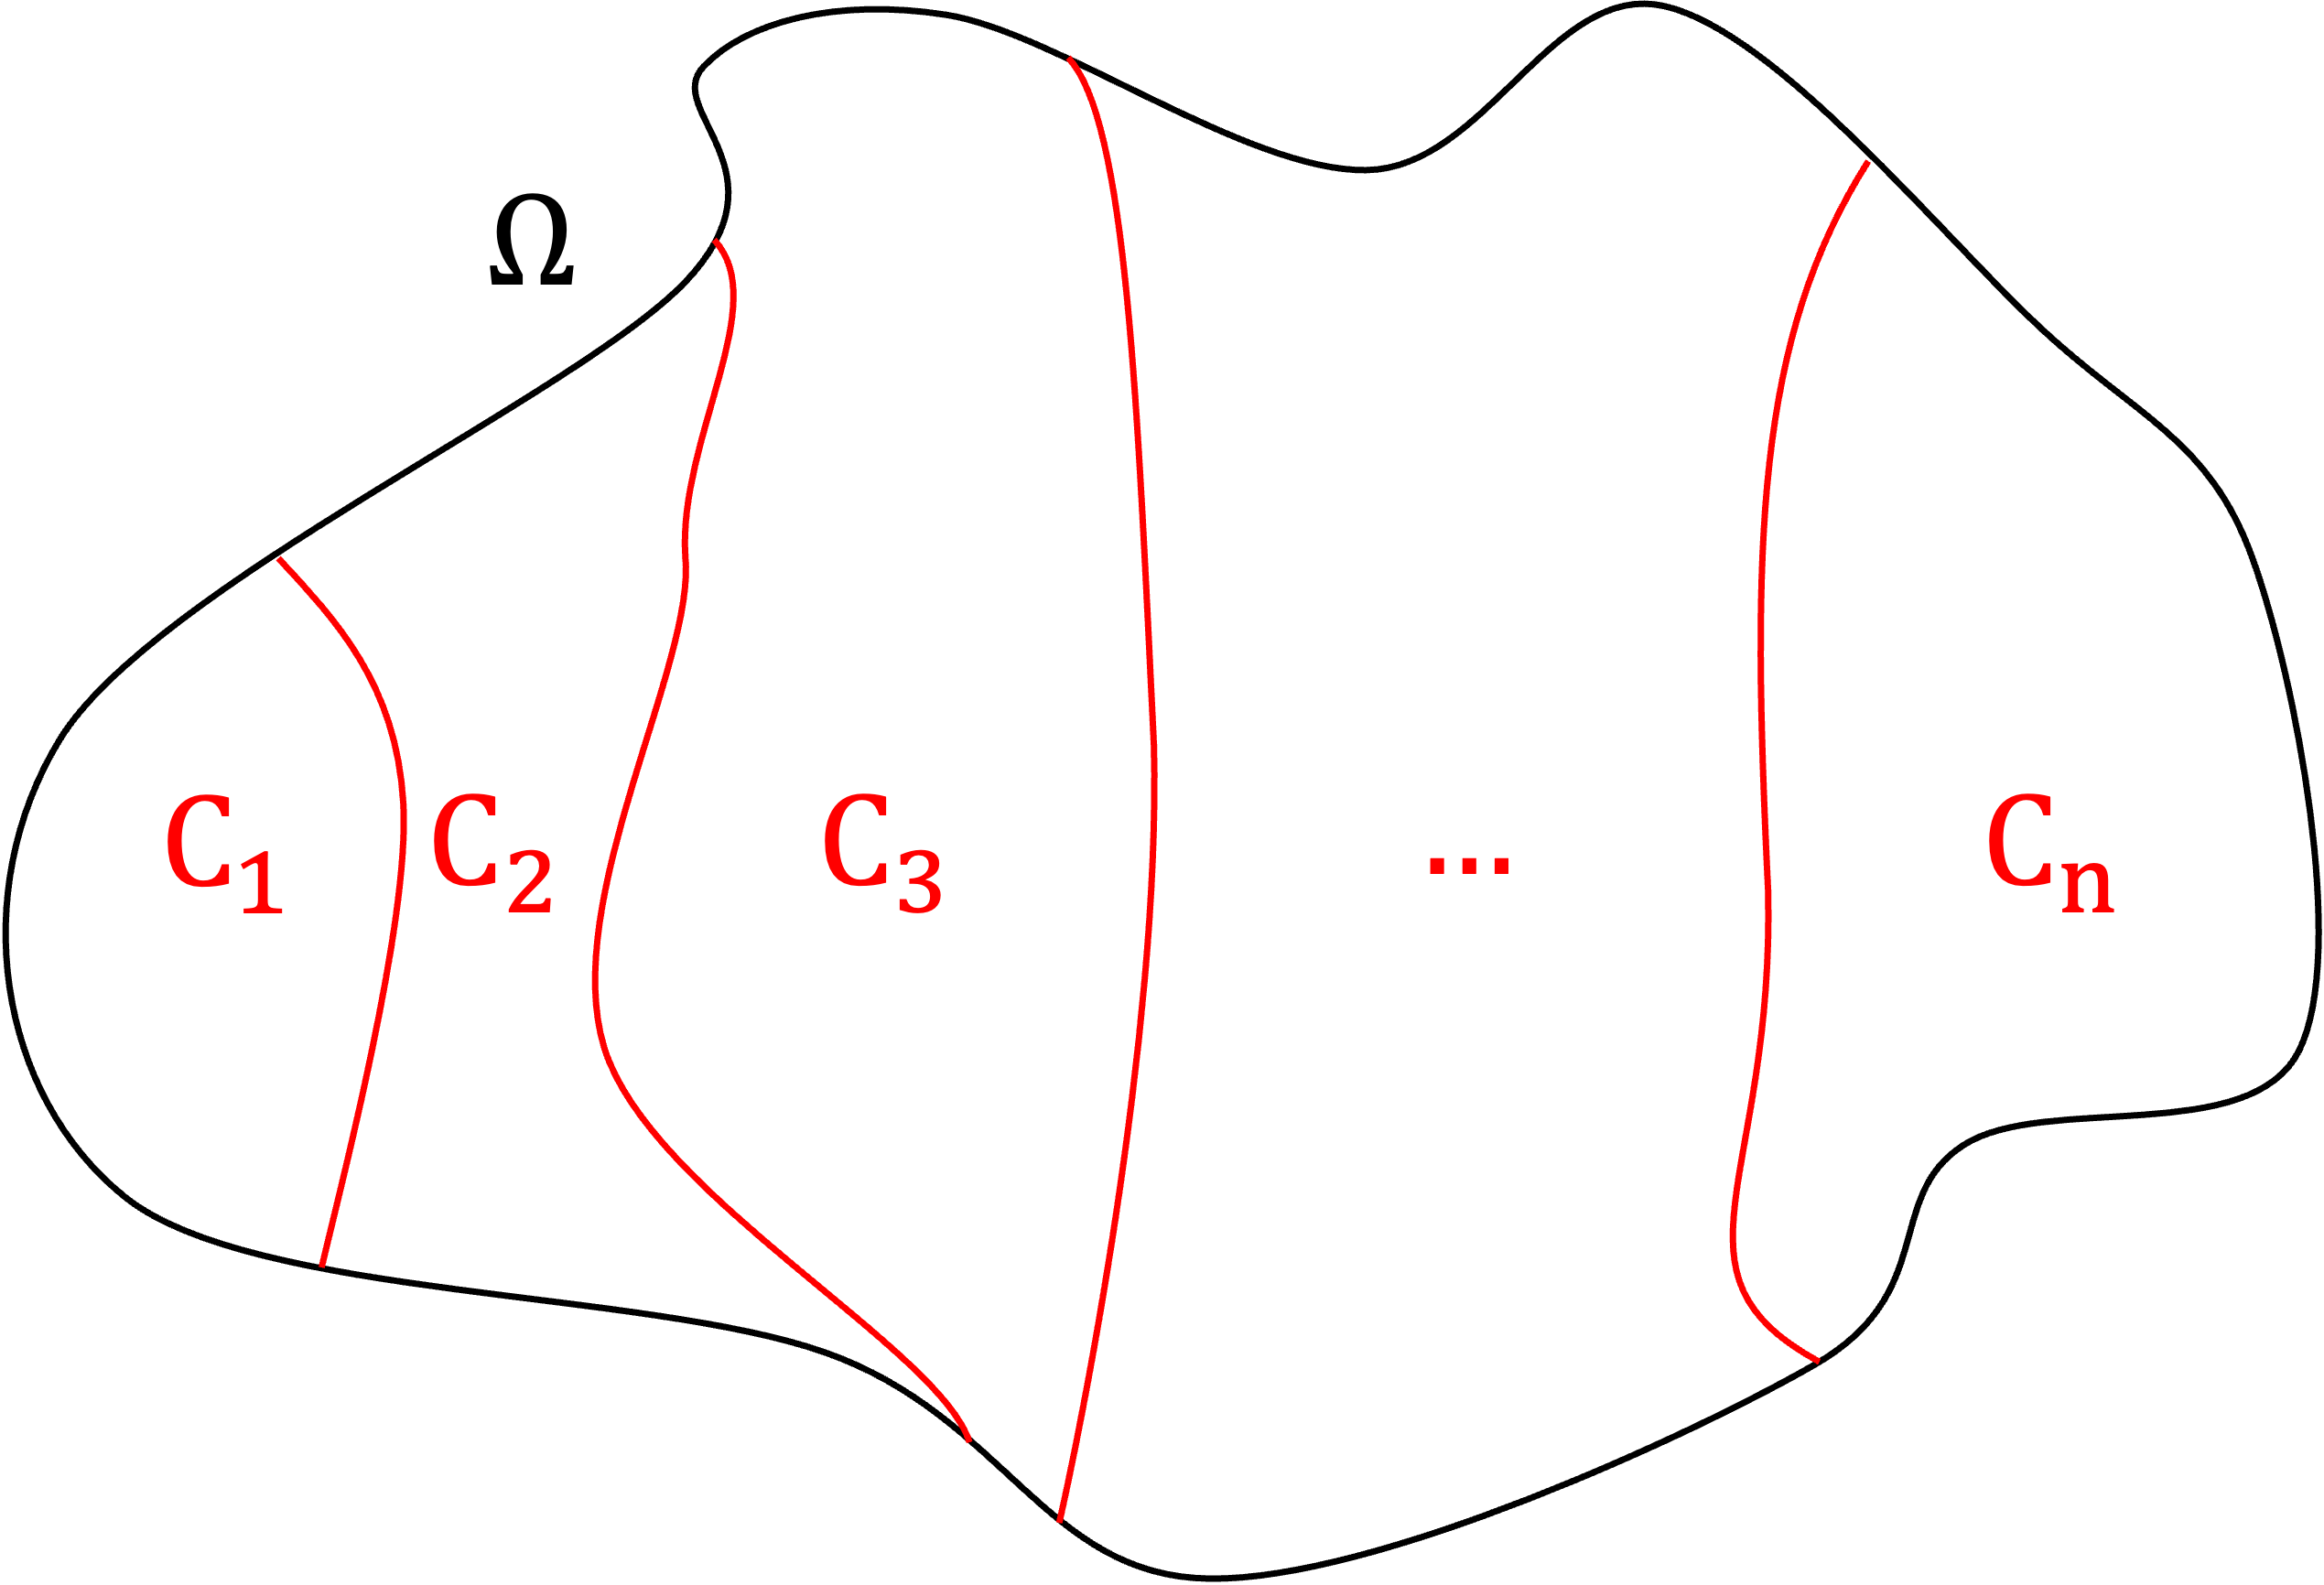
\includegraphics[width=0.3\linewidth]{Media/Partizione.png}
    \caption{Esempio grafico di una partizione}
    \label{fig:placeholder}
\end{figure}

\begin{esempio}
    Consideriamo $\mathbb{R}^+ = \bigcup_{n=1}^\infty[n-1, n)\;$ con $\;C_n = [n-1, n)$. \\Allora $\;\mathcal{C} =\{ C_n: n\in[1, + \infty)\}$ è una partizione di $\mathbb{R}^+$ diversa da $\mathcal{P}(\Omega)$. Siamo quindi riusciti ad isolare una classe al più numerabile.
\end{esempio}

\begin{proposizione}
    Quando $\mathcal{C}$ è una partizione discreta di $\Omega$, allora:
    \[\mathcal{A} = \sigma (\mathcal{C}) = \set{A \subseteq \Omega \quad| \quad A  = \bigcup_{j\in J}C_j, \quad J\subseteq I}\]
\end{proposizione}

Questa proposizione ci permette di vedere gli elementi della partizione come "atomi": in un certo senso sono l'unità più piccola. Non posso far altro che unire due elementi $C_h$ e $C_k$, non posso scindere in parti più piccole.

\begin{esempio}
    Nell'esempio precedente, posso solo dire quale intervallo si è \textit{acceso}, ma non ho un livello di dettaglio maggiore.
\end{esempio}
Abbiamo quindi capito che dato un $\Omega$ qualsiasi con $\mathcal{C}$ sua partizione discreta, allora ci conviene prendere $\mathcal{A} = \sigma (\mathcal{C})$. Ma come assegno $\mathbb{P}$?
\begin{teorema}
    Dato $\Omega$ qualsiasi e $\mathcal{C}$ una sua partizione discreta, allora:
    \begin{enumerate}
        \item Ogni $\mathbb{P}$ su $(\Omega, \sigma(\mathcal{C}))$ è univocamente determinata da 
        \[p_n = \mathbb{P}(C_n)\]
        Infatti $\forall A \in \sigma(\mathcal{C}), \quad A \overset{(3.4)}{=} \bigcup_{j\in J}C_j,\quad J\subseteq I:$
        \[\mathbb{P}(A) = \mathbb{P}\left(\bigcup_{j\in J}C_j\right) \overset{\sigma-add}{=} \sum_{j\in J}\mathbb{P}(C_j)  = \sum_{j \in J} p_j\]
        \item Data una successione $(p_n)_{n\geq1}$ di numeri reali, allora:
        \[
        \exists!\;\mathbb{P}:\sigma(\mathcal{C})\rightarrow[0, 1] \quad t.c. \quad \mathbb{P}(C_n) = p_n 
        \quad \iff \quad
        \begin{cases}
            p_n \geq 0 \quad \forall n\in I \\
            \sum_{n \in I} p_n = 1
        \end{cases}
        \]
    \end{enumerate}
\end{teorema}

\section{Probabilità Condizionata}

La probabilità (che di per se è una misura di quanto un evento è lecito pensare che accada), è influenzata dalla quantità di informazioni che abbiamo a disposizione. La probabilità condizionata misura quanto un evento A diventa probabile una volta che sappiamo che un altro evento B è accaduto.\\
\\
Non è più una probabilità “assoluta”, ma una probabilità relativa ad un contesto (o ad un'informazione aggiuntiva che abbiamo). \\
\\
Poniamoci nell'esperimento dove si lanciano 2 dadi, se volessimo calcolare la probabilità dell'evento $A =$ \textit{"la somma dei dadi è 12"}, allora potremmo calcolarla banalmente come $\mathbb{P}(A) = \frac{|A|}{|\Omega|} = 1/36$.\\
Se però consideriamo l'evento $E = $\textit{"Sul primo dado esce 6"}, e volessi capire $\mathbb{P}(A)$ dato che l'evento $E$ si è verificato, è come se $E$ "diventasse" il nostro "nuovo" $\Omega$.
\begin{figure}[H]
    \centering
    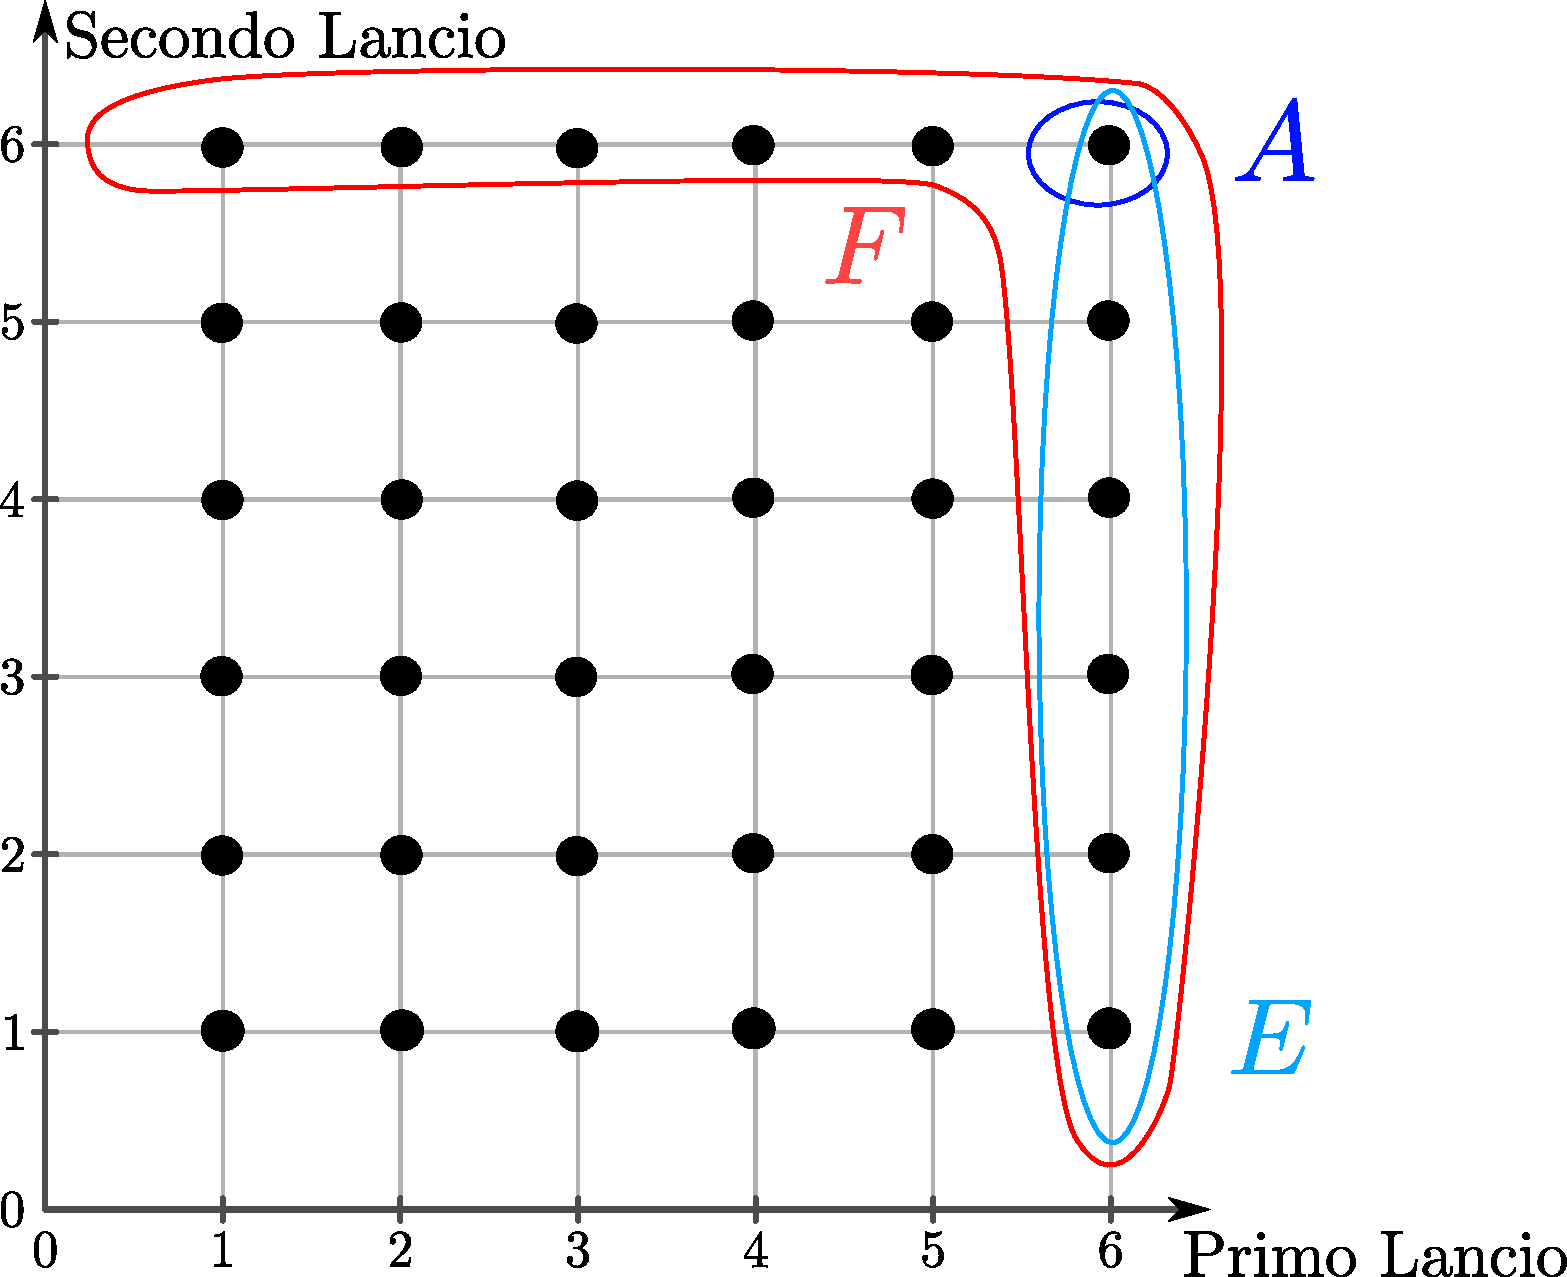
\includegraphics[width=0.4\linewidth]{Media/lanci.pdf}
\end{figure}
\noindent Come è facile intuire dal disegno avremo che la probabilità condizionata risulta essere:
\[\mathbb{P}(A \text{ "dato che si è verificato" }E) = \frac{|A\cap E|}{|E|} = \frac{|\{6, 6\}|}{6} = \frac{1}{6}\]
Se inoltre aggiungessimo l'evento $F = $ \textit{"Uno dei due dadi ha dato 6"}, ci aspetteremmo per buon senso che $\mathbb{P}(A \text{ "dato" }E) > \mathbb{P}(A\text{ "dato" }F)$, siccome sapere che si è verificato l'evento $E$ ci dà più informazioni rispetto all'evento $F$ (banalmente conosco su quale dei due dadi è uscito 6).\\
\\
Andiamo a formalizzare questi concetti in una solida teoria.

\begin{definizione}
    Dato $(\Omega, \mathcal{A}, \mathbb{P})$ spazio di probabilità e sia $E\subseteq \mathcal{A}$ un evento non trascurabile, i.e $\mathbb{P}(E) \gneq 0$. Allora $\forall A\in\mathcal{A}$ la probabilità condizionata di $A$ dato $E$ è il numero $\mathbb{P}(A|E)$:
    \[\mathbb{P}(A|E) = \frac{\mathbb{P}(A\cap E)}{\mathbb{P}(E)}\]
\end{definizione}
Dalla definizione vediamo immediatamente che è fondamentale che $\mathbb{P}(E)\neq 0$, altrimenti la scrittura non avrebbe senso matematico.\\
\\
Andando a riprendere l'esempio fatto precedentemente, ora che abbiamo un concetto formale di probabilità condizionata, e non più solo intuitivo, possiamo andare a calcolare le probabilità e confermare se i ragionamenti fatti in precedenza erano validi. \\
\[\mathbb{P} (A|E) = \frac{\mathbb{P}(A\cap E)}{\mathbb{P}(E)} = \frac{\mathbb{P}(\{6, 6\})}{\mathbb{P}\left(\{6, k\}; \;k\in\{1, ..., 6\}\right)} = \frac{\frac{|A\cap E|}{|\Omega|}}{\frac{|E|}{|\Omega|}} = \frac{|A\cap E|}{|E|} = \frac{1}{6}\]
Facendo lo stesso ragionamento con l'evento $F$:
\[\mathbb{P}(A|F) = \frac{\mathbb{P}(A \cap F)}{\mathbb{P}(F)} = \frac{|A\cap F|}{|F|} = \frac{1}{11} < \frac{1}{6}\]
dimostrando che l'intuizione che avevamo avuto sul fatto che $\mathbb{P}(A |E) > \mathbb{P}(A|F)$ era corretta.\\
\\
Osserviamo anche che dato un evento generico $E\in\mathcal{A}$ non trascurabile, allora possiamo definire $\mathbb{P}(A|E) = \frac{\mathbb{P}(A\cap E)}{\mathbb{P}(E)}$. Questo ci porta a dei casi limite:
\begin{itemize}
    \item Supponendo che $A\subseteq E:\quad \mathbb{P}(A|E) = \frac{\mathbb{P}(A\cap E)}{\mathbb{P}(E)} = \mathbb{P}(A|E) = \frac{\mathbb{P}(E)}{\mathbb{P}(E)} = 1$
    \item Se $A \text{ ed }E$ sono incompatibili\footnote{Ovvero che $E\cap A=\varnothing$}: $\quad\mathbb{P}(A|E) = 0$.
\end{itemize}

\begin{proposizione}
\label{prop:mappa_condizionata}
    Sia $E \in \mathcal{A}$ un evento non trascurabile. Allora la mappa:
    \[
    A \longmapsto \mathbb{P}(A \mid E) := \mathbb{P}_E(A)
    \]
    è una misura di probabilità su $\mathcal{A}\rightarrow [0,1]$.
\end{proposizione}
Questa proposizione ci permette di vedere la probabilità condizionata come una misura di probabilità, facendo così valere tutte le proprietà studiate sin ora.
\begin{esempio}
    Vale la proprietà $\quad \mathbb{P}(A^c|E) = 1 - \mathbb{P}(A|E)$, che scrivendola con la notazione più compatta diventa: $\quad \mathbb{P}_E(A^c) = 1 - \mathbb{P}_E(A) $
\end{esempio}
\bigskip
\noindent
\begin{tikzpicture}
  \draw[dashed] (0,0) -- (\textwidth,0);
\end{tikzpicture}\\
\\
Arrivati a questo punto vorremmo \textit{unire} i concetti di partizione e probabilità condizionata.\\
Vedremo infatti che si può partire da due partizioni di uno stesso spazio campionario $\Omega$, per ottenerne una terza, più \emph{fine}, che ne rappresenta tutte le possibili intersezioni. Inoltre, vorremo studiare come le probabilità associate a tali eventi intersezione possono essere calcolate a partire dalle probabilità condizionate.\\
\\
Possiamo rappresentare la struttura delle probabilità condizionate tramite un albero, in cui dal nodo radice $\Omega$ si diramano i rami verso gli eventi $A_n$, e da ciascun $A_n$ partono i sotto-rami verso gli eventi $B_k$.
\begin{center}
\begin{tikzpicture}[
  level distance=1.9cm,
  level 1/.style={sibling distance=35mm},
  level 2/.style={sibling distance=10mm},
  every node/.style={font=\small},
  edge from parent/.style={draw,-}
]
  % Nodo radice
  \node (root) {$\Omega$}
    % --- A1 ---
    child { node (A1) {$A_1$}
      child { node {$A_1 \cap B_1$}
              edge from parent node[pos=.60,above left] {\textcolor{red}{$q_{1|1}$}} }
      child { node {$\cdots$} }
      child { node {$A_1 \cap B_k$}
              edge from parent node[pos=.60,above right] {\textcolor{red}{$q_{k|1}$}} }
      edge from parent node[pos=.55,above left] {\textcolor{red}{$p_1$}}
    }
    % --- A2 ---
    child { node (A2) {$A_2$}
      child { node {$A_2 \cap B_1$}
              edge from parent node[pos=.60,above left] {\textcolor{red}{$q_{1|2}$}} }
      child { node {$\cdots$} }
      child { node {$A_2 \cap B_k$}
              edge from parent node[pos=.60,above right] {\textcolor{red}{$q_{k|2}$}} }
      edge from parent node[pos=.55,above] {\textcolor{red}{$p_2$}}
    }
    % --- puntini ---
    child { node {$\cdots$} }
    % --- An ---
    child { node (An) {$A_n$}
      child { node {$A_n \cap B_1$}
              edge from parent node[pos=.60,above left] {\textcolor{red}{$q_{1|n}$}} }
      child { node {$\cdots$} }
      child { node {$A_n \cap B_k$}
              edge from parent node[pos=.60,above right] {\textcolor{red}{$q_{k|n}$}} }
      edge from parent node[pos=.55,above right] {\textcolor{red}{$p_n$}}
    };
\end{tikzpicture}
\end{center}
Dove in rosso troviamo le probabilità degli eventi sottostanti, e per semplicità di notazione si è usato $\; q_{t|h} = \mathbb{P}(B_t|A_h)$.\\
\\
Ponendo la questione in maniera formale:
\\
Sia $(A_n : n \in I)$ una partizione discreta di $\Omega$ formata da eventi non trascurabili.
Analogamente, sia $(B_k:k \in I)$ un'altra partizione discreta dello stesso spazio campionario $\Omega$.
Ciascuna partizione suddivide $\Omega$ in eventi disgiunti e la loro unione ricopre tutto lo spazio.\\
\\
Dalle due partizioni possiamo ottenere una partizione \emph{più fine}, data dalle loro intersezioni:
\[
(A_n \cap B_k : n, k \in I),
\]
che costituisce ancora una partizione discreta di $\Omega$.
% --- DIAGRAMMA PARTIZIONE ---
\begin{center}
\begin{tikzpicture}[scale=0.5, every node/.style={font=\small}]
  % rettangolo esterno
  \draw[thick] (0,0) rectangle (9,5);
  \node[right] at (9,2.5) {$\Omega$};

  % linee verticali (partizione A)
  \foreach \x in {3,6}
    \draw[thick] (\x,0) -- (\x,5);

  % linee orizzontali (partizione B)
  \foreach \y in {1,2,3,4}
    \draw[orange, thick] (0,\y) -- (9,\y);

  % etichette A
  \node[below] at (1.5,0) {$A_1$};
  \node[below] at (4.5,0) {$A_2$};
  \node[below] at (5.8,0) {$\cdots$};
  \node[below] at (7.5,0) {$A_n$};

  % etichette B
  \node[left, orange] at (0,0.5) {$B_1$};
  \node[left, orange] at (0,1.5) {$B_2$};
  \node[left, orange] at (0,2.5) {$B_3$};
  \node[left, orange] at (0,4.0) {$\vdots$};
  \node[left, orange] at (0,4.7) {$B_k$};

  % rettangolo evidenziato per A2 ∩ B3
  \filldraw[fill=violet!20, draw=violet, thick] (3,2) rectangle (6,3);
  \node at (4.5,2.5) {\textcolor{violet}{$A_2 \cap B_3$}};
\end{tikzpicture}
\end{center}
Supponiamo di conoscere le probabilità
\(p_n = \mathbb{P}(A_n), \quad q_{k|n} = \mathbb{P}(B_k \mid A_n).\)\\
\\
La domanda naturale è: \textit{come posso determinare la probabilità dell’intersezione $\mathbb{P}(A_n \cap B_k)$? Ha senso (ed è corretto) calcolarla come:}
\[
\mathbb{P}(A_n \cap B_k) = \mathbb{P}(A_n) \cdot \mathbb{P}(B_k \mid A_n)?
\]
dato che $A_n$ sono tutti eventi non trascurabili, e di conseguenza vale la formula della probabilità condizionata?

\begin{teorema}
    Siano $(A_n : n \in I)$ e $(B_n : n \in I)$ partizioni discrete di eventi non trascurabili di $\Omega$. Siano:
    
    \begin{align*}
        &(p_n:n\geq1)\:\:\;:\;p_n\geq0\quad \:\:\:e \quad \sum_{n\in I}p_n = 1 \qquad \;\;\forall n\geq1 \\
        &(q_{k|n}:k\geq1)\;:\;q_{k|n}\geq0\quad e \quad \sum_{k\in I}q_{k|n} = 1 \qquad \forall k\geq1
    \end{align*}
    \[\Rightarrow\quad \exists!\; \mathbb{P} \text{ su } \mathcal{A} = \sigma\Big((A_n\cap B_k):\;n, k\in I\Big) \quad \text{t.c.} \quad
    \mathbb{P}(A_n) = p_n\quad  \text{e}\quad \mathbb{P}(B_k\mid A_n) = q_{k|n} \]
    \begin{dimostrazione}
        Solo per prova orale.
    \end{dimostrazione}
\end{teorema}

Grazie a questo teorema possiamo costruirci un modello conoscendo le probabilità condizionate!! \large\smiley
\begin{esempio}
    Si consideri un cesto contenente $n\geq2$ palline nere e $b\geq2$ palline bianche. Supponiamo di effettuare due estrazioni senza reimmissione. Consideriamo gli eventi:
    \begin{align*}
         N_1 &= \textit{"Alla prima estrazione pesco una nera"}\\
         N_1^c &= \textit{"Alla prima estrazione pesco una bianca"} = B_1\\
         N_2 &=\textit{"Alla seconda estrazione pesco una nera"}\\
         N_2^c & = \textit{"Alla seconda estrazione pesco una bianca"} = B_2
    \end{align*}
    Si avranno le seguenti probabilità condizionate:

\begin{center}
\begin{tikzpicture}[
  level distance=1.8cm,
  level 1/.style={sibling distance=60mm},
  level 2/.style={sibling distance=24mm},
  edge from parent/.style={draw,-,line width=0.9pt},
  every node/.style={font=\small}
]
  \node (root) {$\Omega$}
    % --- ramo N1 ---
    child { node (N1) {$N_1$}
      child { node {$N_1 \cap N_2$}
              edge from parent node[pos=.58,above left] {\textcolor{red}{$\dfrac{n-1}{\,n+b-1\,}$}} }
      child { node {$N_1 \cap B_2$}
              edge from parent node[pos=.58,above right] {\textcolor{red}{$\dfrac{b}{\,n+b-1\,}$}} }
      edge from parent node[pos=.55,above left] {\textcolor{red}{$\dfrac{n}{\,n+b\,}$}} }
    % --- ramo B1 ---
    child { node (B1) {$B_1$}
      child { node {$B_1 \cap N_2$}
              edge from parent node[pos=.58,above left] {\textcolor{red}{$\dfrac{n}{\,n+b-1\,}$}} }
      child { node {$B_1 \cap B_2$}
              edge from parent node[pos=.58,above right] {\textcolor{red}{$\dfrac{b-1}{\,n+b-1\,}$}} }
      edge from parent node[pos=.55,above right] {\textcolor{red}{$\dfrac{b}{\,n+b\,}$}} };
\end{tikzpicture}
\end{center}
Quindi si avrà che, per esempio: \[\mathbb{P}(N_1\cap B_2) = \frac{b}{n+b-1} \cdot \frac{n}{n+b}\]
Ma se invece volessimo conoscere $\mathbb{P}(N_2)?$ Oppure $\mathbb{P}(N_1|N_2)?$
\end{esempio}
Per rispondere alla domanda nell'esempio, intruduciamo le seguenti formule.
\begin{teorema}
    Sia $(\Omega, \mathcal{A}, \mathbb{P})$ uno spazio di probabilità, e consideriamo una partizione discreta $(E_n)_{n\in I}\subseteq \mathcal{A}$ di $\Omega$, dove $I\in \mathbb{N}$. Allora valgono le seguenti:
    \begin{enumerate}
        \item $\forall A\in\mathcal{A}:\quad \boxed{\mathbb{P}(A) = \sum_{n\in I}\mathbb{P}(A\cap E_n)}$ \hfill \textit{(Formula di disintegrazione)}
        \item Se inoltre $\mathbb{P}(E_n)>0\;\forall n\in I$, allora: \[\boxed{\mathbb{P}(A) = \sum_{n\in I}\mathbb{P}(A\mid E_n)\cdot \mathbb{P}(E_n)} \qquad \quad\textit{(Formula delle probabilità totali)}\] 
    \end{enumerate}

    \begin{dimostrazione}
        Siccome $E_n$ è  una partizione di $\Omega$, posso vedere $A$ come 
\begin{center}
\begin{minipage}{0.48\textwidth}
\begin{align*}
    A &= A \cap \Omega 
   = A \cap \left(\bigcup_{n\in I} E_n\right)\\
   &= \bigcup_{n\in I} (A \cap E_n)
\end{align*}
\end{minipage}%
\hfill
\begin{minipage}{0.40\textwidth}
\begin{tikzpicture}[scale=0.8, every node/.style={font=\small}]

  % --- Rettangolo esterno (Omega) ---
  \draw[thick] (0,0) rectangle (6,3);
  \node[right] at (6,1.5) {$\Omega$};

  % --- Linee verticali (partizione E_i) ---
  \foreach \x in {1.2,2.4,3.6,4.8}
    \draw[thick] (\x,0) -- (\x,3);

  % --- Etichette E1 ... En ---
  \node[below] at (0.6,0) {$E_1$};
  \node[below] at (3.0,0) {$\cdots$};
  \node[below] at (5.4,0) {$E_n$};

  % --- Evento A (ellisse rossa interamente dentro Omega) ---
  \draw[thick, red] (2.3,1.5) ellipse (1.6cm and 0.8cm);
  \node[red] at (3.8,2.2) {$A$};

  % --- Zona tratteggiata viola all’interno di A ---
  \begin{scope}
    \clip (2.3,1.5) ellipse (1.6cm and 0.8cm);
    \fill[pattern=north east lines, pattern color=violet!70] (0,0) rectangle (6,3);
  \end{scope}

\end{tikzpicture}
\end{minipage}
\end{center}

1. Per $\sigma$-additività si ha che (o anche finita additività):
\begin{equation}
   \mathbb{P}(A) = \mathbb{P}\left(\bigcup_{n\in I} (A \cap E_n)\right)=\sum_{n\in I}\mathbb{P}(A\cap E_n)
   \label{eq:partizione_prob}
\end{equation}
2. Osservo che se $\mathbb{P}(E_n)>0\quad \forall n\in I$, allora:
\[
\mathbb{P}(A\cap E_n) = \mathbb{P}(E_n)\cdot\mathbb{P}(A\mid E_n)\quad \forall n\in I
\]
Sostituendo banalmente questa equazione nella \eqref{eq:partizione_prob}, otteniamo la formula delle probabilità totali.
\end{dimostrazione}
\end{teorema}

Si può intuire che la formula delle probabilità totali, la si usa quando si ha incertezza "sulla prima estrazione", ed è come se pesassi con i pesi $\mathbb{P}(E_n)$.

\begin{esempio}
    Continuiamo l'esempio precedente.\\
    Ci siamo interrogati su come potessimo calcolare $\mathbb{P}(N_2)$ e $\mathbb{P}(N_1\mid N_2)$, ed ora abbiamo la soluzione: con le probabilità totali.\\
    Possiamo vedere la nostra partizione $(E_n:n\in I)\text{ con }I=\{1, 2\}$ tale che:
    \[
    \begin{cases}
        E_1=N_1\\
        E_2=N_1^c=B_1
    \end{cases}
    \]
    Allora i calcoli diventano facili:
    \begin{align*}
        \mathbb{P}(N_2) &= \mathbb{P}(N_2\mid N_1)\cdot\mathbb{P}(N_1) + \mathbb{P}(N_2\mid B_1)\cdot\mathbb{P}(B_1)\\
        &=\frac{n-1}{n+b-1}\cdot \frac{n}{n+b} + \frac{n}{n+b-1}\cdot\frac{b}{n+b}\\
        &=\frac{n\cdot(n+b-1)}{(n+b)(n+b-1)}\\
        &= \frac{n}{n+b}\\
        \\
        \mathbb{P}(N_1\mid N_2) &=\frac{\mathbb{P}(N_1\cap N_2)}{\mathbb{P}(N_2)} = \frac{\mathbb{P}(N_1\mid N_2)\cdot \mathbb{P}(N_1)}{\mathbb{P}(N_2)} = \frac{\frac{n-1}{b+n-1}\cdot \frac{n}{b+n}}{\frac{n}{n+b}}\\
        &=\frac{n-1}{b+n-1}
    \end{align*}
\end{esempio}
\bigskip
\noindent Senza saperlo, in quest'ultimo calcolo, ci siamo ricavati una formula fondamentale nel calcolo delle probabilità, ovvero la formula di Bayes.
\begin{teorema}
    Sia $(\Omega, \mathcal{A}, \mathbb{P})$ uno spazio di probabilità, e sia $(E_n)_{n\in I}$ una partizione discreta di $\Omega$ tale che tutti i $E_n$ siano non trascurabili.\\
    \\
    Allora, $\forall A\in \mathcal{A} \text{ dove } \mathbb{P}(A)>0:$
    \[\boxed{
    \mathbb{P}(E_h\mid A) = \frac{\mathbb{P}(A\mid E_h)\cdot \mathbb{P}(E_h)}{\mathbb{P}(A)} = \frac{\mathbb{P}(A\mid E_h)\cdot \mathbb{P}(E_h)}{\sum_{n\in I}\mathbb{P}(A\mid E_n)\cdot \mathbb{P}(E_n)}
    }
    \]
    \begin{dimostrazione}
        Definizione di $\mathbb{P}(E_h\mid A)\quad"+"\quad$ formula delle probabilità totali. Sostanzialmente già svolta nel teorema.
    \end{dimostrazione}
\end{teorema}

\begin{teorema}
    Sia $(\Omega, \mathcal{A}, \mathbb{P})$ uno spazio di probabilità, e siano \[A_1, \dots, A_n \in \mathcal{A}:\quad \mathbb{P}(A_1\cap A_2\cap\dots\cap A_{n-1})>0\]
    Allora si avrà che:
    \[\mathbb{P}(A_1\cap A_2\cap\dots\cap A_n) = \mathbb{P}(A_1)\cdot\mathbb{P}(A_2\mid A_1)\cdot \mathbb{P}(A_3\mid A_1\cap A_2)\cdots\mathbb{P}(A_n\mid A_1\cap\cdots\cap A_{n-1})\]
    Questa è detta \textit{Formula di Moltiplicazione}.
\end{teorema}
    \begin{dimostrazione}
        È evidente che: 
        \[A_1\cap\cdots\cap A_{n-1} \subseteq A_1\cap\cdots\cap A_{n-2}\subseteq \cdots \subseteq A_1\cap A_2\subseteq A_1\]
        Allora per monotonia della probabilità: $\mathbb{P}(A_1\cap\cdots\cap A_k)>0\quad \forall k\in[2, n-1]$.\\
        Di conseguenza avremo che, per la definizione di probabilità condizionata: 
        \begin{align*}
            &\mathbb{P}(A_1)\cdot\mathbb{P}(A_2\mid A_1)\cdot \mathbb{P}(A_3\mid A_1\cap A_2)\cdots\mathbb{P}(A_n\mid A_1\cap\cdots\cap A_{n-1}) = \\
            &= \cancel{\mathbb{P}(A_1)}\frac{\cancel{\mathbb{P}(A_1\cap A_2)}}{\cancel{\mathbb{P}(A_1)}}\cdot
            \frac{\cancel{\mathbb{P}(A_1\cap A_2\cap A_3)}}{\cancel{\mathbb{P}(A_1\cap A_2)}}\cdots
            \frac{\mathbb{P}(A_1\cap\cdots\cap A_n)}{\cancel{\mathbb{P}(A_1\cap\cdots\cap A_{n-1})}}
        \end{align*}
    \end{dimostrazione}

Dalla dimostrazione risulta evidente come mai nelle ipotesi del teorema  chiediamo che $\mathcal{A}:\quad \mathbb{P}(A_1\cap A_2\cap\dots\cap A_{n-1})>0$.\\

\subsection{Indipendenza Stocastica}
In questo sottocapito andremo a studiare una delle "qualità" più utili (e che ci semplifica la vita) che possono avere due eventi: l'indipendenza stocastica.
\begin{definizione}
    Dato $(\Omega, \mathcal{A}, \mathbb{P})$, due eventi $A, B\in\mathcal{A}$ si dicono stocasticamente indipendenti (o indipendenti) se:
    \[\mathbb{P}(A\cap B) = \mathbb{P}(A)\cdot\mathbb{P}(B)\]
    A livello di notazione si indica con $A \ind B$.
\end{definizione}
\bigskip 
\noindent Come si può intuire, il concetto di indipendenza e di probabilità condizionata sono fortemente collegati, difatti se ipotizziamo che $\mathbb{P}(A), \mathbb{P}(B)>0$, e che $A \ind B$, allora:

\[\mathbb{P}(A\mid B) = \frac{\mathbb{P}(A\cap B)}{\mathbb{P}(B)}= \frac{\mathbb{P}(A)\mathbb{P}(B)}{\mathbb{P}(B)} = \mathbb{P}(A)\]
In parole povere: se $A \ind B$, $B$ non andrà ad influenzare in alcun modo $A$ (e viceversa).

\begin{esempio}
    Ritornando all'esempio dell'estrazione senza reimmissione: $N_1 \text{ e }N_2$ non sono indipendenti, in quanto: 
    \[\mathbb{P}(N_2\mid N_1) = \frac{n-1}{n+b-1}\neq \mathbb{P}(N_2) = \frac{n}{n+b}\]
    Se invece fossimo nel caso in cui estraiamo con reimmissione, allora avremmo che $N_1\ind N_2$ in quanto:
    \[\mathbb{P}(N_1\cap N_2)= \mathbb{P}(N_2\mid N_1)\cdot \mathbb{P}(N_1) = \frac{n}{n+b} = \mathbb{P}(N_1)\cdot\mathbb{P}(N_2)\]
\end{esempio}
\bigskip
\bigskip
\noindent A questo punto possiamo fare alcune osservazioni importanti.\\
\\
\(\bigstar\) Possiamo avere la presenza di due casi limite, con $\mathbb{P}(A)$ degenere e $\forall B$ (ovviamente potremmo scambiare A con B):
\begin{enumerate}
    \item Se $\mathbb{P}(A) = 0\quad\Rightarrow\quad \mathbb{P}(A\cap B)\leq\mathbb{P}(A) = 0 \quad\Rightarrow\quad \mathbb{P}(A\cap B) = \mathbb{P}(A)\mathbb{P}(B)$\\
    A livello modellistico questo ci dice che, qualunque sia $B$, questo è indipendente da un evento che ha probabilità $0$ di verificarsi.
    \item Se $\mathbb{P}(A) = 1$, allora possiamo scrivere $B = (A\cap B)\cup (A^c\cap B)$ e di conseguenza:
    \[\mathbb{P}(B) = \mathbb{P}(A\cap B) + \underbrace{\mathbb{P}(A^c \cap B)}_{=\,0\text{, dato che }\mathbb{P}(A^c) = 0}
    \]
    \[\Rightarrow\quad \mathbb{P}(A)\cdot\mathbb{P}(B) = \mathbb{P}(B) = \mathbb{P}(A\cap B)\]
    Anche in questo caso, se la probabilità di un evento $A$ è 1, qualsiasi altro evento consideriamo sarà indipendente $A$.
\end{enumerate}
\(\bigstar\) Se ipotizziamo che $A\cap B =\varnothing$, e che $\mathbb{P}(A), \mathbb{P}(B) > 0$, allora $A$ e $B$ \textbf{non} saranno mai indipendenti. Questo perchè:
\[\mathbb{P}(A\cap B) = 0 \neq \mathbb{P}(A)\mathbb{P}(B) > 0\]
Questo fatto ci pone davanti ad una realtà che può sembrare ingannevole: il fatto che due eventi siano indipendenti non ha niente a che fare col fatto che quest'ultimi siano disgiunti. La disgiunzione è una \textbf{forte} nozione di correlazione (se accade uno, non può accadere l'altro).\\
\\
\(\bigstar\) Se $A\ind B \quad\Rightarrow\quad A\ind B^c, A^c\ind B, A^c\ind B^c$\\
Possiamo esprimere questo concetto passando dalle $\sigma$-algebre generate dai due eventi:
\[A\ind B \quad \iff\quad\sigma(A)\ind \sigma (B)\]
Ossia che:
\begin{definizione}
\label{def:3.13}
$\mathcal{F,G}$ due $\sigma$-algebre su $\Omega$ sono indipendenti se:
\[\forall F\in \mathcal{F} \text{ e }\forall G\in\mathcal{G}: \quad G\ind F\]
\end{definizione}
\noindent Per convincerci di questo fatto, dimostriamo per esempio che se $A\ind B\Rightarrow A\ind B^c$:\\
Scrivendo $A = (A\cap B)\cup (A\cap B)$, allora $\mathbb{P}(A) = \mathbb{P}(A\cap B) + \mathbb{P}(A\cap B^c)$. Di conseguenza avremo che:
\begin{align*}
    \mathbb{P}(A\cap B^c)&=\mathbb{P}(A)- \mathbb{P}(A\cap B) = \mathbb{P}(A)- \mathbb{P}(A)\cdot \mathbb{P}(B) \\
    & = \mathbb{P} (A) [1 - \mathbb{P}(B)]\\
    & = \mathbb{P}(A)\mathbb{P}(B^c)
\end{align*}
Questa "dimostrazione" si può effettuare similmente per tutte le altre casistiche.

\begin{definizione}
    Sia $I$ un insieme di indici, $(A_i)_{i\in I}\subseteq\mathcal{A}$ è una famiglia di eventi (mutualmente) indipendenti se:
    \[\forall J\subseteq I\quad\text{t.c.}\quad 2\leq |J| < +\infty, \text{ vale che:}\qquad \mathbb{P}\left(\bigcap_{j\in J}A_j\right) = \prod_{j\in J}\mathbb{P}(A_j)\]
    
    \faWarning $\quad I$ può essere qualsiasi, la condizione deve essere verificata $\forall J\subseteq I$ finito.
\end{definizione}

\begin{esempio}
    Sia $\{A_1, A_2, A_3\}\subseteq\mathcal{A}$. Di conseguenza $I = \{1, 2, 3\}$. Dobbiamo verificare la condizione $\forall J:\quad 2\leq |J| < +\infty$. \\
    Ossia per:
    \begin{itemize}
        \item $\{1, 2\}\longrightarrow \mathbb{P}(A_1\cap A_2)=\mathbb{P}(A_1)\cdot \mathbb{P}(A_2)$
        \item $\{1, 3\}\longrightarrow \mathbb{P}(A_1\cap A_3)=\mathbb{P}(A_1)\cdot \mathbb{P}(A_3)$
        \item $\{2, 3\}\longrightarrow \mathbb{P}(A_2\cap A_3)=\mathbb{P}(A_2)\cdot \mathbb{P}(A_3)$
        \item $\{1, 2, 3\}\longrightarrow \mathbb{P}(A_1\cap A_2\cap A_3)=\mathbb{P}(A_1)\cdot \mathbb{P}(A_2)\cdot \mathbb{P}(A_3)$
    \end{itemize}
\end{esempio}
Vediamo quindi benissimo dall'esempio che la condizione di indipendenza di una famiglia di eventi, risulta essere molto complicata da verificare, in quanto le condizioni che devono essere verificate crescono esponenzialmente con la cardinalità $n$ di $I$; in particolare $\#_{\text{condizioni da verificare}} = 2^n - n - 1$.\\
\\
Si osservi inoltre che se $A_1, ..., A_n$ è una famiglia di eventi indipendenti, allora:
\[\forall k:1, ..., n\qquad \sigma(A_k)\ind \sigma(A_{\hat{k}})\qquad \text{dove } A_k=\{A_1, ..., A_{k-1}, A_{k+1}, ...A_n\}\]

\subsection{Indipendenza Condizionata}
Per concludere il capitolo, possiamo "mettere assieme" i concetti di indipendenza stocastica e probabilità condizionata. Questo non ci deve sorprendere, perché come abbiamo visto con la proposizione \eqref{prop:mappa_condizionata}, possiamo trattare la probabilità condizionata $\mathbb{P}_E$ come una probabilità.

\begin{definizione}
    Siano $A, B, E \in \mathcal{A};\;\mathbb{P}(E)>0$. Si dice che $A$ e $B$ sono indipendenti condizionatamente dato E, se $A$ e $B$ sono indipendenti rispetto alla probabilità $\mathbb{P}_E$, ovvero:
    \[\mathbb{P}_E(A\cap B) = \mathbb{P}_E(A)\cdot\mathbb{P}_E(B)\]
\end{definizione}
Questo è un concetto non banale da intuire, per questo si presti attenzione al seguente esempio.
\begin{esempio}[\faWarning]
    Vi siano un'urna A (contenente 2 palline nere e 1 bianca) e una B (contenente 2 palline bianche e 1 nera), e si lanci una moneta:
    \begin{itemize}
        \item Se esce Testa $\Rightarrow$ si estrae dall'urna A due volte con reimmissione.
        \item Se esce Croce $\Rightarrow$ si estrae dall'urna B due volte con reimmissione.
    \end{itemize}
    Siano quindi i seguenti eventi:
    \begin{itemize}
        \item $A =\text{``Esce Testa"} =\text{``Estraggo da A"}$ 
        \item $B = \text{``Esce Croce''}=\text{``Estraggo da B''}$
        \item $B_1 = \text{``Alla prima pesco Bianca''}$ 
        \item $B_2 = \text{``Alla seconda pesco Bianca''}$ 
    \end{itemize}
    Allora se per ipotesi fissassimo l'urna. scopriremmo che gli eventi $B_1$ e $B_2$ sono indipendenti, infatti:
    \begin{align*}
        &\mathbb{P}(B_1 \cap B_2\mid A) = \mathbb{P}(B_1\mid A)\cdot \mathbb{P}(B_2\mid A) = \frac{1}{3}\cdot\frac{1}{3}\\
        & \mathbb{P}(B_1 \cap B_2\mid B) = \frac{2}{3}\cdot\frac{2}{3} 
    \end{align*}
    Tuttavia, se non fissiamo più un'urna e volessimo calcolare la probabilità dell'intersezione, avremmo che:
    \begin{align*}
        \frac{5}{18} = \mathbb{P}(B_1 \cap B_2) &= \mathbb{P}(B_1 \cap B_2\mid A)\mathbb{P}(A) + \mathbb{P}(B_1 \cap B_2\mid B)\mathbb{P}(B)\\
        &\neq \mathbb{P}(B_1)\mathbb{P}(B_2)=\frac{1}{4}
    \end{align*}
    Anche intuitivamente ci accorgiamo che i due eventi non sono indipendenti (condizionatamente), perché per esempio sapere che è uscita una pallina bianca, ci dà più informazioni sul fatto che è più probabile che sia uscita un'urna piuttosto che un'altra.
\end{esempio}
\bigskip
\noindent Da questo esempio ci accorgiamo come l'indipendenza sia una \textbf{proprietà relativa alla probabilità}: due eventi possono risultare indipendenti o meno a seconda della misura di probabilità che è scelta (i.e. $\mathbb{P} \text{ o }\mathbb{P}_E$).

\section{Caso con \(\Omega = \mathbb{R}\text{ o }\mathbb{R^+}\text{ o }[a, b]\)}
Nel capitolo \ref{sec:omega-discreto} abbiamo analizzato come assegnare una probabilità quando lo spazio campionario $\Omega$ è discreto, finito o al più numerabile. In tali casi, la costruzione della misura di probabilità risulta piuttosto semplice: è infatti sufficiente assegnare una probabilità ad ogni evento elementare e sfruttare la proprietà di $\sigma$--additività per estendere la misura a tutta la $\sigma$--algebra generata.\medskip

\noindent Abbiamo poi visto, nella Sezione~\ref{sec:caso-semplice}, che anche quando $\Omega$ è un insieme qualsiasi è possibile restringere l’attenzione ad una classe di eventi $\mathcal{C}$ che costituisce una partizione discreta di $\Omega$. Utilizzando la $\sigma$--algebra generata da $\mathcal{C}$, si può così definire una misura di probabilità esattamente come nel caso discreto: in sostanza, è come se ci si riportasse a uno scenario in cui lo spazio campionario è numerabile.\\
\\
Come è naturale aspettarsi, il caso in cui $\Omega = \mathbb{R}$, $\mathbb{R}^+$ o un intervallo $[a,b]$ riveste un ruolo di particolare interesse pratico. Tuttavia, la situazione cambia radicalmente: non è infatti possibile considerare come eventi tutti i sottoinsiemi di $\Omega$, poiché l’insieme delle parti $\mathcal{P}(\mathbb{R})$ è “troppo grande”. Esistono sottoinsiemi di $\mathbb{R}$, come l’insieme di Vitali\footnote{Un \emph{insieme di Vitali} è un sottoinsieme di $[0,1]$ costruito scegliendo un rappresentante per ciascuna classe di equivalenza del rapporto $x \sim y \iff x - y \in \mathbb{Q}$. Tale insieme non è misurabile secondo Lebesgue: non è possibile assegnargli una misura coerente.}, per i quali non è possibile definire una misura coerente con gli assiomi della teoria della misura. \\
\\
Per risolvere questo problema, (anche in questo caso) restringeremo l’attenzione ad una particolare famiglia di insiemi ``ben comportati”, detta \emph{$\sigma$--algebra di Borel}, indicata con $\mathcal{B}(\mathbb{R})$.
Su questa collezione riusciremo a definire in modo rigoroso una misura di probabilità coerente (come la misura di Lebesgue), che ci permetterà di studiare le variabili aleatorie continue e la probabilità su spazi infiniti.
\begin{definizione}
    Dato $\Omega = \mathbb{R}$, si chiama $\mathcal{B}(\mathbb{R}) :=\mathcal{B}$ la $\sigma$-algebra di Borel, definita come segue:
    \[\mathcal{B}(\mathbb{R}) = \sigma(\mathcal{C})\qquad\text{dove}\qquad \mathcal{C}=\set{(-\infty, x]; \; x\in\mathbb{R}}\]
\end{definizione}
\noindent
Notiamo che $\mathcal{B}(\mathbb{R})$ è ``molto grossa'', difatti non è numerabile. Tutti gli insiemi che non appartengono a $\mathcal{B}(\mathbb{R})$ sono insiemi patologici, dei quali non faremo una trattazione.\\
\\
Inoltre è importante notare che punti, intervalli, semirette, ..., appartengono a $\mathcal{B}(\mathbb{R})$, difatti:

\begin{itemize}
    \item $(x, +\infty) = \left((-\infty, x]\right)^c\in \mathcal{B}(\mathbb{R})$
    \item $y<x, \quad (y, x] = (-\infty, x] \setminus(-\infty, y] \in \mathcal{B}(\mathbb{R})$
    \item $\{x\} = \bigcap_n (x-\frac{1}{n}, x+\frac{1}{n}) \in \mathcal{B}(\mathbb{R})$
    \item $[x, +\infty) = \bigcap_n(x-\frac{1}{n}, +\infty) \in \mathcal{B}(\mathbb{R})$
\end{itemize}

\begin{teorema}
    Si può generare $\mathcal{B}(\mathbb{R})$ da tutti gli spazi topologici, non solo da $\mathbb{R}$. \\
    Per esempio dalla classe degli intervalli aperti $\mathcal{\overline{C}}$:
    \[\mathcal{B}(\mathbb{R}) = \sigma(\mathcal{\overline{C}})\quad \text{dove} \quad \mathcal{\overline{C}} = \set{(a, b)\mid -\infty<a<b<+\infty}\]
    Oppure da altre partizioni non numerabili:
    \[\mathcal{B}(\mathbb{R}) = \sigma(\mathcal{\tilde{C}})\quad \text{dove} \quad \mathcal{\tilde{C}} = \set{(-\infty, q)\mid q\in\mathbb{Q}}\]
\end{teorema}

\begin{definizione}
    Sia $\Omega = \mathbb{R}^n$, allora posso definire:
    \[\mathcal{B}(\mathbb{R}^n) = \sigma(\mathcal{C}_n) \quad\text{dove}\quad \mathcal{C}_n = \set{B(x, r)\;\Big{|}\; \{y, x\in\mathbb{R}^n, r>0:\quad \mid y-x\mid\leq r\}}\]
\end{definizione}
\bigskip
\noindent Abbiamo quindi afferrato che il nostro spazio di probabilità sarà costruito sui Boreliani: $\;(\Omega, \mathcal{B}(\mathbb{R}), \mathbb{P})$. \\
\\
\textit{Ma come posso assegnare $\mathbb{P}$ sui Boreliani per modelli continui?}\\
L'idea, anche in questo caso, è di caratterizzare $\mathbb{P}$ su una classe $\Pi$ e poi estenderla su tutta $\sigma(\Pi) = \mathcal{B}(\mathbb{R})$; \textit{ma come garantiamo che questa estensione sia possibile e sia unica?}

\begin{teorema}[Criterio di unicità di Caratheodory]
\label{th:caratheodory}
Siano $\mathbb{P} $ e $\mathbb{Q}$ due misure su $(\Omega, \mathcal{A})$ e sia $\Pi\subseteq\mathcal{A}$ una classe di sottoinsiemi di $\Omega$ tale che:
\begin{enumerate}
    \item $\sigma(\Pi) = \mathcal{A}$
    \item $\Pi$ chiusa rispetto all'intersezione finita
\end{enumerate}
    Allora vale che
    \[\text{Se }\; \mathbb{P}(A) = \mathbb{Q}(A)\;\; \forall A\in\Pi \quad\Rightarrow\quad \mathbb{P}(A)=\mathbb{Q}(A)\;\;\forall A\in \sigma(\Pi)\]
    In questo caso $\Pi$ si definisce $\Pi$--sistema.
\end{teorema}

Grazie al criterio di unicità di Caratheodory possiamo definire una probabilità su un $\Pi$--sistema, ed essere certi che la sua estensione alla corrispondente $\sigma$--algebra è unica. Si noti che una $\sigma$--algebra è un $\Pi$--sistema, ma il viceversa non è vero. 

\begin{esempio}[\faWarning]
    A questo punto ci vogliamo chiedere se $\mathcal{C}=\set{(-\infty, x]; \; x\in\mathbb{R}}$ sia un $\Pi$--sistema per i Boreliani $\mathcal{B}(\mathbb{R}) = \sigma\left(\set{(-\infty, x]; \; x\in\mathbb{R}}\right)$. Verifichiamo quindi che $\mathcal{C}$ sia chiusa per intersezione finita.
    \[(-\infty, x_1]\cap(-\infty, x_2]\cap\cdots\cap(-\infty, x_n] = (-\infty, \min\{x_1, ...x_n\}]\in \mathcal{C}\]
    In quanto ottengo ancora una semiretta.\\
    \\
    Abbiamo quindi dimostrato che $\mathcal{C}=\set{(-\infty, x]; \; x\in\mathbb{R}}$ è un $\Pi$--sistema per i Boreliani.
\end{esempio}
Grazie a questo esempio abbiamo trovato un $\Pi$--sistema che genera $\mathcal{B}(\mathbb{R})$, sul quale è possibile definire una $\mathbb{P}$.

\subsection{Funzione di Ripartizione}
\begin{definizione}
    Data $\mathbb{P}:\mathcal{B}(\mathbb{R})\rightarrow[0, 1]$ misura di Probabilità, si identifica la \textit{Funzione di Ripartizione} la funzione $F$ tale che:
    \[F:\mathbb{R}\rightarrow[0, 1]\]
    Definita come segue:
    \[F(x) := \mathbb{P}\left((-\infty, x]\right)\qquad \forall x\in\mathbb{R}\]
\end{definizione}
In un certo senso è come se stessimo sostituendo la probabilità dell'atomo (nel caso discreto), con quella della semiretta (nel caso continuo).

\begin{teorema}
\label{th:fdr}
    Valgono che:
    \begin{enumerate}
        \item $F:\mathbb{R}\rightarrow\mathbb{R}$ è una funzione di ripartizione di una probabilità $\mathbb{P}:\mathcal{B}(\mathbb{R})\rightarrow[0, 1]$ se e solo se:
        \begin{enumerate}
            \item F è non decrescente
            \item F è continua da destra
            \item Valgono i limiti:
            \[\lim_{x\rightarrow+\infty}F(x) = 1 \qquad \text{e}\qquad \lim_{x\rightarrow-\infty}F(x) = 0\]
        \end{enumerate}
        \item $\forall x<y \in \mathbb{R}:$
        \begin{itemize}
            \item $\mathbb{P}\big((x, y]\big) = F(y) - F(x)$
            \item $\mathbb{P}\big([x, y]\big) = F(y) - \lim_{z\rightarrow x^-}F(z) = F(y)-F(x^-)$
            \item $\mathbb{P}\big([x, y)\big) = F(y^-) - F(x^-)$
            \item $\mathbb{P}\big((x, y)\big) = F(y^-) - F(x)$
            \item $\mathbb{P}\big(\{x\}\big) = F(x) - F(x^-)$\hfill \textit{\small(Se è continua = 0, altrimenti vi è un salto)}
        \end{itemize}
        \item $F$ caratterizza $\mathbb{P}$ completamente:
        \[F_1(x) = F_2(x) \quad \forall x\in\mathbb{R}\quad\iff\quad \mathbb{P}_1(A) = \mathbb{P}_2(A)\quad\forall A\in\mathcal{B}(\mathbb{R})\]
        O in notazione più compatta:
        \[F_1 = F_2 \quad\iff\quad \mathbb{P}_1 = \mathbb{P}_2\]
    \end{enumerate}
\end{teorema}
    \begin{dimostrazione} Dimostreremo il teorema solo parzialmente.\\
        \textit{(1.a)} ($\Rightarrow$) Se $x<y \Rightarrow (-\infty, x] \subseteq(-\infty, y]$, allora:
        $F(x) = \mathbb{P}((-\infty, x]) \leq \mathbb{P}((-\infty, y]) = F(y)$.\\
        \\
        \textit{(1.b)} Se ho $x_n\downarrow x$, allora devo dimostrare che $F(x_n)\underset{n\to+\infty}{\longrightarrow} F(x)$. Dove $F(x_n) = \mathbb{P}((-\infty, x_n])$.\\
        Il fatto che $x_n\downarrow x$ assicura che \[(-\infty, x_n)\downarrow\bigcap_n(-\infty, x_n] = (-\infty, x]\]
        Per continuità della probabilità si ha che:
        \begin{align*}
            \lim_{n\to +\infty}F(x_n) &= \lim_{n\to +\infty}\mathbb{P}((-\infty, x_n]) = \lim_{n\to +\infty}\bigcap_n((-\infty, x_n])\\
            &=\mathbb{P}((-\infty, x]) = F(x)
        \end{align*}
        \\
        \textit{(1.c)} Per il primo limite: $x_n\uparrow+\infty\Rightarrow(-\infty, x_n]\uparrow\mathbb{R}$.
        \begin{align*}
            \Rightarrow\qquad 1 &= \mathbb{P}(\mathbb{R}) = \mathbb{P}(\bigcup_n(-\infty, x_n])= \lim_{n\to+\infty} \mathbb{P}((-\infty, x_n])\\
            &= \lim_{n\to+\infty}F(x_n)
        \end{align*}
        Per il secondo limite: $x_n\downarrow-\infty\Rightarrow(-\infty, x_n]\downarrow\varnothing$.
        \begin{align*}
            \Rightarrow\qquad 0 &= \mathbb{P}(\varnothing) = \mathbb{P}(\bigcap_n(-\infty, x_n])= \lim_{n\to+\infty} \mathbb{P}((-\infty, x_n])\\
            &= \lim_{n\to+\infty}F(x_n)
        \end{align*}\\
        \textit{(2)} Dimostriamone alcuni:
        \begin{itemize}
            \item $(x, y] = (-\infty, y]\setminus(-\infty, x]$
            \[\Rightarrow\qquad\mathbb{P}((x,y]) = \mathbb{P}((-\infty, y]) - \mathbb{P}((-\infty, x]) = F(y) - F(x)\]
            \item $(x, y) = \bigcup_{n}\left(x, y-\frac{1}{n}\right)$
            \begin{align*}
                \Rightarrow\qquad\mathbb{P}((x,y)) &= \mathbb{P}\left(\bigcup_{n}\left(x, y-\frac{1}{n}\right)\right)= \lim_{n\to\infty}\mathbb{P}\left(x, y-\frac{1}{n}\right) \\
                &\!\!\!\!\!\!\!\overset{\text{Punto prec.}}{=}\lim_{n\to\infty}\left(F\left(y-\frac{1}{n}\right)-F(x)\right)\\
                &=F(y^-) - F(x)
            \end{align*}
            \item $\{y\} = (x, y]\setminus(x, y)$
            \begin{align*}
                \Rightarrow\qquad\mathbb{P}(\{y\}) &= \mathbb{P}((x, y]\setminus(x, y)) = F(y) - F(x) - F(y^-)+F(x)\\
                &= F(y) - F(y^-)
            \end{align*}
            Dove possiamo essere sicuri che sia positiva, in quanto $F(y^-)\leq F(y)$ è sempre vera.
        \end{itemize}
        \textit{(3)} $F$ determina $\mathbb{P}$ perchè la classe delle semirette $\set{(-\infty, x] \mid x\in\mathbb{R}}$ è un $\Pi$--sistema e vale il criterio di Caratheodory.
    \end{dimostrazione}

\noindent
Pur essendo nel caso in cui $\Omega = \mathbb{R}$, possiamo riconoscere quando una probabilità è discreta; questo ci permetterà di semplificarci di molto la vita nel calcolo delle probabilità, e della funzione di ripartizione.  

\begin{teorema}
\label{th:pdiscreta}
    $\mathbb{P}$ su $\mathcal{B}(\mathbb{R})$ è una misura di probabilità discreta se:
    \begin{enumerate}
        \item $\exists \;T\subseteq\mathbb{R}$ discreto
        \item $\exists \; p:T\rightarrow\mathbb{R}$, definita densità discreta, tale che: 
        \(\begin{cases}
            p(x)\geq 0\quad \forall x\in T\\
            \sum_{x\in T}p(x) = 1
        \end{cases}\)
    \end{enumerate}
    \noindent Allora, data $\mathbb{P}$ discreta, si avrà che: 
        \[\mathbb{P}(A) = \sum_{x\in A\cap T}p(x)\quad \forall A\in \mathcal{B}(\mathbb{R})\]
        e di conseguenza il calcolo della funzione di ripartizione si riduce a:
        \[F(t) =\mathbb{P}((-\infty, t]) = \sum_{x\in (-\infty, t]\cap T} p(x) = \sum_{x\in T:\;x\leq t}p(x)\]
    \noindent Introduciamo il supporto $S = \set{x\in T:\quad p(x)>0}\subseteq T\subseteq\mathbb{R}$ discreto.
\end{teorema}
La funzione di ripartizione rappresenta uno strumento utile per individuare la tipologia della distribuzione di probabilità, consentendo di stabilire se essa sia discreta, continua o né l'una né l'altra (mista).

\begin{proposizione}
\label{prop:fdr}
    $\mathbb{P}:\mathcal{B}(\mathbb{R})\rightarrow[0, T]$ è una probabilità discreta con supporto $S$ e densità discreta $p$, se e solo se la Funzione di ripartizione $F$ è tale che:
    \[\sum_{x\in S}\left[F(x)-F(x^-)\right] = 1\]
    Dove:
    \begin{itemize}
        \item $S = \set{\text{Punti di discontinuità di F}} = \set{x:F(x)\neq F(x^-)}$
        \item $p(x) = F(x)-F(x^-)$
    \end{itemize}
\end{proposizione}
\bigskip
\noindent
\begin{tikzpicture}
  \draw[dashed] (0,0) -- (\textwidth,0);
\end{tikzpicture}\\
\\
\noindent Facciamo alcuni esempi per capire meglio come funzionano le funzioni di ripartizione:\\
\\ 
\noindent\(\bigstar\) Sia $\mathbb{P} = \mathbb{P}_{\text{UNIFORME}}$ su $S = \{1, ..., 6\} \quad \Rightarrow\quad p(x) = \frac{1}{6}\quad \forall x\in S$\\

\begin{center}
    \begin{tikzpicture}[>=stealth, line cap=round, x=1cm, y=2cm]

% Assi
\draw[->] (-0.2,0) -- (7,0) node[right] {$x$};
\draw[->] (0,-0.2) -- (0,1.3)node[left] {$F(x)$};

% Tacche e numeri sull'asse x
\foreach \x in {1,...,6}{
  \draw (\x,0) -- (\x,-0.04) node[below=3pt] {\small \x};
}

% Tacche e testo sull'asse y
\draw (0,1) -- (-0.04,1) node[left=3pt] {\small 1};

% Linea tratteggiata a y=1
\draw[dashed, gray] (0,1) -- (7,1);

% Graffa per 1/6
\draw[decorate,decoration={brace,amplitude=3pt}]
  (-0.18,0) -- (-0.18,0.1666667)
  node[midway,left=5pt] {$\tfrac{1}{6}$};

% Tratto iniziale a 0
\draw[very thick, red] (0,0) -- (1,0);


% Scalini da 1 a 5
\foreach \n in {1,...,5}{
  \pgfmathsetmacro\y{\n/6}
  \pgfmathtruncatemacro\next{\n+1}
  \draw[very thick, red] (\n,\y) -- (\next,\y);
  \fill[red] (\n,\y) circle (2pt);           % pallino pieno a sinistra
  
}

% Ultimo scalino a 1 da x=6 in poi
\draw[very thick, red] (6,1) -- (6.8,1);
\fill[red] (6,1) circle (2pt);

\end{tikzpicture}
\end{center}
Grazie alla Proposizione \ref{prop:fdr}, notiamo che $\mathbb{P}_{\text{UNIFORME}}$ risulta essere una probabilità discreta.\\
\\
\noindent\(\bigstar\) Sia $\alpha_0\in\mathbb{R}$ e $\mathbb{P} = \delta_{\alpha_0}$, allora avremo che:
\[\mathbb{P}(A) = \begin{cases}
    1\quad se \quad\alpha_0\in A\\
    0\quad se \quad\alpha_0\notin A
\end{cases}\qquad \forall A\in \mathcal{B}(\mathbb{R})\]

Di conseguenza la funzione di ripartizione sarà:
\[F(x) = \begin{cases}
    \mathbb{P}((-\infty, x])=0\quad se \quad x<\alpha_0\\
    \mathbb{P}((-\infty, x])=1\quad se \quad x\geq \alpha_0
\end{cases}\]
In quanto se $x<\alpha_0$ allora l'intervallo $(-\infty, x]$ non conterrà $\alpha_0$, e di conseguenza avrà probabilità 0. Il grafico della funzione di ripartizione risulterà quindi essere:
\begin{figure}[H]
    \centering
    \begin{tikzpicture}[>=stealth, line cap=round, y=2cm]

% Assi
\draw[->] (-0.5,0) -- (4,0) node[right] {$x$};
\draw[->] (0,-0.2) -- (0,1.3)node[left] {$F(x)$};

% Tacche e numeri
\draw (0,1) -- (-0.05,1) node[left=3pt] {\small 1};

% Linea rossa (funzione di ripartizione)
\draw[very thick, red] (-0.5,0) -- (1,0);
\draw[very thick, red] (1,1) -- (3.5,1);
\draw[red, densely dashed, very thick] (3.5,1) -- (3.8,1);

% Punto pieno nel salto
\fill[red] (1,1) circle (2pt);

% Etichetta α₀
\node[below=3pt] at (1,0) {$\alpha_0$};

\end{tikzpicture}
\end{figure}
Anche in questo caso notiamo che, grazie alla Proposizione \ref{prop:fdr},  $\delta_{\alpha_0}$ risulta essere una probabilità discreta.\\
\\
\noindent \(\bigstar\) Sia $F(x) = (1-e^{-\lambda x})\cdot\mathbb{I}_{[0, +\infty)}\;$ con $\lambda>0$. \textit{Questa è una funzione di ripartizione?}\\
Il grafico di $F$ risulta essere:
\begin{figure}[H]
    \centering
    \begin{tikzpicture}[x=1cm, y=2cm]
  % assi
  \draw[->] (-1,0) -- (4.2,0) node[right] {$x$};
  \draw[->] (0,-0.1) -- (0,1.3) node[above] {$F(x)$};

  % linea tratteggiata a y=1
  \draw[dashed] (-0.2,1) -- (4,1);
  \node[left] at (-0.2,1) {$1$};

  % funzione F(x) = (1 - e^{-λx}) I_{[0,+∞)}(x)
  \draw[domain=-1:0, smooth, variable=\x, red, thick] plot ({\x},{0});
  \draw[domain=0:4, smooth, variable=\x, red, thick]
    plot ({\x},{1 - exp(-\x)});
\end{tikzpicture}
\end{figure}
Grazie al Teorema \ref{th:fdr}, vediamo che $F$ rispetta tutti i punti (1.a), (1.b) e (1.c), di conseguenza $F$ è una funzione di ripartizione. Si noti che $\mathbb{P}(\{t\}) = F(t)-F(t^-) = 0 \quad \forall t\in\mathbb{R}$ in quanto è una funzione continua, non possiamo quindi dire che sia caratterizzata da una probabilità discreta.\\
\\
Guardandola da un punto di vista modellistico, si potrebbe notare che $F$ è ``perfetta'' per rappresentare il tempo di durata di una lampadina (per esempio).\\
\\
\(\bigstar\) Sia $\alpha_0 \in (0, 1)\;$ e $\;F(t) = \begin{cases}
    1-e^{\lambda t},\quad &t\geq 1/2\\
    0, &t<1/2
\end{cases}$.\\
In questo caso $\alpha_0 = 1-e^{-\lambda\frac{1}{2}}$. 

\begin{figure}[H]
    \centering
    \begin{tikzpicture}[x=2cm, y=2.2cm]
  \def\lam{1.3} % <-- cambia qui λ
  % assi
  \draw[->] (-0.3,0) -- (3.6,0) node[right] {$t$};
  \draw[->] (0,-0.1) -- (0,1.25) node[above] {$F(t)$};

  % linea tratteggiata a 1
  \draw[dashed] (-0.2,1) -- (3.3,1);
  \node[left] at (-0.2,1){$1$};

  % tacchetta e label t=1/2
  \draw (0.5,0.04) -- (0.5,-0.04) node[below=2pt] {$\tfrac12$};

  % parte sinistra: F(t)=0 per t<1/2
  \draw[red,thick] (-0.2,0) -- (0.5,0);

  % punto in (1/2, alpha0) con alpha0 = 1 - e^{-λ/2}
  \filldraw[red] (0.5,{1 - exp(-\lam*0.5)}) circle (1.2pt);
  \draw[dashed] (0,{1 - exp(-\lam*0.5)}) -- (0.5, {1 - exp(-\lam*0.5)});
  \node[left] at (0,{1 - exp(-\lam*0.5)}) {$\alpha_0$};

  % curva per t >= 1/2: F(t) = 1 - e^{-λ t}
  \draw[red,thick,domain=0.5:3.2,smooth,variable=\x]
    plot ({\x},{1 - exp(-\lam*\x)});
\end{tikzpicture}
\end{figure}

$F$ risulta essere una funzione di ripartizione, ma non è né continua né discreta: ha delle caratteristiche di entrambe, ma allo stesso tempo ``perde'' delle caratteristiche di entrambe.\\
\\
\(\bigstar\) Si consideri $F(t) = \frac{t-a}{b-a}\mathbb{I}_{[a, b]}(t) + \mathbb{I}_{[b, +\infty]}\quad \forall t\in\mathbb{R};\;a<b\in\mathbb{R}$ fissati.

\begin{figure}[H]
    \centering
    % CDF: F(t)=0 (t<a); (t-a)/(b-a) (a≤t<b); 1 (t≥b)
\begin{tikzpicture}[x=1.5cm, y=2cm]
  \def\a{0.8}   % <-- a
  \def\b{2.8}   % <-- b
  

  % assi
  \draw[->] (-0.2,0) -- (\b+1,0) node[right] {$t$};
  \draw[->] (0,-0.1) -- (0,1.25) node[above] {$F(t)$};

  % linea tratteggiata a y=1
  \draw[dashed] (0,1) -- (\b,1) node[left] at (0,1){$1$};

  % tacche e label a, b
  \draw (\a,0.04) -- (\a,-0.04) node[below=2pt] {$a$};
  \draw (\b,0.04) -- (\b,-0.04) node[below=2pt] {$b$};

  % F(t)=0 per t<a
  \draw[red,thick] (-0.1,0) -- (\a,0);
  \filldraw[red] (\a,0) circle (1.2pt); % punto chiuso in a

  % rampa: F(t)=(t-a)/(b-a) per a<=t<b
  \draw[red,thick] (\a,0) -- (\b,1);

  % F(t)=1 per t>=b
  \draw[red,thick] (\b,1) -- (\b+1-0.2,1);
  \filldraw[red] (\b,1) circle (1.2pt); % punto chiuso in b (destra-continua)
\end{tikzpicture}

    \caption*{$a=0.8;\;b=2.8$}

\end{figure}
Si dimostra che $F$ è una funzione di ripartizione grazie al Teorema \ref{th:fdr}. Anche in questo caso la condizione per identificare la probabilità caratterizzata da $F$ come discreta non è valida.




\chapter{Funzioni: Creiamo un Linguaggio Comune}
In questo breve capitolo faremo un ripasso sulle funzioni, il quale ci permetterà di fissare un linguaggio comune per non fare confusione. Questo sarà fondamentale per dare la definizione di Variabile Aleatoria.\\
\\
Consideriamo $\Omega$ come dominio, ed $\mathcal{F}$ il codominio. Allora possiamo definire una funzione $X$:
\begin{align*}
    X:\Omega&\longrightarrow \mathcal{F}\\
    w\in\Omega &\longmapsto X(w) = x\in \mathcal{F}
\end{align*}
\begin{figure}[H]
    \centering
    \begin{tikzpicture}[x=1cm,y=1cm,line cap=round, scale = 0.7]
  % --- Sorgente: spazio campionario Omega ---
  \draw[very thick] (0,0) rectangle (3,3);
  \node at (2.65,0.35) {$\Omega$};
  \fill (1.1,1.6) circle (1.6pt) node[above left] {$\omega$};

  % --- Bersaglio: spazio dei valori / misura ---
  \draw[very thick] (7,1.5) circle (1.6cm);
  \node at (7.75,0.65) {$\mathcal{F}$};
  \fill (6.9,1.9) circle (1.6pt) node[right] {$X(\omega)$};

  % --- Freccia curva X: Omega -> F ---
  \draw[red,thick,->]
    (1.1,1.6) .. controls (3.2,4.0) and (5.2,3.2)
    .. node[midway,above,text=red] {$X$} (6.88,1.88);
\end{tikzpicture}
\end{figure}
\noindent Avremo quindi che l'\textit{immagine di A} è definita come:
\[
    X(A) = \set{x\in\mathcal{F}\mid \exists\;\omega\in A:\;x = X(w)}\subseteq\mathcal{F}
\]
e la \textit{controimmagine} come:
\[X^{-1}(B) = \set{w\in\Omega \mid X(w)\in B}\subseteq\Omega\]
Possiamo anche considerare la classe di tutte le possibili immagini e controimmagini:
\begin{align*}
    & \set{X(A) \mid A\subseteq\Omega}\subseteq \mathcal{P}(\mathcal{F})\\
    & \set{X^{-1}(B)\mid B\subseteq \mathcal{F}}\subseteq \mathcal{P}(\Omega)
\end{align*}

\noindent Già a questo punto ci accorgiamo di una caratteristica importante: $X(\Omega)\subseteq \mathcal{F}$, ma $X^{-1}(\mathcal{F}) = \Omega$. Capiamo quindi che avremo delle proprietà ``migliori'' lavorando con la controimmagine, in quanto la controimmagine del codominio restituisce tutto lo spazio $\Omega$.

\begin{esempio}
    Partiamo da un esempio banale, ma che ci permette di iniziare a metabolizzare un linguaggio che può sembrare poco intuitivo.\\
    Sia $\Omega= \mathbb{R}=\mathcal{F}$, e consideriamo $X:\mathbb{R}\to \mathbb{R}$, tale che $\;X(w) = w^2$

    \begin{figure}[H]
        \centering
        % preambolo: \usetikzlibrary{decorations.pathreplacing,arrows.meta}
\begin{tikzpicture}[x=2cm,y=2cm, line cap=round, >=Stealth]

  %--- assi
  \draw[->] (-1.2,0) -- (2.2,0) node[right] {$\omega$};
  \draw[->] (0,-0.25) -- (0,1.5);

  % tacche e label 0 e 1
  \node[below] at (-0.12,0) {$0$};
  \draw (1,0.06)--(1,-0.06) node[below=2pt] {$1$};
  \draw (0.06,1)--(-0.06,1) node[right=10pt] {$1$};

  %--- parabola X(w) = w^2
  \draw[red,very thick,domain=-1.1:1.1,smooth,variable=\w]
    plot ({\w},{\w*\w});
  \node[red,anchor=west] at (1.1,1) {$X(\omega)=\omega^{2}$};

  %--- graffa verticale B (fino a y=1)
  \draw[decorate,decoration={brace,amplitude=6pt}, black]
    (-0.14,0.1) -- (-0.14,0.98);
  \node[black] at (-0.4,0.55) {\Large $B$};

  %--- graffa orizzontale A (da 0 a 1)
  \draw[decorate,decoration={brace,amplitude=6pt,mirror}, black]
    (0.05,-0.12) -- (0.95,-0.12);
  \node[black] at (0.5,-0.35) {\Large $A$};
    \end{tikzpicture} 
    \end{figure}
    Possiamo notare alcune cose:
    \begin{enumerate}
        \item $X(\Omega) = X(\mathbb{R}) = \mathbb{R}^+\neq\mathbb{R}$
        \item $A\subseteq\Omega, \;A = (0,1)\quad \Rightarrow\quad X((0, 1))= (0, 1)$\\
        $B\subseteq\mathcal{F}=\mathbb{R}, \;B=(0, 1) \quad \Rightarrow\quad X^{-1}((0, 1))= (-1, 0)\cup(0, 1)$
        \item $A^c = (0, 1)^c=(-\infty, 0]\cup[1, +\infty)$\\ $\Rightarrow\quad X(A^c)=[0, +\infty)$, tuttavia $(X(A))^c\quad \Rightarrow X(A^c)\neq (X(A))^c$
        \item $B = (0, 1)\subseteq\mathcal{F}\quad \Rightarrow\quad B^c = (-\infty, 0]\cup[1, +\infty)$\\
        Allora avremo che: 
        \begin{itemize}
            \item \(X^{-1}(B^c) = (-\infty, -1]\cup\{0\}\cup[1, +\infty)\)
            \item \((X^{-1}(B))^c = (-\infty, -1]\cup\{0\}\cup[1, +\infty)\)
        \end{itemize}
        $\Rightarrow\quad X^{-1}(B^c) = (X^{-1}(B))^c\;$, ossia che le operazioni commutano!
        \item $C = (-1, 0)\subseteq\mathcal{F};\quad B\cap C= (0, 1)\cap(-1, 0) = \varnothing$, dove:
        \begin{itemize}
            \item $X^{-1}(B\cap C) = \varnothing$
            \item $X^{-1}(C) = \varnothing$
            \item $X^{-1}(B)\cap X^{-1}(C)  = \varnothing$
        \end{itemize}
        Anche per l'intersezione notiamo che la controimmagine si ``comporta bene''
    \end{enumerate}
\end{esempio}
\noindent Da questo esempio possiamo generalizzare, e dire che in generale valgono le seguenti:
\begin{enumerate}
    \item Dato $B\subseteq \mathcal{F}: \quad \boxed{X(X^{-1}(B))\subseteq B}$
    \item Dato $A\subseteq \Omega: \quad \boxed{X^{-1}(X(A))\supseteq A}$
    \item $\boxed{X^{-1}(B^c) = (X^{-1}(B))^c}$
    \item Dato $(B_\alpha)_{\alpha}\subseteq \mathcal{P}(\mathcal{F})$, allora:
    \begin{itemize}
        \item $\boxed{X^{-1}\left(\bigcup_{\alpha}B_{\alpha}\right) = \bigcup_\alpha X^{-1}(B_\alpha)}$
        \item $\boxed{X^{-1}\left(\bigcap_{\alpha}B_{\alpha}\right) = \bigcap_\alpha X^{-1}(B_\alpha)}$
    \end{itemize}
\end{enumerate}
\bigskip
\noindent
\begin{tikzpicture}
  \draw[dashed] (0,0) -- (\textwidth,0);
\end{tikzpicture}\\
\\
Fino ad ora abbiamo utilizzato una classica notazione di ``analisi''. Introduciamo ora una notazione più ``probabilistica'', che ci permetterà in futuro di snellire le varie espressioni.\\
\\
Definiamo la controimmagine come:
\[X^{-1}(B) = \set{w\in\Omega \mid X(w)\in B} = : (X\in B)\]
e lo leggiamo come ``X cade in B'', oppure ``X appartiene a B''.\\
Ovviamente i risultati scritti in precedenza valgono anche con la nuova notazione, diventano:
\[
\left.
\begin{aligned}
    & X^{-1}(B^c) = (X\in B^c) = (X\notin B)\\
    & \quad\verteq \\
    & X^{-1}(B^c) \overset{3.}{=} (X^{-1}(B))^c = (X\in B)^c
\end{aligned}
\right\}
\quad \Rightarrow\quad (X\in B)^c = (X\notin B)
\]
Grazie a questa nuova notazione, possiamo dire che l'\textit{operazione logica} corrisponde all'\textit{operazione insiemistica}.
\begin{esempio}
     Facciamo due esempi per capire meglio quanto può essere potente una notazione del genere.\\
     \begin{itemize}
         \item Prendiamo una funzione $X$, la quale può assumere i valori $0$ oppure $1$. Avremo quindi che $X^{-1}(\{1\}) = (X = 1)$.\\
         \[(X=1)^c = (X\notin \{1\}) = (X\neq1) = (X=0)\]
         \item $X^{-1}((0, +\infty)) = (X\in (0, +\infty)) = (X>0)$. Allora:
         \[(X>0)^c = (X\notin (0, +\infty)) = (X\leq0)\]
         Si vede perfettamente che se un oggetto è rappresentato su $\mathbb{R}$, il suo complementare insiemistico corrisponde al complementare logico su $\mathbb{R}$.
     \end{itemize}
\end{esempio}

\section{Composizione di Funzioni}
Arrivati al secondo anno di Ingegneria Matematica non dovrebbe sorprenderci che le funzioni si possono comporre; rivediamo comunque l'argomento per creare una notazione comune.\\
\\
Date le funzioni $X:\Omega\to E\;$ e $\;h:E\to\mathcal{F}$, allora possiamo creare la composizione \[Y(w) = (h\circ X)(w)\]
dove $Y:\Omega\to \mathcal{F}$.

\begin{figure}[H]
    \centering
\begin{tikzpicture}[
  x=0.7cm,y=0.7cm,
  >=Stealth,
  line cap=round, line join=round,
  draw=black, very thick/.style={}, % per compatibilità
  base/.style={line width=0.9pt},
  lab/.style={font=\normalsize},           % stile etichette nere
  plab/.style={font=\normalsize, text=violet!80!black},
  maparr/.style={->, line width=1.2pt, draw=red!75!black},
  badarr/.style={->, line width=1.2pt, draw=orange!85!black},
]

%----------------- Rettangolo: Omega -----------------
\coordinate (O-SW) at (0,0);
\coordinate (O-NE) at (4,2.8);
\draw[base] (O-SW) rectangle (O-NE);
\fill ($(O-SW)+(1.2,1.2)$) circle (1.3pt);
\node[lab, anchor=west] at ($(O-SW)+(1.32,1.22)$) {$\omega$};
\node[lab, anchor=east] at ($(O-NE)+(0,-0.25)$) {$\Omega$};

%----------------- Triangolo: E ----------------------
\coordinate (A) at (7.1,0);
\coordinate (B) at (9.5,0);
\coordinate (C) at (8.3,2.9);
\draw[base] (A)--(B)--(C)--cycle;
\node[lab, below] at ($(A)!0.5!(B)$) {$E$};

% Punti e label nel triangolo
\coordinate (xw) at (7.9,1);
\fill (xw) circle (1.3pt);
\node[lab, anchor=west] at ($(xw)+(0.14,0.06)$) {$x(\omega)$};


%----------------- Cerchio: F ------------------------
\coordinate (FC) at (13.2,1.5);
\draw[base] (FC) circle (1.55);
\fill (FC) circle (1.2pt);
\node[lab, anchor=west] at ($(FC)+(1,0)$) {$\mathcal F$};

%----------------- Freccia arancione “bocciata” -----
\draw[red,thick,->]
    (1.3,1.5) .. controls (3.2,4.0) and (5.2,3.2)
    .. node[midway,above,text=red] {$X$} (7.85,1.1)                   ;

%----------------- Freccia rossa etichettata \ell ---
\draw[red!75!black, thick, >=Stealth, ->]
  (7.9,1.1)
    .. controls (9,4.0) and (11,3.2) ..
  node[midway, above=2pt, text=red!75!black] {$h$}
  (13.2,1.5);
\end{tikzpicture}

\end{figure}

Vediamo che anche in questo caso si può utilizzare la ``notazione probabilistica'' introdotta prima, difatti dato un $C\subseteq \mathcal{F}$ possiamo scrivere:
\[Y^{-1}(C) = (h\circ X)^{-1}(C) = X^{-1}(h^{-1}(C)) =: (X\in h^{-1}(C))\]\\
\noindent Come ben sappiamo si possono definire la somma ed il prodotto di due funzioni, e si nota che, dati $\quad \mathcal{F}=\mathbb{R}, \quad X_1:\Omega\to \mathbb{R}, \quad X_2:\Omega\to\mathbb{R}$:
\begin{align*}
    (X_1+X_2):\Omega\to\mathbb{R}\quad &\text{ è tale che: }\quad(X_1+X_2) := X_1(w) + X_2(w)\\
    (X_1\cdot X_2):\Omega\to\mathbb{R}\quad &\text{ è tale che: }\quad(X_1\cdot X_2) := X_1(w) \cdot X_2(w)
\end{align*}

\begin{esempio}
    Proponiamo un esempio banale, che però inizia a farci capire (forse) dove vogliamo arrivare...\\
    Sia $\Omega = \set{(t, t), (t, c), (c, c), (c, t)} = \set{w = (w_1, w_2) \mid w_k\in \{t, c\}, k = 1, 2}$. E definiamo le seguenti funzioni:
    \[X_1(w) = 
    \begin{cases}
        1\quad\text{ se } w_1 = t\\
        0\quad\text{ se } w_1 = c
    \end{cases}
    ; \quad 
    X_2(w) = 
    \begin{cases}
        1\quad\text{ se } w_2 = t\\
        0\quad\text{ se } w_2 = c
    \end{cases}\]
    Allora cosa possiamo dire sulla funzione $(X_1+X_2)(w)$? Proviamo a capirlo creando dei grafici e studiando il comportamento delle funzioni:

    \begin{figure}[H]
\centering

\begin{minipage}{0.4\textwidth}
\centering
\begin{tikzpicture}[scale=1.1]
  \draw[step=0.8cm, gray!30, very thin] (-0.2,-0.2) grid (2.4,2.4);
  \draw[thick,->] (0,0)--(2.5,0) node[right]{$\omega_1$};
  \draw[thick,->] (0,0)--(0,2.5) node[above]{$\omega_2$};
  \node at (0.4,0.4){1};
  \node at (1.2,0.4){0};
  \node at (0.4,1.2){1};
  \node at (1.2,1.2){0};
  \node at (2,2.1){$\boldsymbol{X_1}$};
  \draw[dashed] (0.8,0)--(0.8,1.6);
  % etichette al centro delle celle
  \node[left] at (0,0.4){$t$};
  \node[left] at (0,1.2){$c$};
  \node[below] at (0.4,0){$t$};
  \node[below] at (1.2,0){$c$};
\end{tikzpicture}
\end{minipage}%
\hspace{0.5cm}
\begin{minipage}{0.4\textwidth}
\centering
\begin{tikzpicture}[scale=1.1]
  \draw[step=0.8cm, gray!30, very thin] (-0.2,-0.2) grid (2.4,2.4);
  \draw[thick,->] (0,0)--(2.5,0) node[right]{$\omega_1$};
  \draw[thick,->] (0,0)--(0,2.5) node[above]{$\omega_2$};
  \fill[blue!30] (0,0) rectangle (1.6, 0.8);
  \fill[red!30] (0,0.8) rectangle (1.6,1.6);
  \node at (0.4,0.4){1};
  \node at (1.2,0.4){1};
  \node at (0.4,1.2){0};
  \node at (1.2,1.2){0};
  \node at (2,2.1){$\boldsymbol{X_2}$};
  \draw[dashed] (0,0.8)--(1.6,0.8);
  % etichette al centro
  \node[left] at (0,0.4){$t$};
  \node[left] at (0,1.2){$c$};
  \node[below] at (0.4,0){$t$};
  \node[below] at (1.2,0){$c$};
  \node[blue!70!black, right] at (1.7,0.4){$(X_2=1)$};
  \node[red!70!black, right] at (1.7,1.2){$(X_2=0)$};
\end{tikzpicture}
\end{minipage}%
\end{figure}

    Nel primo grafico si è sfruttato il fatto che il valore di $w_2$ non influisce in alcun modo su $X_1$; in modo del tutto analogo, per $X_2$ si è ragionato osservando che il suo valore non dipende da $w_1$.\\
    Siccome abbiamo già visto che $(X_1 +X_2)(w) := X_1(w) + X_2(w)$, allora ci basta sommare i valori per ogni $w$, riuscendo a trovare che la funzione somma si comporta come segue:
\begin{figure}[H]
\centering

\begin{minipage}{0.4\textwidth}
\centering
\begin{tikzpicture}[scale=1.1]
  \draw[step=0.8cm, gray!30, very thin] (-0.2,-0.2) grid (2.4,2.4);
  \draw[thick,->] (0,0)--(2.5,0) node[right]{$\omega_1$};
  \draw[thick,->] (0,0)--(0,2.5) node[above]{$\omega_2$};
  \node at (0.4,0.4){2};
  \node at (1.2,0.4){1};
  \node at (0.4,1.2){1};
  \node at (1.2,1.2){0};
  \node at (2,2.1){$\boldsymbol{X_1+X_2}$};
  \draw[dashed] (0.8,0)--(0.8,1.6);
  \draw[dashed] (0,0.8)--(1.6,0.8);
  % etichette al centro
  \node[left] at (0,0.4){$t$};
  \node[left] at (0,1.2){$c$};
  \node[below] at (0.4,0){$t$};
  \node[below] at (1.2,0){$c$};
\end{tikzpicture}
\end{minipage}%
\hspace{0cm}
\begin{minipage}{0.5\textwidth}
\centering
\[
\Rightarrow\qquad 
(X_1 + X_2)(\omega) =
\begin{cases}
    0, & \omega_1 = \omega_2 = c,\\[4pt]
    1, & \text{altrove},\\[4pt]
    2, & \omega_1 = \omega_2 = t.
\end{cases}
\]
\end{minipage}
\end{figure}

A questo punto possiamo andare a ragionare sulle controimmagini, per esempio:
\begin{itemize}
    \item \textcolor{red!70!black}{$(X_2 = 0)$}$ \:\overset{\text{def.}}{=} (w\in\Omega \mid X_2(w) = 0) = \set{(t, c), (c, c)}$
    \item \textcolor{blue!70!black}{$(X_1 = 0)$}$ \:\overset{\text{def.}}{=} (w\in\Omega \mid X_1(w) = 0) = \set{(t, t), (c, t)}$
    \item $(X_1 + X_2 = 1) = \set{(t, c), (c, c)}$
    \item $(X_1\leq\frac{1}{2}) = (X_1 = 0) = \set{(c, t), (c, c)}$
    \item $(X_1\leq\frac{1}{2}) \cup (X_2>0) = (X_1=0) \cup (X_2 = 1) = \set{(c, t), (c, c), (c, t)} = \left((X_1 = 1)\cap(X_2=0)\right)^c$
\end{itemize}
È importante notare di nuovo come la scrittura ``$(X_2=0)$'' vada letta come \textit{``gli elementi $w\in\Omega$ tali che l'applicazione di $X_2$ renda $0$''}. Stiamo quindi imponendo il valore della funzione a zero, e stiamo cercando quali elementi del dominio restituiscano $0$.\\
\\
Passiamo ora dalla notazione con $(t, c)$, a quella con $(1, 0)$, ed andiamo a considerare il caso di lanci ripetuti. Avremo quindi che:
\[\Omega = \set{0, 1}^\mathbb{N} = \set{(w_k)_{k\geq1}:w_k \in \{0, 1\}\;\forall k\geq1}\]
$\Omega$ risulta quindi essere equipollente ad $\mathbb{N}$ (e quindi non numerabile), composto dalle successioni di $(0, 1)$. Introduciamo ora: 
\[X_n(\ve{w}) = w_n\]
dove $\ve{w}$ rappresenta una singola successione (come vettore), e la funzione restituisce l'ennesimo valore di quest'ultima\footnote{Per esempio: $\ve{w} = (1, 0, 0, 1, 1, 0, ...)\Rightarrow X_4(\ve{w}) = 1$}. \\
Quindi, $\forall n\geq1: \quad X_n:\Omega\to\{0, 1\}$\\
\\Allora si avrà per esempio che:
\begin{itemize}
    \item $(X_2 = 0) = \{w\in\{0, 1\}\mathbb{N}: \; w_2 = 0\}$
    \item $(X_1X_2 = 0) =\{w\in\{0, 1\}^\mathbb{N}:\;w_1=0 \text{ oppure } w_2 = 0\} = \{w\in\{0, 1\}^\mathbb{N}:\; w_1=w_2=1\}^c$ 
    \item Se volessimo modellizzare l'evento ``non esce mai croce'': \\
    $\bigcap_{n=1}^\infty (X_n = 1 ) = \set{1, 1, 1, ..., 1, 1, ...}$
\end{itemize}
\end{esempio}
\chapter{Variabili Aleatorie}

Questo capitolo è dedicato a uno dei pilastri fondamentali della teoria della probabilità: le variabili aleatorie. Tale approfondimento ci permetterà di comprendere il motivo per cui si è reso necessario rivedere le funzioni e definire una notazione più adatta al contesto probabilistico.\\
\\
Abbiamo già introdotto che cosa è una misura e cosa sia uno spazio misurabile, ma quando possiamo dire che una \textit{funzione è misurabile}?
\begin{definizione}
    Siano $(E, \mathcal{E}), \;(F, \mathcal{F})$ due spazi misurabili; $f:E\to F$ si dice misurabile se $\forall B\in\mathcal{F}:\quad f^{-1}(B)\in \mathcal{E}$.\\
    \\
    Come notazione useremo: $f:E\to F$ misurabile, oppure $f:(E, \mathcal{E})\to (F, \mathcal{F})$
\end{definizione}
\noindent Come abbiamo già notato in precedenza, per qualsiasi funzione vale che:
\[\set{X^{-1}(B)\mid B\subseteq \mathcal{F}}\subseteq \mathcal{P}(\Omega)\]
Tuttavia \textit{se parliamo di funzioni misurabili} siamo in grado di creare una condizione più forte sull'insieme delle controimmagini\footnote{Si ricorda che $\mathcal{E}\subsetneq \mathcal{P}(\Omega)$}:
\[\set{X^{-1}(B)\mid B\subseteq \mathcal{F}}\subseteq \mathcal{E}\subsetneq \mathcal{P}(\Omega)\]

\begin{definizione}[\faWarning]
    Sia $(\Omega, \mathcal{A}, \mathbb{P})$ uno spazio di probabilità e $(F, \mathcal{F})$ uno spazio misurabile. Allora $X$ è una variabile aleatoria se:
    \[X:\Omega\to F \;\text{ è misurabile}\]
    Ossia che $\;\forall B\in \mathcal{F}: \quad X^{-1}(B) =: (X = B)\in \mathcal{A}$
\end{definizione}
\noindent Questa è una definizione generale, ma tipicamente per i nostri scopi avremo che:
\[F = \mathbb{R}, \mathbb{R}^n\quad \text{e}\quad \mathcal{F} = \mathcal{B}(\mathbb{R}), \mathcal{B}(\mathbb{R}^n)\]
Facciamo alcuni esempi per approfondire al questione:\\
\\
\(\bigstar\) Siano $\Omega = \set{1, ..., 6}^2 = \set{w\in (h, k): \;h, k\in\{1, ..., 6\}}, \;\mathcal{A} = \mathcal{P}(\Omega), \;F = \mathbb{R} \text{ e } \mathcal{F} = \mathcal{B}(\mathbb{R})$.\\
\\
È evidente che questa costruzione si rifà all'esperimento del lancio di 2 dadi. Possiamo quindi una funzione che ci restituisce la somma dei due risultati:
\[X(w) = h + k\]
Ci chiediamo, \textit{questa funzione è una variabile aleatoria?} Per esserlo, dobbiamo dimostrare $\;\forall B\in \mathcal{F}: \quad (X = B)\in \mathcal{A}$. \\
Siccome la $\sigma$--algebra di partenza è l'insieme delle parti, la condizione di misurabilità è sempre verificata, in quanto $(X\in B)\in \mathcal{P}(\Omega)$.\\
\\
Abbiamo appena capito che \textbf{tutte le volte che $\boldsymbol{\Omega}$ è discreto} (e quindi $\mathcal{A} = \mathcal{P}(\Omega)$), avremo che \textbf{la condizione di misurabilità è verificata automaticamente}, e quindi possiamo parlare di variabile aleatoria.\\
\\
Se avessimo invece preso $\tilde{\mathcal{A}} = \{\varnothing, \Omega\}$, la nostra funzione $X(w) = h+k$ non sarebbe più risultata misurabile. È facile da dimostrare, prendendo per esempio $B = \{2\}: \quad (X\in B) = (X = 2) = \{(1, 1)\}\notin\mathcal{A}$. $X$ non sarebbe quindi stata una variabile aleatoria.\\
\\
\(\quad\Rightarrow\) Tutto dipende dalle $\sigma$--algebre!!!\\
\\
\(\bigstar\) Prendiamo $\Omega = \mathbb{R}^+, \;F = \mathbb{R}, \; \mathcal{A}= \mathcal{B}(\mathbb{R}^+), \; \mathcal{F}= \mathcal{B}(\mathbb{R})$. Consideriamo
\[X:\mathbb{R}^+\to\mathbb{R}\quad\text{tale che}\quad X(w) = \lfloor w \rfloor+1\]
dove con $\lfloor x \rfloor$ si intende la parte intera di $x$.\\
Di nuovo ci chiediamo se questa possa essere una variabile aleatoria, ossia $\;\forall B\in \mathcal{F}: \quad (X = B)\overset{?}{\in} \mathcal{A}$?\\
Per aiutarci, andiamo a vedere come si comporta graficamente la funzione $X$:

\begin{figure}[H]
\centering
\begin{tikzpicture}[y=0.7cm, >=stealth]

% --- Assi ---
\draw[->, thick] (0,0) -- (5.2,0) node[right] {$\omega$};
\draw[->, thick] (0,0) -- (0,4.6) node[above] {$X$};

% --- Segmenti a gradini ---
\foreach \x/\y in {1/1, 2/2, 3/3, 4/4}{
    \draw[red, thick] (\x-1,\y) -- (\x,\y);
    \fill[red] (\x-1,\y) circle (1.3pt);
}

% --- Linea di continuazione del grafico ---
\draw[red, thick, dashed] (4,5) -- (5,5);
\fill[red] (4, 5) circle (1.3pt);


% --- Etichette numeriche sull'asse X ---
\foreach \x in {1,2,3,4}{
  \node[below=2pt] at (\x,0) {\small $\x$};
}

% --- Etichette numeriche sull'asse X ---
\foreach \y in {1,2,3,4}{
  \node[left=2pt] at (0,\y) {\small $\y$};
}

% --- Assi tratteggiati---
\foreach \x in {1,2,3,4}{
    \draw[dashed, gray!70] (\x,0) -- (\x,\x+1);
}


\end{tikzpicture}
\end{figure}

Grazie al grafico notiamo che $X(\Omega) = \mathbb{N^*}$, e di conseguenza possiamo scrivere che:
\[(X\in B) = \bigcup_{k\geq1; \;k\in B}(X=k)\]
Per capire meglio la scrittura, poniamo per esempio $B = (\frac{3}{2}, \frac{9}{2})$, allora ai avrà che:
\[(X\in B) = (X=2)\cup(X=3)\cup(X=4) = [1, 2)\cup [2, 3)\cup [3, 4)\]
In generale possiamo quindi scrivere che: 
\begin{align*}
    (X=k) &= \left(w:\;X(w) = \lfloor w\rfloor + 1 = k\right) = \left( w:\; \lfloor w\rfloor = k-1\right)\\
    &= [k, k-1)\quad \forall k \geq1
\end{align*}
Di conseguenza avremo che la condizione di misurabilità riuslta soddisfatta, difatti:
\[(X\in B) = \bigcup_{k\geq1; \;k\in B}(X=k) = \bigcup_{k\geq1; \;k\in B}[k, k-1)\in \mathcal{B}(\mathbb{R}^+) = \mathcal{A} \quad \forall B \in \mathcal{F} = \mathcal{B}(\mathbb{R})\]
\\
\noindent Da questo esempio capiamo che \textbf{se l'immagine di $\boldsymbol{X}$ è numerabile e lavoro sui Boreliani, allora $\boldsymbol{X}$ è una variabile aleatoria.}

\bigskip
\noindent
\begin{tikzpicture}
  \draw[dashed] (0,0) -- (\textwidth,0);
\end{tikzpicture}\\
\\
Ora che abbiamo introdotto e capito cosa è una variabile aleatoria, andiamo ad elencare tutte le sue principali proprietà.

\begin{teorema}[Proprietà delle Variabili Aleatorie\footnote{In generale delle funzioni misurabili}]
    Sia $(\Omega, \mathcal{A}, \mathbb{P})$ uno spazio di probabilità, e $(E, \mathcal{E}), \;(F, \mathcal{F})$ due spazi misurabili. Allora valgono le seguenti:
    \begin{enumerate}
    \label{th:propVA}
        \item $X:\Omega\to\mathbb{R}$: \\
        \[\text{V.A. reale} \quad\iff\quad(X\leq t) = (X\in (-\infty, t))\in \mathcal{A}\quad \forall t\in\mathbb{R}\]
        \item $X=\mathbb{I}_A:\Omega\to \mathbb{R}$:
        \[\text{V.A. reale} \quad\iff\quad A\in\mathcal{A}\]
        \item $\ve{X} = (X_1, ..., X_n):\Omega\to\mathbb{R}^n$:
        \[\text{Vettore A.}\quad \iff \quad X_k:\Omega\to \mathbb{R} \;\;\text{ è V.A. }\;\;\forall k = 1, ..., n\]
        \item Siano $X:\Omega\to E,\;\; h:E\to F$ misurabili:
        \(\quad \Rightarrow\quad Y = h\circ X:\Omega\to F\;\;\text{ è una V.A.}\)\\
        \\
        Ovvero che: \((Y \in C) = (h\circ X\in C) = (X\in h^{-1}(C))\), con \(C\in\mathcal{F}\). Siccome $h$ è misurabile: \( h^{-1}(C)\in\mathcal{E}\), e $X$ è misurabile: \(\Rightarrow(X\in h^{-1}(C))\in\mathcal{A}\)
        \item Sia $X_k:\Omega\to\mathbb{R}$ V.A. $\forall k=1, ..., n$. Sia $h:\mathbb{R}^n\to \mathbb{R}$:
        \[\overset{3.+4.}{\Rightarrow} h(X_1, ..., X_n) = h\circ \ve{X}:\Omega\to\mathbb{R}\quad \text{è una V.A.}\]
        \item Siano $X, Y:\Omega\to\mathbb{R}$ variabili aleatorie reali:
        \[\Rightarrow\quad X+Y,\; X-Y, \;XY,\; \frac{X}{Y}\mathbb{I}_{[Y\neq0]},\;X \vee Y,\;X \wedge Y \quad \text{Sono V.A.}\]
        \item Sia $X_n:\Omega\to \mathbb{R}$ una successione di variabili aleatorie:
        \[\Rightarrow\quad \sup_nX_n, \; \inf_nX_n, \;\lim_{n\to+\infty}X_n, \; \liminf_n X_n, \; \limsup_nX_n\quad \text{Sono V.A.}\]
        (Dove si ricorda che il ``$\liminf$'' e ``$\limsup$'' esistono sempre, mentre il ``$\lim$'' non è detto).
    \end{enumerate}
\end{teorema}
\begin{definizione}
    La funzione $\;h:(\mathbb{R}^n, \mathcal{B}(\mathbb{R}^n))\to (\mathbb{R}^k, \mathcal{B}(\mathbb{R}^k))$ si definisce \textit{Funzione Boreliana}.
\end{definizione}

\begin{teorema}
\label{th:borel}
    Se $\;h:\mathbb{R}^n\to\mathbb{R}^k\;$ è continua $\quad\Rightarrow\quad h\;$ è boreliana
\end{teorema}

\begin{esempio}
Proponiamo tre esempi per vedere quanto queste proprietà possano semplificarci la vita nel riconoscere se una funzione è una variabile aleatoria.
    \begin{itemize} 
        \item Sia $X:\mathbb{R}\to\mathbb{R}\;$tale che $X(w) = w^2$. Siccome $X$ è continua, allora per il Teorema \ref{th:borel} risulta essere Boreliana $\quad\Rightarrow\quad X\;$ è una variabile aleatoria.
        
        \item Sia $\ve{X}:\mathbb{R}\to\mathbb{R}^2\;$ tale che $\ve{X}(w)= \begin{bmatrix}\lfloor w\rfloor \\ w^2\end{bmatrix}$. Questo risulta essere un vettore aleatorio, siccome le sue componenti sono variabili aleatorie.

        \item Sia $X:\Omega\to\mathbb{R}\;$ variabile aleatoria. Allora la composizione $\;Y = X^2 + \lfloor X\rfloor\;$ risulta essere una variabile aleatoria.
    \end{itemize}
\end{esempio}
\bigskip
\noindent Cerchiamo ora di fare uno sforzo concettuale (neanche troppo grosso).\\
\\
Prendiamo in considerazione la variabile aleatoria $\;X:\Omega\to F$, allora possiamo definire la $\sigma$--algebra generata da $X$:
\[\sigma(X) := \set{(X\in B) \mid B\in\mathcal{F}}\subseteq \mathcal{P}(\Omega)\]
Che rappresenta l'insieme di \emph{tutti i sottoinsiemi di $\Omega$} che si ottengono
``\emph{tirando indietro}'' (controimmagine) gli insiemi misurabili $B$ di $\mathcal{F}$. \label{sigma(X)}\\
Possiamo però spingerci oltre ed affermare che
\[\sigma(X)\subseteq\mathcal{A}\]
in quanto $X$ è una variabile aleatoria.\\
\\
Si può dare un'intuizione logica di questo fatto: $\mathcal{A}$ contiene tutti gli eventi ``osservabili nel mondo''; $\sigma(X)$ contiene solo gli eventi descrivibili in funzione di $X$ (cioè “attraverso” i valori di $X$). È quindi logico ed inevitabile che $\sigma(X)\subseteq\mathcal{A}$.\\
\\
Si può dimostrare che $\sigma(X)$ è una $\sigma$--algebra, ed è inoltre la più piccola $\sigma$--algebra rispetto a cui $X$ risulta essere misurabile. Questo vuol dire che \textbf{se vogliamo che $X$ sia una variabile aleatoria, allora la $\boldsymbol{\sigma}$--algebra minima necessaria è proprio $\boldsymbol{\sigma(X)}$}.

\begin{esempio}
Sia $X = \mathbb{I}_A : \Omega \to \{0,1\}$ la funzione indicatrice di un insieme $A \subseteq \Omega$.
Poiché la $\sigma$--algebra su $\{0,1\}$ è $\mathcal{F} = \mathcal{P}(\{0,1\}) = \set{\varnothing, \{0\}, \{1\}, \{0,1\}}$,
si ha:
\[
X^{-1}(\varnothing) = \varnothing, \qquad
X^{-1}(\{0\}) = A^c, \qquad
X^{-1}(\{1\}) = A, \qquad
X^{-1}(\{0,1\}) = \Omega.
\]
Pertanto
\[
\sigma(X) = \{\, \varnothing,\, \Omega,\, A,\, A^c \,\},
\]
che risulta essere la $\sigma$--algebra generata dalla partizione $\{A, A^c\}$,
e quindi è molto più piccola di $\mathcal{P}(\Omega)$.\\
\\
Possiamo cercare di dare un'interpretazione intuitiva a questo esempio. La $\sigma$--algebra generata da $X$ contiene \emph{solo le informazioni osservabili tramite $X$}.
Nel caso dell'indicatrice $X = \mathbb{I}_A$, la funzione ``vede'' unicamente se ci troviamo
\emph{dentro oppure fuori} dall'insieme $A$.
\medskip

L'unica partizione dello spazio che $X$ è in grado di distinguere è dunque
\(
\{A,\, A^c\}
\). 
Gli unici eventi che si possono formare combinando $A$ e $A^c$ sono:
\(
\;\varnothing, \; A, \; A^c, \; \Omega.
\)\\
\\
Per questo motivo si ha che $\sigma(X)$ è molto più piccola di $\mathcal{P}(\Omega)$:
mentre $\mathcal{P}(\Omega)$ contiene \emph{tutti} i sottoinsiemi di $\Omega$,
la $\sigma$--algebra $\sigma(X)$ ne contiene soltanto quattro, ossia
\[
\sigma(X) = \{\, \varnothing,\, \Omega,\, A,\, A^c \,\}.
\]
\end{esempio}


\section{Legge di una Variabile Aleatoria}
Nel momento in cui si definisce una variabile aleatoria $X : (\Omega, \mathcal{A}, \mathbb{P}) \to (F, \mathcal{F})$, si dispone di un meccanismo che associa ad ogni esito elementare $\omega \in \Omega$ un valore $X(\omega)$ nello spazio $F$. Tuttavia, la probabilità $\mathbb{P}$ è originariamente definita sullo spazio campionario $(\Omega, \mathcal{A})$,
non direttamente sui valori assunti da $X$.
\begin{figure}[H]
    \centering
    \begin{tikzpicture}[x=1cm,y=1cm,>=stealth,thick]

  % --- Spazio campionario (Omega) ---
  \draw[thick] (0,0) rectangle (4,2);
  \node at (3.7,0.2) {$\Omega$};
  \node at (2,2.3) {$(\Omega, \mathcal{A}, \mathbb{P})$};

  % --- Evento (X in B) all'interno di Omega ---
  \draw[thick] (1,0.7) rectangle (2.5,1.4);
  \node at (1.75,1.05) {$(X \in B)$};

  % --- Spazio dei valori (F) ---
  \draw[thick] (7,1) ellipse (1.3 and 1.0);
  \node at (7,2.3) {$(F, \mathcal{F})$};
  \node at (8,1) {$F$};

  % --- Sottoinsieme B ---
  \draw[thick] (7,1.1) ellipse (0.4 and 0.3);
  \node at (7,1.1) {$B$};

  % --- Freccia X ---
  \draw[red,->,thick,bend left=20] (2.6,1.5) to node[above,sloped,pos=0.5] {$X$} (6.6,1.5);

\end{tikzpicture}
\end{figure}

\noindent Sorge dunque la necessità di \emph{trasferire la misura di probabilità} dallo spazio degli esiti
allo spazio dei valori della variabile aleatoria,
in modo da poter calcolare probabilità del tipo
\[
\mathbb{P}(X \in B), \qquad B \in \mathcal{F}.
\]
Tale misura indotta, che traduce la distribuzione di probabilità di $\mathbb{P}$ attraverso $X$,
viene chiamata \emph{legge (o distribuzione) di $X$}.

\begin{definizione}
    Sia $X : (\Omega, \mathcal{A}, \mathbb{P}) \to (F, \mathcal{F})$ una variabile aleatoria. Si definisce \textit{legge di $X$} la funzione:
    \[P^X:\mathcal{F}\to [0, 1]\qquad \text{tale che}\qquad P^X(B) = \mathbb{P}(X\in B)\quad \forall B\in\mathcal{F}\]
\end{definizione}

\begin{proposizione}
    La legge di una variabile aleatoria \(\;P^X:\mathcal{F}\to [0, 1]\) è una probabilità
    \begin{dimostrazione}
    Ci basta dimostrare che $P^X(F) = 1$ e che valga la $\sigma$--additività.
    \begin{itemize}
        \item $P^X(F) \overset{\text{def}}{=} \mathbb{P}(X\in F) = \mathbb{P}(\Omega) = 1$
        \item Dato $(B_n)_{n\geq1}\subseteq\mathcal{F}\;$ tali che $\;B_h\cap B_k=\varnothing\;\forall h\neq k$, allora avremo che:
        \[P^X\left(\bigcup_{n=1}^\infty B_n\right) = \mathbb{P}\left(X\in\bigcup_{n=1}^\infty B_n\right) = \mathbb{P}\left(\bigcup_{n=1}^\infty(X\in B_n)\right)=\sum_{n=1}^\infty \mathbb{P}(X\in B_n)= \sum_{n=1}^\infty P^X(B_n)\]
    \end{itemize}
    \end{dimostrazione}
\end{proposizione}

Questa proposizione è fondamentale, in quanto se $X:(\Omega, \mathcal{A}, \mathbb{P})\to (F, \mathcal{F}) $ è una variabile aleatoria, allora possiamo vedere $(F, \mathcal{F}, P^X)$ come uno spazio di probabilità.\\
\\
Essendo $P^X$ una probabilità, possiamo quindi definire la funzione di ripartizione associata alla variabile aleatoria $X$:
\begin{definizione}
    Sia $X:(\Omega, \mathcal{A}, \mathbb{P})\to (\mathbb{R}, \mathcal{B}(\mathbb{R}))$ una variabile aleatoria reale, allora si definisce \textit{Funzione di Ripartizione di $X$} la funzione:
    \[F_X: \mathbb{R}\to [0, 1]\quad \text{data da}\quad F_X(t) = P^X((-\infty, t]) = \mathbb{P}(X\leq t)\]
\end{definizione}\bigskip

\begin{esempio}
Facciamo qualche esempio per capire meglio.\\
\(\bigstar\) Sia $X$ la somma dei risultati di due dadi, allora avremo che:
\[\Omega = \{1, ..., 6\}^2,\quad \mathcal{A} = 2^\Omega, \quad \mathbb{P} = \mathbb{P}_{\text{UNIF}};\qquad
\begin{array}{rcl}
X:\Omega & \to & \mathbb{R}\\[2pt]
(h,k) & \mapsto & h + k
\end{array}
, \quad \text{Im}(X)=\{2, ..., 12\}\]
Si vuole trovare $F_X$ e dire dire se $P^X$ è discreta o meno.
\begin{enumerate}
            \item Si ha chiaramente che $P^X(\{k\}) = \mathbb{P}(X\in \{k\}) = \mathbb{P}(X=k)$ con $k=2, ..., 12$.\\
            Quindi:
            \[P^X(\{k\}) = \mathbb{P}(\{(h, l)\in \Omega \mid h+l=k\}) = \begin{cases}
                \frac{k-1}{36}, \quad &\text{se } k \in [2, 6]\\
                \frac{13-k}{36}, \quad &\text{se } k \in [7, 12]
            \end{cases}\]

        Il perché di questo fatto risulta essere chiaro andando a costruire il reticolo dell somme ed il corrispondente istogramma delle frequenze.
\begin{figure}[H]
\centering
\begin{tikzpicture}[scale=0.7,>=stealth,font=\small]

% --- Parametro: somma da evidenziare (2..12)
\def\ksum{7}

% ================== Pannello A: reticolo ==================
\begin{scope}
  % Griglia e assi
  \draw[step=1cm, gray!40, very thin] (0,0) grid (6,6);
  \draw[->,thick] (0,0) -- (6.4,0) node[right] {$h$};
  \draw[->,thick] (0,0) -- (0,6.4) node[above] {$\ell$};

  % Tacche sugli assi
  \foreach \x in {1,...,6} \node[below] at (\x-0.5,-0.25) {\x};
  \foreach \y in {1,...,6} \node[left]  at (-0.25,\y-0.5) {\y};

  % Somme in ogni cella
  \foreach \h in {1,...,6}{
    \foreach \l in {1,...,6}{
      \pgfmathtruncatemacro{\somma}{\h+\l}
      \ifnum\somma=\ksum
        \node[orange!80, font=\bfseries] at (\h-0.5,\l-0.5) {\somma};
      \else
        \node at (\h-0.5,\l-0.5) {\somma};
      \fi
    }
  }

\end{scope}

% ================== Pannello B: istogramma P^X(k) ==================
% Scala indipendente per avere barre leggibili
\begin{scope}[xshift=7.5cm, x=1cm, y=5.0cm] 
  % Assi
  \draw[->,thick] (1.5,0) -- (12.6,0) node[below right] {$k$};
  \draw[->,thick] (1.5,0) -- (1.5,1.2) node[above] {$P^X(\{k\})$};

  % Barre k=2..12 con altezza c/6 (dove c = numero di coppie con somma k)
  \foreach \k in {2,...,12}{
    \pgfmathtruncatemacro{\c}{min(\k-1,13-\k)} % conteggi: 1,2,3,4,5,6,5,...
    \pgfmathsetmacro{\h}{\c/6}                  % normalizza: max = 1
    \draw[fill=blue!25,draw=blue!60] (\k-0.35,0) rectangle (\k+0.35,\h);
    \node[blue!70] at (\k,\h+0.1) {$\frac{\c}{36}$};
  }

  % Coordinata della barra corrispondente a ksum (per la freccia)
  \pgfmathtruncatemacro{\ck}{min(\ksum-1,13-\ksum)}
  \pgfmathsetmacro{\hk}{\ck/6}
  \coordinate (BarTop) at (\ksum,\hk);

  % Evidenzia la barra selezionata
  \draw[orange!80,very thick] (\ksum-0.35,0) rectangle (\ksum+0.35,\hk);  
\end{scope}


\end{tikzpicture}
\end{figure}


Si vede che per i risultati di $X$ fino a $7$, la frequenza (e quindi la probabilità) aumenta sempre di più; il contrario vale per i valori delle somme tra $7$ e $12$, la quale frequenza diminuisce.\\
La funzione di ripartizione di $X$ risulta essere quindi:
\[F_X(t) = \mathbb{P}(X\leq t) = 
\begin{cases}
    \sum_{k=2}^{\lfloor t\rfloor} P^X(\{k\}), \quad &\text{se } t\geq2\\
    0 &\text{se } t<2
\end{cases}\]

\item Inoltre $P^X$ risulta essere una probabilità discreta in quanto $F_X$ rispetta tutte le condizioni della Proposizione \ref{prop:fdr}.
\end{enumerate}

\(\bigstar\) Siano $\Omega = F = \mathbb{R}, \; \mathcal{A}= \mathcal{F} = \mathcal{B}(\mathbb{R})$. Si consideri $\mathbb{P} \sim \mathcal{E}(\lambda)$, ossia che: \(\;F(t) = (1-e^{-\lambda t}) \mathbb{I}_{[0, +\infty]}(t)\).\\
Sia inoltre $X:\mathbb{R}\to\mathbb{R}\;$ tale che $\;X(w) = \lfloor w\rfloor + 1$.\\
\\
Si vuole trovare $P^X$, e chiarire se sia discreta o meno.\\
\\
Come abbiamo già visto, $\text{Im}(X) = \mathbb{Z}$; si osservi inoltre che $\mathbb{P}((-\infty, 0])$ = F(0) = 0.\\
    Avremo quindi che $\forall k \geq 1$:
    \begin{align*}
        P^X (\{k\})&= \mathbb{P}(X=k) = \mathbb{P}(w\in\mathbb{R}\mid \lfloor w \rfloor = k-1) = \mathbb{P}([k-1, k)) \\
        & = F(k^-) - F((k-1)^-) \overset{\text{continuità}}{=} F(k) - F(k-1) \\
        & = (e^{-\lambda})^{k-1}(1-e^{-\lambda})
    \end{align*}
La quale è una \textit{legge Geometrica} di parametro $(1-e^{-\lambda}):\; X\sim G(1-e^{-\lambda})$, che per definizione è rappresenta una probabilità discreta.
\end{esempio}

\section{Relazioni fra Variabili Aleatorie: Uguaglianza Quasi Certa ed in Legge}
Nel calcolo delle probabilità, quando si opera con variabili aleatorie, non sempre è necessario che due funzioni coincidano esattamente in ogni punto dello spazio campionario per essere considerate “uguali” dal punto di vista probabilistico.
Ciò che conta, infatti, non è il comportamento puntuale della funzione in ogni singolo esito $w\in\Omega$, ma il comportamento su insiemi che hanno probabilità positiva.

\medskip
\noindent Per questo motivo si introduce il concetto di uguaglianza quasi certa (o uguaglianza $\mathbb{P}$--quasi ovunque), che consente di considerare trascurabili (dal punto di vista probabilistico) le differenze che si verificano su un insieme di probabilità nulla.\\
\\
\noindent Questa nozione (come avremo modo di approfondire più avanti) è fondamentale perché, nella teoria della misura e dell’integrazione, le funzioni che differiscono solo su insiemi di misura nulla vengono considerate equivalenti: la probabilità è essa stessa una misura, e quindi eredita questa stessa logica.

\medskip
\noindent L’uguaglianza quasi certa permette dunque di trattare come “identiche” due variabili che, pur non coincidendo puntualmente, hanno lo stesso comportamento probabilistico e generano gli stessi risultati integrali.\\
\\
Introdurremo anche un altro tipo di uguaglianza, ovvero quella in Legge, che ci permetterà di considerare variabili aleatorie che hanno domini differenti.\\

\begin{esempio}
    Se prendiamo due funzioni uguali ovunque, tranne che in un punto, queste risulteranno essere uguali quasi certamente, in quanto la misura (probabilità) di un punto è zero.
    \begin{figure}[H]
\centering
\begin{tikzpicture}[x=1cm,y=1cm,font=\small,>=stealth]

% ==================== Grafico 1: X(ω) ====================
\begin{scope}
  % Assi
  \draw[->,thick] (0,0) -- (7,0) node[right] {$\omega$};
  \draw[->,thick] (0,0) -- (0,3) node[above] {$X(\omega)$};

  % Funzione X(ω)
  \draw[blue,thick,smooth]
    plot coordinates {(0.5,0.8) (1.0,1.3) (2.0,2.2) (3.0,1.8)
                      (4.0,1.2) (5.0,0.9) (6.0,1.4)};
  \fill[blue] (3,1.8) circle (2.5pt);
  \node[blue!70!black] at (6.4,1.7) {$X(\omega)$};

  % Linea verticale e etichetta ω0=3
  \draw[dashed,thick] (3,0) -- (3,2.8);
  \node[below] at (3,0) {$\omega_0=3$};
\end{scope}


% ==================== Grafico 2: Y(ω) ====================
\begin{scope}[xshift=8cm]
  % Assi
  \draw[->,thick] (0,0) -- (7,0) node[right] {$\omega$};
  \draw[->,thick] (0,0) -- (0,3) node[above] {$Y(\omega)$};

  % Funzione Y(ω) (uguale a X tranne in ω0=3)
  \draw[red,thick,smooth]
    plot coordinates {(0.5,0.8) (1.0,1.3) (2.0,2.2) (3.0,1.8)
                      (4.0,1.2) (5.0,0.9) (6.0,1.4)};
  \fill[red!70] (3,2.5) circle (2.5pt);
  \filldraw[white, draw=red, thick] (3,1.8) circle (2.5pt);
  \node[red!80!black] at (6.4,1.1) {$Y(\omega)$};

  % Linea verticale e etichetta ω0=3
  \draw[dashed,thick] (3,0) -- (3,2.8);
  \node[below] at (3,0) {$\omega_0=3$};
\end{scope}

\end{tikzpicture}
\caption{Esempio di due funzioni uguali quasi certamente}
\end{figure}
\end{esempio}

\bigskip
\noindent Cerchiamo ora di dare delle definizioni formali a questi concetti.
\begin{definizione}
\label{def:eq}
    Siano $X, Y:(\Omega, \mathcal{A}, \mathbb{P})\to(\mathbb{R}, \mathcal{B}(\mathbb{R}))$ due variabili aleatorie. $X$ ed $Y$ sono uguali se:
    \[X(w) = Y(w)\qquad \forall w\in\Omega\]
\end{definizione}

\begin{definizione}[Uguaglianza in Legge]
\label{def:eqlegge}
    Siano $X:(\Omega_1, \mathcal{A}_1, \mathbb{P}_1)\to (F, \mathcal{F})\;\;$ e $\;\;Y:(\Omega_2, \mathcal{A}_2, \mathbb{P}_2)\to (F, \mathcal{F})$ due variabili aleatorie. Si dice che hanno la stessa legge se:
    \[P^X=P^Y\]
    Ossia che: $\quad \forall B\in\mathcal{F}\quad P^X(B)=P^Y(B)$
\end{definizione}

Si presti attenzione al fatto che nella Definizione \ref{def:eqlegge}, $X$ e $Y$ \textbf{possono partire da spazi differenti}, \textbf{ma comunque devono arrivare nello stesso spazio misurabile}; per quanto riguarda la Definizione \ref{def:eq}, se le variabili aleatorie partissero da spazi differenti, la definizione perderebbe di senso.

\medskip
\noindent Questo può essere interpretato come un primo campanello d'allarme sul fatto che l'uguaglianza ``classica'' sia troppo stringente, e quindi necessitiamo di un altri tipi di uguaglianze meno vincolanti.
\begin{definizione}[Uguaglianza quasi certa]
Siano $X:\Omega\to F$, e $Y:\Omega \to F$ due variabili aleatorie. Si dice che $X$ ed $Y$ sono quasi certamente uguali se:
\[\exists \;A\in\mathcal{A} \;\text{ con }\;\mathbb{P}(A) = 1\qquad \text{tale che: }\qquad X(w) = Y(w)\quad \forall w\in A\]
\\
O alternativamente, solo nel caso in cui  $F=\mathbb{R}, \mathbb{R}^n, \;$ $X$ ed $Y$ sono uguali q.c. se:\(\qquad \mathbb{P}(X=Y) = 1\)
\end{definizione}

Si noti che l'uguaglianza quasi certa è legata alla probabilità sulla quale le due variabili aleatorie sono definite; se cambio lo spazio di probabilità, potrebbe essere che $X$ e $Y$ non siano più q.c. uguali.

\medskip
\noindent Anche in questo caso, affinché la definizione abbia senso matematico, è necessario che le due variabili aleatorie abbiano lo stesso dominio.\\
\\
Da un punto di vista modellistico, $X$ e $Y$ \textbf{risultano indistinguibili alla probabilità} $\mathbb{P}$.

\begin{esempio}
    Siano $\Omega = F = \mathbb{R}, \; \mathcal{A}= \mathcal{F} = \mathcal{B}(\mathbb{R})$. Si consideri $\mathbb{P} \sim \mathcal{E}(\lambda)$, e si prendano le tre V.A. definite come segue:
    \[\left.
    \begin{aligned}
        X_1(w) &= w \\
        X_2(w) &= |w|\\
        X_3(w) &= w\cdot\mathbb{I}_{\mathbb{R}\setminus\mathbb{Q}}
    \end{aligned}
    \qquad \right\} \qquad \Rightarrow \quad X_1\neq X_2\neq X_3
    \]
    Tuttavia $X_1 \overset{q.c.}{=}X_2\overset{q.c.}{=}X_3,\;$ difatti si ha che:
    \[(X_1 = X_3) = (\mathbb{R}\setminus\mathbb{Q})\]
    \[\Rightarrow\quad \mathbb{P}(X_1 = X_3) = \mathbb{P}(\mathbb{R}\setminus\mathbb{Q}) = \mathbb{P}(\mathbb{R}) - \mathbb{P}(\mathbb{Q}) = 1-0=1 \quad \Rightarrow\quad X_1 \overset{q.c.}{=}X_3\]
    dato che $\mathbb{P}(\mathbb{Q}) = \mathbb{P}(\bigcup_{n=1}^\infty\{q_n\}) = \sum_{n=1}^\infty \mathbb{P}(\{q_n\}) = 0$.\\
    \\
    Allo stesso modo si dimostra che $X_1 \overset{q.c.}{=}X_2$ e di conseguenza $X_2 \overset{q.c.}{=}X_3$
\end{esempio}

\newpage
\noindent Possiamo chiederci arrivati a questo punto: \textit{quale è la relazione tra i tipi di uguaglianze che abbiamo visto?}

\begin{proposizione}
    $X=Y\quad\Rightarrow\quad X\overset{q.c.}{=}Y \quad\Rightarrow\quad P^X=P^Y $
    \begin{dimostrazione}
        La prima implicazione è triviale, pertanto lasciata al lettore. LOL\\
        Per quanto riguarda la seconda, $\;\forall B\in \mathcal{F}$:
        \begin{align*}
            P^X(B) &= \mathbb{P}(X\in B) = \mathbb{P}(X\in B\;\; \cap\;\; X=Y) + \cancelto{0}{\mathbb{P}(X\in B\;\; \cap\;\; X\neq Y)}\\
            & = \mathbb{P}(X\in B\;\; \cap\;\; X=Y) = \mathbb{P}(Y\in B\;\; \cap\;\; X=Y) = \mathbb{P}(Y\in B)\\
            & = P^Y(B)
        \end{align*}
    \end{dimostrazione}
\end{proposizione}

\bigskip
\noindent Si faccia attenzione ad alcune osservazioni.\\
\\
\(\bigstar\) Per conoscere $P^X$ è sufficiente conoscere $X(w)\;\forall w\in A$, dove $\mathbb{P}(A)=1$.\\
Quindi se avessimo una variabile aleatoria $Y$ definita come
\[Y(w) = \begin{cases}
    X(w), \quad &\text{se } w\in A, \;\text{con }\;\mathbb{P}(A)=1\\
    0 &\text{se }w \notin A
\end{cases}\]
potremmo senz'altro concludere che $Y\overset{q.c.}{=}X$.\\
\\
\(\bigstar\) In generale possiamo dire che una qualunque proprietà che dipende da $w\in\Omega$ vale ``quasi certamente'' se: 
\[\exists A\in\mathcal{A}, \;\mathbb{P}(A)=1\qquad\text{tale che la proprietà valga }\forall w \in A\]
\begin{esempio}
    Si consideri:
    \[\Omega=F=\mathbb{R};\qquad \mathcal{A}=\mathcal{F} = \mathcal{B};\qquad \mathbb{P}\sim \mathcal{U}([0, 1])\;\Rightarrow\;F(t) = t\cdot \mathbb{I}_{[0, 1]} + \mathbb{I}_{(1, +\infty)}\]


    Consideriamo ora $X(w)=w, \; \forall w\in \Omega = \mathbb{R}$. Si ha che $\text{Im}(X) = \mathbb{R}$, tuttavia:
    \[\mathbb{P}(X\in [0, 1]) = \mathbb{P}(w\in\mathbb{R}\mid X(w) = w\in[0, 1]) = \mathbb{P}([0, 1]) = F(1) - F(0) = 1\]
    $\Rightarrow\quad$Possiamo affermare che $X\in[0, 1]$ sia una proprietà che vale quasi certamente
\end{esempio}




\chapter{Integrale di Lebesgue}

Finalmente arriviamo a uno dei capitoli più fecondi e profondi della teoria della misura e dell’integrazione: l’Integrale di Lebesgue.\\
\\
In precedenza abbiamo costruito con cura lo spazio di probabilità $(\Omega, \mathcal{A}, \mathbb{P})$ e approfondito i concetti di misura, sigma-algebra e variabile aleatoria. Ora entriamo in campo con uno strumento che supera i limiti della tradizionale integrazione di Riemann: consente di trattare funzioni più “irregolari”, serie di funzioni, scambi di limite e integrale, e fornisce un linguaggio comune per analisi matematica, probabilità e teoria delle funzioni.\\
\\
In questo capitolo vedremo come definire l’integrale di una funzione misurabile rispetto a una misura — in particolare la misura di probabilità — e illustreremo perché la sua struttura (attraverso funzioni semplici, limiti monotoni, e la proprietà «quasi ovunque») risulti essenziale nella moderna teoria della probabilità e dell’analisi.

\medskip
\noindent Abbandonando la sola visione geometrica ``area sotto la curva'' tipica dell’integrazione di Riemann, l’approccio di Lebesgue ci mostra come dividere il codominio della funzione in “strati” orizzontali e misurare quanto si spende in ciascuno di essi. Questo cambio di prospettiva rende l’integrazione molto più flessibile, ci consente di definire il valore atteso $E[X]$ di variabili aleatorie in modo robusto, e di applicare teoremi fondamentali come il teorema della convergenza dominata o monotona.

\medskip
\noindent Con questo nuovo strumento potremo affrontare variabili che prima risultavano fuori dalla portata, funzioni definite su spazi astratti, e avanzare verso gli spazi $\mathcal{L}^p$ e le applicazioni in probabilità e analisi funzionale.
Prepariamoci dunque a entrare nel cuore dell'argomento: comprenderemo prima la definizione di integrale per funzioni semplici non-negative, fino ad estenderlo a funzioni generalizzate, e vedremo le sue proprietà essenziali.

\section{Definizione per Funzioni Elementari}
D'ora in avanti, per rimanere più generali possibili, consideriamo $(E, \mathcal{E}, \mu)$ spazio di misura, e supponiamo che $\mu$, sia una misura $\sigma$--finita\footnote{$\mathbb{P}$ è una misura $\sigma$--finita.} (Definizione \ref{def:sigmafinita}).

\begin{definizione}[Funzione Elementare]
    $f:E\to(0, +\infty)$ è una funzione elementare se:
    \[\exists n\geq1, \quad A_1, ..., A_n\subseteq\mathcal{E}\;\text{ t.c. }\;A_h\cap A_k = \varnothing\;\;\forall h\neq k, \quad \bigcup_{k=1}^n A_k=E, \quad a_1...a_n\geq 0\;\text{tale che:}\]
    \[\boxed{f(x) = \sum_{k=1}^n a_k \;\mathbb{I}_{A_k}(x)}\]
\end{definizione}
A prima vista può sembrare una definizione complicata, mentre in realtà è abbastanza semplice. Supponiamo per comodità che $n=6$, allora possiamo partizionare $\mathcal{E}$ in sei diversi sottoinsiemi (disgiunti). La nostra funzione in quegli insiemi prende dei valori, che sono $a_1, a_2, ...,a_6$.

\begin{figure}[H]
\centering

% --- Primo disegno (rettangolo con a_i) ---
\begin{minipage}{0.48\textwidth}
\centering
\begin{tikzpicture}[x=0.8cm, y=0.8cm, line cap=round, line join=round, font=\small]

% --- Rettangolo esterno (Omega) ---
\draw[very thick] (0,0) rectangle (8,3);
\node[right] at (8.1,1.5) {$\boldsymbol{\mathcal{E}}$};

% --- Curve interne (sottoinsiemi) ---
\draw[smooth, thick]
  (0.5,0).. controls (0.8,1.2) and (1.2,2.3)..(1.6,3);

\draw[smooth, thick]
  (2.2,0).. controls (2.4,1.0) and (2.6,2.3)..(2.9,3);

\draw[smooth, thick]
  (4.0,0).. controls (4.2,1.2) and (4.5,2.5)..(4.8,3);

\draw[smooth, thick]
  (2.2,0).. controls (3,2.3) and (3.2,1.0)..(5.5,1.7)
  .. controls (6.5,2.0) and (7.3,1.4)..(7.5,0);

% --- Etichette dei sottoinsiemi ---
\node[red] at (0.8,2.2) {$a_1$};
\node[red] at (1.9,2.3) {$a_2$};
\node[red] at (3.3,2.3) {$a_3$};
\node[red] at (5.9,2.4) {$a_4$};
\node[red] at (3.8,0.8) {$a_5$};
\node[red] at (6.8,0.7) {$a_6$};
\end{tikzpicture}
\end{minipage}
\hfill
% --- Secondo disegno (asse reale con A_i) ---
\begin{minipage}{0.48\textwidth}
\centering
\begin{tikzpicture}[x=0.8cm,y=0.8cm,>=stealth,font=\small]

% ---- parametri dei tagli ----
\def\a{-2}
\def\b{2}

% ---- assi ----
\draw[->,thick] (-5,0) -- (5,0) node[right] {$\mathbb{R}$};
\draw[->,thick] (0,-0.2) -- (0,3) node[above] {$f(x)$};

% tacche e 0
\foreach \x in {-4,-3,-2,-1,1,2,3,4}
  \draw (\x,0.08) -- (\x,-0.08);

% ---- A2: (a,b) ----
\node[orange] at ({(\a+\b)/2},-0.55) {$A_2$};
\node[orange] at (\a,0) {\large $($};
\node[orange] at (\b,0) {\large $)$};

% segmento rosso sopra A2 e label a2
\draw[red,very thick] (\a,1.2) -- (\b,1.2);
\node[red] at ({0.3},1.55) {$a_2$};

% ---- punti rossi di esempio su A1 e A3 ----
\fill[red] (\a-1,1.2) circle (1.6pt) node[left=2pt,red] {$a_1$};
\fill[red] (\b+1,1.2) circle (1.6pt) node[right=2pt,red] {$a_3$};

\draw[red,very thick] (-4,0) -- (-3.05,0);
\draw[red,very thick] (-2.95,0) -- (-2.05,0);
\draw[red,very thick] (2.05,0) -- (2.95,0);
\draw[red,very thick] (3.00,0) -- (4,0);

\draw[red,very thick, dashed] (-4.5,0) -- (-4,0);
\draw[red,very thick, dashed] (4,0) -- (4.5,0);

% ---- A3: [b,+inf) ----
\fill[orange] (3,0) circle (2pt);
\node[orange] at (3,-0.55) {$A_3$};

% ---- A1: (-inf, a] ----
\fill[orange] (-3,0) circle (2pt);
\node[orange] at (-3,-0.55) {$A_1$};

\end{tikzpicture}
\end{minipage}

\caption{Prima un esempio di con $E\neq\mathbb{R}$, poi con $E=\mathbb{R}$}
\end{figure}


Se semplifichiamo maggiormente le cose, e consideriamo il caso in cui $E=\mathbb{R}$, allora il grafico sulla destra esprime perfettamente il concetto di funzione semplice.

\begin{definizione}
\label{def:intleb}
    Per ogni $f\geq0$ elementare si definisce l'Integrale di Legesgue di $f$ su $E$ rispetto alla misura $\mu$ il seguente numero (oppure $+\infty$)\footnote{Potrebbe valere $+\infty$ siccome $\mu$ è una misura $\sigma$--finita, e non finita}:
    \[\boxed{\int_E f\;d\mu:= \sum_{k=1}^n a_k \; \mu(A_k)}\quad \geq 0\]
\end{definizione}

\begin{proposizione}
    L'integrale di Lebesgue è lineare e monotono, ossia:
    \begin{itemize}
        \item siano $\;a, b\geq0; \quad f, g\in \mathbb{E}^+\;$ (ossia lo spazio delle funzioni elementari positive):
        \[\Rightarrow\quad af+bg\in\mathbb{E}^+\quad \text{e}\quad \int_E(af+bg)\;d\mu = a\int_Ef\;d\mu + b\int_E g\;d\mu\]
        \item siano $f, g\in\mathbb{E}^+;\quad f\leq g$:
        \[\Rightarrow\quad \int_Ef\;d\mu\leq\int_Eg\;d\mu\]
    \end{itemize}
\end{proposizione}

\section{Generalizzazione della Definizione a Funzioni Generiche}
\noindent Ora che abbiamo definito l'integrale per funzioni elementari positive, vogliamo chiaramente cercare di estendere la definizione in maniera rigorosa a una funzione generale. 

\medskip
\noindent Iniziamo vedendo che possiamo scrivere una qualsiasi funzione positiva, come una successione di funzioni in $\mathbb{E}^+$, potendo così estendere facilmente la Definizione \ref{def:intleb} a questa nuova classi di funzioni.
\begin{proposizione}
\label{prop:6.4}
    Per ogni $f:E\to[0, +\infty], \;\exists\;$ una successione $f_n:E\to[0+\infty)$ tale che:
    \begin{enumerate}
        \item $f_n\in\mathbb{E}^+, \quad \forall n\geq1$
        \item $f_n\uparrow f\;$, ossia che:
        \(\qquad \quad \underset{n\to+\infty}{\lim}f_n(x) = f(x) \qquad \text{e che}\qquad f_{n+1} \geq f_n\;\;\forall x\in E\)
    \end{enumerate}
\end{proposizione}

\newpage
\begin{definizione}
\label{def:6.5}
    Per ogni $f:E\to [0, +\infty]$ l'Integrale di Legesgue di $f$ su $E$ rispetto alla misura $\mu$  è  dato da:
    \[\boxed{\int_E f\;d\mu = \lim_{n\to+\infty}\int_E f_n\;d\mu}\]
\end{definizione}

\bigskip
\noindent Facciamo alcune osservazioni fondamentali.\\
\\
\(\bigstar\) Siccome valgono entrambi i punti 1. e 2. della Proposizione \ref{prop:6.4}, allora avremo che: $\int_E f_{n+1}\;d\mu\geq\int_E f_n\;d\mu$.
\begin{align*}
    &\Rightarrow\quad \left(\int_E f_n\;d\mu\right)_{n\geq1}\; \text{ è  una successione monotona non decrescente}\\
    &\Rightarrow\quad \exists\;\lim_{n\to+\infty}\int_E f_n\;d\mu = \begin{cases}
    0\leq L<+\infty\\
    +\infty
    \end{cases}
\end{align*} 
Il limite non può essere $<0$, in quanto $f_n\in\mathbb{E}^+, \;$ quindi al limite può valere $0$, ed è chiaro che $\int_E 0\;d\mu = 0$\\
\\
\(\bigstar\) Si può dimostrare che il limite presente nella Definizione \ref{def:6.5} non dipende dalla particolare successione approssimante $f_n$ che si usa per approssimare $f$, ovvero che:
\[\text{Se: }\quad \exists \tilde{f_n}\uparrow f\qquad\Rightarrow\qquad \lim_{n\to+\infty}\int_E \tilde{f_n}\;d\mu = \lim_{n\to+\infty}\int_E f_n\;d\mu\]
Di conseguenza $\int_E f\;d\mu$ risulta essere ben definito.\\
\\
\(\bigstar\) Potremmo legittimamente chiederci quale possa essere una successione $f_n$ che riesca ad approssimare crescendo $f$. 

\medskip
\noindent Costruiamo la seguente successione di funzioni, per ogni $n\geq1\;\text{ e } \;k = 0, ... , n\cdot2^n-1$, definita come segue:
\[
f_n(x) =
\begin{cases}
\dfrac{k}{2^n}, \quad & \text{se } \; \dfrac{k}{2^n} \le f(x) < \dfrac{k+1}{2^n},\\[6pt]
n, & \text{se } \;f(x) \ge n
\end{cases}
\]
Notiamo già il principio di quella che è stata l’intuizione fondamentale di 
Lebesgue: nella costruzione di questa successione, l’attenzione non è posta sul \textit{dominio} della funzione, come avveniva nell’integrale di Riemann, ma sul suo \textit{codominio}.

\medskip
\noindent Nel metodo di Riemann, infatti, si suddivide l’intervallo di definizione della funzione (cioè il dominio) in piccoli sottointervalli, e si sommano le aree dei rettangoli aventi base in ciascun sottointervallo e altezza data dal valore della funzione in un punto di esso.

\medskip
\noindent L’idea di Lebesgue, invece, è radicalmente diversa: invece di “tagliare” l’asse delle ascisse, si suddivide l’asse delle ordinate, cioè l’insieme dei valori che la funzione assume. In questo modo si costruiscono, per ogni livello del codominio, gli insiemi di punti del dominio in cui la funzione assume valori compresi in un certo intervallo, e si considera la misura di questi insiemi.

\medskip
\noindent Questa inversione di prospettiva  è ciò che permette all’integrale di Lebesgue di trattare funzioni molto più generali, di gestire limiti di successioni di funzioni e di garantire risultati di convergenza (che vedremo) che l’integrale di Riemann non poteva assicurare.\\
\\
Per essere più chiari, fissiamo $n=1$. Allora avremo che:

\[
f_1(x) =
\begin{cases}
0 \;(=a_1)
    &\quad \text{se } 0\le f(x) < \tfrac{1}{2} \quad (= A_1),\\[6pt]
\tfrac{1}{2} \;(=a_2) 
    &\quad \text{se } \tfrac{1}{2} \le f(x) < 1 \quad (= A_2),\\[6pt]
1 \;(=a_3)
    &\quad \text{se } f(x) \ge 1 \quad (= A_3).
\end{cases}
\]

\begin{figure}[H]
\centering
\begin{tikzpicture}[x=1.5cm,y=2cm,>=stealth,font=\small]

% --- Assi
\draw[->,thick] (-4.7,0) -- (4.7,0) node[right] {$x$};
\draw[->,thick] (0,0) -- (0,1.8) node[above] {$f(x)$};

% --- Soglie orizzontali
\draw[dashed] (-4.6,1) -- (4.6,1) node[right] {$a_1 = 1$};
\draw[dashed] (-4.6,0.5) -- (4.6,0.5) node[right] {$a_2 = \tfrac12$};

% --- Funzione : f(x) = 0.75 + 0.5 sin(60 x) + 0.15 sin(2 x)
\draw[thick,smooth,domain=-4.55:4.55,samples=220]
  plot(\x,{0.75 + 0.5*sin(60*\x) + 0.15*sin(2*\x r)});

% --- Punti verticali ESATTI come richiesto
\foreach \x in {-3.9,-2.15,-0.3,0.3,2.15,3.9}{
  \draw[dotted] (\x,0) -- (\x,1.4);
}

% ==================== f_1(x) a gradini, determinato automaticamente ====================

% Intervalli: I1=[-4.6,-3.9], I2=[-3.9,-2.15], I3=[-2.15,-0.3],
%             I4=[-0.3,0.3], I5=[0.3,2.15], I6=[2.15,3.9], I7=[3.9,4.6]

% Macro per disegnare un gradino sul livello corretto:
% usa il valore di f a metà dell'intervallo per scegliere 0 / 0.5 / 1
\newcommand{\stepfromto}[2]{%
  \pgfmathsetmacro{\xa}{#1}
  \pgfmathsetmacro{\xb}{#2}
  \pgfmathsetmacro{\xm}{(\xa+\xb)/2}
  \pgfmathparse{0.75 + 0.5*sin(60*\xm) + 0.15*sin(2*\xm r)}\let\val\pgfmathresult
  \pgfmathsetmacro{\yl}{(\val>=1 ? 1 : (\val>=0.5 ? 0.5 : 0))}
  \draw[orange,very thick] (\xa,\yl) -- (\xb,\yl);
}

% Orizzontali (sette intervalli)
\stepfromto{-4.6}{-3.9}
\stepfromto{-3.9}{-2.15}
\stepfromto{-2.15}{-0.3}
\stepfromto{-0.3}{0.3}
\stepfromto{0.3}{2.15}
\stepfromto{2.15}{3.9}
\stepfromto{3.9}{4.6}


%etichette A1/A2/A3:
\node[below] at (-4.25,0) {$A_3$};
\node[below] at (-3.025,0) {$A_2$};
\node[below] at (-1.225,0) {$A_1$};
\node[below] at (0, 0) {$A_2$};
\node[below] at (4.25,0) {$A_3$};
\node[below] at (3.025,0) {$A_2$};
\node[below] at (1.225,0) {$A_1$};
\node[orange, above] at (2.7,1.2) {$f_1(x)$};

\end{tikzpicture}
\end{figure}

\noindent Rimarchiamo che il dominio viene suddiviso in funzione del codominio, non il contrario.\\
Andando avanti con il ragionamento, vediamo come si comporta la nostra successione con $n=2$. Avremo che:

\[
f_{2}(x)=
\begin{cases}
0,          & \text{se } 0 \le f(x) < \tfrac14,\\[3pt]
\tfrac14,   & \text{se } \tfrac14 \le f(x) < \tfrac12,\\[3pt]
\tfrac12,   & \text{se } \tfrac12 \le f(x) < \tfrac34,\\[3pt]
\tfrac34,   & \text{se } \tfrac34 \le f(x) < 1,\\[3pt]
1,          & \text{se } 1 \le f(x) < \tfrac54,\\[3pt]
\tfrac54,   & \text{se } \tfrac54 \le f(x) < \tfrac32,\\[3pt]
\tfrac32,   & \text{se } \tfrac32 \le f(x) < \tfrac74,\\[3pt]
\tfrac74,   & \text{se } \tfrac74 \le f(x) < 2,\\[3pt]
2,          & \text{se } f(x) \ge 2.
\end{cases}
\]
\noindent Il cui grafico risulta essere:


\begin{figure}[H]
\centering
\begin{tikzpicture}[x=1.5cm,y=2cm,>=stealth,font=\small]

% --- Assi
\draw[->,thick] (-4.7,0) -- (4.7,0) node[right] {$x$};
\draw[->,thick] (0,0) -- (0,1.8) node[above] {$f(x)$};

% --- Soglie orizzontali (k/4, k=1..8)
\foreach \k/\lab in {1/{\tfrac14},2/{\tfrac12},3/{\tfrac34},4/{1},5/{\tfrac54}}{
  \draw[dashed] (-4.6,\k/4) -- (4.6,\k/4);
}

\node[right] at (4.6,0.25) {$a_2=\tfrac14$};
\node[right] at (4.6,0.5) {$a_3=\tfrac12$};
\node[right] at (4.6,3/4) {$a_4=\tfrac34$};
\node[right] at (4.6,1) {$a_5=1$};
\node[right] at (4.6,5/4) {$a_6=\tfrac54$};


% --- f(x)
\draw[thick,smooth,domain=-4.55:4.55,samples=220]
  plot(\x,{0.75 + 0.5*sin(60*\x) + 0.15*sin(2*\x r)});

% --- f_2(x): quantizzazione a passi di 1/4, troncata tra 0 e 2
  \def\xmin{-4.55}
  \def\xmax{4.55}
  \def\samples{1600}
  \pgfmathsetmacro{\dx}{(\xmax-\xmin)/\samples}

  % --- Funzione base e quantizzazione a gradini
  % f_raw(x) = 0.75 + 0.5 sin(60 x) + 0.15 sin(2 x)    (2x in radianti)
  % f_2(x)   = min(2, 0.25 * floor(4 * max(0, f_raw(x))))
  \pgfmathsetmacro{\x}{\xmin}
  \pgfmathsetmacro{\yraw}{0.75 + 0.5*sin(60*\x) + 0.15*sin(2*\x r)}
  \pgfmathsetmacro{\y}{min(2, 0.25*floor(4*max(0,\yraw)))}

  % Memorizza inizio gradino
  \edef\xstart{\xmin}
  \edef\yconst{\y}

  % --- Scansione e disegno SOLO dei segmenti orizzontali
  \foreach \i in {1,...,\samples}{
    \pgfmathsetmacro{\xnext}{\xmin + \i*\dx}
    \pgfmathsetmacro{\yrawnext}{0.75 + 0.5*sin(60*\xnext) + 0.15*sin(2*\xnext r)}
    \pgfmathsetmacro{\ynext}{min(2, 0.25*floor(4*max(0,\yrawnext)))}
    % Se cambia il livello, chiudi il gradino corrente (solo orizzontale) e riparti
    \pgfmathparse{(\ynext==\yconst)?1:0}
    \ifnum\pgfmathresult=1
      % nulla, continua
    \else
      % disegna il segmento orizzontale del gradino appena concluso
      \draw[very thick,red] (\xstart,\yconst) -- ({\xnext-\dx},\yconst);
      % aggiorna inizio e livello del nuovo gradino
      \xdef\xstart{\xnext}
      \xdef\yconst{\ynext}
    \fi
  }

  % --- Disegna l'ultimo gradino fino a xmax
  \draw[very thick,red] (\xstart,\yconst) -- (\xmax,\yconst);

  % --- Etichetta
  \node[red,above] at (2.7,1.3) {$f_2(x)$};

% Intersezioni di f(x)=0.75 + 0.5*sin(60x) + 0.15*sin(2x r) con a_k = k/4
% (dominio x ∈ [-4.55, 4.55])

% a = 1/4
\draw[dotted] (-1.56673,0) -- (-1.56673,1.4);
\draw[dotted] (-0.74196,0) -- (-0.74196,1.4);

% a = 1/2
\draw[dotted] (-2.15255,0) -- (-2.15255,1.4);
\draw[dotted] (-0.31455,0) -- (-0.31455,1.4);
\draw[dotted] (3.88372,0) -- (3.88372,1.4);

% a = 3/4
\draw[dotted] (-2.83368,0) -- (-2.83368,1.4);
\draw[dotted] (0.00000,0) -- (0.00000,1.4);
\draw[dotted] (2.83368,0) -- (2.83368,1.4);

% a = 1
\draw[dotted] (-3.88372,0) -- (-3.88372,1.4);
\draw[dotted] (0.31455,0) -- (0.31455,1.4);
\draw[dotted] (2.15255,0) -- (2.15255,1.4);

% a = 5/4
\draw[dotted] (0.74196,0) -- (0.74196,1.4);
\draw[dotted] (1.56673,0) -- (1.56673,1.4);


\end{tikzpicture}
\end{figure}

\noindent Vediamo graficamente che più $n$ aumenta, più $f_n$ si avvicina ad $f$. Inoltre sia $f_1$ che $f_2$ risultano essere funzioni elementari. Questa non è una dimostrazione rigorosa che $f_n\uparrow f$ e che $f_n\in\mathbb{E}^+$, tuttavia ci mostra intuitivamente come funziona il processo ``avvicinamento'' da parte della successione verso la funzione.\\
\\
\(\bigstar\) Restano vere le proprietà di linearità e monotonia anche per l'integrale definito per funzioni qualsiasi positive, ossia che:
$\forall a, b >0, \;\forall f, g:E\to[0, +\infty], \;$ allora si ha che:
\begin{itemize}
    \item \(\int_E(af+bg)\;d\mu = a\int_Ef\;d\mu + b\int_E g\;d\mu\)
    \item \(0\leq f\leq g\quad \Rightarrow\quad 0\leq\int_Ef\;d\mu\leq\int_Eg\;d\mu\)
\end{itemize}

\noindent Come abbiamo detto in precedenza, per l'integrale di Lebesgue riusciamo a far valere dei criteri di convergenza che non valevano per l'integrale di Reimann:
\begin{teorema}[Beppo Levi o Convergenza Monotona]
    Sia $f_n\uparrow f, \; f_n\geq 0\;\forall n\geq1, \; f\geq0$, allora vale che:
    \[
    \int_E f_n\,d\mu \;\uparrow\; \int_E f\,d\mu.
    \]
\end{teorema}

Questo risultato è quindi caratteristico dell'integrale di Lebesgue e \emph{non vale} in generale per l'integrale di Riemann. 

\medskip
\noindent Infatti, l'integrale di Riemann non gode di buone proprietà di continuità rispetto alla convergenza puntuale: per scambiare limite e integrale è necessario che la convergenza sia \emph{uniforme}. 

\medskip
\noindent Intuitivamente si può pensare alla convergenza monotona, come una convergenza dove ogni ``grafico'' $f_n$ si avvicina a $f$ \textit{punto per punto}, ma in modo \emph{indipendente} per ciascun $x$; la convergenza può essere più lenta o più rapida a seconda del punto considerato. Invece per la convergenza monotona si ha che l'intero grafico di $f_n$ si ``schiaccia'' su quello di $f$ in modo omogeneo, come se esistesse un unico $\varepsilon>0$ valido per \emph{tutti} i punti del dominio.\\
\\
Inoltre, il limite di una successione di funzioni Riemann--integrabili può non essere Riemann--integrabile, anche quando le funzioni $f_n$ sono monotone e non negative.

\begin{esempio}
Consideriamo le funzioni $f_n : [0,1] \to \mathbb{R}$ definite da
\[
f_n(x) = 
\begin{cases}
1, & \text{se } x \in \left[0, \tfrac{1}{n}\right],\\[4pt]
0, & \text{altrimenti.}
\end{cases}
\]
Allora $f_n(x) \uparrow f(x)$ con
\[
f(x) = 
\begin{cases}
1, & \text{se } x = 0,\\[4pt]
0, & \text{se } x > 0.
\end{cases}
\]

Ogni $f_n$ è Riemann-integrabile e si ha
\[
\int_0^1 f_n(x)\,dx = \frac{1}{n} \to 0.
\]
Tuttavia, la funzione limite $f$ è nulla quasi ovunque, ma \emph{non è Riemann-integrabile}, poiché presenta una discontinuità in un insieme di misura nulla che però non permette di definire il limite dell’integrale come quello delle funzioni $f_n$ nel senso di Riemann.

Il teorema di Beppo Levi richiederebbe che
\[
\int_0^1 f_n(x)\,dx \uparrow \int_0^1 f(x)\,dx,
\]
ma qui l’integrale a destra non è nemmeno definito in senso di Riemann, mentre in senso di Lebesgue si ha $\int_0^1 f = 0$ e dunque il teorema risulta valido solo per l’integrale di Lebesgue.
\end{esempio}
\bigskip
\noindent Ad ora siamo riusciti a definire l'integrale di Lebesgue per funzioni positive. Per estendere la definizione a qualsiasi funzione, ci basta fare un semplice trick matematico:
\begin{definizione}
    Data $f:E\to\mathbb{R}$ definiamo:
    \begin{itemize}
        \item $f_+:=f \vee 0 \qquad \text{parte positiva di }f $
        \item $f_-:=-(f \vee 0) = -f\wedge 0 \qquad \text{parte negativa di }f $
    \end{itemize}
\end{definizione}

Grazie a questa definizione notiamo che sia la parte positiva che la parte negativa sono funzioni entrambe positive, ossia che $f_-, f_+:E\to[0, +\infty]$. Inoltre possiamo riscrivere $f$ attraverso queste due nuove funzioni:
\[f = f_+-f_-\qquad \text{e anche che } \qquad |f| = f_++f_-\]

Siccome $f_-, f_+$ sono entrambe funzioni positive, allora esistono gli integrali $\int_Ef_+\;d\mu, \;\;\int_Ef_-\;d\mu$ definiti secondo la Definizione \ref{def:6.5}; potrebbero però valere $+\infty$.

\section{Spazio $\mathcal{L}^1$}
Siccome possiamo integrare sia la parte positiva che la parte negativa, ma questi potrebbero divergere a $\infty$, abbiamo la necessità di distinguere quando una funzione \textit{ammette} integrale, e quando invece la funzione è \textit{integrabile}.

\begin{definizione}[Ammissione dell'integrale]
    Data $f:E\to\mathbb{R}$, si dice che $f$ ammette integrale se 
    \[\int_Ef_+\:d\mu<+\infty\qquad \text{oppure}\qquad \int_Ef_-\:d\mu<+\infty\]
    In tal caso: 
    \[\int_Ef\:d\mu = \int_Ef_+\:d\mu-\int_Ef_-\:d\mu = 
    \begin{cases}
        +\infty\\
        -\infty<c<+\infty\\
        -\infty
    \end{cases}\]
\end{definizione}

\begin{definizione}[Funzione Integrabile]
\label{def:6.9}
    Data $f:E\to\mathbb{R}$ si dice integrabile se
    \[\int_Ef_+\:d\mu<+\infty\qquad \text{e}\qquad \int_Ef_-\:d\mu<+\infty\]
    In tal caso: 
    \[\boxed{\int_Ef\:d\mu = \int_Ef_+\:d\mu-\int_Ef_-\:d\mu} \in (-\infty, +\infty) \]
\end{definizione}

\begin{definizione}
    Definiamo lo spazio $\mathcal{L}^1$ come: 
    \[\mathcal{L}^1(E, \mathcal{E, \mu}) = \set{f:E\to\mathbb{R}\mid \;f\;\text{ è integrabile nel senso della Definizione \ref{def:6.9}}}\]
\end{definizione}

\noindent Date queste tre definizioni fondamentali, possiamo alcune osservazioni:
\begin{itemize}
    \item $\mathcal{L}^1(E, \mathcal{E}, \mu)$ è uno spazio lineare; questa proprietà discende direttamente dalla linearità dell'integrale di Lebesgue:
    \[a, b, \in \mathbb{R};\;f, g\in \mathcal{L}^1(E, \mathcal{E}, \mu) \quad \Rightarrow \quad af+bg\in \mathcal{L}^1(E, \mathcal{E}, \mu)\]
    \[\text{perchè: }\quad \int_E(af+bg)\;d\mu = a\int_Ef\;d\mu + b\int_Eg\;d\mu\]
    \item C'è coerenza fra tutte e tre le definizioni di integrale: \ref {def:intleb} $\equiv$ \ref{def:6.5} $\equiv$ \ref{def:6.9}
    \item Se due funzioni sono uguali quasi ovunque, allora anche queste avranno stesso integrale:
    \[f, g\in\mathcal{L}^1; \;\mu(f\neq g) = 0 \quad \Rightarrow \quad \int_Ef\:d\mu = \int_Eg\:d\mu\]
\end{itemize}

\begin{teorema}[Lebesgue o Convergenza Dominata]
    Se sono verificate le condizioni:
    \begin{enumerate}
        \item $f_n(x) \underset{n\to+\infty}{\longrightarrow} f(x)\quad \forall x \in E$
        \item $\exists \;g\in \mathcal{L}^1\;\text{ tale che }\;|f_n| \leq g\quad\forall n\geq0$
    \end{enumerate}
    Allora si ha che:

    \[f, f_n \in \mathcal{L}^1 \qquad \text{e}\qquad \underset{n\to+\infty}{\lim} \int_E f_n\;d\mu = \int_Ef\;d\mu\]
\end{teorema}

In altre parole, la condizione di dominanza da parte di $g$ permette di scambiare limite ed integrale in modo sicuro.\\
\\
Si presti particolare attenzione al fatto che si possono utilizzare altre scritture per la formula vista nel Teorema di Lebsegue:

\[\underset{n\to+\infty}{\lim} \int_E f_n\;d\mu = \int_Ef\;d\mu\quad\iff \quad \lim_{n\to+\infty}\left|\int_Ef_n\;d\mu - \int_Ef\;d\mu\right| = 0 \quad\iff \quad \int_E \left|f_n-f\;d\mu\right| \underset{n\to+\infty}{\longrightarrow}0\]

\bigskip
\noindent Fino ad ora abbiamo visto sempre l'integrale calcolato su tutto il dominio $E$, ma potremmo anche calcolarlo su sottoinsiemi di $E$ misurabili attraverso la seguente formuala:

\begin{definizione}
\label{def:6.12}
    $\forall A\in\mathcal{E}$ si ha che:
    \[\int_A f\;d\mu = \int_E f \cdot \mathbb{I}_{A}\;d\mu\qquad \forall f\in\mathcal{L}^1\]
\end{definizione}

\bigskip
\section{Caso di Interesse con $E = \mathbb{R}, \mathbb{R}^n$ e Confronto con Integrale di Reimann}

Tutta la teoria sviluppata fino ad ora è estremamente generale, tuttavia nelle applicazioni pratiche (o quantomeno per questo corso) si tenderà ad avere un caso specifico con:
\begin{itemize}
    \item $E = \mathbb{R}, \mathbb{R}^n$
    \item $\mu = m, $ misura di Lebesgue su $(\mathbb{R}, \mathcal{B}(\mathbb{R}))$ oppure $(\mathbb{R}^2, \mathcal{B}(\mathbb{R}^2))$.
\end{itemize}

\begin{esempio}
    Prendiamo la Definizione \ref{def:6.12} ed applichiamola al caso di interesse.\\
    Sia \(f(x) = c \, \mathbb{I}_{[a,b]}(x), \qquad c \geq 0.\)
    
\begin{center}
\begin{tikzpicture}[x=0.8cm,y=0.8cm,>=stealth]
    % Assi
    \draw[->,thick] (-1,0) -- (5,0);
    \draw[->,thick] (0,0) -- (0,2);
    % Segmento costante
    \draw[red,very thick] (1,1.2) -- (4,1.2);
    \draw[red,very thick] (-0.96,0) -- (1,0);
    \draw[red,very thick] (4,0) -- (4.96,0);
    % Linee tratteggiate
    \draw[dashed] (1,0) -- (1,1.2) node[below=1cm]{$a$};
    \draw[dashed] (4,0) -- (4,1.2) node[below=1cm]{$b$};
    % Etichetta
    \node[left] at (0,1.2) {$c$};
\end{tikzpicture}
\end{center}
La funzione $f$ è elementare e perciò integrabile:
\[
\int_{[a,b]} f \, d\mu 
= \int_{\mathbb{R}} c\, \mathbb{I}_{[a,b)}(x)\, dm
= 0 \cdot m(\mathbb{R}\setminus [a,b]) 
+ c \cdot m([a,b))
= c(b-a)
= c \int_a^b dx.
\]
\(\Rightarrow \quad f \text{ è Riemann--integrabile.}\)
\end{esempio}

\bigskip
\noindent Dall'esempio notiamo che può esistere una relazione tra l'integrale di Lebesgue e l'integrale di Reimann.

\begin{proposizione}
\label{prop:6.13}
    Se $\;h:[a, b]\to \mathbb{R}\;$ limitata e Riemann--integrabile \(\quad \Rightarrow\quad h \; \) è Lebesgue--integrabile rispetto a $m$ su $\mathcal{B}$ e vale che i due integrali coincidono:
    \[\int_a^bh(x)\;dx = \int_{[a, b]} h \; dm\]
\end{proposizione}

\bigskip
\noindent Osserviamo che possiamo scrivere:
\[|h| = h_+ + h_-\qquad \Rightarrow \qquad \int_\mathbb{R}|h|\;dm =\int_\mathbb{R}h_+\;dm + \int_\mathbb{R}h_-\;dm \]

Di conseguenza, se $h$ è integrabile, allora anche $|h|$ è integrabile. Questo è valido solo per l'integrazione secondo Lebesgue, in quanto siamo sicuri che $h_+$ e $h_-$ sono integrabili se lo è $h$. Per quanto riguarda l'integrazione di Reimann non possiamo decomporre $h$ nella differenza tra la sua parte positiva e negativa ed integrare; questo perché se una funzione $h$ è integrabile, allora non è detto che $|h|$ sia integrabile\footnote{Si prenda il classico esempio di $\frac{\sin{x}}{x}$}.\\
Se invece ipotizziamo che $|h|$ sia integrabile:

\begin{align*}
    \left| \int_\mathbb{R} h\;dm\right| & = \left|\int_\mathbb{R}h_+\;dm - \int_\mathbb{R}h_-\;dm  \right| \leq \left|\int_\mathbb{R}h_+\;dm \right|+ \left|\int_\mathbb{R}h_-\;dm  \right| \\
    & = \int_\mathbb{R}h_+\;dm + \int_\mathbb{R}h_-\;dm\\
    & = \int_\mathbb{R} |h|\;dm < +\infty
\end{align*}

Unendo queste due condizioni che abbiamo appena ricavato, \textbf{scopriamo una proprietà fondamentale dell'integrale di Lebesgue, che non vale per quello di Riemann}.
\[\boxed{h\in\mathcal{L}^1(\mathbb{R}, \mathcal{B}, m) \quad \iff \quad |h| \in \mathcal{L}^1(\mathbb{R}, \mathcal{B}, m)}\]
Possiamo quindi ridefinire lo spazio $\mathcal{L}^1$ come: $\quad \boxed{\mathcal{L}^1(E, \mathcal{E}, \mu) = \set{f:E\to\mathbb{R}\big{|}\; |f|\; \text{ è integrabile}}}$

\newpage
\noindent \textit{È quindi corretto vedere l'integrale di Lebesgue come una ``generalizzazione'' dell'integrale di Reimann?}

\medskip
\noindent
\textbf{In un certo senso sì, per gli integrali propri}. Infatti, ogni funzione Riemann--integrabile su $[a,b]$ è anche Lebesgue--integrabile, e i due integrali coincidono, come abbiamo visto con la Proposizione \ref{prop:6.13}.

\medskip
L'integrale di Lebesgue è però definito per un insieme molto più ampio di funzioni, poiché si basa sulla misura degli insiemi di punti in cui la funzione assume determinati valori, piuttosto che sulla suddivisione del dominio in intervalli come nel caso di Riemann. In questo modo, l'integrale di Lebesgue risulta adatto a trattare funzioni non limitate, con infiniti punti di discontinuità, o definite su spazi di misura generali, pur mantenendo le proprietà fondamentali di linearità e monotonia dell'integrale classico.

\begin{esempio}
    Prendiamo la funzione di Dirichlet $\mathbb{I}_{\mathbb{Q}}(x)$, che è ben nota per non essere Riemann--integrabile, tuttavia:
    \[\int_\mathbb{R} \mathbb{I}_{\mathbb{Q}}(x) \; dm = m(\mathbb{Q}) = m\left(\bigcup_n \{q_n\}\right) = \sum_{n\geq1}m(\{q_n\}) = 0\]
\end{esempio}

\bigskip
\noindent \textbf{Nel caso degli integrali impropri}, l'integrale di Lebesgue \textbf{rappresenta un'estensione} rigorosa dell'integrale di Riemann \textbf{solo nei casi di convergenza assoluta}. Infatti, se un integrale improprio di Riemann converge assolutamente, allora esso coincide con l'integrale di Lebesgue.

\medskip
\noindent Esistono casi dove però Lebesgue non ammette convergenza e Riemann si (in maniera impropria), per esempio in tutte quelle funzioni che hanno oscillazioni e ``compensazione di segno'': se $\int |f| = +\infty$, l'integrale non è definito, anche se quello improprio di Riemann converge. 

\begin{esempio}
    Un esempio classico è $f(x) = \tfrac{\sin x}{x}$ su $[0,+\infty)$, che è integrabile in senso di Riemann improprio, ma non in senso di Lebesgue.
    \label{leb_ndim}
\end{esempio}

\bigskip
\noindent Possiamo quindi concludere questa trattazione generalizzando e dicendo che:
\begin{itemize}
    \item Nel caso in cui $E = \mathbb{R}, \mathcal{E} = \mathcal{B}(\mathbb{R}), \mu = m$, allora se $f\geq0$ e Riemann--integrabile su illimitati $\Rightarrow\; f$ è Lebesgue integrabile;

    \item Nel caso in cui $E = \mathbb{R}^n, \mathcal{E} = \mathcal{B}(\mathbb{R}^n), \mu = m_n$, definiamo la misura di Lebesgue n--dimensionale come
    \[m_n = ([a_1, b_1)\times\cdots\times[a_n, b_n)) = \prod_{k=1}^n(b_k-a_k)\]
    e se $f$ è Riemann--integrabile e limitata su $\mathbb{R}^n$, allora $f$ è Lebesgue--integrabile, e i due integrali coincidono:
    \[\int_{([a_1, b_1)\times\cdots\times[a_n, b_n)}f(x_1, ..., x_n)\;dm_n = \int_{([a_1, b_1)\times\cdots\times[a_n, b_n)}f(x_1, ..., x_n)\;dx_1...dx_n\]
\end{itemize}


\chapter{Valore Atteso: Integrale Rispetto ad una Misura di Probabilità}

Nel capitolo precedente abbiamo studiato profondamente l'integrazione di Lebesgue rispetto ad una misura $ \mu $ che sia $\sigma$--finita. In questo capitolo riformuleremo tutte le nozioni viste precedentemente, ma nel caso in cui si integri rispetto ad una misura di probabilità.

\medskip
\noindent È così che andremo a definire il \textit{valore atteso }, che rappresenta, in sostanza, la media dei possibili valori di una variabile aleatoria reale, pesata secondo le rispettive probabilità di occorrenza.\\
\\
In questo capitolo costruiremo progressivamente la nozione di valore atteso. Il 
modus operandi sarà lo stesso che è stato utilizzato nel capitolo precedente: definiremo prima l'integrale (o valore atteso) per variabili aleatorie semplici, poi per variabili non negative, per poi arrivare ad una generalizzazione a variabili generiche.

\begin{esempio}
    Qualora una variabile aleatoria $X$ rappresenti la distribuzione di massa di un oggetto, il valore atteso $E[X]$ ne individua il baricentro.
\end{esempio}
\section{Valore atteso per Variabili Aleatorie Semplici}
\begin{definizione}
    Sia $X:(\Omega, \mathcal{A}, \mathbb{P})\to (\mathbb{R}, \mathcal{B})$ una variabile aleatoria semplice, ossia che assume un numero finito di valori $x_1, ..., x_n\geq0$. Questa può essere scritta come:
    \[X(w) = \sum_{k=1}^n x_k\;\mathbb{I}_{A_k}(w) =  \sum_{k=1}^n x_k\;\mathbb{I}_{(X = x_k)}(w)\]
    Allora possiamo definire il valore atteso di $X$ come:
    \[E[X] = x_1\cdot \mathbb{P}(A_1)+ \cdots +x_n\cdot \mathbb{P}(A_n) = \sum_{k=1}^n x_k\cdot\mathbb{P}(A_k)\quad \Rightarrow\quad E[X] :=\int_\Omega X(w)\;\mathbb{P}(dw) =  \int_\Omega X\;d\mathbb{P}\]
\end{definizione}

\section{Generalizzazione a Variabili Aleatorie Generiche}
\noindent Come afferma la Proposizione \ref{prop:6.4}, data una funzione positiva semplice (o elementare), allora possiamo trovare una successione di funzioni elementari che converge alla funzione in maniera crescente. Utilizziamo la Definizione \ref{def:6.5} per estendere il concetto di valore atteso a variabili aleatorie positive, utilizzando la successione che avevamo già introdotto.

\begin{definizione}[\text{$E[X]$ per Variabili Positive}]
    Sia $X:\Omega\to[0, +\infty]$ una variabile aleatoria positiva, allora definiamo il valore atteso come:
    \[E[X] \overset{\ref{def:6.5}}{=} \lim_{n\to+\infty} E[X_n]  = \lim_{n\to+\infty} \sum_{k=1}^{n2^n - 1} \frac{k}{2^n} \cdot \mathbb{P}\left(\frac{k}{2^n}\leq X<\frac{k+1}{2^n}\right) + n\cdot \mathbb{P}(X\geq n)\]
    Dove $X_n = \begin{cases}
        \frac{k}{2^n}, \quad &\frac{k}{2^n}\leq X<\frac{k+1}{2^n}\\
        n, &X\geq n
    \end{cases}; \quad k = 0, ..., n2^n-1$
\end{definizione}

\noindent Si osservi già che se $\mathbb{P}(X=+\infty) = c>0\quad \Rightarrow\quad E[X] = +\infty, \;$ infatti:
\[(X>+\infty)\subseteq(X\geq n) \quad \Rightarrow\quad c = \mathbb{P}(X=+\infty) \leq \mathbb{P}(X\geq n)\]
e allora:
\begin{align*}
    E[X_n] &= \sum_{k=1}^{n2^n - 1} \frac{k}{2^n} \cdot \mathbb{P}\left(\frac{k}{2^n}\leq X<\frac{k+1}{2^n}\right) + n\cdot \mathbb{P}(X\geq n) \\
    & \geq n\cdot \mathbb{P}(X\geq n) \geq n\cdot \mathbb{P}(X = +\infty) = n\cdot c \\
    \\
    \Rightarrow\qquad E[X] &= \lim_{n\to+\infty} E[X_n] \geq \lim_{n\to+\infty} nc = +\infty
\end{align*}

\bigskip
\noindent Di nuovo, come abbiamo fatto nel capitolo precedente, scomponiamo una V.A. reale nella sua parte positiva e negativa, riuscendo così a definire il suo integrale, finito od infinito.

\begin{definizione}[Ammissione del Valore Atteso]
    Sia $X:\Omega\to\mathbb{R}$ una variabile aleatoria, e siano $X_+:=X\vee0, \;X_-:=(-X)\vee 0$. Allora $X$ ammette Valore Atteso se:
    \[E[X_+]<+\infty \qquad \text{oppure}\qquad E[X_-]<+\infty\]
    In tal caso:
    \[E[X] = E[X_+] - E[X-] = \begin{cases}
        +\infty\\
        |\text{c}| < +\infty\\
        -\infty
    \end{cases}\]
\end{definizione}

\begin{definizione}[Integrabilità di $X$]
    Sia $X:\Omega\to\mathbb{R}$ una variabile aleatoria. Questa si definisce integrabile se:
    \[E[X_+]<+\infty \qquad \text{e}\qquad E[X_-]<+\infty\]
    In tal caso:
    \[E[X] = E[X_+] - E[X-] \in \mathbb{R}\]
\end{definizione}

\bigskip
\noindent Possiamo di nuovo ridefinire lo spazio $\mathcal{L}^1$ su uno spazio di probabilità:
\begin{align*}\mathcal{L}^1(\Omega, \mathcal{A}, \mathbb{P}) & = \set{X:\Omega \to \mathbb{R}\;\;  V.A.\;\big|\; E\left[|X|\right]<+\infty}\\
& =\set{X:\Omega \to \mathbb{R}\;\;  V.A.\;\big|\; \int_\Omega|X|\;d\mathbb{P}<+\infty}
\end{align*}

\newpage
\section{Proprietà del Valore Atteso}
Cerchiamo di riassumere tutte le proprietà che possiede $E[X]$, ed andiamo a definirne di ulteriori rispetto all'integrazione rispetto ad una misura $\sigma$--finita.
\begin{teorema}[Proprietà del Valore Atteso]
    Riassumiamo tutte le proprietà del Valore Atteso $E[X]$:
    \begin{enumerate}
        \item $\mathcal{L}^1(\Omega, \mathcal{A}, \mathbb{P})\;$ è uno spazio vettoriale: \[\quad \forall X, Y\in\mathcal{L}^1(\Omega, \mathcal{A}, \mathbb{P}), \; \alpha, \beta \in \mathbb{R} \quad \Rightarrow\quad \alpha X + \beta Y \in \mathcal{L}^1(\Omega, \mathcal{A}, \mathbb{P})\]
        Inoltre, $E :\mathcal{L}^1(\Omega, \mathcal{A}, \mathbb{P})\longrightarrow\mathbb{R}\;$ è una mappa lineare, positiva e monotona:
        \begin{itemize}
            \item $E[\alpha X + \beta Y] = \alpha E[X] + \beta E[Y]$ \hfill \textit{(Lineare)}
            \item $\forall X\geq0 \quad \Rightarrow \quad E[X]\geq 0$ \hfill \textit{(Positiva)}
            \item $Y\in \mathcal{L}^1, \;Y\geq X\geq 0 \Rightarrow X\in \mathcal{L}^1\quad E[Y] \geq E[X]\geq 0 \quad$ \hfill \textit{(Monotona)}
        \end{itemize}

    \item $X\geq 0, \;E[X] = 0 \quad \Rightarrow\quad X =0\; $ quasi certamente
    \item $X, Y \geq0, \; \alpha, \beta \geq0 \quad \Rightarrow\quad \alpha E[X] + \beta E[Y]$
    \item $X\in \mathcal{L}^1(\Omega, \mathcal{A}, \mathbb{P})\; \quad \iff \quad |X| \in \mathcal{L}^1(\Omega, \mathcal{A}, \mathbb{P})\;\text{ e }\; \left|E[X]\right| \leq E[|X|]$
    \item $X = Y\;$ q.c. $\quad \Rightarrow\quad E[X] = E[Y]$
    \item Convergenza Monotona (Beppo Levi):\\
    Sia \(\;(X_n)_{n\geq1}\;\text{ tale che }\; X_{n+1} \geq X_n\geq 0\;\text{quasi certamente},\;X\geq0\;\text{ V.A., tali che:}\;\underset{n\to\infty}{\lim} X_n = X\; \text{ quasi certamente}:\)
    \[\Rightarrow\quad \lim_{n\to\infty}E[X_n] = E[X] = E\left[\lim_{n\to\infty}X_n \right]\]
    \item Convergenza Dominata (Lebesgue):
    Sia $(X_n)_{n\geq1},\; X \;\text{ V.A., tali che:}\; \underset{n\to\infty}{\lim} X_n = X\; \text{ quasi certamente}\;$ e si abbia che $\;\exists Y\in \mathcal{L}^1:\; |X_n|\leq Y\;$ quasi certamente:
    \[\Rightarrow\quad X_n, X\in \mathcal{L}^1\qquad \text{e}\qquad \lim_{n\to\infty}E[X_n] = E[X] = E\left[\lim_{n\to\infty}X_n \right]\]
    Ossia che:$\quad E\left[\underset{n\to\infty}{\lim}|X_n-X| \right] = 0$
    \end{enumerate}
\end{teorema}

Tutti i risultati di questo teorema valgono per una $\mu$ generica $\sigma$--finita, e quindi anche nel caso particolare in cui $\Omega = \mathbb{R}, \mathcal{A}=\mathcal{B}, \mu=\mathbb{P}$. Inoltre tutti i risultati che valgono per i valori attesi $E[X]$, valgono quasi certamente, questo significa che se $Y = X$ q.c. valgono anche per $E[Y]$.\\
\\
Siccome in questo capitolo stiamo trattando il caso specifico in cui $\mu = \mathbb{P}$, e la probabilità è una misura finita e non semplicemente  $\sigma$--finita, l'integrale (quindi $E[X]$) gode di altre proprietà specifiche:

\begin{corollario}
\label{cor:7.6}
    Siccome $\mathbb{P}$ è una misura finita, allora $E[X]$ gode anche delle seguenti proprietà:
    \begin{enumerate}
        \item [8.] $X = c\;$ quasi certamente $\quad \Rightarrow\quad X\in\mathcal{L}^1\;$ e $\;E[X] = c$
        \item [9.] $E[X]>0 \quad \Rightarrow\quad \mathbb{P}(X>0) >0$
        \item [10.] $E[|X|] = E[X_+] + E[X_-]$
        \item [11.]$ a\leq X\leq b\;$ quasi certamente $\quad \Rightarrow\quad a\leq E[X]\leq b$
    \end{enumerate}
    
    \begin{dimostrazione}
        \begin{enumerate}
        \item [8.] $X = c\;$ quasi certamente $\quad \overset{7.5\;(5)}{\Rightarrow}\quad E[X] = E[c] = c\cdot\mathbb{P}(\Omega) = c$
        \item [9.] $E[X] = E[X_+] - E[X_-]>0\quad \Rightarrow\quad E[X_+]>E[X_-]\geq0.\;$ Allora $E[X_+]>0$\\$\Rightarrow\quad\int_{\{X>0\}}X\;d\mathbb{P}>0\quad \Rightarrow\quad \mathbb{P}(X>0)>0$
        \item [10.] Ovvia.
        \item [11.] Sia  $a\leq X\leq b\quad \Rightarrow\quad |X|\leq |a| \vee |b| \quad \overset{7.5\;(1)+(8)}{\Rightarrow} E[|X|] \leq E\left[|a| \vee |b|\right] = |a| \vee |b|$.\\
        Di conseguenza $X\in\mathcal{L}^1,\;$ quindi è lecito calcolarne il valore atteso. \\
        Dato che $E[X-a]\geq 0 \quad \Rightarrow\quad E[X]\geq a$. Stesso raginamento per $b$
    \end{enumerate}
    \end{dimostrazione}
\end{corollario}

\noindent Due considerazioni importanti su questo teorema e corollario:
\begin{itemize}
    \item Tutte le uguaglianze o disequazioni che riguardano $E[\cdot]$, non sono intese in senso ``quasi certo'', bensì in senso certo. Questo perché $E[\cdot]\in\mathbb{R}$, non è una funzione.
    \item Si noti come le proprietà esposte nel Corollario \ref{cor:7.6} siano intuitivamente valide solo perchè $\mathbb{P}(\Omega) = 1$. Per esempio le costanti (8.) non si integrano su illimitati di $\mathbb{R}$ rispetto a $m$, e nemmeno le funzioni limitate (11.) sono sempre integrabili su domini illimitati.
\end{itemize}

\bigskip
\noindent
\begin{tikzpicture}
  \draw[dashed] (0,0) -- (\textwidth,0);
\end{tikzpicture}\\
\\
Prendiamo in esame un'applicazione estremamente utile, ovvero dove $\Omega$ è discreto. \textit{Esiste una maniera operativa per poter calcolare il valore atteso, ``senza passare'' dall'integrale?}\\
\\
Sia $\Omega$ discreto, ossia: $\Omega = \{w_n:n\geq1\}$. Si prenda $\;\mathcal{A} = 2^\Omega$ e $X\in\mathcal{L}^1$. Allora per il Teorema \ref{th:2.7} si ha che $\;\mathbb{P}\leftrightarrow (p_n)_{n\geq1}:\quad p_n = \mathbb{P}(\{p_n\}).$ \\
Allora è vero che:
\[\boxed{E[X] = \int_\Omega X\;d\mathbb{P} = \sum_{n\geq1} X(w_n)\cdot p_n}\]

\begin{dimostrazione}
    Sia $X:\Omega\to[0, +\infty]$ ed $\Omega$ numerabile. Definiamo la seguente successione di funzioni:
    \[X_k(w) = \begin{cases}
        X(w), \quad & \text{se } w\in \{w_1, ..., w_k\}\\
        0 & \text{se } w\notin\{w_1, ..., w_k\}
    \end{cases}\]
\begin{figure}[H]
\centering
\begin{tikzpicture}[>=stealth, scale=1]

  % --- Assi ---
  \draw[->, thick] (-0.3,0) -- (6.3,0) node[right] {$\omega$};
  \draw[->, thick] (0,-0.3) -- (0,3.2) node[above] {$X(\omega)$};

  % --- Curva continua X(w) ---
  \draw[domain=0:6, smooth, variable=\x, thick, black!70]
    plot ({\x}, {2.7/(1+0.4*\x)});
  \node[right] at (5.5,1.1) {$X(\omega)$};

  % --- Parte di X_n coincidente con X ---
  \draw[very thick, red, domain=0:3.3, smooth, variable=\x]
    plot ({\x}, {2.7/(1+0.4*\x)});
  \node[red, above right] at (1.7,2.0) {$X_k(\omega)$};

  % --- Linea tratteggiata verticale in ω_n ---
  \draw[dashed] (3.3,0) -- (3.3,{2.7/(1+0.4*3.3)});
  \node[below] at (3.3,0) {$\omega_k$};

  % --- Parte nulla di X_n ---
  \draw[very thick, red] (3.3,0) -- (6,0);

\end{tikzpicture}
\end{figure}
$X_k$ può quindi assumere un numero finito di valori, quindi:
\[E[X_k] = \sum_{h=1}^k X(w_h)p_h\]
Dove:
\begin{itemize}
    \item $X_k$ è una successione di funzioni crescenti, in quanto $X_{k+1} \geq X_k$, \item Per costruzione: $\underset{k\to+\infty}{\lim}X_k(w) = X(w)\quad \forall w\in \Omega$
\end{itemize}
Si può quindi usare il Teorema di Beppo Levi:
\[
    E[X] = \lim_{k\to+\infty}E[X_k] = \lim_{k\to+\infty}\sum_{h=1}^k X(w_h)\mathbb{P}(w_h) = \lim_{k\to+\infty}\sum_{h=1}^k X(w_h)p_h
\]
In particolare si ha che: 
\[E[|X|] = \sum_{h=1}^\infty \left|X(w_h)\right|p_h\]
Di conseguenza: $\;X\in \mathcal{L}^1(\Omega, 2^\Omega, \mathbb{P})\quad \iff\quad \sum_{h=1}^\infty \left|X(w_h)\right|p_h<+\infty$
\end{dimostrazione}

\bigskip
\noindent Questa applicazione al caso discreto è molto utile in campo applicativo, in quanto se, per esempio, si ha una variabile aleatoria distribuita come una Poisson, allora possiamo calcolare in maniera estremamente facile il suo valore atteso:\\
\\
Sia $\Omega = \mathbb{N};\; \mathcal{A} = 2^\mathbb{N}; \; \mathbb{P} = \text{ Poisson}(\lambda), \; \lambda>1,\;$ ovvero che $\;p_k = \frac{e^{-\lambda}\lambda^k}{k!}\;\forall k\geq0$.\\
Si consideri la variabile aleatoria $X:\Omega\to\mathbb{R}:\; X(k) = k!, \;k\in\mathbb{N}$. Allora possiamo calcolare $E[X]$ come segue:
\[E[X] = \sum_{k=0}^\infty X(k)\cdot p_k = \sum_{k=0}^\infty k!\;p_k = e^{-\lambda} \sum_{k=0}^\infty\lambda^k = +\infty\]
Abbiamo quindi calcolato in questo caso che il valore atteso è $\infty$, anche se $\mathbb{P}(X = +\infty) = 0$.

\medskip
\noindent Abbiamo appena dimostrato che anche se $X$ assume valori reali, non è detto che il valore atteso sia finito, ma soprattutto che:
\[\mathbb{P}(X = +\infty) = 0 \quad \not\Rightarrow \quad E[X]  < + \infty\]


\bigskip
\noindent
\begin{tikzpicture}
  \draw[dashed] (0,0) -- (\textwidth,0);
\end{tikzpicture}\\
\\
Ovviamente anche la Definizione \ref{def:6.12} è valida nel caso in cui si integri rispetto ad una misura di probabilità:
\begin{definizione}
\label{def:7.7}
    $\forall A\in\mathcal{A}: $ 
    \[\int_AX(w) \;d\mathbb{P} = \int_\Omega (X\mathbb{I})_A\;d\mathbb{P} = E[X\mathcal{I_A}]\]
    In particolare:\[\forall A\in\mathcal{A}:\qquad \mathbb{P}(A) = 1\cdot \mathbb{P} (A)+ 0\cdot \mathbb{P}(A^c) = \int_\Omega \mathbb{I}_A\;d\mathbb{P} = \int_A d\mathbb{P} = E[\mathbb{I}_A]\]
\end{definizione}

\begin{teorema}[Disuguaglianza di Markov]
\label{th:dismark}
    Sia $(\Omega, \mathcal{A}, \mathbb{P})$ uno spazio di probabilità, e sia $\;X:\Omega\to\mathbb{R}$ una variabile aleatoria reale.
    \[\Rightarrow\quad \forall a>0:\qquad \boxed{\mathbb{P}\left(|X|\geq a\right)\leq \frac{E[\,|X|\,]}{a}}\]
    \begin{dimostrazione}
        Grazie alla Definizione \ref{def:7.7} sappiamo che:
        \[\mathbb{P}(|X|\geq a) = E\left[\mathbb{I}_{(|X|\geq a)}\right]\]
        Inoltre, affinché $w \in (\left|X|\geq a\right) \quad \Rightarrow \quad |X(w)|\geq a \iff \frac{|X(w)|}{a}\geq 1$. \\
        Quindi l'identità dell'insieme $|X|\geq a$ risulta essere:
        \[\mathbb{I}_{(|X|\geq a)}(w) = \begin{cases}
            1\leq \frac{|X(w)|}{a}, \quad &\text{se } w\in(|X|\geq a)\\
            0, &\text{se } w\notin(|X|\geq a)
        \end{cases}\]
        Dunque:
        \[\mathbb{I}_{(|X|\geq a)}(w) \leq \frac{|X(w)|}{a}\cdot\mathbb{I}_{(|X|\geq a)}\overset{\mathbb{I}_{(|X|\geq a)}\leq 1}{\leq} \frac{|X(w)|}{a}\cdot 1\]
        Di conseguenza, per monotonia del valore atteso avremo che:
        \[\mathbb{P}(|X|\geq a) = E[\mathbb{I}_{(|X|\geq a)}]\leq E\left[\frac{|X|}{a}\right] = \frac{E[|X|]}{a}\]
    \end{dimostrazione}
\end{teorema}

\section{Spazio $L^p$}

Consideriamo due variabili aleatorie $X, Y : \Omega \to \mathbb{R}$ definite sullo stesso spazio di probabilità $(\Omega, \mathcal{A}, \mathbb{P})$.  
Può accadere che
\[
X(w) \neq Y(w) \quad \text{per alcuni } w \in \Omega,
\]
ma che le due siano uguali quasi certamente, cioè \(\;\mathbb{P}(X = Y) = 1.\)
In termini di misura, come abbiamo già detto, questo significa che la differenza tra $X$ e $Y$ è rilevante solo su un insieme di probabilità nulla.

\medskip
\noindent
Tuttavia, molte proprietà fondamentali, come
\[
E(X) = \int_\Omega X\,d\mathbb{P},
\]
non cambiano se si modifica $X$ su un insieme di probabilità zero.  
Se lavorassimo direttamente con le funzioni, potremmo quindi avere due funzioni \emph{diverse come oggetti puntuali}, ma che rappresentano la stessa ``realtà probabilistica'', poiché hanno la stessa integrale, la stessa distribuzione e coincidono quasi ovunque.

\medskip

\noindent
Per questo motivo, nella teoria della misura e della probabilità non ha senso distinguere funzioni che differiscono solo su insiemi di misura nulla.  
Si nota a questo punto che $X\overset{\text{q.c.}}{=}Y$ è una vera e propria \textbf{relazione di equivalenza}, in quanto è riflessiva, simmetrica e transitiva.\\
\\
Ha senso andare a lavorare non più con le funzioni, ma con le classi di equivalenza. Possiamo quindi definire un nuovo spazio sul quale lavorare:
\begin{definizione}
    Si definisce la classe di equivalenza rispetto alla relazione di equivalenza quasi certa:
    \[
        [X] = \{\, Y \in \mathcal{L}^1 : Y = X \text{ q.c.} \,\}.
    \]
    L'insieme $\mathcal{L}^1$ quozientato rispetto all'uguaglianza quasi certa, si definisce spazio \[L^1 = \mathcal{L}^1 /\sim\; = \set{\text{Insieme delle classi di equivalenza }[X] \mid X\in \mathcal{L}^1}\]
\end{definizione}

$L^1$ è quindi l'insieme di tutte le classi di equivalenza di funzioni integrabili (in senso di Lebesgue) che coincidono quasi certamente.  
In altre parole, in $L^1$ non lavoriamo più con le singole funzioni, ma con le classi di equivalenza, poiché le differenze su insiemi di misura nulla non hanno effetto né sull'integrale, né sulle proprietà analitiche rilevanti.
\[
\boxed{\text{In teoria della misura e della probabilità, } L^1 \text{ è lo spazio naturale dove vive l'integrale di Lebesgue.}}
\]

\faWarning $\;$ Abbiamo quindi capito che $\mathcal{L}^1$ e $L^1$ sono due insiemi ben differenti, tuttavia in questo corso andremo ad utilizzare un piccolo \textit{abuso di notazione}: scriveremo infatti che $X\in L^1$, al posto che scrivere $[X]\in L^1$.

\medskip
\noindent È come se utilizzassimo la scrittura
\[L^1(\Omega, \mathcal{A}, \mathbb{P}) = \set{X:\Omega\to\mathbb{R} \text{ V.A. } \mid E[|X|]<+\infty}\]
ma tenendo sempre ben saldo a mente che non stiamo lavorando con funzioni, ma con le loro classi di equivalenza \faWarning\\
\\
Osserviamo inoltre che $L^1$ è  uno spazio vettoriale, ossia che:
\[X_1 \overset{\text{q.c}}{=} X_2;\;Y_1 \overset{\text{q.c}}{=} Y_2; \; X_1, X_2, Y_1, Y_2 \in L^1 \quad \Rightarrow\quad \forall \alpha, \beta \in \mathbb{R}\quad \alpha X_1 + \beta Y_1 = \alpha X_2 + \beta Y_2\]

\noindent Possiamo estendere questo concetto ad uno più generale:
\begin{definizione}
    Definiamo lo spazio $\mathcal{L}^p, \;\forall 1\leq p < +\infty$ come segue:
    \[\mathcal{L}^p = \set{X:\Omega\to\mathbb{R} \text{ V.A. }\mid E[|X|^p]<+\infty}\]
    Allo stesso modo di prima definiamo:
    \[L^p = \set{\text{Insieme delle classi di equivalenza }[X] \;\big|\; |X|^p\in \mathcal{L}^1}\]
    \faWarning $\;$ Con lo stesso abuso di notazione precedente, utilizzeremo
    \[L^p(\Omega, \mathcal{A}, \mathbb{P}) = \set{X:\Omega\to\mathbb{R} \text{ V.A. } \mid E\big[|X|^p\big]<+\infty}\]
\end{definizione}
Come è facile immaginarsi, se una variabile aleatoria è costante $X = c$, allora $X\in L^p, \;\forall1\leq p<+\infty$ e $E[|X|^p] = |c|^p$

\begin{teorema}
    Valgono le seguenti proprietà, nel caso in cui integriamo per una misura di probabilità:
    \begin{enumerate}
        \item $L^2 =  \set{X:\Omega\to\mathbb{R} \text{ V.A. }\mid E[|X|^2]<+\infty}\subseteq L^1$
        \item $L^2$ è  uno spazio vettoriale: $\quad X, Y\in L^2\quad \Rightarrow\quad \forall\alpha, \beta\in\mathbb{R}\quad \alpha X+\beta Y\in L^2$
        \item Disuguaglianza di Cauchy--Schwarz:\[X, Y\in L^2\quad \Rightarrow\quad X\cdot Y\in L^1\;\text{ e }\; \boxed{\big|E[X\cdot Y]\big|\leq \sqrt{E[X^2]\cdot E[Y^2]}}\]
        \item $\forall 1\leq p\leq q<+\infty$ vale che $L^q\subseteq L^p$
    \end{enumerate}
\end{teorema}

Si presti particolare attenzione che questo teorema è valido solo nel caso in cui si sta integrando rispetto ad una misura di probabilità (la quale è una misura finita). Si possono  definire gli spazi $L^p$ su un generico spazio di misura $(E, \mathcal{E}, \mu)$. Non è infatti detto che se si prende una misura $\sigma$--finita allora, per esempio, $L^p\subseteq L^q\;$ se $\;p\leq q$.

\begin{esempio}
    Si prenda in esame la funzione $f(x) = \frac{1}{x}$ nel dominio $(1, +\infty) =:D$, e la si integri rispetto la misura di Lebesgue $m$.\\
    Avremo che:
    \[\int_{(1, +\infty)} \left| f(x)\right|\;dm = \int_1^{+\infty}  \frac{1}{x}\;dx = +\infty \qquad \Rightarrow\qquad f\notin L^1(D, \mathcal{B}(D
    ), m)\]
    Tuttavia:
    \[\int_{(1, +\infty)} \left| f(x)\right|^2\;dm = \int_1^{+\infty}  \frac{1}{x^2}\;dx < +\infty \qquad \Rightarrow\qquad f\in L^2\left(D, \mathcal{B}(D
    ), m\right)\]
    Abbiamo dimostrato che non è vero che $L^2\subseteq L^1$ nel caso in cui si integri rispetto ad una misura $\sigma$--finita.
\end{esempio}

\section{Varianza}
La varianza è una delle grandezze fondamentali della teoria della probabilità e della statistica, poiché misura la \textbf{dispersione} dei valori assunti da una variabile aleatoria rispetto al suo valore medio. Se il valore atteso descrive il ``centro'' della distribuzione, la varianza ne quantifica invece la \textbf{variabilità}, 
indicando quanto i possibili esiti si discostano, in media, da tale centro.

\medskip

Comprendere la varianza significa quindi analizzare quanto è stabile o incerta una grandezza aleatoria: una varianza piccola implica che i valori osservati sono concentrati attorno alla media, mentre una varianza elevata segnala una forte variabilità e dunque una maggiore incertezza.

\begin{figure}[H]
\centering
\begin{tikzpicture}
\begin{axis}[
    width=13.5cm, height=6.2cm,
    domain=-5:5, samples=300,
    axis lines=middle,
    axis line style={very thick},
    xlabel={$x$}, ylabel={$f(x)$},
    xtick=\empty, ytick=\empty,
    clip=false,
    enlargelimits=false,
    xmin=-5, xmax=5, ymin=0, ymax=1.3,
]
% --- Gauss con stessa media (0) e varianza crescente (sigma^2) ---
% (non serve normalizzare: ci interessa solo la forma)
\addplot[black, very thick]      {exp(-x^2/(2*0.5^2))};  % varianza piccola
\addplot[black, very thick, red!40]      {0.75*exp(-x^2/(2*0.9^2))};
\addplot[black, very thick, red!70]      {0.55*exp(-x^2/(2*1.3^2))};
\addplot[black, very thick, red]      {0.40*exp(-x^2/(2*2.0^2))}; % varianza grande

\end{axis}
\end{tikzpicture}
\caption{Stessa media, varianza crescente: la curva si allarga al crescere della dispersione.}
\end{figure}

Diamo quindi la definizione formale di Varianza.

\begin{definizione}[\faWarning]
    Sia $(\Omega, \mathcal{A}, \mathbb{P})$ uno spazio di probabilità, e sia $X\in L^2(\Omega, \mathcal{A}, \mathbb{P})$. Definiamo la Varianza di $X$ il numero:
    \[Var(X) := \sigma^2 :=E\left[(X-E[X])^2\right]\]
\end{definizione}
Si osservi che dato che stiamo integrando rispetto ad una misura di probabilità, allora dato che $X\in L^2$ implica che $X\in L^1$, e quindi $E[X]<+\infty$.

\begin{teorema}[Proprietà della Varianza]
    Per ogni variabile aleatoria $X\in L^2$, valgono le seguenti proprietà:
    \begin{enumerate}
        \item $Var(X) = E\left[(X-E[X])^2\right] \geq 0$
        \item $Var(X) = 0\quad \iff \quad \exists \,c\in \mathbb{R}\;\text{ tale che }\; X \overset{\text{q.c.}}{=} c \; \text{ e } \;E[X] = c \quad \iff\quad P^X\sim \delta_c$
        \item Disuguaglianza di Chebychev:\\
        \[\boxed{\mathbb{P}(|X-E[X]|\geq a)\leq \frac{\sigma^2}{a^2}}\quad \forall a>0\]
        \item $Var(X) = E[X^2] - E[X]^2$
        \item $Var(aX+b) = a^2Var(X)\quad \forall a, b\in\mathbb{R}$
    \end{enumerate}
    \begin{dimostrazione}
    Dimostriamo solo la 3. e 5.
    \begin{enumerate} 
        \item [3.] Vedendo che $(|X-E[X]|\geq a) = (|X-E[X]|^2\geq a^2)$, possiamo usare la disuguaglianza di Markov (Teorema \ref{th:dismark}) con $Y = |X-E[X]|^2 = (X-E[X])^2$:
        \begin{align*}\mathbb{P}(|Y|\geq a^2)\leq \frac{E[Y]}{a^2}\quad \iff\quad\mathbb{P}\left((X-E[X])\geq a\right) & = \mathbb{P}\left((X-E[X])^2\geq a^2\right)\\
        &\leq \frac{E\left[(X-E[X])^2\right]}{a^2} = \frac{\sigma^2}{a^2}\end{align*}
        \item [5.] $Var(aX+b) = E\left[(aX+b - E[aX+b])^2\right] = E\left[\left(aX-aE[X]\right)^2\right] = a^2Var(X)$ 
    \end{enumerate}
    \end{dimostrazione}
\end{teorema}

\section{Regola del Valore Atteso}

Vediamo adesso un metodo per calcolare in modo concreto il valore atteso nelle applicazioni reali: la regola del valore atteso

\medskip
\noindent Questa regola ci permette di semplificare il calcolo del valore atteso quando la variabile aleatoria può essere espressa in funzione di un’altra. Si tratta di uno strumento fondamentale nella pratica, poiché consente di passare da un approccio puramente teorico a uno operativo, applicabile a problemi reali di previsione, stima e decisione.\\
\\
Se guardiamo al problema con solo la "lente della teoria della misura", allora quello
che stiamo per fare è definire un modo per calcolare l'integrale di funzioni misurabili e delle loro composizioni: nulla di più, nulla di meno.

\begin{definizione}[\faWarning $\;$ Regola del valore Atteso]
\label{def:regE}
    Sia $(\Omega, \mathcal{A}, \mathbb{P})$ uno spazio di probabilità, e $(E, \mathcal{E})$ uno spazio misurabile. Si considerino $\;X:\Omega\to\mathbb{R}$ variabile aleatoria e $\;h:E\to\mathbb{R}$ oppure $[0, +\infty]$ misurabile.\\
    Allora vale che:
    \begin{enumerate}
        \item $h(X) \in L^1 (\Omega, \mathcal{A}, \mathbb{P})\quad \iff \quad h \in L^1(E, \mathcal{E}, P^X)$
        \item Sia nel caso in cui $h:E\to[0, +\infty]$, sia nel caso in cui $h\in L^1(\cdot)$, si ha che:
        \[E\left[h(X)\right]= \boxed{\int_\Omega h(X) \;d\mathbb{P} = \int_E h\;dP^X} := E^X(h)\] 
    \end{enumerate}
\end{definizione}

Questo teorema è molto importante nel calcolo del valore atteso, poiché afferma
che svolgere l’integrale su $\Omega$ equivale a calcolarlo su $E$. Infatti, in molti casi il dominio $\Omega$ può essere un insieme astratto composto da oggetti qualsiasi,
su cui non è definita l’integrabilità.

\medskip
\noindent Imponendo $E = \mathbb{R}$, il calcolo si trasforma in un integrale su $\mathbb{R}$,rendendolo possibile o comunque più agevole.
\begin{esempio}
    Prendiamo per esempio il caso in cui $X:(\Omega, \mathcal{A}, \mathbb{P})\to(\mathbb{R}, \mathcal{B})\;$ e $\;h:\mathbb{R}\to\mathbb{R}$.

\begin{figure}[H]
\centering
\begin{tikzpicture}[x=1.5cm,y=1.5cm,>=stealth, font=\small]

% --- Spazio di partenza: (Omega, A, P)
\draw[very thick] (-3,0) rectangle (-1,2);
\node[below=2pt of {(-2,0)}, yshift=0.1cm] {$(\Omega,\mathcal{A},\mathbb{P})$};

% --- Freccia X : Omega -> R
\draw[->, thick] (-0.9,1.1) .. controls (0,1.7) and (2,1.7) .. (2.9,1.1);
\node at (1,1.9) {$X$};

% --- Asse dei reali: (R, B, P^X)
\draw[->, very thick] (3,0) -- (3, 2);
\node at (3,2.3) {$\mathbb{R}$};
\node[below=2pt of {(3,0)}, yshift=0.1cm] {$(\mathbb{R},\mathcal{B},P^X)$};

% --- E(X)
\fill (3,1) circle (1.4pt);
\node[left] at (2.7,1) {$E[X]$};
\node at (1.5,0.5) {$\displaystyle E[X] = \int_\Omega X(w)\, d\mathbb{P}(w)$};

% --- Freccia h: R -> R
\draw[->, thick] (3.3,1.1) .. controls (4,1.7) and (6,1.7) .. (6.9,1.1);
\node at (5,1.9) {$h(X)$};

% --- Secondo asse dei reali
\draw[->, very thick] (7,0) -- (7, 2);
\node at (7,2.3) {$\mathbb{R}$};
\node[below=2pt of {(7,0)}, yshift=0.1cm] {$(\mathbb{R},\mathcal{B})$};

% --- E^X(h)
\fill (7,1) circle (1.4pt);
\node[left] at (6.6,1) {$E[h(X)]$};

% --- Formule a destra
\node[right] at (4.5,0.5) {$\displaystyle E^X(h) = \int_{\mathbb{R}} h\, dP^X$};
\end{tikzpicture}
\end{figure}
\end{esempio}

\bigskip
\noindent Se si assume che $h=\text{Id}(x):\mathbb{R}\to\mathbb{R}$ definita come $\text{Id}(x) = x$, allora abbiamo un modo estremamente concreto di calcolare il valore atteso di una variabile aleatoria, ossia:
\[E[h(X)] = \int_\Omega \text{Id}(X)\;d\mathbb{P} = \int_\mathbb{R} \text{Id}(x) \;dP^X = \int_\mathbb{R} x \;dP^X\quad \Rightarrow \quad \boxed{E[X] = \int_\mathbb{R}x\;dP^X}\]

\bigskip
\noindent Questo teorema ci permette di capire un altro fatto fondamentale: \textbf{il valore atteso è una proprietà esclusivamente delle legge} di una variabile aleatoria. Presi infatti $X_1:(\Omega_1, \mathcal{A}_1, \mathbb{P}_1)\to(\mathbb{R}, \mathcal{B}), \;\;X_2:(\Omega_2, \mathcal{A}_2, \mathbb{P}_2)\to(\mathbb{R}, \mathcal{B})$, e $h = \text{Id}(x):\mathbb{R}\to\mathbb{R}$ allora:
\[\text{se }\; P^{X_1} = P^{X_2} \quad \Rightarrow \quad E[X_1] = \int_{\Omega_1} x\;dP^{X_1} = \int_{\Omega_2} x\;dP^{X_2} = E[X_2]\]





\chapter{Variabili Aleatorie Discrete}

In questo capitolo ci occuperemo delle variabili aleatorie reali discrete, una delle famiglie più importanti nel calcolo delle probabilità.  
Si tratta di variabili la cui probabilità è concentrata su singoli valori, in numero finito o numerabile, e che possono essere considerate come un'estensione delle variabili semplici.  
Vedremo come i concetti generali introdotti in precedenza si concretizzano e si semplificano nel caso discreto.


\begin{definizione}
    $X:\Omega\to\mathbb{R}$ è una Variabile Aleatoria Discreta se la sua legge $P^X$ è una probabilità discreta su $\mathcal{B}(\mathbb{R})$ (Teorema \ref{th:pdiscreta}), ossia che:
    \begin{enumerate}
        \item $\exists \;T\subseteq\mathbb{R}$ discreto
        \item $\exists \; p_X:T\rightarrow\mathbb{R}$, definita densità discreta, tale che: 
        \[P^X(B) = \sum_{t\in B\cap T}p_X(t)\qquad \forall B\in \mathcal{B}(\mathbb{R})\]
    \end{enumerate}
    Definiamo il supporto $S = \set{t\in T:\quad p_X(t)>0}\subseteq T$ discreto.
\end{definizione}
\begin{definizione}[Definizioni Equivalenti alla 8.1]
    $X$ è una variabile aleatoria discreta: 
    \begin{align*}
        &\iff \sum_{t\in S}(F_X(t)-F_X(t^-)) = 1 \quad \text{con}\quad S = \set{\text{punti di discontinuità}}\\
        &\iff \exists T\subseteq\mathbb{R}\; \text{ discreto, tale che }\; \mathbb{P}(X\in T) = 1\\
        &\iff \exists Y \;\text{ variabile aleatoria, con }\; \text{Im}(Y) \subseteq T \; \text{ tale che: }\; X\overset{\text{q.c.}}{=} Y
    \end{align*}
\end{definizione}

\begin{esempio}
    Sia $X$ una variabile aleatoria tale che $\mathbb{P}(X\in T) = 1$, allora di conseguenza $\exists A\in\mathcal{A}, \;\mathbb{P}(A) = 1, \;$ tale che $\;X(w) \in T$.

    \medskip
    \noindent Possiamo costruire la variabile aleatoria $Y$ tale che: $Y(w) = \begin{cases}
        X(w),\quad&\forall w\in(X\in T)\\
        x_0\in T, &\forall w\in(X\in T)^c
    \end{cases}$\\
    La quale ha che Im$(Y)\subseteq T$ per costruzione. Sempre per costruzione si che che:
    \[(X=Y) = (X\in T) \quad\Rightarrow\quad \mathbb{P}(X=Y) = \mathbb{P}(X\in T) = 1\]
\end{esempio}

L'esempio mostra come, se una variabile aleatoria $X$ assume valori in un insieme discreto $T$ con probabilità uno, allora sia sempre possibile costruire un'altra variabile aleatoria $Y$ che coincida con $X$ su $(X \in T)$ ed assume un valore fissato $x_0 \in T$ al di fuori di tale insieme.

\medskip
Cosi facendo si ottiene una formulazione più rigorosa: ogni variabile aleatoria la cui legge è concentrata su un insieme discreto può essere rappresentata, a meno di eventi di probabilità nulla, da una variabile \emph{effettivamente discreta}. Questo permette di lavorare senza perdita di generalità con variabili che assumono valori solo in $T$.

\bigskip
\begin{proposizione}[Regola del Valore Atteso Discreto]
    Sia $X$ una variabile aleatoria discreta definita su $(\Omega, \mathcal{A}, \mathbb{P}), \;$ con $T$ e $p$ la sua densità discreta. \\
    Allora: \(\;\;\forall h:\mathbb{R}\to [0, +\infty]\;\text{ oppure }\; \forall h\in L^1\left(\mathbb{R}, \mathcal{B}, P^X\right)\;\) si ha che:
    \[\boxed{E[h(X)] = \int_\mathbb{R}h(x)\; dP^X = \sum_{t\in S} h(t)\cdot p_X(t)}\]
\end{proposizione}

Per il punto 1. della Regola del Valore atteso (\ref{def:regE}), si ha evidentemente che per una variabile aleatoria discreta:
\begin{align*}
    h(X)\in L^1(\Omega, \mathcal{A}, \mathbb{P}) \quad & \iff \quad h\in L^1(\mathbb{R}, \mathcal{B}, P^X)\\
    & \iff \quad \int_\mathbb{R} \left|h(t)\right|\;dP^X <+\infty\\
    & \iff \quad \sum_{t\in S} \left|h(t)\right|\;p_X(t) <+\infty
\end{align*}

Di conseguenza, possiamo osservare due fatti importanti:
\begin{enumerate}
    \item $X\in L^1 (\Omega, \mathcal{A}, \mathbb{P})\quad \iff \quad h(t) = \text{Id}(t), \quad \sum_{t\in S} \left|t\right|\;p_X(t) <+\infty$.\\
    Se quindi $X\in L^1$ allora: 
    \[\boxed {E[X] = \underset{t\in S}{\sum} t\;p_X(t)}\]
    \item $X\in L^2 (\Omega, \mathcal{A}, \mathbb{P})\quad \iff \quad h(t) = t^2, \quad E[h(X)] = E[X^2] = \sum_{t\in S} t^2\;p_X(t) <+\infty$.\\
    \\
    Allora possiamo calcolare la $Var(X)$ vedendo $h(t) = (t-E[t])^2$:
    \[\boxed{Var(X) = E\left[(X-\mu)^2\right] = E[h(X)] = \sum_{t\in S} (t-\mu)^2\;p_X(t)}\] 
\end{enumerate}

\begin{esempio}
    Facciamo due esempi per metabolizzare i concetti.\\
    \(\bigstar\) Sia $X\sim \mathcal{U}(\{1, ..., n\}).\;$ Allora $P^X$ è discreta, con $T=\{1, ..., n\}\;$ e $\;p_X(t) = \frac{1}{n}\;\;\forall t \in T.\;$ Allora: 
        \begin{align*}
            E[X] &= \sum_{t \in T} t\;p_X(t) = \sum_{k = 1}^n k\;p_X(k) = \sum_{k = 1}^nk\frac{1}{n} = \frac{n(n+1)}{2n} = \frac{n+1}{2}\\
            \\
            Var(X) &= \sum_{k = 1}^n \left(k-\frac{n+1}{2}\right)\;\frac{1}{n} = E[X^2] - E[X] = \sum_{k = 1}^n\frac{k^2}{n} - \left(\frac{n+1}{2}\right)= ...=\frac{n^2-1}{12} 
        \end{align*}
    \(\bigstar\) Se invece consideriamo $X:\mathbb{N}\to \mathbb{R},\;\Omega= \mathbb{N}, \;\mathcal{A} = 2^\mathbb{N}, \; \mathbb{P}\sim Po(\lambda)$ con $\lambda > 1$ tale che $X(k) = k!$. Allora possiamo calcolare il valore atteso; definendo $h(k) = k;\;$ allora $h(X(k)) = X(k) = k!\;$ e $\;S = \{0!, 1!, 2!, ...\}$ 
    \[E[X] = \sum_{k=0}^{+\infty} k!\;\frac{e^{-\lambda}\lambda^k}{k!} = +\infty\]
\end{esempio}
\chapter{Variabili Aleatorie Assolutamente Continue}

Dopo aver analizzato il caso discreto, passiamo ora a studiare una diversa e fondamentale categoria di variabili aleatorie: quelle \emph{assolutamente continue}.  
A differenza delle variabili discrete, la loro probabilità non è concentrata su singoli punti, bensì si distribuisce in modo continuo su un insieme di valori reali.  
In questo contesto, la probabilità che la variabile assuma un valore esatto è nulla, mentre assume significato la probabilità che essa cada all’interno di un intervallo.

\medskip
\noindent Questa rappresentazione permette di esprimere tutte le proprietà probabilistiche di $X$ in termini analitici, utilizzando strumenti del calcolo integrale.\\
\\
Nel seguito introdurremo le principali caratteristiche delle variabili assolutamente continue, analizzando la funzione di densità, la funzione di ripartizione e le loro relazioni, per poi studiare alcuni esempi classici.\\
\\
Prima di dare la definizione di variabile aleatoria continua, dobbiamo definire cosa sia una Probabilità assolutamente continua.

\begin{definizione}
\label{def:9.1}
    Un Probabilità su $\mathcal{B}(\mathbb{R})$ si dice Assolutamente Continua se
    \[\exists\;f:\mathbb{R}\to [0, +\infty]\]
    boreliana, definita \textit{densità continua di }$\mathbb{P}$, tale che la funzione di ripartizione $F$ di $\mathbb{P}$ si scrive come segue:
    \[F(x) = \mathbb{P}((-\infty, x]) = \int_{-\infty}^x f(t)\;dt\quad\left(=\int_{(-\infty, x]}f\;dm\right)\]
\end{definizione}

\noindent Si noti che se $f$ è una densità continua, allora vale che:\[\boxed{\int_\mathbb{R}f(t)\;dt = 1}\]
Difatti:
\[\int_\mathbb{R}f\;dm = \int_{-\infty}^{+\infty}f(t)\;dt = \lim_{n\to+\infty}\underbrace{\int_{-\infty}^n f(t)\;dt}_{F(n)} = \lim_{n\to+\infty}F(n) = 1\]

\begin{teorema}[Caratterizzazione di una Densità Continua]
Valgono i seguenti:
\begin{enumerate}
    \item $f:\mathbb{R}\to\mathbb{R}$ è una densità continua di una probabilità $\mathbb{P}$ assolutamente continua \underline{se e solo se}:
    \begin{enumerate}
        \item $f$ è Boreliana
        \item $f\geq0$
        \item $\int_\mathbb{R}f(x)\;dx = 1$
    \end{enumerate}
    \item Se vale (1.), allora:
    \[\mathbb{P}(A) = \int_Af\;dm = \int_\mathbb{R} f(t)\cdot \mathbb{I}_A(t)\;dm\quad \forall A\in \mathcal{B}(\mathbb{R})\]
    \item $\mathbb{P}$ su $\mathcal{B}(\mathbb{R})$ assolutamente continua è caratterizzata dalla sua densità, ossia:
    \[f_1=f_2\;\text{ quasi certamente}\quad \iff \quad \mathbb{P}_1 = \mathbb{P}_2\]
\end{enumerate}
\end{teorema}

\begin{proposizione}
    Se la funzione di ripartizione $F\in C^0\cap C^1$ a tratti, allora $\exists\,f$ densità continua tale che
    \[f = \begin{cases}
        f(t) = F'(t), \quad & \text{se } \exists \;F'\\
        f(t) = 0 & \text{altrove}
    \end{cases}\]
    e quindi $\mathbb{P}$ associata ad $F$ è assolutamente continua.
\end{proposizione}

\begin{esempio}
    Facciamo due esempi:\\
    \(\bigstar\) Sia $F(t) = (11 - e^{-\lambda t})\mathbb{I}_{(0, +\infty)}$  con associata la sua probabilità $\mathbb{P}$. \\
    Allora siccome $F$ è ovunque derivabile tranne che nello zero, si ha che $\mathbb{P}$ è  assolutamente continua e la sua densità vale:
    \[f(t) = \begin{cases}
        \lambda e^{-\lambda t}, \quad &\text{se } t>0\\
        0,  \quad &\text{se } t \leq 0
    \end{cases}\]

    \(\bigstar\) Sia $F(t) = \frac{t-a}{b-a}\mathbb{I}_{[a, b]}(t) + \mathbb{I}_{(b, +\infty)}$. 

    \begin{figure}[H]
\centering
\begin{tikzpicture}[x=1cm,y=1.5cm,>=stealth]

% --- Assi ---
\draw[->, thick] (-1,0) -- (5,0) node[right] {$x$};
\draw[->, thick] (0,0) -- (0,1.2) node[above] {$F(x)$};

% --- Funzione a tratti ---
\draw[very thick, red]
  (-1,0) -- (1,0)
  -- (3,1)
  -- (5,1);

% --- Punti a e b ---
\filldraw[red] (1,0) circle (1.2pt);
\filldraw[red] (3,1) circle (1.2pt);

% --- Etichette ---
\node[below] at (1,0) {$a$};
\node[below] at (3,0) {$b$};

% --- Griglia opzionale ---
% \draw[step=0.5cm, gray!30, very thin] (-1.2,-0.1) grid (5.2,1.2);

\end{tikzpicture}
\end{figure}


    Si vede disegnando la funzione che $F\in C^1$ a tratti ed è continua, allora $\mathbb{P}$ è  assolutamente continua e vale che:
    \[f(t) = \begin{cases}
        \frac{1}{b-a}, \quad &\text{se }t\in[a, b]\\
        0, \quad &\text{altirmenti }
    \end{cases} \;=\frac{1}{b-a} \mathbb{I}_{[a, b]}(t)\]
\end{esempio}

Si noti che nell'ultimo esempio si poteva tranquillamente prendere $\tilde{f}(t) = \frac{1}{b-a} \mathbb{I}_{(a, b)}(t)$, tanto a noi interessa la classe di equivalenza del rappresentante (che è per esempio $f(t))$.\\
\\
Inoltre, se $\mathbb{P}$ è assolutamente continua, allora $F(t) = \int_{-\infty}^tf(x)\;dx$ è una funzione continua.

\begin{definizione}
    $X:\Omega\to\mathbb{R}$ è Assolutamente Continua se $P^X$ è una misura di probabilità Assolutamente Continua, e definiamo $f_X$ la sua densità.
\end{definizione}

\noindent Si osservi che data $a\leq X\leq b$ quasi certamente, con $a, b\in\mathbb{R}$, allora:
\[\mathbb{P}(X\in[a, b]) = 1\quad \iff \quad f_X(t)=0\;\text{ quasi certamente }\;\forall t \in [a, b]^c\]

\begin{teorema}[Regola del Valore Atteso Continuo]
    Sia $X:\Omega\to\mathbb{R}$ una variabile aleatoria assolutamente continua con legge $P^X$ e densità $f_X$.\\
    Sia $h:\mathbb{R}\to\mathbb{R}$ boreliana, allora:
    \begin{enumerate}
        \item La composizione $h(X)$ è tale che
        \begin{align*}
        h(X)\in L^1(\Omega, \mathcal{A}, \mathbb{P}) \quad & \iff \quad h\in L^1(\mathbb{R}, \mathcal{B}, P^X)\\
        & \iff \quad h\cdot f_X\in L^1(\mathbb{R}, \mathcal{B}, m)\\
        & \iff \quad \int_\mathbb{R} \left|h(x)\right|\cdot f(x)\;dx <+\infty
\end{align*}
        \item Se $h\in L^1(P^X),\;$ oppure se $h:\mathbb{R}\to[0, +\infty]$, allora:
        \[\boxed{E[h(X)] = \int_\Omega h(X)\;d\mathbb{P} = \int_\mathbb{R} h\;dP^X \overset{\footnote{In questa uguaglianza (e nella seconda implicazione del punto 1.) si usa il fatto che se $X$ è assolutamente continua, allora $dP^X = f_X\cdot dm$. Per chi voglia approfondire, questo deriva dal Teorema di Radon–Nikodým.}}{=} \int_\mathbb{R}h(x)\,f_X(x)\;dx}\]
    \end{enumerate}
\end{teorema}
\noindent Possiamo osservare (come abbiamo fatto nel caso discreto) due fatti importanti:
\begin{enumerate}
    \item $X\in L^1(\Omega, \mathcal{A}, \mathbb{P}) \quad  \iff \quad \int_\mathbb{R}|t|\,f_X(t)\;dt<+\infty\qquad \Rightarrow\qquad \boxed{E[X] = \int_\mathbb{R}tf_X(t)\;dt}$.
    
    \item $X\in L^2(\Omega, \mathcal{A}, \mathbb{P}) \quad  \iff \quad \int_\mathbb{R}t^2f_X(t)\;dt<+\infty \qquad \Rightarrow\qquad \boxed{Var(X) = \int_\mathbb{R}(t-\mu)^2f_X(t)\;dt}$
\end{enumerate}

\begin{teorema}
    Sia $\mathbb{P}$ su $\mathcal{B}$ assolutamente continua con densità $f$, e sia $A\in\mathcal{B}$ tale che $m(A) = 0$.
    \[\Rightarrow\quad \mathbb{P}(A) = 0\]
    \begin{dimostrazione}
        \[\mathbb{P}(A) = \int_A f\;dm = \int_\mathbb{R} f \mathbb{I}_A\; dm\]
        Dove per ipotesi si ha che:
        \[m(A) = \int_\mathbb{R}\mathbb{I}_A\;dm = 0\quad \Rightarrow\quad \mathbb{I}_A\in[0]\]
        ovvero che $\mathbb{I}_A = 0\;$ quasi ovunque.

        \medskip
        \noindent Di conseguenza:
        \[\int_\mathbb{R}f\mathbb{I}_A\;dm = 0= \mathbb{P}(A)\]
    \end{dimostrazione}
\end{teorema}
\begin{esempio}
    Sia $X\sim\mathcal{U}([a, b])$, ossia che
    \[f_X(t) = \frac{1}{b-a}\cdot \mathbb{I}_{[a, b]}(t)\]
    Allora $X\in L^1\;$ e $\;a\leq E[X]\leq b$, infatti:
    \[E[X] = \int_a^b\frac{t}{b-a}\;dt = \frac{b+a}{2}\in[a, b]\]
\end{esempio}
\begin{esempio}
    Sia $X\sim \mathcal{E}(\lambda)$, ossia che
    \[f_X(t) = \lambda e^{-\lambda t} \;\mathbb{I}_{\{t\geq0\}}\]
    Ci chiediamo, $X\overset{?}{\in }L^1$?
    Ricordandoci che:
    \[\Gamma(\alpha) = \int_0^{+\infty} x^{\alpha -1} e^{-x}\;dx;\qquad \text{Se }\;\alpha = n+1\quad \Rightarrow\quad \Gamma(n+1) = n!\quad \text{con}\;n\geq0\]
    Allora possiamo calcolare il valore atteso: 
    \[E[X] = \int_0^{+\infty} t\lambda e^{-\lambda t}\;dt \overset{t\lambda = x}{=} \frac{1}{\lambda} \int_0^{+\infty} x e^{-x}\;dx = \frac{\Gamma(2)}{\lambda}=\frac{1}{\lambda}<+\infty \]
    Abbiamo appena dimostrato che se $X\sim\mathcal{E}(\lambda),\;\lambda>0$, allora $X\in L^1$.
\end{esempio}
\begin{esempio}
    Si prenda $X:\Omega \to \mathbb{R}$ distribuita con una densità di Cauchy:
    \[f_X(t) = \frac{1}{\pi}\frac{1}{(1+t^2)}\]
    Ci chiediamo di nuovo, $X\overset{?}{\in }L^1$?
    
    \[E[|X|] \;=\; \int_{\mathbb{R}} |t|\, f_X(t)\,dt
= \frac{1}{\pi}\int_{\mathbb{R}} \frac{|t|}{1+t^2}\,dt
= \frac{2}{\pi}\int_{0}^{\infty} \frac{t}{1+t^2}\,dt = +\infty\]
Ne segue quindi che $X\notin L^1$. Addirittura sia ha che la densità di Cauchy non possiede nessun momento assoluto $p$--esimo finito, difatti:
\[E[|X|^p] <+\infty \quad \iff \quad p<1\]
dato che all'infinito si ha che
\[\frac{|t|^p}{1+t^2}\sim\frac{1}{t^{2-p}}\]
    
\end{esempio}



\section{Riassunto Utile e Considerazioni Pratiche}
Sia  $f_X:\mathbb{R}\to [0, +\infty]$ tale che sia una densità continua. Ci chiediamo: \textit{esiste sempre finito il valore atteso $E[X]$?}.\\
Abbiamo tre casi da vedere:
\begin{itemize}
    \item[\(\bigstar\)] $f_X(t) = 0$ su $[a, b]^c \quad  \iff \quad \mathbb{P}(X\in[a, b]) = 1 = P^X([a, b]) \quad  \iff \quad a\leq X\leq b$\\
    \\
    $\Rightarrow \qquad X\in L^1\quad \text{e}\quad a\leq E[X] \leq b$
    
    \medskip
    \noindent Il solo fatto che $f_X$ si annulli sul complementare di un intervallo chiuso, mi implica che esista il valore atteso.
    \item[\(\bigstar\)] $f_X(t) = 0$ su $(-\infty, 0) = [0, +\infty)^c \quad  \iff \quad \mathbb{P}(X\in[0, +\infty)) = 1$\\
    \\
    $\Rightarrow \qquad \exists$ il valore atteso, ma si hanno due possibilità :\quad $\begin{cases}
        +\infty\\
        c\in\mathbb{R}^+\qquad \Rightarrow X\in L^1(\mathbb{P})
    \end{cases}$
    \item[\(\bigstar\)] $f_X(t) \neq0\;\;\forall t\in\mathbb{R}$\\
    In questo caso bisogna prima verificare che $E[X]$ esista\\
    \[\text{Se }\quad E[|X|] = \int_\mathbb{R}|t|f_X(t)\;dt<+\infty \qquad \Rightarrow\quad X\in L^1\]
    e nel caso calcolarlo come
    \[E[X] = \int_\mathbb{R}tf_X(t)\;dt\]
\end{itemize}

\bigskip
\noindent Riassumiamo ora le relazioni tra le condizioni per decretare se una V.A. è continua.\\
\\
Dato uno spazio di probabilità $(\Omega, \mathcal{A}, \mathbb{P})$ e una variabile aleatoria $X : \Omega \to \mathbb{R}$.\\
Allora $X$ è Assolutamente Continua:
\begin{align*}
    & \iff P^X \text{ ammette densità } f, \quad P^X(B) = \int_B f(x)\,dx \quad \forall B \in \mathcal{B}\\
    & \iff F_X(t) = \int_{-\infty}^{t} f(x)\,dx \quad \forall t \in \mathbb{R}\\
    & \;\;\Longrightarrow F_X \in C^0, \quad \text{ovvero } P^X(\{x\}) = 
    \mathbb{P}(X = x) = F_X(x) - F_X(x_-) = 0 \\
    & \;\Longleftarrow F_X \in C^0 \cap C^1 \text{ a tratti}
\end{align*}

In quest’ultimo caso:
\[
f(x) =
\begin{cases}
F_X'(x), & \text{dove } F_X \text{ è derivabile} \\
\text{valore arbitrario}, & \text{altrimenti.}
\end{cases}
\]




\chapter{Variabili Aleatorie Indipendenti}
Dal concetto di indipendenza tra \emph{eventi} discende naturalmente quello di 
\emph{indipendenza tra variabili aleatorie}, che rappresenta la condizione in cui le variabili considerate non si influenzano reciprocamente. 
Introdurremo diversi criteri utili a stabilire formalmente l’indipendenza, alcuni dei quali permetteranno di apprezzare il ruolo del valore atteso 
oltre la semplice interpretazione come indicatore numerico. 

\medskip
\noindent Mostreremo inoltre come sia possibile costruire variabili aleatorie indipendenti a partire da variabili arbitrarie, 
e come tale proprietà consenta di estendere la teoria precedente ai \emph{prodotti cartesiani} tra domini, dando origine alle corrispondenti $\sigma$--algebre prodotto e alle relative misure di probabilità. 

\medskip
\noindent Tale struttura consentirà di introdurre le \emph{leggi congiunte}, ottenute a partire dalle \emph{leggi marginali} mediante l’applicazione 
del fondamentale \emph{teorema di Fubini--Tonelli}. Questo ci condurrà infine verso lo studio dei \emph{vettori aleatori}, ossia variabili aleatorie a valori multidimensionali, che rappresentano il naturale passo successivo nell’analisi delle relazioni stocastiche tra più componenti casuali.

\section{Variabili Aleatorie Unidimensionali}
Immaginiamo quindi di avere uno stesso esperimento dal quale si osservano due o più grandezze.\\
Avremo quindi uno stesso spazio di probabilità $(\Omega, \mathcal{A}, \mathbb{P})$ sul quale sono definite due variabili aleatorie:
\begin{align*}
    X:(\Omega, \mathcal{A}, \mathbb{P})\to (F_1, \mathcal{F}_1)\\
    Y:(\Omega, \mathcal{A}, \mathbb{P})\to (F_2, \mathcal{F}_2)
\end{align*}

Vogliamo quindi studiare quale sia la relazione tra $X$ ed $Y$.

\begin{definizione}
    Dato $(\Omega, \mathcal{A}, \mathbb{P})$ e $(F_1, \mathcal{F}_1), \; (F_2, \mathcal{F}_2)\;$ spazi misurabili, e le variabili aleatorie 
    \begin{align*}
    X:(\Omega, \mathcal{A}, \mathbb{P})\to (F_1, \mathcal{F}_1)\\
    Y:(\Omega, \mathcal{A}, \mathbb{P})\to (F_2, \mathcal{F}_2)
\end{align*}
Allora $X$ ed $Y$ sono indipendenti se:
\[\forall A\in\mathcal{F}_1, \;\forall B\in\mathcal{F}_2\;\text{ si ha che: }\qquad \mathbb{P}\big((X\in A)\cap (Y\in B)\big) = \mathbb{P}(X\in A)\cdot \mathbb{P}(Y\in B)\]
\end{definizione}

\begin{proposizione}
    Si ha che:
    \[X\ind Y\qquad\iff\qquad \sigma(X)\ind \sigma(Y)\]\footnotetext{Si ricorda la Definizione \ref{def:3.13}}
\end{proposizione}

\begin{esempio}
    Si immagini di avere un contenitore con $N$ palline nere e $B$ palline bianche; si estragga con reimmissione una pallina per $k$ volte.\\
    Possiamo definire $X_k = \begin{cases}
        1, \quad &\text{se $k$--esima estrazione esce nera}\\
        0, & \text{altrimenti}
    \end{cases}$

    \medskip
    \noindent Ci chiediamo, $X_1$ e $X_2$ sono indipendenti?\\
    \\
    Si noti innanzitutto che $\Omega= \{B, N\}\times\{B, N\}$, e che dato $(w_1, w_2)\in\Omega$ allora conosciamo tutte le probabilità degli eventi $\mathbb{P}(\{B, N\}) = \frac{BN}{(B+N)^2},\; \mathbb{P}(\{B, B\}) ...$.\\
    Devo verificare che sia valido che
    \[\mathbb{P}\big((X_1\in A)\cap (X_2\in B)\big) = \mathbb{P}(X_1\in A)\cdot \mathbb{P}(X_2\in B)\]
    dove \[A, B\in2^{\{0, 1\}} = \set{\{0\}, \{1\}, \{0, 1\}, \varnothing} = \sigma(\{1\})\]
    Ipotizzando che $A=B=\{1\}, \;$ allora avremo che:
     \[\mathbb{P}\big((X_1=1)\cap (X_2=1)\big) = \mathbb{P}(\{N, N\}) = \frac{N}{N+B} \frac{N}{N+B} = \mathbb{P}({X_1=1})\cdot\mathbb{P}(X_2 = 1)\qquad \checkmark\]

    Ipotizzando che $A=B=\{0\}, \;$ allora avremo che:
     \[\mathbb{P}\big((X_1=0)\cap (X_2=0)\big) = \mathbb{P}(\{B, B\}) = \frac{B}{N+B} \frac{B}{N+B} = \mathbb{P}({X_1=0})\cdot\mathbb{P}(X_2 = 0)\qquad \checkmark\]

     Posso quindi controllare solo che le controimmagini siano indipendenti per concludere che lo siano tutti gli eventi appartenenti alle $\sigma$--algebre delle 
     V.A.
\end{esempio}

\begin{teorema}[Condizioni Equivalenti all'Indipendenza]
\label{th:condind}
    Siano $(\Omega, \mathcal{A}, \mathbb{P}), (F_1, \mathcal{F}_1),  (F_2, \mathcal{F}_2)$ assegnati, e siano $X_1:\Omega\to F_1$ e $X_2:\Omega\to F_2$ variabili aleatorie.\\
    Sono equivalenti le seguenti:
    \begin{enumerate}
        \item $\boxed{X\ind Y}$
        \item Date $\;h:(F_1, \mathcal{F}_1)\to (E_1, \mathcal{E}_1),\;$ e $ \; g:(F_2, \mathcal{F}_2)\to(E_2, \mathcal{E}_2)$ \[\boxed{h(X)\ind g(Y)}\]
        \item $\forall h:F_1\to \mathbb{R}\;\text{ e }\; \forall g:F_2\to \mathbb{R}\;$ entrambe non negative o limitate $\quad \Rightarrow\quad h(X), g(Y)$ ammettono valore atteso e:
        \[\boxed{E\left[h(X)\cdot g(Y)\right] = E\left[h(X)\right]\cdot E\left[g(Y)\right]}\]
        \item $\forall h\in L^1(F_1, \mathcal{F}_1, P^X)\;\text{ e }\;\forall g\in L^1(F_2, \mathcal{F}_2, P^Y)$
        \[\boxed{E\left[h(X)\cdot g(Y)\right] = E\left[h(X)\right]\cdot E\left[g(Y)\right] = \int_{F_1}h(x)\;dP^X \cdot \int_{F_2}g(y)\;dP^Y}\]
    \end{enumerate}
\end{teorema}

\noindent Inoltre, applicando quello che già sappiamo dai capitoli precedenti:
\[\begin{aligned}
    \forall h\in L^1(F_1, \mathcal{F}_1, P^X)\\
    \forall g\in L^1(F_2, \mathcal{F}_2, P^Y)
\end{aligned} \qquad \iff \qquad \int_{F_1}|h|\;dP^X<+\infty \quad \text{e}\quad \int_{F_2}|g|\;dP^Y<+\infty\]
e quindi:
\begin{align*}
    E\left[\left|h(X)\right|\cdot \left|g(Y)\right|\right] &=  \int_{F_1}|h|\;dP^X \cdot \int_{F_2}|g|\;dP^Y = \int_{\Omega}|h(X)|\;d\mathbb{P}\cdot\int_{\Omega}|g(Y)|\;d\mathbb{P}\\
    & = \int_\Omega |h(X)\cdot g(Y)|\;d\mathbb{P}
\end{align*}
\[\Rightarrow \qquad h(X), g(Y)\in L^1(\mathbb{P})\quad\text{ e }\quad E[h(X)\cdot g(Y)] = E[h(X)]\cdot E[g(Y)]\]

\bigskip
\noindent Possiamo riassumere ciò che abbiamo appena trovato nel seguente corollario:
\begin{corollario}
    Se $X, Y\in L^1(\Omega, \mathcal{A}, \mathbb{P})$ e vale che $X\ind Y$:
    \[\Rightarrow\qquad X\cdot Y \in L^1 \quad \text{e}\quad E[XY] = E[X]E[Y]\]

    \begin{dimostrazione}
        Dal Teorema \ref{th:condind}.4, con $h, g = \text{Id}$:
        \begin{align*}
            X\in L^1(\mathbb{P})\quad &\iff \quad \text{Id} \in L^1(P^X)\\
            Y\in L^1(\mathbb{P})\quad &\iff \quad \text{Id} \in L^1(P^Y)
        \end{align*}
        Essendo indipendenti:
        \[E[h(X)\cdot g(Y)] = E[X\cdot Y] = E[X] \cdot E[Y]\]
    \end{dimostrazione}
\end{corollario}

Osserviamo che dal Teorema \ref{th:condind}.2 possiamo ricavare che se $X\ind Y$ e $X=W$ quasi certamente, allora avrò che $W \ind Y$.

\section{Variabili Aleatorie Multidimensionali: Sigme--Algebre Prodotto}
Abbiamo visto l'indipendenza tra variabili aleatorie, ma potremmo estendere il ragionamento ai vettori.

\medskip 
\noindent Date quindi due variabili aleatorie, costruiamo il vettore che ha per componenti le due V.A.
\[\begin{aligned}
    & X: (\Omega, \mathcal{A}, \mathbb{P})\to (F_1, \mathcal{F}_1)\\
    & Y: (\Omega, \mathcal{A}, \mathbb{P})\to (F_2, \mathcal{F}_2)
\end{aligned} \qquad\Longrightarrow\qquad
\begin{pmatrix} X\\Y \end{pmatrix} :(\Omega, \mathcal{A}, \mathbb{P})\to (F_1 \times F_2, ??)\]

\noindent A questo punto ci chiediamo:

\begin{itemize}
    \item Questo è una variabile aleatoria come vettore?
    \item La legge congiunta $P^{(X, Y)}$ dove è definita nel caso?
\end{itemize}

\bigskip
\noindent È evidente che tutta la questione può essere ridotta alla seguente domanda: \textit{Dati $F_1, F_2$ e facendone il prodotto cartesiano $F = F_1\times F_2$, quale è la $\sigma$--algebra ``naturale'' di questo nuovo dominio $F$?}

\medskip
A prima vista potrebbe sembrare logico prendere $\mathcal{F}_1\times \mathcal{F}_2$ come $\sigma$--algebra di definizione dello spazio di arrivo; questo però non è possibile, in quanto $\mathcal{F}_1\times \mathcal{F}_2$ \textbf{non è} una $\sigma$--algebra.
\[\mathcal{F}_1\times \mathcal{F}_2 = \set{C\subseteq F_1\times F_2:\;C = A\times B,\quad A\in \mathcal{F}_1, \;B\in \mathcal{F}_2}\]

\noindent Questo risulta evidente già nel caso semplice in cui $F_1 = F_2 = \mathbb{R}$. Difatti, presi come da figura $A_1, B_1 \in \mathcal{F}_1$ e $A_2, B_2\in \mathcal{F}_2$, possiamo costruire gli insiemi prodotto $A = A_1\times A_2$ e $B = B_1\times B_2$.

\begin{figure}[H]
\centering
\begin{tikzpicture}[x=1cm,y=0.6cm,line cap=round]

% --- Assi ---
\draw[ thin,->] (0,0) -- (9,0) node[below right] {$F_1$};
\draw[ thin,->] (0,0) -- (0,7) node[above left]  {$F_2$};

% --- Tacche e etichette su Omega_1 ---
\draw[very thick] (2,-0.15)--(2,0.15);
\draw[very thick] (5,-0.15)--(5,0.15);
\draw[very thick] (2, 0)--(5, 0);
\draw[very thick, red!60] (4.3, 0)--(7.7, 0);
\node[below] at (3.5,-0.05) {$A_1$};
\draw[red!60,very thick] (4.3,-0.12)--(4.3,0.12);
\draw[red!60,very thick] (7.7,-0.12)--(7.7,0.12);
\node[red!60,below] at (6,-0.05) {$B_1$};

% --- Tacche e etichette su Omega_2 ---
\draw[very thick] (-0.15,1.5)--(0.15,1.5);
\draw[very thick] (-0.15,4.2)--(0.15,4.2);
\draw[very thick] (0,1.5)--(0,4.2);
\draw[very thick, red!60] (0,3.2)--(0, 6);
\node[left] at (-0.05,2.2) {$A_2$};
\draw[red!60,very thick] (-0.12,3.2)--(0.12,3.2);
\draw[red!60,very thick] (-0.12,6)--(0.12,6);
\node[red!60,left] at (-0.05,5.3) {$B_2$};

% --- Rettangolo A ---
\draw[ thick] (2,1.5) rectangle (5,4.2);
\node at (3.5,3.0) {$A$};

% --- Rettangolo B ---
\draw[ thick] (4.3,3.2) rectangle (7.7,6.0);
\node at (6.2,4.9) {$B$};

\draw[ultra thick]
  (2,1.5) -- (2,4.2) -- (4.3,4.2) -- (4.3,6.0) --
  (7.7,6.0) -- (7.7,3.2) -- (5,3.2) -- (5,1.5) -- cycle;


\end{tikzpicture}
\end{figure}

È facile notare che l'intersezione $A\cap B$, può essere espressa come come prodotto cartesiano, e dunque è un sottoinsieme di $\mathcal{F}_1\times\mathcal{F}_2$:
\[A\cap B = (A_1 \cap B_1)\times (A_2\cap B_2) \in \mathcal{F}_1\times\mathcal{F}_2\]

Questo purtroppo non è possibile farlo per l'unione $A\cup B$, che anche graficamente si vede che non risulta essere un rettangolo:
\[A\cup B = (A_1\times A_2)\cup (B_1\times B_2) \notin \mathcal{F}_1\times\mathcal{F}_2\]

\noindent È quindi evidente che $\mathcal{F}_1\times\mathcal{F}_2$ non è una $\sigma$--algebra, in quanto non è chiusa per unioni (né per complementazione).\\
\\
Siamo però fortunati lo stesso: $\mathcal{F}_1\times\mathcal{F}_2$ risulta essere un $\Pi$--sistema (Teorema \ref{th:caratheodory}) per $F = F_1 \times F_2$; ecco che si risolve il problema che avevamo: possiamo finalmente definire una nuova $\sigma$--algebra sulla quale il nostro vettore $(X, Y)^\top$ risulta essere misurabile.

\begin{definizione}[Sigma--Algebra Prodotto]
    Dati $(F_1, \mathcal{F}_1), \,(F_2, \mathcal{F}_2)$ spazi misurabili si definisce $\sigma$--algebra prodotto (o prodotto tensore):
    \[\mathcal{F}_1 \otimes\mathcal{F}_2 = \sigma(\mathcal{F}_1 \times\mathcal{F}_2)\]
\end{definizione}

\noindent Possiamo rispondere ai dubbi esposti all'inizio dell sezione, definendo il vettore aleatorio sui seguenti spazi:

\[\begin{pmatrix} X\\Y \end{pmatrix} :(\Omega, \mathcal{A}, \mathbb{P})\to (F_1 \times F_2, \mathcal{F}_1 \otimes\mathcal{F}_2)\]

Posso considerare $P^{(X, Y)}$ la legge di $(X, Y)^\top$, la quale è una misura di probabilità su $(\mathcal{F}_1 \otimes\mathcal{F}_2)$. $P^X$ e $P^Y$ sono dette leggi marginali, e sono le leggi delle componenti.

\begin{teorema}
    Siano $\begin{aligned}
    & X: (\Omega, \mathcal{A}, \mathbb{P})\to (F_1, \mathcal{F}_1)\\
    & Y: (\Omega, \mathcal{A}, \mathbb{P})\to (F_2, \mathcal{F}_2)
\end{aligned}\;\text{ e sia }\;h:(F_1 \times F_2, \mathcal{F}_1 \otimes\mathcal{F}_2)\to \mathbb{R},\;$ allora valgono:
\begin{enumerate}
    \item $\mathcal{B}(\mathbb{R})\otimes \mathcal{B}(\mathbb{R}) = \mathcal{B}(\mathbb{R}^2)$. In generale: $\quad \mathcal{B}(\mathbb{R})\otimes \cdots\otimes \mathcal{B}(\mathbb{R}) = \mathcal{B}(\mathbb{R}^n)$
    \item $\begin{pmatrix} X\\Y \end{pmatrix} :(\Omega, \mathcal{A}, \mathbb{P})\to (F_1 \times F_2, \mathcal{F}_1 \otimes\mathcal{F}_2)\;$ è un vettore aleatorio
    \item Si ha che ``le sezioni sono misurabili'':
    \begin{align*}
        h(x, \cdot): (F_2, \mathcal{F}_2)&\to (\mathbb{R}, \mathcal{B}(\mathbb{R})) \qquad \forall x\in F_1\\
        h(\cdot, y): (F_1, \mathcal{F}_1)&\to (\mathbb{R}, \mathcal{B}(\mathbb{R})) \qquad \forall y\in F_2
    \end{align*}
    Dove la notazione $h(\cdot, y)$ indica che è una variabile solo di $x$, e fisso la $y$.
\end{enumerate}
\end{teorema}

\begin{esempio}
    Sia $h(x, y) = \mathbb{I}_C(x, y)\;\text{ dove }\; C = \left\{(x, y)\in\mathbb{R}^2\mid x^2+y^2=1\right\}$.\\
    Allora si ha che:
    % Sezione verticale (a x fissato): sottoinsiemi di R
\[C_x := \{y\in\mathbb{R} : (x,y)\in C\}
     = \{y\in\mathbb{R} : x^2+y^2=1\}
     =
\begin{cases}
\{\; \sqrt{1-x^2},\; -\sqrt{1-x^2}\;\}, & |x|<1,\\[2pt]
\{0\}, & |x|=1,\\[2pt]
\varnothing, & |x|>1.
\end{cases}\]

% Sezione orizzontale (a y fissato): sottoinsiemi di R
\[C_y := \{x\in\mathbb{R} : (x,y)\in C\}
     = \{x\in\mathbb{R} : x^2+y^2=1\}
     =
\begin{cases}
\{\; \sqrt{1-y^2},\; -\sqrt{1-y^2}\;\}, & |y|<1,\\[2pt]
\{0\}, & |y|=1,\\[2pt]
\varnothing, & |y|>1.
\end{cases}\]

Di conseguenza le sezioni risultano essere
    \[h(x,\cdot) = \mathbb{I}_{[\sqrt{1-x^2},\; -\sqrt{1-x^2}]}(y),\qquad h(\cdot,y) = \mathbb{I}_{[\sqrt{1-y^2},\; -\sqrt{1-y^2}\;]}(x)\]
    e quindi misurabili.
\end{esempio}

\section{Teorema di Fubini--Tonelli}


Siano $X : (\Omega,\mathcal{A},P) \to (F_1,\mathcal{F}_1)$ e 
$Y : (\Omega,\mathcal{A},P) \to (F_2,\mathcal{F}_2)$ due variabili aleatorie, e
\[
(X,Y)^\top : (\Omega,\mathcal{A},P) \longrightarrow 
(F_1\times F_2,\;\mathcal{F}_1\otimes\mathcal{F}_2)
\]
la variabile aleatoria vettoriale associata. Indichiamo con
$P^X$, $P^Y$ e $P^{(X,Y)}$ rispettivamente le leggi marginali di $X$ e $Y$ 
e la legge congiunta.

\medskip
\noindent Ci chiediamo: \textit{esiste una relazione tra le marginali e la congiunta?}\\
Senza troppi formalismi, andiamo a cercare di capire intuitivamente quale potrebbe essere. Per definizione, abbiamo che
\begin{align*}
    P^X(A) &= \mathbb{P}(X\in A),\qquad \forall A\in \mathcal{F}_1\\
    P^Y(B) &= \mathbb{P}(Y\in B),\qquad \forall B\in \mathcal{F}_2
\end{align*}
\noindent e, più in generale,
\[
P^{(X,Y)}(C) = \mathbb{P}\big((X,Y)\in C\big),
\qquad 
C\in\mathcal{F}_1\otimes\mathcal{F}_2.
\]
Pertanto, prendendo $A\in\mathcal{F}_1$ e $B\in\mathcal{F}_2$ ed ``alzandoli'', ovvero si considera $F_1\times B\subseteq F_1\times F_2$ e \\
$A\times F_2\subseteq F_1\times F_2,\;$ allora:
\begin{align*}
    P^{(X,Y)}(A\times F_2) &= \mathbb{P}(X\in A, \;Y\in F_2) = \mathbb{P}(X\in A) = P^X(A)\\
    P^{(X,Y)}(F_1\times B) &= \mathbb{P}(X\in F_1, \;Y\in B) = \mathbb{P}(Y\in B) = P^Y(B).
\end{align*}

\noindent Quindi, \textbf{a partire dalla legge congiunta, è sempre possibile ricavare le leggi marginali}.

\bigskip
\noindent \textit{Ma è vero il viceversa?}

\medskip
\noindent Siccome si ha che:
\[
P^{(X,Y)}(A\times B) = P(X\in A,\,Y\in B)
\]
\textbf{non si può dedurre la congiunta dai soli valori delle marginali} $P^X(A)$ e $P^Y(B)$.  
Le marginali descrivono i comportamenti di $X$ e $Y$ presi separatamente, 
ma non contengono informazione sulla loro dipendenza.\\
\\
Esiste un unico caso in cui è possibile ricostruire la legge congiunta a partire dalle marginali: quando $X$ e $Y$ sono indipendenti.  
In tal caso,
\[
P(X\in A,\,Y\in B) = P(X\in A)\,P(Y\in B),
\]
cioè
\[
P^{(X,Y)}(A\times B) = P^X(A)\,P^Y(B)
\qquad\forall A\in\mathcal{F}_1,\;B\in\mathcal{F}_2
\]

\bigskip
\noindent Adesso che abbiamo capito intuitivamente dove si vuole arrivare, costruiamo il tutto con una teoria solida.\\
\\
Siano $(E_1, \mathcal{E}_2), \; (E_2, \mathcal{E}_2)$ spazi misurabili, e siano $\mu_1, \mu_2$ delle misure $\sigma$--finite rispettivamente definite su $(E_1, \mathcal{E}_2), \; (E_2, \mathcal{E}_2)$. Possiamo costruire lo spazio di misura $(E_1\times E_2, \mathcal{E}_1 \otimes \mathcal{E}_2)$.\\

\noindent \textit{Esiste una misura $\mu$ su $(E_1\times E_2, \mathcal{E}_1 \otimes \mathcal{E}_2)$ tale che $\mu (A\times B) = \mu_1(A)\cdot \mu_2(B)\quad \forall A\times B \in \mathcal{E}_1\times \mathcal{E}_2$?}

\begin{teorema}[Teorema di Fubini--Tonelli]
        Siano $(E_1, \mathcal{E}_2), \; (E_2, \mathcal{E}_2)$ spazi misurabili, e siano $\mu_1, \mu_2$ delle misure $\sigma$--finite rispettivamente definite su $(E_1, \mathcal{E}_2), \; (E_2, \mathcal{E}_2)$, allora:
        \begin{enumerate}
            \item $\exists!\; \mu = \mu_1\otimes\mu_2$ detta misura prodotto definita su $(\mathcal{E}_1 \otimes \mathcal{E}_2)$ tale che:
            \[\mu(A\times B) = \mu_1\otimes\mu_2(A\times B) = \mu_1(A)\cdot \mu_2(B)\qquad \quad \begin{aligned}
                \forall A\in \mathcal{E}_1,\;\forall B\in \mathcal{E}_2\\
                \forall A\times B \in \mathcal{E}_1\times \mathcal{E}_2
            \end{aligned}\]
            \item $\forall h:(E_1\times E_2, \mathcal{E}_1 \otimes \mathcal{E}_2)\to [0, +\infty]$:
            \begin{itemize}
                \item Le seguenti mappe sono misurabili e non negative:
                \[x\longmapsto\int_{E_2} h(x, y)\;\mu_2(dy), \qquad y\longmapsto\int_{E_1}h(x, y)\;\mu_1(dx)\]
                \item Vale che:
                \[\int_{E_1\times E_2}h(x, y)\;d(\mu_1\otimes \mu_2) = \int_{E_1}\left(\int_{E_2}h(x, y)\;d\mu_2\right)d\mu_1\]
            \end{itemize}
            \item $\forall h\in L^1(E_1\times E_2, \mathcal{E}_1 \otimes \mathcal{E}_2, \mu_1\otimes\mu_2)$:
            \begin{itemize}
                \item Si ha che $\qquad \begin{aligned}
                h(x, \cdot) \in L^1(E_2, \mathcal{E}_2, \mu_2) \quad &\mu_1\text{--quasi ogni }\;x\\
                h(\cdot, y) \in L^1(E_1, \mathcal{E}_1, \mu_1) \quad &\mu_2\text{--quasi ogni }\;y 
            \end{aligned}$
            \item Le seguenti mappe sono integrabili:
            \begin{align*}
                &x\longmapsto\int_{E_2} h(x, y)\;d\mu_2\quad\in L^1(E_1, \mathcal{E}_1, \mu_1)\\
                &y\longmapsto\int_{E_1}h(x, y)\;d\mu_1 \quad \in L^1(E_2, \mathcal{E}_2, \mu_2)
            \end{align*}
            e vale che 
            \[\boxed{\int_{E_1\times E_2}h(x, y)\;d(\mu_1\otimes \mu_2) = \int_{E_1}\left(\int_{E_2}h(x, y)\;d\mu_2\right)d\mu_1 = \int_{E_2}\left(\int_{E_1}h(x, y)\;d\mu_1\right)d\mu_2}\]
            \end{itemize}
        \end{enumerate}
\end{teorema}

\noindent Possiamo notare che grazie a questo teorema importantissimo abbiamo che:
\begin{align*}
    h\in L^1 (\mu_1 \otimes \mu_2)\quad & \iff \quad \int_{E_1\times E_2}|h|\;d(\mu_1\otimes \mu_2)<+\infty\\
    &\iff \quad \int_{E_1}\left(\int_{E_2}|h|\;d\mu_2\right)d\mu_1 <+\infty
\end{align*}

\bigskip
\noindent Inoltre, il teorema è stato enunciato per misure generali $\sigma$--finite; questo vuol dire che possiamo specializzare il teorema a misure di probabilità, le quali sono misure finite.

\medskip
\noindent Si considerino $\mathbb{P}_1, \;\mathbb{P}_2$ due misure di probabilità rispettivamente su $(E_1, \mathcal{E}_1), \;(E_2, \mathcal{E}_2)$.

\[\overset{\text{F.T.}}{\Longrightarrow} \quad \exists!\; \mathbb{P}_1\otimes \mathbb{P}_2\;\text{ su }\; (E_1\times E_2, \mathcal{E}_1 \otimes \mathcal{E}_2)\qquad \text{ t.c. }\qquad \mathbb{P}_1\otimes \mathbb{P}_2(A\times B)= \mathbb{P}_1(A)\cdot \mathbb{P}_2(B)\]
e valgono tutte le altre tesi del Teorema di Fubini--Tonelli.\\
\\
Si osservi infine un fatto interessante:
\begin{itemize}
    \item Se $A = E_1 \quad \Rightarrow\quad \mathbb{P}_1\otimes\mathbb{P}_2(E_1\times B) = \mathbb{P}_1(E_1)\cdot \mathbb{P}_2(B) = \mathbb{P}_2(B)$
    \item Se $B = E_2 \quad \Rightarrow\quad \mathbb{P}_1\otimes\mathbb{P}_2(A\times E_2) = \mathbb{P}_1(A)\cdot \mathbb{P}_2(E_2) = \mathbb{P}_1(A)$
\end{itemize}

\begin{teorema}[F.T. su $\mathbb{R}^n$ con $m_n$]

Sia dato il teorema di Fubini--Tonelli su $\mathbb{R}^n$ con $m_n$.\\
Consideriamo $(\mathbb{R}^{n_1}, \mathcal{B}^{n_1}, m_{n_1}),\;(\mathbb{R}^{n_2}, \mathcal{B}^{n_2}, m_{n_2})\;\text{ e }\;\bigl(\mathbb{R}^{n_1} \times \mathbb{R}^{n_2},\, \mathcal{B}^{n_1} \otimes \mathcal{B}^{n_2}\bigr)
= \bigl(\mathbb{R}^{n_1+n_2},\, \mathcal{B}^{n_1+n_2}\bigr)$.\\
Allora:
\begin{enumerate}[label=\arabic*)]
    \item $m_{n_1} \otimes m_{n_2} = m_{n_1+n_2} \quad \Rightarrow\quad  
    m_n = \underbrace{m \otimes \cdots \otimes m}_{n \text{ volte}}$.
\end{enumerate}

La formula diventa, con $\ve{x} = (x_1,\dots,x_{n_1})$ e $\ve{y} = (y_1,\dots,y_{n_2})$:
\begin{align*}
\int_{\mathbb{R}^{n_1 +n_2}} h(\ve{x},\ve{y})\; dm_{n_1+n_2}
&= \int_{\mathbb{R}^{n_2}}\!\left(\int_{\mathbb{R}^{n_1}} h(\ve{x},\ve{y})\; dm_{n_1}(\ve{x})\right)\;dm_{n_2}(\ve{y})\\
&= \int_{\mathbb{R}^{n_2}}\!\left(\int_{\mathbb{R}^{n_1}} h(x_1,\dots,x_{n_1}, y_1,\dots,y_{n_2})
\; dx_1\cdots dx_{n_1}\right)\; dy_1\cdots dy_{n_2}
\end{align*}

\end{teorema}

\begin{corollario}
    Siano $X:(\Omega, \mathcal{A}, \mathbb{P})\to(F_1, \mathcal{F}_1)\;\text{ e }\;Y:(\Omega, \mathcal{A}, \mathbb{P})\to(F_2, \mathcal{F}_2)$. Allora:
    \[X\ind Y\quad \iff \quad P^{(X, Y)}= P^X \otimes P^Y\]
    \begin{dimostrazione}
        $(\Rightarrow)\;$ Se $X\ind Y$, allora vuol dire che \[P^{(X, Y)}(A\times B)=P^X(A)\cdot P^Y(B);\qquad\forall A\in\mathcal{F}_1, \forall B\in\mathcal{F}_2\]
        Per il Teorema di Fubini--Tonelli si ha quindi che $\exists! P^{(X, Y)}\equiv P^X\otimes P^Y$.\\
        $(\Leftarrow)\;$ Se si ha che $P^{(X, Y)}= P^X\otimes P^Y,\;$ allora:
        \[\mathbb{P}(X\in A, Y\in B) = P^{(X, Y)}(A\times B) = P^X(A)\cdot P^Y(B) = \mathbb{P}(X\in A)\cdot\mathbb{P}(Y\in B)\quad \forall A\in\mathcal{F}_1, \;\forall B\in\mathcal{F}_2\]
    \end{dimostrazione}
\end{corollario}

\noindent Grazie al Teorema di Fubini--Tonelli, ed ai suoi corollari, abbiamo capito che se si hanno $P^X$ su $\mathcal{F}_1$ e $P^Y$ su $\mathcal{F}_2$, e so per ragioni modellistiche che queste sono associate ad esperimenti che non si influenzano, allora posso \textbf{sempre} costruire uno spazio di probabilità $\bigl(F_1\times F_2, \mathcal{F}_1\otimes\mathcal{F}_2, P^X\otimes P^Y\bigr)$, il quale permette ad $X$ ed $Y$ di avere un dominio comune.

\medskip 
Tuttavia $X$ ed $Y$ sono ancora definiti su spazi diversi, e per parlare di indipendenza si ha la necessità che le due variabili aleatorie siano definite sullo stesso spazio; possiamo introdurre due nuove variabili aleatorie definite sullo spazio prodotto tali che:
\begin{align*}
    X_1 :=\text{Id}_{F_1}\qquad &X_1(x, y) = x\\
    X_2 :=\text{Id}_{F_2}\qquad &X_2(x, y) = y
\end{align*}

\noindent Allora si può dimostrare che $(X, Y)^\top$ ha componenti indipendenti, e che:
\[X_1\sim X;\qquad X_2\sim Y;\qquad P^{(X_1, X_2)} = P^X\otimes P^Y\]
Di conseguenza, grazie al Teorema di F--T su $\mathbb{R}^n$:
\[E[X_1\cdot X_2] = \int_{\mathbb{R}^2} xy\;d(P^X\otimes P^Y) = \left(\int _\mathbb{R}x\;dP^X\right)\left(\int _\mathbb{R}y\;dP^Y\right) = E[X]\cdot E[Y]\]

\noindent \faWarning $\;$Si presti attenzione ad un dettaglio sottile ma importante (e bellissimo). Potrebbe sembrare che questo risultato lo avessimo già trovato grazie al Teorema \ref{th:condind} ed al suo Corollario, tuttavia in quel teorema si presupponeva che le variabili aleatorie $X$ ed $Y$ vivessero nello stesso spazio, e quindi si sono usate le proprietà misurali già note per ricavare l'aspettativa del prodotto.

\medskip
In questo secondo approccio, $X$ e $Y$ \textbf{vivono su spazi diversi}; abbiamo quindi dovuto costruire come prima cosa uno spazio comune sul quale abbia senso calcolare l'aspettativa. Introducendo $X_1$ e $X_2$ (che vivono entrambe sullo spazio prodotto), siamo certi che $E[X_1\cdot X_2]$ sia formalmente definito, e si sfrutta il Teorema di Fubini--Tonelli per ricavare il risultato. \faWarning

\section{Famiglie di Variabili Aleatorie Indipendenti}
\begin{definizione}
    Sia $(\Omega, \mathcal{A}, \mathbb{P})$ uno spazio di probabilità, siano $\,(F_k, \mathcal{F}_k)\;\,\forall k=1, ..., n\;$ spazi misurabili, e $X_1, ..., X_n$ variabili aleatorie tali che \(X_k:\Omega\to F_k\;\,\forall k=1, ..., n\).\\
    Allora diciamo che $X_1, ..., X_n$ sono indipendenti se:
    \[\boxed{\mathbb{P}\left(\bigcap_{j = 1}^n X_j\in B_j\right) = \prod_{j=1}^n\mathbb{P}(X_j \in B_j)}\quad  \forall B_j \in \mathcal{F}_j\]
    Questa condizione si può riscrivere come:
    \[P^{(X_1, ..., X_n)} (B_1\times\cdots\times B_n) = P^{X_1}(B_1)\cdots P^{X_n}(B_n)\qquad \forall B_1\times\cdots\times B_n\in \mathcal{F}_1\times\cdots\times \mathcal{F}_n\]
    Oppure, in maniera ancora più essenziale: 
    \[P^{(X_1, ...,X_n)} = \bigotimes_{j = 1}^n P^{X_j}\]
\end{definizione}

Da questa definizione si conclude direttamente che \textit{sottofamiglie finite di Famiglie Indipendenti sono anch'esse famiglie indipendenti}, ossia:
\[\forall J\subseteq\{1, ..., n\}\;\text{ tale che }\;|J|\geq 2:\qquad\mathbb{P}\left(\bigcap_{j \in J} X_j\in B_j\right) = \prod_{j\in J}\mathbb{P}(X_j \in B_j)\]
Questo può essere intuito prendendo $B_k = F_k$, allora:
\begin{align*}
    \mathbb{P}(X_1 \in B_1,\, \ldots,\, X_k \in F_k,\, \ldots,\, X_n \in B_n)
&= \mathbb{P}(X_1 \in B_1) \cdots \underbrace{\mathbb{P}(X_k \in F_k)}_{=1} \cdots \mathbb{P}(X_n \in B_n)\\
&= \mathbb{P}(\ldots,\, X_{k-1} \in B_{k-1},\, X_{k+1} \in B_{k+1},\, \ldots)
\end{align*}

\begin{esempio}
    Rimaniamo nel caso semplice in cui $n=3$, e sia $X_1, X_2, X_3$ una famiglia di variabili aleatorie indipendenti.\\
    Allora: $\qquad X_1\ind X_2, \;X_1\ind X_3,\; X_2\ind X_3$
\end{esempio}

\begin{esempio}
    Vediamo con un esempio che non basta che $n$ variabili aleatorie siano indipendenti tra di loro per generare una famiglia di eventi indipendenti.\\
    Si prenda $X\sim\mathcal{U}(\{-1,1\})\quad \Rightarrow\quad \begin{aligned}
        X = 1 \text{ con } &\mathbb{P}(X=1) = 0.5\\
        X = 0 \text{ con } &\mathbb{P}(X=0) = 0.5
    \end{aligned}$\\
    Ed allo stesso modo sia $Y\sim\mathcal{U}(\{-1,1\})$, e sia $X\ind Y$.\\
    Definiamo ora che $Z=X\cdot Y$. Si dimostra che $Z\ind X$ e $Z\ind Y$, tuttavia $X, Y, Z$ non sono una famiglia di variabili aleatorie indipendenti. Vediamo perchè.\\

    Poiché $X$ e $Y$ assumono solo i valori $\{-1,1\}$, possiamo determinare $Z$ come segue:
\[
\begin{array}{r|r|r}
X & Y & Z = X \cdot Y\\
\hline
1 & 1 & 1\\
1 & -1 & -1\\
-1 & 1 & -1\\
-1 & -1 & 1
\end{array}
\]
Da cui risulta
\[
\mathbb{P}(Z = 1) = \mathbb{P}(Z = -1) = \tfrac12 \quad \Rightarrow \quad Z \sim \mathcal{U}(\{-1,1\})
\]


\medskip 
\noindent La condizione di indipendenza congiunta richiede che per ogni $x,y,z \in \{-1,1\}$:
\[
\mathbb{P}(X = x,\, Y = y,\, Z = z)
= \mathbb{P}(X = x)\,\mathbb{P}(Y = y)\,\mathbb{P}(Z = z).
\]

Ma, ad esempio, per $(x,y,z) = (1,1,-1)$ si ha:
\[
\mathbb{P}(X=1, Y=1, Z=-1) = 0,
\qquad
\mathbb{P}(X=1)\,\mathbb{P}(Y=1)\,\mathbb{P}(Z=-1) 
= \tfrac12 \cdot \tfrac12 \cdot \tfrac12 = \tfrac18,
\]
quindi l’uguaglianza non vale. Ne segue che $X,Y,Z$ non sono indipendenti congiuntamente.
\end{esempio}

\newpage 
\noindent Formalizziamo il concetto visto in quest'ultimo esempio.

\begin{proposizione}
    Se $X_1, ..., X_n$ sono variabili aleatorie indipendenti, allora $\forall J_1, J_2\subseteq J$ tali che $|J_1|, |J_2| \geq 2$ e $J_1\cap J_2=\varnothing$
    \[\Rightarrow\qquad \bigl(X_{j_1}\bigr)_{j_1 \in J_1}\; \text{ e }\;\bigl(X_{j_2}\bigr)_{j_2 \in J_2}\quad \text{sono indipendenti}\]
\end{proposizione}
\noindent Quindi se si hanno $X_1, ..., X_n$ variabili aleatorie indipendenti: $(X_1,X_2) \ind (X_3, X_4)\ind (X_h, X_k)$ con $h\neq k\neq1\neq2\neq3\neq4$

\begin{definizione}
    $\bigl(X_n\bigr)_{n\geq1}$ è una successione di variabili aleatorie indipendenti se $\forall k\geq2:\quad (X_1, ..., X_n)$ sono una famiglia di variabili aleatorie indipendenti.
\end{definizione}
\chapter{Vettori Aleatori}

Dopo aver analizzato le proprietà fondamentali delle variabili aleatorie reali, 
in questo capitolo estendiamo la trattazione al caso di vettori aleatori.

\medskip
\noindent L'utilizzo di variabili aleatorie multidimensionali consente di modellare 
fenomeni in cui più quantità casuali interagiscono tra loro, rendendo possibile lo studio delle loro dipendenze, delle distribuzioni congiunte e delle proprietà di indipendenza.\\
\\
Partiremo prima a riassumere le proprietà generali, per poi focalizzarci sui vettori discreti e poi quelli continui.

\begin{definizione}
    $\ve{X}$ è un vettore aleatorio di dimensione $n$ se è una variabile aleatoria in $\mathbb{R}^n$ e 
    \[\ve{X}:(\Omega, \mathcal{A}, \mathbb{P})\to (\mathbb{R}^n, \mathcal{B}^n)\]
\end{definizione}

\begin{teorema}[Ripasso delle Proprietà]
    Per un vettore aleatorio sono valide le seguenti:
    \begin{enumerate}
        \item $\mathcal{B}^n = \underbrace{\mathcal{B}\otimes\cdots\otimes \mathcal{B}}_{n \text{ volte}}$
        \item $\ve{X}$ è misurabile $\quad \iff \quad (X_1, ..., X_n)\;$ sono variabili aleatorie reali
        \item Sia $\ve{X}:\Omega\to\mathbb{R}^n,\;$ e $\;\ve{h}:\mathbb{R}^n\to\mathbb{R}^k$ boreliana \(\qquad \Rightarrow\qquad \ve{Y} = \ve{h}(\ve{X})\; \text{ è un vettore aleatorio in }\;\mathbb{R}^k\)
        \item $\ve{X} \overset{\text{q.c.}}{=}\ve{Y}\quad \iff \quad X_k = Y_k\;\forall k=1, ..., n$
        \item $P^{\ve{X}}\;$ dipende da $\bigl[\ve{X}\bigr]$; ossia che se due vettori sono uguali quasi certamente, allora hanno la stessa legge.
        \item Le componenti $X_1, ..., X_n$ di $\ve{X}$ sono indipendenti $\quad \iff \quad P^{\ve{X}} = \bigotimes_{j = 1}^n P^{X_j}$
        \item $\;X_1, ..., X_n\in L^p(\Omega)\quad \iff\quad \ve{X} \in L^p(\Omega)\;$ 
        \item $X_1, X_2 \in L^2(\Omega, \mathcal{A}, \mathbb{P})\quad \Rightarrow\quad X_1\cdot X_2 \in L^1(\Omega, \mathcal{A}, \mathbb{P})\;\;\text{ e }\;\;\bigl|E[X_1\cdot X_2]\bigr|\leq \sqrt{E[X_1^2]\cdot E[X_2^2]}$
        \item Se $X_1, X_2 \in L^1(\Omega)\;\text{ e }\; X_1\ind X_2\quad \Rightarrow\quad X_1\cdot X_2\in L^1(\Omega)\;\; \text{ e }\;\; E[X_1\cdot X_2] = E[X_1]\cdot E[X_2]$
    \end{enumerate}
\end{teorema}

\section{Vettori Discreti}
Lo studio dei vettori aleatori discreti permette di estendere in modo naturale
i concetti già visti per le variabili discrete — come funzione di massa,
distribuzioni marginali e condizionate, indipendenza e valore atteso —
al caso multidimensionale.
\begin{definizione}
    Dato $(\Omega, \mathcal{A}, \mathbb{P})$ spazio di probabilità, il vettore aleatorio $\ve{X}:\Omega\to\mathbb{R}^n$ è un vettore discreto se $P^{\ve{X}}$ è una probabilità discreta su $\mathcal{B}^n$, ossia che $\exists T\subseteq\mathbb{R}^n$ discreto, ed $\exists \,p_{\ve{X}}:T\to [0, 1]$ tale che:
    \[\sum_{\ve{t}\in T}p_{\ve{X}}(\ve{t}) = 1\qquad \text{e}\qquad P^{\ve{X}}(B) = \sum_{\ve{t}\in T\cap B}p_{\ve{X}}(\ve{t})\quad \forall B\in \mathbb{R}^n\]
\end{definizione}

\begin{teorema}[Condizioni Equivalenti alla 11.3]
\label{th:11.3}
    $\ve{X}$ è un vettore discreto:
    \begin{align*}
        & \iff \quad \exists\,T\subseteq\mathbb{R}\;\text{ discreto tale che }\; \mathbb{P}(\ve{X}\in T) = 1\\
        & \iff \quad \exists\,\ve{Y}\;\text{ con Im}(Y)=T\;\text{ tale che }\; \ve{X}\overset{\text{q.c.}}{=}\ve{Y}\\
        & \iff \quad X_1, ..., X_n\;\text{ sono variabili aleatorie discrete, ovvero che }\;P^{X_k}\;\text{ è discreto }\;\forall k=1, ..., n
    \end{align*}
    \begin{dimostrazione}
        Dimostriamo solo la terza implicazione in direzione $(\Leftarrow)$.\\
        Per dimosrtare che dati $X_k$ discreto con $S_{X_k}$ il suo supporto $\;\forall k=1, ..., n$ ci basta trovare un $T\subseteq\mathbb{R}^n\;$ tale che $\;\mathbb{P}(\ve{X}\in T)=1$.

        \medskip
        \noindent Per avere un'idea grafica di cosa significhi questo, mettiamoci nel caso semplice in cui abbiamo solo $X_1, X_2$ e quindi $T=S_{X_1}\times S_{X_2}, \;$ dove $S_{X_1} = \{1, 2, 3\};\;S_{X_2} = \{\frac{1}{2}, \frac{3}{2}\}$.
        \begin{figure}[H]
\centering
\begin{tikzpicture}[scale=1, >=stealth, font=\small]

% --- Assi ---
\draw[->, thick] (0,0) -- (3.8,0) node[right] {$X_1$};
\draw[->, thick] (0,0) -- (0,2.5) node[above] {$X_2$};
\node[below, red] at (3.1,2.5) {$T$};
% --- Tacche sugli assi ---
\foreach \x in {1,2,3}{
  \draw[fill=black] (\x,0) circle (1pt);
  \node[below] at (\x,0) {$\x$};
}
\foreach \y/\label in {0.5/{$\tfrac{1}{2}$}, 1.5/{$\tfrac{3}{2}$}}{
  \draw[fill=black] (0,\y) circle (1pt);
  \node[left] at (0,\y) {\label};
}

% --- Linee tratteggiate grigie (coordinate dei punti) ---
\foreach \x in {1,2,3}{
  \foreach \y in {0.5,1.5}{
    \draw[dashed, gray!60] (\x,0) -- (\x,\y);
    \draw[dashed, gray!60] (0,\y) -- (\x,\y);
  }
}

% --- Punti discreti rossi ---
\foreach \x in {1,2,3}{
  \foreach \y in {0.5,1.5}{
    \fill[red] (\x,\y) circle (2pt);
  }
}

\end{tikzpicture}
\end{figure}

    Ovviamente per $n$ componenti si estende a $T=S_{X_1}\times \cdots \times S_{X_n}$.\\
    Dunque: 
    \begin{align*}
        \mathbb{P}(\ve{X}\in T) & = \mathbb{P}(\ve{X} \in S_{X_1}\times \cdots \times S_{X_n}) = \mathbb{P}(X_1\in S_{X_1}, ..., X_n\in S_{X_n}) \\
        & = \mathbb{P}\left( \bigcap_{k=1}^n \bigl(X_k \in S_{X_k}\bigr)\right) \overset{\text{De Morgan}}{ = }1- \mathbb{P}\left(\bigcup_{k=1}^n (X_k\in S_{X_k})^c\right)\\
        & = 1- \underbrace{\sum_{k=1}^n\mathbb{P}(X_k\notin S_{X_k})}_{0} = 1
    \end{align*}
    \end{dimostrazione}
\end{teorema}

\begin{proposizione}
    Sia $\ve{X}$ un vettore aleatorio discreto $n$--dimensionale con $T = T_1\times\cdots\times T_n$.\\
    Allora vale che:
    \begin{enumerate}
        \item Per la regola del valore atteso:
        \[E[h(\ve{X})] = \int_\Omega h(\ve{X})\;d\mathbb{P} = \int_{\mathbb{R}^n}h(\ve{t})\;dP^{\ve{X}} = \sum_{\ve{t}\in T} h(\ve{t})\,p_{\ve{X}}(\ve{t})\]
        Dove: \(\qquad h\in L^1(P^{\ve{X}})\quad \iff \quad\sum_{\ve{t}\in T} \bigl|h(\ve{t})\,p_{\ve{X}}(\ve{t})\bigr| <+\infty \)
        \item Il rapporto tra la legge congiunta, e le marginali è il seguente:
        \[p_{X_k}(t_k) = \sum_{t_1\in T_1; \cdots; t_{k-1}\in T_{k-1};t_{k+1}\in T_{k+1};\cdots; t_n\in T_n}p_{\ve{X}}(t_1, ..., t_k, ..., t_n)\]
        \item $X_1, ..., X_n\;$ sono indipendenti\footnote{D'ora in avanti si utilizzerà un piccolo abuso di notazione: scriveremo che ``$X_1, ..., X_n$ sono indipendenti'' per intendere che siano una famiglia di V.A. indipendenti. Non è sufficiente infatti che $X_1, ..., X_n$ siano indipendenti a coppie, ma vi è la necessità che seguano la definizione di famiglia di V.A. indipendenti.} $\quad \iff \quad p_{\ve{X}} (t_1, ..., t_n) = p_{X_1}(t_1)\cdots p_{X_n}(t_n)\quad \forall \ve{t}\in T$
    \end{enumerate}
\end{proposizione}

È importante notare che il secondo punto ci dice come possiamo calcolare una legge marginale a partire dalla congiunta. Per ottenere la legge di $X_k$ è infatti sufficiente fissare il valore di $X_k$ e fare la somma della legge congiunta su tutte le altre componenti del vettore.

\begin{esempio}
    Per intenderci mettiamoci nel caso in cui $n=2$. Consideriamo due variabili aleatorie discrete $(X_1, X_2)$, con
    \[
        T_1 = \{1,2,3\}, \qquad T_2 = \{a,b\},
    \]
    e legge congiunta data dalla seguente tabella:
    \[
    \begin{array}{c|cc}
        & X_2 = a & X_2 = b \\ \hline
        X_1 = 1 & 0.1 & 0.2 \\
        X_1 = 2 & 0.3 & 0.1 \\
        X_1 = 3 & 0.2 & 0.1
    \end{array}
    \]

    La legge marginale di $X_1$ si ottiene sommando la probabilità congiunta su tutti i possibili valori di $X_2$:
    \[
        p_{X_1}(t_1) = \sum_{t_2 \in T_2} p_{\ve{X}}(t_1, t_2).
    \]
    In particolare:
    \[
    \begin{aligned}
        p_{X_1}(1) &= p_{\ve{X}}(1,a) + p_{\ve{X}}(1,b) = 0.1 + 0.2 = 0.3,\\
        p_{X_1}(2) &= p_{\ve{X}}(2,a) + p_{\ve{X}}(2,b) = 0.3 + 0.1 = 0.4,\\
        p_{X_1}(3) &= p_{\ve{X}}(3,a) + p_{\ve{X}}(3,b) = 0.2 + 0.1 = 0.3.
    \end{aligned}
    \]
    Quindi la legge marginale di $X_1$ risulta:
    \[
        p_{X_1} : T_1 \to [0,1]: \qquad
        p_{X_1}(1) = 0.3, \quad p_{X_1}(2) = 0.4, \quad p_{X_1}(3) = 0.3.
    \]
\end{esempio}
\begin{esempio}
    Prendiamo come esperimento il lancio di 3 dadi, sia quindi $\ve{X} = (X_1, X_2, X_3)$ e sia $X_K=\text{ Risultato del $k$--esimo dado}$.\\
    Grazie al Teorema \ref{th:11.3} possiamo dire che $\ve{X}$ è un vettore aleatorio discreto, in quanto le sue componenti sono V.A. discreto. Inoltre, per ragioni modellistiche le $X_1, X_2, X_3$ risultano essere indipendenti, e quindi:
     \[p_{\ve{X}}(h_1, h_2, h_3) = p_{X_1}(h_1)\cdot p_{X_2}(h_2)\cdot p_{X_3}(h_3)\qquad \forall h_k\in\{1, ...,6\}, k=1, 2, 3\]
     Quindi per esempio: $\quad p_{\ve{X}}(1, 1, 1) = p_{X_1}(1)\cdot p_{X_2}(1)\cdot p_{X_3}(1) = \frac{1}{6^3}$.

     \medskip
     \noindent Definiamo ora $Y:=X_1+X_2$, la quale risulta essere discreta perché somma di discrete. Siccome possiamo vedere $Y$ come $Y = h(X_1, X_2)$, allora è evidente che $Y\ind X_3$, siccome $(X_1, X_2)\ind X_3$.
     
     \medskip
     \noindent Consideriamo ora il vettore $(X_1, Y)^\top$ discreto, in quanto ha componenti discrete. Ci chiediamo a questo punto, \textit{$X_1$ e $Y$ sono indipendenti?}\\
     \\
     Siccome conosciamo le marginali possiamo andare a calcolare la congiunta, di seguito una tabella che riassume i risultati:

\begin{table}[H]
\centering
\small
\renewcommand{\arraystretch}{1.2}
\[
\begin{array}{c|ccccccccccc|c}
X_1\backslash Y & 2 & 3 & 4 & 5 & 6 & 7 & 8 & 9 & 10 & 11 & 12 & p_{X_1}(x)\\ \hline
1 & 1/36 & 1/36 & 1/36 & 1/36 & 1/36 & 1/36 & 0 & 0 & 0 & 0 & 0 & 1/6\\
2 & 0 & 1/36 & 1/36 & 1/36 & 1/36 & 1/36 & 1/36 & 0 & 0 & 0 & 0 & 1/6\\
3 & 0 & 0 & 1/36 & 1/36 & 1/36 & 1/36 & 1/36 & 1/36 & 0 & 0 & 0 & 1/6\\
4 & 0 & 0 & 0 & 1/36 & 1/36 & 1/36 & 1/36 & 1/36 & 1/36 & 0 & 0 & 1/6\\
5 & 0 & 0 & 0 & 0 & 1/36 & 1/36 & 1/36 & 1/36 & 1/36 & 1/36 & 0 & 1/6\\
6 & 0 & 0 & 0 & 0 & 0 & 1/36 & 1/36 & 1/36 & 1/36 & 1/36 & 1/36 & 1/6\\ \hline
p_Y(y) & 1/36 & 2/36 & 3/36 & 4/36 & 5/36 & 6/36 &
5/36 & 4/36 & 3/36 & 2/36 & 1/36 &
\end{array}
\]
\end{table}

Si vede che $X_1$ e $Y$ non sono indipendenti, perché per esempio $p_{(X_1, Y)}(2, 2) \neq p_{X_1}(2)\,p_{X_2}(2)$
\end{esempio}

\section{Vettori Assolutamente Continui}
La trattazione dei vettori assolutamente continui, come vedremo, sarà inevitabilmente più complessa e meno lineare rispetto a quelli discreti.\\
\\
Ricordiamo la definizione della misura di Lebesgue $n$--dimensionale già esposta a pagina \pageref{leb_ndim}:
\[m_n = \bigtimes_{j=1}^n[a_j, b_j) = \prod_{k=1}^n(b_k-a_k)\]

\medskip
\noindent Dovremo inizialmente allargare le definizioni esposte nel caso monodimensionale al caso multidimensionale. Iniziamo dalla definizione di probabilità continua (Definizione \ref{def:9.1}).

\begin{definizione}
\label{def:11.6}
    Una misura di probabilità $\mathbb{P}$ su $\mathcal{B}(\mathbb{R}^n)$ si dice assolutamente continua se
    \[\exists\,f:\mathbb{R}^n\to \mathbb{R}^+\]
    boreliana, definita \textit{densità continua}, tale che $\;\forall A\in \mathcal{B}(\mathbb{R}^n):$
    \[\mathbb{P}(A) = \int_Af(\ve{x})\;dm_n = \int_{\mathbb{R}^n} f\cdot \mathbb{I}_A\;dm_n = \int_{\mathbb{R}^n} f(\ve{x})\cdot\mathbb{I}_A(\ve{x})\;d\ve{x}\]
\end{definizione}

Si osservi che se $n=1$, allora la Definizione \ref{def:11.6} è equivalente alla Definizione \ref{def:9.1} tramite funzione di ripartizione.

\begin{definizione}
    $\ve{X}:\Omega\to\mathbb{R}^n$ è un Vettore Aleatorio Assolutamente Continuo se $P^{\ve{X}}$ è una misura di probabilità su $(\mathbb{R}^n, \mathcal{B}(\mathbb{R}^n))$ assolutamente continua, e denotiamo la densità congiunta del vettore $\ve{X}$ con $f_{\ve{X}}$
\end{definizione}

\begin{teorema}[Caratterizzazione di una Densità Continua]
Valgono i seguenti:
\begin{enumerate}
\label{th:11.9}
    \item $f:\mathbb{R}^n\to\mathbb{R}$ è una densità continua congiunta di una probabilità $\mathbb{P}$ assolutamente continua su $\mathcal{B}^n$ \underline{se e solo se}:
    \begin{enumerate}
        \item $f$ è Boreliana
        \item $f\geq0$
        \item $\int_{\mathbb{R}^n}f(x)\;dx = 1$
    \end{enumerate}
    \item Se vale (1.), allora:
    \[\mathbb{P}(A) = \int_Af\;dm_n = \int_A f(x)\;dx\quad \forall A\in \mathcal{B}(\mathbb{R}^n)\]
    \item $\mathbb{P}$ su $\mathcal{B}(\mathbb{R}^n)$ assolutamente continua è univocamente caratterizzata dalla classe di equivalenza della sua densità continua $[f]$, ossia:
    \[f_1=f_2\;\;m_n\text{--quasi ovunque}\quad \iff \quad \mathbb{P}_1 = \mathbb{P}_2\]
\end{enumerate}
\end{teorema}

\begin{esempio}
    Si vuole modellizzare da un punto di vista probabilistico il gioco delle freccette. Sia $C$ l'insieme dove viene lanciata a caso la freccetta, definito come
    \[C = \set{(x, y)\in\mathbb{R}^2\mid x^2+y^2\leq1}\]
    e sia rappresentino le coordinate del lancio con il vettore $(X, Y)$. Vogliamo trovare $f_{(X, Y)}$ densità assolutamente continua.

    \medskip
    \noindent Il fatto che il lancio venga effettuato a caso all'interno del cerchio, ci fa intuire che potremmo essere davanti ad una densità uniforme, del tipo:
    \[f_{(X, Y)}(x, y) = c\cdot \mathbb{I}_C(x, y)\]
    Allora per il Teorema \ref{th:11.9}, affinché sia una densità continua devono valere le tre condizioni del punto 1.
    \[\Rightarrow\qquad \begin{cases}
        f \text{boreliana}\quad &\Rightarrow \quad f \text{\; è boreliana}\\
        f\geq0 \quad &\Rightarrow \quad c\geq 0\\
        \int_{\mathbb{R}^n} c\cdot \mathbb{I}_C(x, y)\;dxdy = 1 \quad &\Rightarrow \quad c\cdot m_2(C) = c\pi 1^2 \quad \Rightarrow \quad c = 1/\pi
    \end{cases}\]
    Questo basta per dire che $\;f_{(X, Y)}(x, y) = \frac{1}{\pi}\,\mathbb{I}_C(x, y)\;$ è una densità congiunta assolutamente continua.
\end{esempio}

Si osservi che preso un $A\in \mathcal{B}^n$ tale che $m_n(A)=0$ e $\mathbb{P}$ è una misura di probabilità assolutamente continua su $\mathcal{B}^n$, allora:

\[\mathbb{P}(A) = \int_{\mathbb{R}^n} \mathbb{I}_A(x)\,f(x)\;dx = 0, \quad \text{ siccome }\quad \mathbb{I}_A=0 \;\text{ q.o.}\]

\noindent Questo vuol dire, per esempio, che se siamo su $\mathbb{R}^2$, la retta ha misura nulla: un vettore in $\mathbb{R}^2$ ha probabilità $0$ di prendere valori su una retta.

\(\Rightarrow\qquad\;\) Se $A$ è un sottospazio di dimensione $\leq n-1, \;$ allora $m_n(A) = 0$

\begin{esempio}
    Si prenda:
    \[
        g:\mathbb{R}\to\mathbb{R}, \qquad g(x) = x^2
    \]
    Allora il Grafico $G$ definito come
    \[G=\set{\bigl(x, g(x)\bigr)=(x, x^2)\in\mathbb{R}^2\mid x\in\mathbb{R}^2}\]
    Avrà misura di Lebesgue $2$--dimensionale nulla: $\quad m_2(G)=0$
\end{esempio}
\(\Rightarrow\quad\) Anche i grafici hanno misura nulla: $\quad m_n(G) = 0$.
\begin{esempio}[\faWarning]
    Vediamo con un esempio, una caratteristica fondamentale dei vettori assolutamente continui. Si consideri:
    \[X\sim \mathcal{E}(\lambda), \;\lambda >0;\qquad f_X(t) = \lambda e^{-\lambda t}\;\mathbb{I}_{(0, +\infty)}(t)\]
    Ovviamente $X$ è assolutamente continuo, ma anche $X^2$ lo è, difatti\footnote{Trovata sapendo che: $F_{X^2}(t) = \mathbb{P}(-\sqrt{t}\leq X\leq \sqrt{t}) = F_X(\sqrt{t})-F_X(-\sqrt{t})\quad \Rightarrow\quad f_{X^2}(t) = \frac{d}{dt}\left(F_{X^2}(t)\right) = \frac{f_X(\sqrt{t})-f_X(-\sqrt{t})}{2\sqrt{t}}$}:
    
    \[f_{X^2}(t) = \frac{\lambda e^{-\lambda \sqrt{t}}}{2\sqrt{t}}\;\mathbb{I}_{(0, +\infty)}(t)\]
    Componendo il vettore $(X, X^2)^\top$, ci chiediamo: \textit{posso dedurre che il vettore sia assolutamente continuo, dato che le sue componenti sono assolutamente continue (come è lecito fare nel caso discreto)?} Ossia:
    \[\exists?\,f_{(X, X^2)}:\mathbb{R}^2\to\mathbb{R}\quad \text{ tale che }\quad  P^{(X, X^2)}(A) = \int_Af_{(X, X^2)}\;d\ve{x}\;?\]
    La risposta è \textbf{assolutamente no}. Infatti:
    \[\text{Im}(X, X^2) = \set{(x, x^2)\in\mathbb{R^2}\;:\;x\in\mathbb{R}} = G\]
    Di conseguenza:
    \[\mathbb{P}((X, X^2)\in G) = 1\qquad \Rightarrow\qquad P^{(X, X^2)}(G) = 1\]
    Ma noi sappiamo dall'esempio precedente che $m_2(G) = 0$, e quindi dovrebbe essere (se il vettore fosse continuo) che $P^{(X, X^2)}(G) = 0$
\end{esempio}

Abbiamo appena dimostrato con un esempio che \textbf{non basta che le componenti del vettore siano separatamente continue per concludere che il vettore stesso sia assolutamente continuo}, ossia che esista una densità congiunta.

\begin{teorema}
    Sia $\ve{X} = (X_1, ..., X_n)$ un vettore assolutamente continuo, allora valgono che:
    \begin{enumerate}
        \item $h\in L^1(P^X)\quad \iff \quad h\cdot f_{\ve{X}}\in L^1(m_n) \quad \iff \quad \int_{\mathbb{R}^n}\bigl|h(\ve{x})\bigr|\,f_{\ve{X}}(\ve{x})\;d\ve{x}<+\infty$. 

        \medskip
        \noindent Allora, se vale una delle precedenti oppure se $h\geq0$, si ha per la regola del valore atteso che:
        \[\boxed{E\bigl[h(\ve{X})\bigr] = \int_{\mathbb{R}^n} h\;dP^{\ve{X}} = \int_{\mathbb{R}^n}h(\ve{x})\,f_{\ve{X}}(\ve{x})\;d\ve{x}}\]
        \item Ogni $X_k:(\Omega, \mathcal{A}, \mathbb{P})\to (\mathbb{R}, \mathcal{B}(\mathbb{R}))$ è una variabile aleatoria assolutamente continua, con densità
        \[f_{X_k}(x_k) = \int_{\mathbb{R}^{n-1}}f_{\ve{X}}(x_1, ..., x_n)\;dx_1\cdots dx_{k-1}dx_{k+1}\cdots dx_n\]
        \item $(X_1, ..., X_n)$ formano una famiglia di V.A. indipendenti assolutamente continue, con densità marginali $f_{X_1}, ..., f_{X_n}$
        \[\iff \quad \ve{X}\;\text{ è assolutamente continuo }\quad \text{e}\quad f_{\ve{X}}(x_1, ..., x_n) = f_{X_1}(x_1)\cdots f_{X_n}(x_n)\quad \text{quasi ovunque}\]
    \end{enumerate}
\end{teorema}

Si può cercare di dare un'intuizione grafica al punto 2. di quest'ultimo teorema, almeno nel caso bidimensionale. Ipotizziamo di avere una densità $f_{(X_1, X_2)}$, allora la legge marginale di $X_1$ può essere calcolata come
\[f_{X_1}(x_1)=\int_{\mathbb{R}} f_{(X_1,X_2)}(x_1,x_2)\,dx_2\]

\begin{figure}[H]
\centering
\begin{tikzpicture}
\begin{axis}[
    view={60}{28},
    domain=-3:3, y domain=-3:3,
    samples=45, samples y=45,
    xlabel={$x_1$}, ylabel={$x_2$}, zlabel={$f_{(X_1,X_2)}(x_1,x_2)$},
    ylabel style={
         rotate=0,          % <-- ruota l'etichetta in orizzontale
         anchor=north east, % <-- opzionale: regola l'ancoraggio per non farla sovrapporre
         yshift=-2pt        % <-- opzionale: piccolo aggiustamento verticale
    },
    zmin=0, zmax=0.35,      % <-- abbastanza alto per la marginale
    colormap/viridis,
    grid=major,
    axis lines=box,
    clip=false,             % <-- evita il taglio di linee/etichette
    ticklabel style={font=\small},
    label style={font=\small},
    z buffer=sort
]

% --- Superficie congiunta N(0, I) 2D
\addplot3[surf, shader=interp]
{ (1/(2*pi)) * exp(-0.5*(x^2 + y^2)) };

% --- Curva sul pavimento (profilo gaussiano lungo x1, solo decorativa)
\addplot3[thick, gray!70, domain=-3:3, samples=50]
({x}, { -3 }, { 0 }); % profilo a z=0

% --- Marginale esatta f_{X1}(x1) = (1/sqrt(2pi)) e^{-x1^2/2} a x2=-2.8
\addplot3[very thick, red, domain=-3:3, samples=50]
({x}, {-2.8}, {(1/sqrt(2*pi))*exp(-0.5*x^2)});
\node[red,anchor=west] at (axis cs:1.2,-2.8,0.33) {$f_{X_1}(x_1)$};

% --- Sezione a x1 = xbar: si integra lungo x2
\def\xbar{1.2}
\addplot3[dashed, thick, gray] coordinates {(\xbar,-3,0) (\xbar,3,0)};
\addplot3[thick, gray, domain=-3:3, samples=50]
({\xbar}, {y}, {(1/(2*pi))*exp(-0.5*(\xbar*\xbar + y*y))});
\node[gray!70!black, anchor=west, fill=white, text opacity=1]
    at (axis cs:\xbar,2.3,0.1)
    {integra in $x_2$};

\end{axis}
\end{tikzpicture}
\end{figure}


Dal punto di vista grafico, la legge congiunta gaussiana può essere rappresentata come una \emph{superficie tridimensionale} sul piano $(x_1,x_2)$, la cui altezza in ciascun punto rappresenta il valore della densità $f_{X_1,X_2}(x_1,x_2)$. 

\medskip
Graficamente, $f_{X_1}$ corrisponde a \emph{proiettare la superficie tridimensionale} 
sull'asse $x_1$, ``collassando'' la seconda dimensione. 
In altre parole, per ogni valore fissato di $x_1$ si sommano 
(le aree sotto la curva in direzione $x_2$) tutti i contributi di probabilità
associati ai diversi valori di $x_2$. Il risultato è una \emph{curva bidimensionale} 
lungo l'asse $x_1$, che rappresenta la densità marginale $f_{X_1}(x_1)$.\\
\\
In sintesi, la densità congiunta descrive come la probabilità si distribuisce 
nell'intero piano $(x_1,x_2)$, mentre la densità marginale rappresenta 
la ``proiezione'' di tale distribuzione su uno dei due assi, ottenuta 
attraverso un'operazione di integrazione.

\begin{teorema}
    Siano $\;X_1:(\Omega, \mathcal{A}, \mathbb{P})\to (\mathbb{R}^n, \mathcal{B}^n), \;X_2:(\Omega, \mathcal{A}, \mathbb{P})\to (\mathbb{R}^k, \mathcal{B}^k) \quad $ vettori aleatori assolutamente continui, ossia che esistono $f_{X_1}, f_{X_2}$. Supponiamo inoltre che $X_1\ind X_2$:\\
    \(\Rightarrow\quad \ve{X}\; \text{ è un vettore assolutamente continuo con densità:}\)
    \[f_{\ve{X}} = (x_1, ..., x_n, y_1, ...y_k) = f_{X_1}(x_1, ..., x_n)\cdot f_{X_2}(y_1, ..., y_k) \quad \forall (x_1, ..., x_n, y_1, ..., y_k)\in \mathbb{R}^{n+k}\]
\end{teorema}

\begin{esempio}
    Sia $\begin{bmatrix}
        X\\Y
    \end{bmatrix}$ un vettore assolutamente continuo con densità:
    \[f_{(X, Y)} (x, y) = \frac{1}{\pi}\cdot\mathbb{I}_C(x, y)\]
    Ci chiediamo quali siano le densità marginali, e se $X, Y$ siano indipendenti.\\
    Posso calcolare la marginali come:
    
    \begin{align*}
        &f_X(x) = \int_\mathbb{R}f_{(X, Y)}(x, y)\;dy = \begin{cases}
        0, \quad  &|x|>1\\
        \frac{2\sqrt{1-x^2}}{\pi} \quad  -1<&x<1
    \end{cases} = \frac{2\sqrt{1-x^2}}{\pi} \mathbb{I}_{[-1, 1]}(x)\\
    &f_Y(y) = \frac{2\sqrt{1-y^2}}{\pi} \mathbb{I}_{[-1, 1]}(y)
    \end{align*}

    \bigskip
    Siccome $f_{(X, Y)}$ risulta essere diverso da zero su un cerchio, mentre $f_X(x) \cdot f_Y(y)$ è diverso da zero su di un quadrato, allora sicuramente $X, Y$ non possono essere indipendenti.
\end{esempio}

\bigskip
\noindent
\begin{tikzpicture}
  \draw[dashed] (0,0) -- (\textwidth,0);
\end{tikzpicture}\\
\\
Facciamo un \textbf{breve riassunto pratico}.\\
\\
Nel caso in cui sia dato $\ve{X}$ assolutamente continuo, e si definisca $\ve{Y}:=h(\ve{X})$, allora ci sono 3 casistiche nelle quali possiamo ritrovarci:
\begin{enumerate}
\label{riassunto_pratico}
    \item Se $h$ ha immagine discreta $\quad \Rightarrow \quad \ve{Y}$ è una V.A. discreta.
    \begin{esempio}
        Un classico esempio già visto è il caso in cui $\ve{Y}=h(\ve{X})=[\ve{X}]$
    \end{esempio}
    \item Se $h\in C^1\;$ tale che $\;h^{-1}\in C^1 \quad \Rightarrow \quad \ve{Y}$ è una V.A. assolutamente continua, e vale che:
    \[f_{\ve{Y}}(\ve{y})=f_{\ve{X}}(h^{-1}(\ve{y}))\cdot \bigl|\det J_{h^{-1}}(y)\bigr|\]
    \item Ne continua, ne discreta: un Troll di Montagna.
    \begin{esempio}
        Un classico esempio è il caso in cui $\ve{Y}=h(\ve{X})=\ve{X}^2$
    \end{esempio}
\end{enumerate}

\bigskip
\section{Covarianza}
La covarianza è un indice che misura come due variabili aleatorie si muovono congiuntamente rispetto ai rispettivi valori medi. In altre parole, essa descrive la tendenza delle due variabili a variare insieme.

\medskip
Dal punto di vista concettuale, la covarianza può essere vista come
un'estensione della varianza al caso di due variabili aleatorie:
mentre la varianza misura la dispersione di una singola variabile
rispetto alla propria media, la covarianza quantifica la
\emph{dipendenza} tra due variabili, cioè quanto le loro variazioni risultano correlate.\\
\\
Diamo quindi la definizione formale:
\begin{definizione}
    Sia $\begin{bmatrix}X\\Y\end{bmatrix}:(\Omega, \mathcal{A}, \mathbb{P})\to (\mathbb{R}^2, \mathcal{B}^2)$ un vettore aleatorio tale che $X, Y\in L^2(\Omega)$. Si definisce Covarianza di $X$ e $Y$ il \textit{numero}:
    \[\boxed{Cov(X, Y) = E\bigl[\bigl(X-E[X]\bigr)\cdot \bigl(Y-E[Y]\bigr)\bigr]}\]
\end{definizione}

È stato specificato che la Covarianza è un numero, in quanto: 
\begin{align*}
    X, Y\in L^2 &\quad \Rightarrow \quad X\cdot Y \in L^1 \quad \Rightarrow \quad\exists\;E[X], E[Y]\\
&\quad \Rightarrow \quad \bigl(X-E[X]\bigr) \in L^2, \;\bigl(Y-E[Y]\bigr)\in L^2\\
& \quad \Rightarrow \quad \bigl(X-E[X]\bigr)\cdot \bigl(Y-E[Y]\bigr)\in L^1
\end{align*}

\bigskip
\noindent Si osservi che se si definisce $\;h(x, y) = (x - \mu_x)\cdot (y-\mu_y),\;$ con $(x, y)\in\mathbb{R}^2, \;$ allora possiamo vedere la covarianza come
\[Cov(X, Y) = E\bigl[\bigl(X-E[X]\bigr)\cdot \bigl(Y-E[Y]\bigr)\bigr] = E\bigl[h(X, Y)\bigr]\]
che per la regola del valore atteso sappiamo essere:
\[Cov(X, Y) = E\bigl[h(X, Y)\bigr] = \int_{\mathbb{R}^2}h(x, y) \;dP^{(X, Y)}\]
Ecco perché la covarianza ci da un'indicazione della relazione che intercorre tra le due variabili aleatorie e perché la si introduce solo a seguito di un approfondito studio dei vettori aleatori.\\
\\
Come abbiamo visto nei capitoli precedenti, la regola del valore atteso si declina in maniere differenti a seconda del tipo di $P^{(X, Y)}$. Si quindi aprono due casistiche:

\begin{itemize}
    \item $P^{(X, Y)}$ è una misura di probabilità discreta su $\mathcal{B}^2$ con densità congiunta discreta  data dalla funzione $\;p_{(X, Y)}:T\to [0, 1]\;\text{ e }\; T\; $ discreto. Allora il calcolo della covarianza si riduce a:
    \[\boxed{Cov(X, Y) = \sum_{(x, y)\in T}(x-\mu_x)(y-\mu_y)\cdot p_{(X, Y)}(x, y)}\]
    \item $P^{(X, Y)}$ è una misura di probabilità assolutamente continua su $\mathcal{B}^2$, con densità congiunta $f_{(X, Y)},\;$ allora il calcolo della varianza si ridue a:
    \[\boxed{Cov(X, Y) = \int_{\mathbb{R}^2}(x-\mu_x)(y-\mu_y)\cdot f_{(X, Y)}(x, y)\;dxdy}\]
\end{itemize}

\bigskip
\noindent Come si può immaginare, la covarianza non ha un segno ben definito, come era per esempio nel caso della varianza. Abbiamo quindi 3 casistiche:
\begin{itemize}
    \item $Cov(X, Y)>0\;$ quando $X$ ed $Y$ sono positivamente correlate: se una cresce, l'altra fa lo stesso.
    \item $Cov(X, Y)<0\;$ quando $X$ ed $Y$ sono negativamente correlate: se una cresce, l'altra decresce.
    \item $Cov(X, Y)=0\;$ quando $X$ ed $Y$ sono scorrelate.
\end{itemize}

\begin{teorema}[Proprietà della Covarianza]
\label{th:propcov}
    $\forall X, Y\in L^2(\Omega, \mathcal{A}, \mathbb{P})\;$ valgono le seguenti:
    \begin{enumerate}
        \item $Cov(X, X) = Var(X)$
        \item $Cov(X, Y) = Cov(Y, X)$
        \item $Cov(X, Y) = E[X\cdot Y]-E[X]\cdot E[Y]$
        \item È una forma bilineare: $\;a, b, c\in\mathbb{R}$:
        \[Cov(aX+bY+c, Z) = a Cov(X, Z) + bCov(Y, Z) + 0\]
        \item $X\ind Y\quad \Rightarrow \quad Cov(X, Y)=0 \hfill \textit{(Non è valido il viceversa!!)}$
        \item $Var(X+Y) = Var(X) + Var(Y) + 2Cov(X, Y)$
        \item Cauchy Schwarz:
        \[\bigl|Cov(X, Y)\bigr|\leq \sqrt{Var(X)}\sqrt{Var(Y)}\]
     \end{enumerate}

     \begin{dimostrazione}
         Si dimostrano sono alcune di queste la 6. e 7.
        \begin{align*}Var(X+Y) & = E\left[\bigl((X+Y-E[X+Y])\bigr)^2\right] =        E\left[\left(X-E[X]+Y-E[Y]\right)^2\right]\\
            & = E\left[\left(X-E[X]\right)^2 + \left(Y-E[Y]\right)^2 + 2 \left((X-E[X])(Y-E[Y]])\right)\right] \\
            & =Var(X) + Var(Y) + 2Cov(X, Y)
         \end{align*}
        \begin{align*}
             0\leq Var(aX+aY) &= Var(aX) + Var(bY) + 2Cov(aX, bY)=\\
             & =a^2 Var(X) + b^2 Var(Y) + 2abCov(X, Y) \\
             & = \begin{bmatrix}a&b\end{bmatrix} \underbrace{\begin{bmatrix}
                 Var(X) & Cov(X, Y)\\
                 Cov(X, Y) & Var(Y)
             \end{bmatrix}}_{=:C\in \mathbb{R}^2} \begin{bmatrix}a\\b\end{bmatrix}\\
              &\iff \quad C \geq 0 \quad \iff \quad \det(C) = Var(X)\,Var(Y)-Cov^2(X, Y)\geq0\\
              &\iff \quad |Cov(X, Y)|\leq \sqrt{Var(X)}\sqrt{Var(Y)}
         \end{align*}
     \end{dimostrazione}
\end{teorema}
\noindent Il punto 6. del precedente teorema può essere generalizzato:\\
Date $X_1, ..., X_n$ variabili aleatorie in $L^2(\mathbb{P})$, allora\footnote{$X_1, ..., X_n$ variabili aleatorie in $L^p(\mathbb{P})\iff \ve{X}=[X_1, ..., X_n]^\top\in L^p(\mathbb{P};\mathbb{R}^n) $}:
\begin{align*}Var(X_1+\cdots+X_n) & = \sum_{k=1}^n Var(X_k) + \sum_{h\neq k} Cov(X_h, X_k) \\
& = \sum_{k=1}^n Var(X_k) + 2\sum_{h\leq k}\end{align*}
Inoltre, dato che se $X \ind Y$, allora $Cov(X, Y) = 0$, possiamo dedurre che (nel caso in cui $X\ind Y$) 
\[Var(X+Y) = Var(X) + Var(Y)\]
Si presti attenzione al fatto che, se $X\ind Y$:
\[Var(X-Y) = Var(X) + Var(-Y) = Var(X) + Var(Y)\]

\subsection{Coefficiente di Correlazione Lineare}
Come abbiamo visto, la covarianza ci fornisce una misura di quanto due variabili aleatorie siano correlate, indicando se tendono a crescere o decrescere insieme. Sorge però un problema: la covarianza dipende dall’unità di misura delle variabili considerate.

\medskip
Ad esempio, se entrambe le variabili descrivono un fenomeno espresso in metri, la covarianza risulterà espressa in metri quadrati; se invece una fosse in chilogrammi e l’altra in secondi, l’unità diventerebbe ancora diversa. Questo rende difficile confrontare covarianze tra coppie di variabili differenti.\\
\\
Per ovviare a questo limite, si introduce il coefficiente di correlazione lineare, una versione adimensionale della covarianza che misura esclusivamente l’intensità e la direzione della relazione lineare tra due variabili, indipendentemente dalle loro unità di misura.

\begin{definizione}
    Siano $X, Y\in L^2(\mathbb{P})\;$ e $\;Var(X):=\sigma_X^2>0, \;\sigma_Y^2>0$. Si definisce Coefficiente di Correlazione Lineare il numero:
    \[\rho(X, Y) = \frac{Cov(X, Y)}{\sqrt{\sigma_X^2\;\sigma_Y^2}}\]
    Definite quindi: $\quad \sigma_X = \left|\sqrt{\sigma_X^2}\right|\;$ e $\;\sigma_Y = \left|\sqrt{\sigma_Y^2}\right|,\;$ allora diventa:
    \[\rho(X, Y) = \frac{Cov(X, Y)}{\sigma_X^2\;\sigma_Y^2}\]
\end{definizione}

\begin{proposizione}[Proprietà del Coeff. di Correlazione Lineare]
    Date $X, Y\in L^2\;$ e $\;\sigma_X^2>0, \;\sigma_Y^2>0,\;$ allora valgono le seguenti:
    \begin{enumerate}
        \item $\left|\rho(X, Y)\right|\leq 1\hfill \textit{(Conseguenza della \ref{th:propcov} punto 7.)}$
        \item $\left|\rho(X, Y)\right| = 1 \quad \iff\quad \exists \,a\neq0, b\in\mathbb{R}\;$ tali che $\;Y = aX+b\;$ quasi certamente, con $Y$ definita \textit{retta di regressione lineare}.

        \medskip
        \noindent Dove:
        \[a = \frac{Cov(X, Y)}{\sigma_X^2};\qquad b = E[X] -\frac{Cov(X, Y)}{\sigma_X^2} E[X]\]
    \end{enumerate}
\end{proposizione}

\section{Vettore Media e Matrice di Varianza}
\begin{definizione}[Vettore Media]
    Sia $\ve{X} = (X_1, ..., X_n):(\Omega, \mathcal{A}, \mathbb{P})\to (\mathbb{R}^n, \mathcal{B}^n)$ un vettore aleatorio tale che $\ve{X}\in L^1$. Si definisce vettore delle medie $E[\ve{X}]=\mu_{\ve{X}}$ il vettore:
\[\mu_{\ve{X}} = \begin{bmatrix} \mu_{X_1} \\ \vdots\\\mu_{X_n}\end{bmatrix}\]
\end{definizione}

\begin{definizione}[Matrice Varianza]
    Sia $\ve{X}$ un vettore aleatorio in $\mathbb{R}^n$ tale che $\ve{X}\in L^2$. Si definisce matrice di Varianza (o Covarianza) $C_{\ve{X}}$:
    \[C_{\ve{X}} = E\left[\bigl(\ve{X}-E[\ve{X}]\bigr)\cdot (\ve{X}-E[\ve{X}]\bigr)^\top\right] = \begin{bmatrix}
Var(X_1) & Cov(X_1, X_2) & \cdots & Cov(X_1, X_n)\\[4pt]
Cov(X_2, X_1) & Var(X_2) & \cdots & Cov(X_2, X_n)\\[4pt]
\vdots & \vdots & \ddots & \vdots\\[4pt]
Cov(X_n, X_1) & Cov(X_n, X_2) & \cdots & Var(X_n)
\end{bmatrix}\]
 Dove: $\;(C_{\ve{X}})_{ij} = Cov(X_i, X_j)$
\end{definizione}

\noindent Vediamo le principali proprietà di questa matrice.

\begin{teorema}
\label{th:11.17}
    Sia $\ve{X} = [X_1, ..., X_n]^\top$ un vettore aleatorio tale che $X_k\in L^2$ per ogni $k=1, ..., n$ e siano $\mu_{\ve{X}}$ il suo vettore media e $C_{\ve{X}}$ la sua matrice di covarianza.\\
    Allora vale che:
    \begin{enumerate}
        \item $C_{\ve{X}}\in M(n\times n)$ è simmetrica e semidefinita positiva, ossia che:
        \[C_{\ve{X}}^\top = C_{\ve{X}}\qquad \text{e}\qquad \ve{a}\in\mathbb{R}^n:\quad \left\langle \ve{a},  C_{\ve{X}}\cdot \ve{a}\right\rangle_{\mathbb{R}^n} \geq 0\]
        Dove $\langle \cdot, \cdot \rangle_{\mathbb{R}^n}$ è il prodotto scalare in $\mathbb{R}^n$
        \item $\ve{X} \in \text{Im}(C_{\ve{X}})+\mu_{\ve{X}}\;$ quasi certamente
        \item Se $\ve{Y}= A\ve{X}+\ve{b}, \;A\in M(k\times m), \;\ve{b}\in \mathbb{R}^k \qquad \Rightarrow\qquad \ve{Y}\;\text{ è un vettore aleatorio in $\mathbb{R}^k$ e vale che:}$
        \[\mu_{\ve{Y}} = A \mu_{\ve{X}} + \ve{b}\qquad \text{e}\qquad C_{\ve{Y}} = A C_{\ve{X}}A^\top \in M(k\times k)\]
    \end{enumerate}
    \begin{dimostrazione}
        1. Per definizione si ha che $C_{ij} = Cov(X_i, X_j)$. Allora $\forall\ve{a}\in\mathbb{R}^n$:
        \begin{align*}
            \left\langle \ve{a},  C_{\ve{X}}\cdot \ve{a}\right\rangle & = \ve{a}^\top C_{\ve{X}} \ve{a} = \sum_{h, k=1}^n a_k C_{hk} a_h = \sum_{h, k=1}^na_k Cov(X_k, X_h)a_h \\
            & = Cov\left(\sum_{k=1}^na_kX_k, \sum_{h=1}^n a_h X_h\right)\\
            & = Var\left(\sum_{k=1}^n a_k X_k\right)\geq 0
        \end{align*}
        \bigskip 
        \noindent 2. Non la dimostriamo\\
        3. Da definizione:
        \begin{align*}
            C_{\ve{Y}} & = E\left[\bigl(\ve{Y}-E[\ve{Y}]\bigr)\cdot (\ve{Y}-E[\ve{Y}]\bigr)^\top\right] =  E\left[A\bigl(\ve{X}-E[\ve{X}]\bigr)\cdot \bigl(A(\ve{X}-E[\ve{X}])\bigr)\bigr)^\top\right]\\
            & = A \cdot E\left[\bigl(\ve{X}-E[\ve{X}]\bigr)\cdot (\ve{X}-E[\ve{X}]\bigr)^\top\right]\cdot A^\top \\
            & = A C_{\ve{X}}A^\top
        \end{align*}
    \end{dimostrazione}
\end{teorema}


Poiché $C_{\ve{X}}$ è una matrice simmetrica e semidefinita positiva, essa ammette una decomposizione spettrale i cui autovettori individuano le \emph{direzioni principali di variabilità} del vettore $\ve{X}$, mentre i corrispondenti autovalori ne rappresentano le \emph{varianze lungo tali direzioni}.

\medskip
Ciò significa che, \emph{quasi certamente}, il vettore $\ve{X}$ assume valori nello spazio $\mu_{\ve{X}} + \text{Im}(C_{\ve{X}})$, il quale è ottenuto traslando lo spazio vettoriale $\text{Im}(C_{\ve{X}})$ del vettore medio $\mu_{\ve{X}}$.

\medskip
\noindent In altri termini, $\ve{X} - \mu_{\ve{X}} \in \text{Im}(C_{\ve{X}})\;\text{ q.c.}$, ossia le fluttuazioni di $\ve{X}$ rispetto alla media sono sempre contenute nello spazio generato dalle colonne di $C_{\ve{X}}$.
\begin{esempio}
    Sia $\ve{X} = (X_1, X_2)^{\top}$ con $X_2 = X_1$. 
In tal caso la matrice di covarianza è
\[
C_{\ve{X}} = \sigma^2 
\begin{bmatrix}
1 & 1\\
1 & 1
\end{bmatrix},
\]
che ha rango $1$. L'immagine di $C_{\ve{X}}$ è dunque la retta generata da $(1,1)^{\top}$, e infatti $\ve{X}$ assume valori sulla retta $x_2 = x_1$, traslata di $\mu_{\ve{X}}$. 
Pertanto, la variabilità di $\ve{X}$ è confinata al sottospazio affine
$\mu_{\ve{X}} + \text{Im}(C_{\ve{X}})$.
\end{esempio}

\noindent Inoltre, abbiamo due casi molto evidenti in cui possiamo escludere a priori che $\ve{X}$ non sia assolutamente continuo:\\
\\
\(\bigstar \;\) Se dim$(\text{Im}(C_{\ve{X}}))<n \quad \Rightarrow \quad m_n(\text{Im}(C_{\ve{X}})) = 0 \quad \Rightarrow \quad \ve{X}$ non può essere assolutamente continuo.

\medskip
\noindent Questo perchè:
\begin{align*}
    \ve{X} \in \text{Im}(C_{\ve{X}})+\mu_{\ve{X}}\; \text{ q.c.} \quad &\iff \quad \mathbb{P}\left(\ve{X} \in \text{Im}(C_{\ve{X}})+\mu_{\ve{X}}\right) = 1\\
    &\iff \quad P^{\ve{X}}\left(\text{Im}(C_{\ve{X}})+\mu_{\ve{X}}\right) = 1
\end{align*}
Il che è un assurdo, in quanto dovrebbe valere $0$, siccome la misura di Lebesgue vale $0$.\\
\\
\(\bigstar \;\) Se $\det(C_{\ve{X}}) = 0 \quad \Rightarrow \quad \text{Im}(C_{\ve{X}})\leq n-1\quad \Rightarrow \quad \ve{X}\;$ non è assolutamente continuo.

\section{Funzione di Ripartizione Multidimensionale}

Come per il caso monodimensionale, vorremmo trovare una funzione su $\mathbb{R}^n$ che ci dia informazioni sulla probabilità $\mathbb{P}$ sui $\mathcal{B}^n$.\\
\\
Si può definire la funzione di ripartizione multidimensionale $F:\mathbb{R}^n\to[0, 1]$ come segue:
\[F(t_1, ..., t_n) = \mathbb{P}\bigl((-\infty, t_1]\times \cdots \times(-\infty, t_n]\bigr)\]

E similmente, se $\ve{X}$ è un vettore aleatorio su $\mathbb{R}^n$:
\[F_{\ve{X}}(t_1, ..., t_n) = P^{\ve{X}}\bigl((-\infty, t_1]\times \cdots \times(-\infty, t_n]\bigr)\]

\begin{esempio}
    Poniamoci nel caso semplice in cui $n=2$:
    \begin{figure}[H]
\centering
\begin{tikzpicture}[x=1cm,y=1cm,>=stealth]

% --- Assi
\draw[thick,->] (-0.2,0) -- (3.2,0);
\draw[thick,->] (0,-0.2) -- (0,3.2);

% Coordinate dei t
\def\tone{2.5}
\def\ttwo{2.5}

% --- Dashed
\draw[dashed] (\tone,0) -- (\tone,\ttwo);
\draw[dashed] (0,\ttwo) -- (\tone,\ttwo);

% --- Punto (t1,t2)
\fill (\tone,\ttwo) circle (1.4pt);

% --- Tacche e label
\draw (\tone,0.08) -- (\tone,-0.08);
\draw (0.08,\ttwo) -- (-0.08,\ttwo);
\node[below] at (\tone,0) {$t_1$};
\node[left]  at (0,\ttwo) {$t_2$};

% --- Area viola: regione {x <= t1, y <= t2}
\fill[pattern=north east lines, pattern color=violet!60]
(-0.3,-0.3) rectangle (\tone,\ttwo);


\end{tikzpicture}
\end{figure}
\end{esempio}





È subito evidente che, se nel caso monodimensionale la retta reale ha un ordinamento totale, questo non è vero nei caso con $n\geq1$; diventa quindi difficile definire il concetto di monotonia in un senso comodo ai nostri scopi.

\medskip
\noindent Inoltre fare le derivate della fdr multidimensionale diventa estremamente laborioso.\\
\\
Nasce quindi la necessità modellistica di utilizzare altre funzioni che possano aiutarci a lavorare con i vettori aleatori, come la \textit{funzione caratteristica}, che analizzeremo nel prossimo capitolo.


    




\chapter{Funzione Caratteristica}

Dalla teoria sviluppata finora sappiamo che una probabilità definita su 
$(\mathbb{R}, \mathcal{B})$ può essere completamente caratterizzata attraverso la 
funzione di ripartizione e, quando esiste, la densità (sia essa discreta o continua). Abbiamo inoltre visto che, nel caso multidimensionale $(\mathbb{R}^n, \mathcal{B}^n)$, la densità congiunta gioca un ruolo analogo, consentendo di caratterizzare la legge di un vettore aleatorio.

\medskip
\noindent
In questo capitolo introdurremo un nuovo strumento di caratterizzazione delle probabilità: la \textbf{funzione caratteristica}. Essa presenta una serie di notevoli vantaggi teorici e pratici, poiché consente di trattare in modo unificato sia variabili discrete sia continue, semplifica il calcolo dei valori attesi e dei momenti, e facilità lo studio di proprietà fondamentali quali indipendenza, continuità e combinazioni lineari di variabili aleatorie.\\
\\
È un principio ricorrente in matematica che spesso sia possibile comprendere o risolvere un problema trasformandolo in un altro spazio, affrontandolo lì e poi riportando la soluzione nello spazio originale.

\medskip
Tra le trasformazioni più importanti figurano la trasformata di Laplace e la trasformata di Fourier. Sebbene esse siano largamente impiegate nello studio delle equazioni differenziali, si rivelano strumenti straordinariamente potenti anche nell’ambito della teoria della probabilità. Permettono, infatti, di analizzare variabili aleatorie e di fornire dimostrazioni brevi ed eleganti di risultati fondamentali, come il Teorema del Limite Centrale (che vedremo in seguito). Tra le due, la trasformata di Fourier è la più raffinata e versatile, e per questo motivo rappresenta lo strumento di maggiore utilità nelle applicazioni probabilistiche.

\begin{definizione}
    Sia $\mathbb{P}$ una probabilità su $\mathcal{B}^n$, definiamo la funzione caratteristica di $\mathbb{P}$ la seguente funzione $\varphi:\mathbb{R}^n\to\mathbb{C}, \;$ definita come segue:
    \[\boxed{\varphi(\ve{u}) = \int_{\mathbb{R}^n}e^{i\scalar{u}{x}}\;d\mathbb{P}}\qquad \forall \ve{u}\in\mathbb{R}^n\]
    Come notazione alternativa, per tenere conto che è una trasformazione di una misura di probabilità, si può usare: $\quad \widehat{\mathbb{P}}\equiv \varphi$.
\end{definizione}

\noindent Avendo solo la definizione, possiamo già fare alcune osservazioni fondamentali.\\
\\
\(\bigstar \;\) $\varphi$ è a valori complessi, e l'integranda è $e^{i\scalar{u}{x}}$, dove:
\[\scalar{u}{x} = \sum_{k=1}^n u_kx_k = \theta\in \mathbb{R}\]

Di conseguenza avremo che la funzione integranda è tale che:
\[e^{i\scalar{u}{x}} = e^{i\theta} = \cos\theta+ i\sin\theta \quad \Rightarrow\quad \left|e^{i\scalar{u}{x}}\right| = \sqrt{\cos^2\theta+ \sin^2\theta} = 1\]

\bigskip
\noindent \(\bigstar \;\) Siccome $h:\mathbb{R}^n\to\mathbb{C}, \;$ possiamo vederla come:
\[h(\ve{x}) = \Re(h(\ve{x}))+ i\Im(h(\ve{x})):=h_1(\ve{x})+ i h_2(\ve{x})\]

Dove si ha quindi che $h_1, h_2:\mathbb{R}^n\to \mathbb{R}, \;$ allora:
\[\int_{\mathbb{R}^n}h(\ve{x})\;d\mathbb{P} = \int_{\mathbb{R}^n}h_1(\ve{x})\;d\mathbb{P}+i\int_{\mathbb{R}^n}h_2(\ve{x})\;d\mathbb{P} \qquad \text{``}=\text{''} \begin{bmatrix}
    \int_{\mathbb{R}^n}h_1(\ve{x})\;d\mathbb{P}\\
    \int_{\mathbb{R}^n}h_2(\ve{x})\;d\mathbb{P}
\end{bmatrix}\]

Ossia che possiamo rappresentare geometricamente $\mathbb{C}$ come il piano $\mathbb{R}^2$. \footnote{Tecnicamente infatti $\mathbb{C}$ e $\mathbb{R}^2$ sono omeomorfi come spazi topologici metrici, attraverso la trasformazione $(a +ib)\leftrightarrow(a, b)$}

\bigskip
\noindent \(\bigstar \;\) Tutte le proprietà che abbiamo visto precedentemente per l'integrale di funzioni a valori reali
\[\int_{\mathbb{R}^n}f\;d\mathbb{P}, \qquad \text{con}\qquad f:\mathbb{R}^n\to \mathbb{R}\]

valgono anche per funzioni a valori complessi
\[\int_{\mathbb{R}^n}h\;d\mathbb{P}, \qquad \text{con}\qquad h:\mathbb{R}^n\to \mathbb{C}\]

In particolare:
\[h\in L^1(\mathbb{P})\quad \iff \quad h_1 = \Re(h_1), \;h_2 = \Im(h_2) \;\in L^1(\mathbb{P})\]

In tal caso, posso stimare l'integrale complesso con uno reale:
\[\boxed{\left|\int_{\mathbb{R}^n}h(\ve{x})\;d\mathbb{P}\right|\leq \int_{\mathbb{R}^n}\left|h(\ve{x})\right|\;d\mathbb{P}}\]

\bigskip
\noindent 
\(\bigstar \;\) Abbiamo già notato che $\left|e^{i\scalar{u}{x}}\right|  = 1$, e unendo questo fatto con l'ultima osservazione, possiamo dire che:
\[\left|\varphi(\ve{u})\right| = \left|\int_{\mathbb{R}^n} e^{i\scalar{u}{x}}\;d\mathbb{P}\right| \leq \int_{\mathbb{R}^n}\left|e^{i\scalar{u}{x}}\right|\;d\mathbb{P} = \int_{\mathbb{R}^n}d\mathbb{P} = 1 \]

Ricavando che la funzione caratteristica è di natura limitata: $\boxed{\left|\varphi(\ve{u})\right|\leq 1}$.

\begin{definizione}
    Dato $\ve{X}:(\Omega, \mathcal{A}, \mathbb{P})\to (\mathbb{R}^n, \mathcal{B}^n)$ vettore aleatorio con legge $P^{\ve{X}}$ su $\mathcal{B}^n$, si definisce funzione caratteristica di $\ve{X}$ la funzione:
    \[\varphi_{\ve{X}}(\ve{u}) := \hat{P}^{\ve{X}}(\ve{u}) = \int_{\mathbb{R}^n} e^{i\scalar{u}{x}}\;dP^{\ve{X}}\]
    Grazie alla legge del valore atteso diventa:
    \begin{align*}
    \varphi_{\ve{X}}(\ve{u}) & = \int_{\mathbb{R}^n} e^{i\scalar{u}{x}}\;dP^{\ve{X}} = \int_{\mathbb{R}^n} e^{i\scalar{u}{X}}\;d\mathbb{P}\\
    & = E\left[e^{i\scalar{u}{X}}\right] \\ 
    & = E\left[\cos(\scalar{u}{X})\right] + i E\left[\sin(\scalar{u}{X})\right]
    \end{align*}
\end{definizione}

\bigskip
\noindent Ora che abbiamo dato tutte le definizioni formali, facciamo qualche esempio per capire nel concreto cosa è la funzione caratteristica.

\begin{esempio}
    Sia $X = \mu\in \mathbb{R}$ quasi certamente, allora $\forall u\in\mathbb{R}$:
    \[\varphi_X(u) = \E{e^{iuX}} = e^{iu\mu}\cdot P^X(\{\mu\}) = e^{iu\mu} = \cos(u\mu) + i\sin(u\mu)\]
    Si noti come la $\varphi_X$ è una funzione esclusivamente di $u$, come già era esplicito nella definizione.
\end{esempio}
\begin{esempio}
    Sia $X\sim Po(\lambda), \; p_X(k) = \frac{\lambda^k}{k!}e^{-\lambda}, \;k\in\mathbb{N}$. Allora la funzione caratteristica si è:
    \begin{align*}
        \varphi_X(u) & = E[\underbrace{e^{iuX}}_{h(X)}] = \sum_{k=0}^{+\infty} e^{iuk} p_X(k) = \sum_{k=0}^{+\infty} e^{iuk} \frac{\lambda^k}{k!}e^{-\lambda} = \sum_{k=0}^{+\infty} \frac{(e^{iu}\lambda)^k}{k!} e^{-\lambda} \\ 
        & = e^{-\lambda} \sum_{k=0}^{+\infty}\frac{(e^{iu}\lambda)^k}{k!} = e^{-\lambda} e^{e^{iu}\lambda}\\
        & = e^{\lambda(e^{iu}-1)}
    \end{align*}
\end{esempio}

\begin{esempio}
    Sia $X\sim \mathcal{E}(\lambda), \;\lambda>0,\; f_X(u) = \lambda e^{-\lambda x}\mathbb{I}_{[0, +\infty)}(x)$. Allora per ogni $u\in\mathbb{R}:$
    \[\varphi_X(u) = \E{e^{iuX}} = \int_\mathbb{R}e^{iux}f_X(x)\;dx = \int_0^{+\infty}e^{iux}\lambda e^{-\lambda x}\;dx = \frac{\lambda}{iu-\lambda}\]
\end{esempio}

\begin{teorema}[Proprietà della Funzione Caratteristica]
\label{th:12.3}
    Sia $\mathbb{P}$ una misura di probabilità su $\mathcal{B}^n$, con $\widehat{\mathbb{P}}$ la sua funzione caratteristica. Allora valgono le seguenti:
    \begin{enumerate}
        \item $\widehat{\mathbb{P}}$ caratterizza univocamente $\mathbb{P}$. \\
        Ossia che, se $\mathbb{Q}$ è un'altra misura di probabilità su $\mathcal{B}^n$ con $\widehat{\mathbb{Q}}\,, \;$ allora:
        \[\mathbb{P}(A) = \mathbb{Q}(A) \quad \forall A\in \mathcal{B}^n \qquad \iff \qquad \widehat{\mathbb{P}}(\ve{u}) = \widehat{\mathbb{Q}}(\ve{u})\quad \forall \ve{u}\in\mathbb{R}^n\]
        \item Data una funzione caratteristica $\varphi:\mathbb{R^n}\to \mathbb{C}$  di una qualsiasi probabilità $\mathbb{P}$ su $\mathcal{B}^n,\; $ allora è vero che:
        \begin{enumerate}
            \item $\varphi$ è continua
            \item $\varphi$ è limitata 
            \item $\varphi(\ve{0}) = 1$
        \end{enumerate}
    \end{enumerate}
    \begin{dimostrazione}
        Dimostreremo solo la 2.
        \begin{enumerate}
            \item Definiamo la successione $\;\ve{u}_k \underset{\small k\to+\infty}{\longrightarrow} \ve{u}$ in $\mathbb{R}^n$. Dobbiamo dimostrare che $\varphi(\ve{u}_k)\to \varphi(\ve{u})$.\\
            Senza perdere di generalità, poniamoci nel caso in cui $n=1$. Per continuità di $u\mapsto e^{iux}$, sappiamo che $e^{iu_kx}\to e^{iux}\quad \forall x\in \mathbb{R}$. Inoltre sappiamo che $\left|e^{iu_k x}\right|\leq1 \quad \forall k$. 

            \medskip
            \noindent Allora possiamo applicare il Teorema di Lebesgue (della convergenza dominata), e allora posso scambiare integrale e limite, trovando che:
            \[\int_{\mathbb{R}^n} e^{iu_k x}\;d\mathbb{P} \longrightarrow \int_{\mathbb{R}^n} e^{iu x}\; d\mathbb{P} \quad \Rightarrow \quad \varphi(u_k)\to \varphi(u)\] 
        \end{enumerate}
    \end{dimostrazione}
\end{teorema}

\begin{teorema}
\label{th:12.4}
    Sia $\ve{X}: (\Omega, \mathcal{A}, \mathbb{P})\to (\mathbb{R}^n, \mathcal{B}^n)$ un vettore aleatorio, con funzione caratteristica $\varphi_{\ve{X}}$. Allora valgono le seguenti:
    \begin{enumerate}
        \item Se $\ve{X} \in L^m(\mathbb{P})$ (ossia che $\E{\left|X_k\right|^m}<+\infty, \;\forall k=1, ..., n$). Siano $k_1, ..., k_m\in \{1, ..., n\}$ allora:
        \[\varphi_{\ve{X}}\in C^m(\mathbb{R}^n, \mathbb{C})\qquad \text{ e }\qquad \boxed{\frac{\partial^m}{\partial u_{k_1}\cdots \partial u_{k_m}}\varphi_{\ve{X}}(\ve{u}) = i^m\;\E{X_{k_1}\cdots X_{k_m} e^{i\scalar{u}{x}}}}\]
        \item $\ve{Y} = A\ve{X}+\ve{b}, \; A\in M(k\times n), \;\ve{b}\in \mathbb{R}^k: \quad \Rightarrow \quad \forall \ve{v}\in \mathbb{R}^k\qquad \boxed{\varphi_{\ve{Y}}(\ve{v}) = e^{i\scalar{v}{b}}\cdot \varphi_{\ve{X}}(A^\top\ve{v})}$
        \item $X_1, ..., X_n$ sono $n$ variabili aleatorie indipendenti $\quad \iff \quad \varphi_{\ve{X}}(u_1, ..., u_n) = \varphi_{X_1}(u_1)\cdots \varphi_{X_n}(u_n)$
    \end{enumerate}
    \begin{dimostrazione}
        Della prima mostreremo solo un'idea di come si svolge la dimostrazione.
        \begin{enumerate}
            \item Siccome $X_k\in L^m(\mathbb{P})\Rightarrow |X_{k_1}\cdots X_{k_m}|\in L^1(\mathbb{P})\Rightarrow\;e^{i\scalar{u}{x}}\cdot X_{k_1}\cdots X_{k_m} \in L^1(\mathbb{P})$

            Osserviamo anzitutto che, per ogni $k\in\{1,\dots,n\},\quad  
\frac{\partial}{\partial u_k} e^{i \langle \ve{u}, \ve{X}\rangle}
= i X_k\, e^{i \langle \ve{u}, \ve{X}\rangle}$. Iterando questa identità, per una qualunque $m$-upla di indici
$k_1,\dots,k_m$, otteniamo
\[
\frac{\partial^m}{\partial u_{k_1}\cdots \partial u_{k_m}}
e^{i \langle \ve{u}, \ve{X}\rangle}
= i^m \, X_{k_1}\cdots X_{k_m}\,
e^{i \langle \ve{u}, \ve{X}\rangle}
\]
Siccome possiamo integrare, e scambiare il segno di integrale e derivata (non dimostrato), otteniamo che:
\begin{align*}
    & \int_{\mathbb{R}^n}\frac{\partial^m}{\partial u_{k_1}\cdots \partial u_{k_m}}
    e^{i \langle \ve{u}, \ve{X}\rangle}
    = \int_{\mathbb{R}^n}i^m \, X_{k_1}\cdots X_{k_m}\,
    e^{i \langle \ve{u}, \ve{X}\rangle}    \\
    \Rightarrow \quad  &\frac{\partial^m}{\partial u_{k_1}\cdots \partial u_{k_m}} \varphi_{\ve{X}} (\ve{u}) = i^m\cdot \E{X_{k_1}\cdots X_{k_m}\,
    e^{i \langle \ve{u}, \ve{X}\rangle}}
\end{align*}
            \item Per definizione abbiamo che:
            \begin{align*}
                \varphi_{\ve{Y}} (\ve{u}) & = \E{e^{i\scalar{Y}{u}}} = \E{e^{i \left\langle A\ve{X} + \ve{b}, \ve{u}\right\rangle}} = \E{e^{i \left\langle A\ve{X}, \ve{u}\right\rangle} \cdot e^{i \left\langle\ve{b}, \ve{u}\right\rangle}} = e^{i \left\langle\ve{b}, \ve{u}\right\rangle}\cdot \E{e^{i \left\langle A\ve{X}, \ve{u}\right\rangle}} \\
                & =  e^{i \left\langle\ve{b}, \ve{u}\right\rangle}\cdot \E{e^{i \left\langle \ve{X}, A^\top\ve{u}\right\rangle}} = e^{i\scalar{b}{u}}\cdot \varphi_{\ve{X}}(A^\top \ve{u})
            \end{align*}
            \item Dimostriamo prima l'implicazione $(\Rightarrow)$: sapendo che $X_1,..., X_n$ sono indipendenti:
            \begin{align*}
                \varphi_{\ve{X}} (\ve{u}) & = \E{e^{i\scalar{u}{X}}} = \E{e^{\sum_{k=1}^n u_kX_k}} = \E{e^{iu_1 X_1}\cdots e^{iu_n X_n}} \overset{\ind}{=} \E{e^{iu_1 X_1}}\cdots \E{e^{iu_n X_n}} \\
                & = \varphi_{X_1}(u_1)\cdots \varphi_{X_n}(u_n)
            \end{align*}
            Per quanto riguarda l'implicazione $(\Leftarrow)$:
            \begin{align*}
                \widehat{P^{X_1}\otimes\cdots \otimes P^{X_n}} & = \int_{\mathbb{R}^n} e^{i\scalar{u}{X}}\; dP^{X_1}\otimes \cdots \otimes P^{X_n} \overset{\text{F.T.}}{=} \int_\mathbb{R}e^{iuX_1}\;dP^{X_1} \cdots \int_\mathbb{R}e^{iuX_n}\;dP^{X_n}\\
                & = \varphi_{X_1}(u_1)\cdots \varphi_{X_n}(u_n) \overset{\text{Per ipotesi}}{=} \widehat{P}^{\ve{X}}
            \end{align*}
            Si dimostra quindi che: $\; \widehat{P}^{\ve{X}} = \widehat{P^{X_1}\otimes\cdots \otimes P^{X_n}}\;$ e siccome la funzione caratteristica caratterizza la probabilità (Teorema \ref{th:12.3}), abbiamo che $\ve{X}$ ha componenti indipendenti.
        \end{enumerate}
    \end{dimostrazione}
\end{teorema}

Il primo punto di questo teorema è particolarmente interessante, infatti questo afferma che possiamo effettuare uno scambio tra la derivata e l'integrale (valore atteso):
\[
\frac{\partial^n}{\partial u_{k_1} \cdots \partial u_{k_n}}
E\!\left[\,\cdot\,\right] = E\!\left[\frac{\partial^n}{\partial u_{k_1} \cdots\partial u_{k_n}}\,\cdot\,\right]\]
Inoltre semplifica di molto il calcolo dei valori attesi, varianze e covarianze, banalmente utilizzando $\varphi_{\ve{X}}(\ve{0})$. Infatti, se $X_k\in L^2\;\forall k$, allora:
\begin{itemize}
    \item $\E{X_k} = -i\varphi'_{X_k}(0)$
    \item $\E{X^2_k} = -\varphi''_{X_k}(0)\quad \Rightarrow\quad Var(X_k) = -\varphi''_{X_k}(0) + \bigl(-i\varphi'_{X_k}(0)\bigr)^2$
    \item $\E{X_k\cdot X_j} = -\frac{\partial^2}{\partial u_k\partial u_j}\varphi_{\ve{X}}(\ve{0})\quad \Rightarrow\quad Cov(X_k, X_j) = \frac{-\partial^2}{\partial u_k\partial u_j}\varphi_{\ve{X}}(\ve{0}) + \varphi'_{X_k}(0)\cdot \varphi'_{X_j}(0)$
\end{itemize}
\begin{corollario}
    Siano $\ve{X}_1$ un vettore aleatorio in $\mathbb{R}^n$, e $\ve{X}_2$ un vettore aleatorio in $\mathbb{R}^k$. Sia $\ve{X} := \begin{bmatrix}\ve{X}_1\\\ve{X}_2\end{bmatrix},\;$ allora:
    \[\ve{X}_1 \ind \ve{X}_2 \quad \iff \quad \varphi_{\ve{X}}(\ve{u}_1, \ve{u}_2) = \varphi_{\ve{X}_1}(\ve{u}_1)\cdot \varphi_{\ve{X}_2}(\ve{u}_2)\]
\end{corollario}

\begin{corollario}
    Se $\ve{X}=\begin{bmatrix}X_1 \\ \vdots \\X_n\end{bmatrix}$ è a componenti indipendenti, allora:
    \[\varphi_{X_1+\cdots+X_n}(u) = \varphi_{X_1}(u)\cdots \varphi_{X_n}(u)\]
    \begin{dimostrazione}
        Dal punto 3. del Teorema \ref{th:12.4}, risulta evidente che:
        \[\varphi_{X_1+\cdots+X_n}(u) = \varphi_{\ve{X}}(u, ..., u) = \varphi_{X_1}(u)\cdots \varphi_{X_n}(u)\]
    \end{dimostrazione}
\end{corollario}


\begin{teorema}
    Sia $\begin{bmatrix}X_1\\X_2\end{bmatrix}$ un vettore aleatorio in $\mathbb{R}^n$ con legge congiunta $P^{(X_1, X_2)}$. Si ponga $Y = X_1+X_2$, allora valgono le seguenti:
    \begin{enumerate}
        \item $P^Y$ su $\mathcal{B}$ è ben definita, infatti, $\forall B\in\mathcal{B}:$
        \begin{align*}
            P^Y(B) & = \mathbb{P}(Y\in B) = \E{\mathbb{I}_{Y\in B}} = \E{\mathbb{I}_B(Y)} = \E{\mathbb{I}_B(X_1+X_2)} = \E{h(X_1, X_2)} \\
            & = \int_{\mathbb{R}^2} \mathbb{I}_B(X_1+X_2)\;dP^{(X_1, X_2)}(x_1, x_2) \\ 
            & = \int_{\{(x_1, x_2):\, x_1+x_2\in B\}} dP^{(X_1, X_2)}(x_1, x_2)
        \end{align*}
        \item Se $\begin{bmatrix}X_1\\X_2\end{bmatrix}$ è assolutamente continuo $\quad \Rightarrow\quad Y \;$ è assolutamente continuo e vale che:
        \[\boxed{f_Y(y) = \int_\mathbb{R} f_{(X_1, X_2)}(y-t, t)\;dt}\]
        Inoltre, se $X_1\ind X_2$ allora:
        \[\boxed{\int_\mathbb{R}f_{X_1}(y-t)f_{X_2}(y)\;dt =:(f_{X_1} * f_{X_2})(y)}\]
        Il quale di definisce \textit{Prodotto di Convoluzione}
        \item Se $\begin{bmatrix}X_1\\X_2\end{bmatrix}$ è discreto con densità congiunta $p_{(X_1, X_2)} \quad \Rightarrow\quad Y$ è discreto e vale che:
        \[\boxed{p_{Y}(y) = \sum_{x_2\in S_{x_2}} p_{(X_1, X_2)}(y-x_2,  x_2)}\]
        Inoltre, se $X_1\ind X_2$ allora:
        \[\boxed{p_Y(y) = \sum_{x_2 \in S_{x_2}}p_{X_1}(y-x_2)p_{X_2}(x_2)}\]
    \end{enumerate}
\end{teorema}


\section{Applicazioni Notevoli}
Andiamo a vedere alcune applicazioni notevoli della funzione caratteristica.\\
\\
\(\bigstar \;\) Sia $X\sim G(p);\quad p_X(k) = (1-p)^{k-1}p$ con $k\geq1$. Ci chiediamo: \textit{quanto vale $\E{X}$?} Per definizione abbiamo che la funzione caratteristica risulta essere:
\[\boxed{\varphi_X(u) = \sum_{k\geq1} e^{iux}(1-p)^{k-1}p = \frac{pe^{iu}}{1-e^{iu}(1-p)}}\]

A questo punto, per il punto 1. del Teorema \ref{th:12.4} possiamo calcolare facilmente il valore atteso:
\[\varphi_X'(u)\Big|_{u=0} = i\E{X} \quad \Rightarrow\quad \E{X} = \frac{1}{p}\]

Grazie alla funzione caratteristica siamo riusciti a ricavare il valore atteso senza calcolare integrali, ma banalmente facendo una derivata.\\
\\
\(\bigstar \;\) Sia $X\sim \mathcal{N}(0, 1);\quad f_X(t) = \frac{1}{\sqrt{2\pi}}e^{\frac{-t^2}{2}}$ con $t\in\mathbb{R}$. \\
Questa è la distribuzione Normale Standard, e si può dimostrare che $\E{|X|^m}<+\infty\;\;\forall m$. Ricaviamoci la funzione caratteristica:
\begin{align*}
    \sqrt{2\pi}\cdot \varphi_X(u) = \int_\mathbb{R} e^{iux} e^{\frac{-x^2}{2}}\;dx = \int_\mathbb{R} \cos(ux) e^{\frac{-x^2}{2}}\;dx + \cancelto{0}{i \int_\mathbb{R} \sin(ux) e^{\frac{-x^2}{2}}\;dx}
\end{align*}
Inoltre sappiamo che:
\begin{align*}
    \varphi_X'(u) & = i \E{Xe^{iuX}} = \frac{i}{\sqrt{2\pi}}\cancelto{0}{\int_\mathbb{R} x\cos(ux)e^{\frac{-x^2}{2}}\;dx} - \frac{1}{\sqrt{2\pi}}\int_\mathbb{R} x\sin(ux)e^{\frac{-x^2}{2}}\;dx\\
    & = - \frac{1}{\sqrt{2\pi}} \left[-e^{\frac{x^2}{2}} \sin(ux)\Big|_{-\infty}^{+\infty} + \int_\mathbb{R}u\cdot \cos(ux)e^{\frac{-x^2}{2}}\;dx\right] = - \frac{u}{\sqrt{2\pi}}\int_\mathbb{R}\cos(ux)e^{\frac{-x^2}{2}}\;dx = -u \,\varphi_X(u)
\end{align*}

Abbiamo quindi che il calcolo della nostra funzione caratteristica si è trasformato in un problema di Cauchy, dove la condizione iniziale è dettata dal Teorema \ref{th:12.3}:
\[\begin{cases}
    \varphi_X'(u) = -u \varphi_X(u)\\
    \varphi_X(0) = 0
\end{cases}\qquad \Rightarrow \qquad \boxed{\varphi_X(u) = e^{-\frac{u^2}{2}}}\]

A questo punto calcolare valore atteso e varianza diventa un gioco da ragazzi:
\begin{align*}
    \E{X} &= \frac{1}{i}\,\varphi'_X(0) = 0 \cdot \varphi_X(0) = 0\\
    Var(X) &= \mathbb{E}[X^2] - \mathbb{E}^2[X] = -\varphi_X''(0) = \varphi_X(0) - 0^2 \cdot \varphi_X(0) = 1
\end{align*}

\noindent \(\bigstar \;\) Sia $X\sim\mathcal{N}(\mu, \sigma^2)$ con $\sigma^2>0$. Ossia ci siamo spostati nel caso generale di una variabile aleatoria gaussiana; quanto vale $\varphi_X(u)$? 

\medskip
\noindent Possiamo facilmente ricondurci al caso precedente, andando a standardizzare la variabile aleatoria:
\[Z = \frac{X-\mu}{\sigma}\sim\mathcal{N}(0, 1)\quad \iff \quad X = \sigma Z + \mu\]
Allora, grazie al punto 2. del Teorema \ref{th:12.4}, il calcolo diventa estremamente semplice:
\[\boxed{\varphi_X(u) = e^{iu\mu}\varphi_Z(\sigma u) = e^{iu\mu} e^{-\frac{\sigma^2 u^2}{2}}}\]

\noindent \(\bigstar \;\) \textit{Dato un vettore $\ve{X}, $ possiamo ricavare la funzione caratteristica delle sue componenti $\varphi_{X_k}(u_k)$, conoscendo solo $\varphi_{\ve{X}}(\ve{u})$?} 
\label{pag:107}

\medskip
\noindent La risposta è sì. Per fare ciò, definiamo il vettore $\ve{v} = \begin{bmatrix} 0, ..., u_k, ..., 0\end{bmatrix}$, dove $u$ è in $k$--esima posizione. Allora il prodotto scalare $\scalar{v}{X} = \sum_{h=1}^n v_h X_h = u_k X_k$, e di conseguenza:
\[\varphi_{\ve{X}}(\ve{v}) = \E{e^{i\scalar{v}{X}}} = \E{e^{iu_kX_k}} = \varphi_{X_k}(u_k)\quad \Rightarrow \quad \boxed{\varphi_{\ve{X}}(0, ..., u_k, ...0) = \varphi_{X_k}(u_k)}\]

Abbiamo appena dimostrato che la funzione caratteristica multivariata $\varphi_{\ve{X}}(\ve{u})$, se valutata lungo una direzione che seleziona una sola componente $X_k$, coincide con la funzione caratteristica della variabile aleatoria scalare $X_k$.\\
\\
\(\bigstar \;\) Sia $\ve{X}$ un vettore aleatorio, e sia $\varphi_{\ve{X}}(\ve{u}), \;\ve{u}\in\mathbb{R}^n$ la sua funzione caratteristica. \textit{È possibile calcolare la funzione caratteristica $\; \varphi_{X_1+\cdots+X_n}(u)$ con $u\in\mathbb{R}\; $ della somma delle componenti di $\ve{X}$?}

\medskip
\noindent Anche in questo caso la risposta è sì:
\[\varphi_{X_1+\cdots+X_n}(u) = \E{e^{iu\cdot(X_1+\cdots+X_n)}} = \E{e^{i(uX_1 + \cdots + uX_n)}} = \E{e^{i\scalar{s}{X}}} \quad \text{con }\ve{s} = (u, ..., u)\]
\[\Rightarrow\qquad \boxed{\varphi_{X_1+\cdots+X_n}(u) = \varphi_{\ve{X}}(u, ..., u)}\]

\noindent \(\bigstar \;\) Vogliamo andare a capire come si distribuiscono le somme di variabili aleatorie indipendenti e identicamente distribuite (i.i.d.):

\begin{itemize}
    \item Siano: $X_1\sim\mathcal{N}(\mu_1, \sigma^2_1) \ind X_2\sim\mathcal{N}(\mu_2, \sigma^2_2)$
    \begin{align*}
        \varphi_{X_1+X_2}(u) & = \varphi_{X_1}(u)\cdot \varphi_{X_2}(u) = e^{iu\mu_1} e^{-\frac{\sigma_1^2 u^2}{2}}\cdot e^{iu\mu_2} e^{-\frac{\sigma^2_2 u^2}{2}} = e^{iu(\mu_1+\mu_2)} e^{-\frac{(\sigma^2_1+\sigma_2^2) u^2}{2}}
    \end{align*}
    \[\boxed{X_1+X_2 \sim \mathcal{N}(\mu_1+\mu_2, \sigma^2_1+\sigma_2^2)}\]
    
    \item Siano: $X_1\sim Po(\lambda_1) \ind X_2\sim Po(\lambda_2)\quad $ con $\lambda_1, \lambda_2>0$
    \[\varphi_{X_1+X_2}(u) = \varphi_{X_1}(u)\cdot \varphi_{X_2}(u) = e^{\lambda_1(e^{iu}-1)} e^{\lambda_2(e^{iu}-1)} = e^{(\lambda_1+\lambda_2)(e^{iu}-1)}\]
    \[\boxed{X_1+X_2\sim Po(\lambda_1+\lambda_2)}\]

    \item Siano date $X_1, ..., X_n\sim Be(p)$ famiglia di V.A. indipendenti:
    \[\varphi_{X_n}(u) = \E{e^{iuX_n}} = e^{iu\cdot0} (1-p) + e^{iu\cdot 1}(1-p) = (1-p) + e^{iu}p\]
    E di conseguenza:
    \[\varphi_{X_1+\cdots + X_n}(u) = \varphi_{X_1}(u)\cdots \varphi_{X_n}(u) = \left[1-p+e^{iu}p\right]^n\]
    \[\boxed{X_1+\cdots+X_n \sim Bin(n, p)}\]

    \item Siano $X_1\sim Bin(n_1, p) \ind X_2\sim Bin(n_2, p)$
    \[\varphi_{X_1+X_2}(u) = \varphi_{X_1}(u)\cdot \varphi_{X_2}(u) = \left(1-p+e^{iu}\right)^{n_1} \left(1-p+e^{iu}\right)^{n_2} = \left(1-p+e^{iu}\right)^{n_1+n_2}\]
    \[\boxed{X_1+X_2\sim Bin(n_1+n_2, p)}\]
\end{itemize}
\chapter{Gaussiane Multivariate}
In questo capitolo estenderemo il concetto di variabile aleatoria gaussiana al caso
multidimensionale, introducendo le \textbf{variabili gaussiane multivariate} o
\textbf{vettori aleatori gaussiani}. Si tratta di vettori casuali la cui distribuzione congiunta è di tipo normale.

\medskip
Le gaussiane multivariate rappresentano una classe di modelli di importanza
fondamentale sia dal punto di vista teorico sia applicativo.  
Da un lato, esse costituiscono il naturale prolungamento della distribuzione
normale univariata, conservandone la struttura analitica e le principali proprietà;
dall’altro, sono ampiamente utilizzate in statistica, in machine learning e nella
modellizzazione di fenomeni multidimensionali di tipo lineare, in quanto completamente
descritte da un vettore di media e da una matrice di covarianza.\\
\\
Nel seguito analizzeremo in dettaglio la loro definizione, le principali
proprietà, la forma della densità, la funzione caratteristica e il ruolo della
matrice di covarianza nella determinazione della dipendenza tra le componenti.\\
\\
Iniziamo ricordando che, data una matrice $C$ simmetrica ($C=C^\top$) e reale, allora esiste una matrice $O$ ortogonale ($O^\top = O^{-1}$) tale che:
\[C = ODO^\top\qquad \text{con $D$ diagonale.}\]

Definiamo ora quando una variabile si dice Gaussiana, senza passare dalla densità, ma utilizzando la funzione caratteristica.

\begin{definizione}[Variabile Gaussiana]
    $X$ è una Variabile Aleatoria Gaussiana se la sua funzione caratteristica è tale che:
    \[\varphi_X(u) = e^{iu\mu}e^{-\frac{\sigma^2 u^2}{2}}\]
\end{definizione}

Siccome $\varphi_X$ caratterizza univocamente una probabilità, allora di conseguenza si ha che, per una variabile aleatoria gaussiana vale che
\[f_X(x) = \frac{1}{\sqrt{2\pi\sigma^2}}e^{-\frac{1}{2}\frac{(x-\mu)^2}{\sigma^2}}\]

È evidente che le due definizioni di variabile aleatoria gaussiana (a partire dalla sua funzione caratteristica, o dalla sua funzione di densità) sono equivalenti. Tuttavia, grazie alla definizione attraverso $\varphi_X$, possiamo includere nelle famiglia delle gaussiane anche il caso degenere in cui $X$ sia una costante; infatti, se $\sigma^2 = 0$, allora $f_X$ esplode, mentre $\varphi_X$ non ha problemi.

\begin{definizione}[Vettore Gaussiano]
\label{def:13.1}
    Sia $\ve{X}:(\Omega, \mathcal{A}, \mathbb{P})\to (\mathbb{R}^n, \mathcal{B}^n)$ un vettore aleatorio. Si dirà che $\ve{X}$ è un Vettore Aleatorio Gaussiano di parametri
    \[\ve{\mu}=\begin{bmatrix}\mu_1\\\vdots\\\mu_n\end{bmatrix}\in\mathbb{R}^n\qquad \text{e}\qquad C = (C_{ij})_{i, j=1, ..., n}\in S^+(n)\]
    se:
    \[\varphi_{\ve{X}} (\ve{u}) = \ex{i\scalar{\mu}{u}-\frac{1}{2}\left\langle\ve{u}, C\ve{u}\right\rangle}\]
    \noindent Dove $S^+(n)$ rappresenta lo spazio delle matrici $n\times n$ simmetriche e semidefinite positive. \footnotetext{Si noti che $\left\langle\ve{u}, C\ve{u}\right\rangle$ è una forma quadratica.}
\end{definizione}

\begin{proposizione}
    $\forall\ve{\mu}\in\mathbb{R}^n\;$ e $\;C\in S^+(n) \;$ esiste un vettore aleatorio $\ve{X}\in\mathbb{R}^n\;$ tale che:
    \[\varphi_{\ve{X}} (\ve{u}) = \ex{i\scalar{\mu}{u}-\frac{1}{2}\left\langle\ve{u}, C\ve{u}\right\rangle}\]
    \begin{dimostrazione}
        Per dimostrare la proposizione procederemo in due fasi, prima analizzando il caso semplice in cui $C$ sia diagonale, e poi il caso generale.\\
        \\
        Se $C$ è diagonale, possiamo definirla come\footnote{Si presti attenzione che i $\sigma_k^2$ non sono ``ancora'' le varianze, ma sono semplicemente i nomi con cui chiamiamo gli elementi di $C$}:
        \[
        C := 
        \begin{bmatrix}
        \sigma_1^2 & 0 & \cdots & 0\\
        0 & \ddots & & \vdots\\
        \vdots & & \ddots & 0\\
        0 & \cdots & 0 & \sigma_n^2
        \end{bmatrix}\qquad \text{con}\qquad \sigma_k^2\geq0\;\;\forall k = 1, ..., n
        \]
        Definiamo inoltre $\ve{\mu} := \begin{bmatrix}\mu_1\\\vdots\\\mu_n\end{bmatrix}.\;$ Consideriamo ora $X_k\overset{\text{i.i.d.}}{\sim}\mathcal{N}(\mu_k, \sigma_k^2)$, e costruiamo $\ve{X}:=\begin{bmatrix}X_1\\\vdots\\X_n\end{bmatrix}$. Siccome le $X_k$ sono indipendenti:
        \begin{align*}
            \varphi_{\ve{X}}(\ve{u}) & = \varphi_{\ve{X}}(u_1, ..., u_n) = \varphi_{X_1}(u_1)\cdots \varphi_{X_n}(u_n) = \ex{iu_1\mu_1 - \frac{1}{2} u_1^2\sigma_1^2} \cdots \ex{iu_n\mu_n - \frac{1}{2} u_n^2\sigma_n^2} \\
            & = \ex{i \sum_{k=1}^n u_k \mu_k - \frac{1}{2}\sum_{k=1}^n u_k^2 \sigma_k^2} = \ex{i\scalar{\mu}{u}-\frac{1}{2}\left\langle\ve{u}, C\ve{u}\right\rangle}
        \end{align*}
        \noindent Che è il vettore gaussiano\\
        \\
        Nel caso generale invece, sapendo che $C=ODO^\top$, con $D$ matrice diagonale, che definiamo esattamente come abbiamo definito $C$ nel punto precedente. Allora (grazie al punto precedente) sappiamo che esiste $\ve{Y}\sim\mathcal{N}(\ve{0}, D)$ vettore gaussiano, dove
        \[\varphi_{\ve{Y}}(\ve{u}) = \ex{-\frac{1}{2}\left\langle\ve{u}, D\ve{u}\right\rangle}\]
        Poniamo $\ve{X}= O\ve{Y} + \ve{\mu}$, allora avremo che (Teorema \ref{th:12.4}):
        \begin{align*}
            \varphi_{\ve{X}}(\ve{u}) & = \ex{i\scalar{\mu}{u}} \cdot \varphi_{\ve{Y}}(O^\top \ve{u}) = \ex{i\scalar{\mu}{u}} \cdot \ex{-\frac{1}{2}\left\langle O^\top \ve{u}, DO^\top \ve{u}\right\rangle} \\
            & = \ex{i\scalar{\mu}{u} - \frac{1}{2}\left\langle \ve{u}, \underbrace{ODO^\top}_C \ve{u}\right\rangle}
        \end{align*}
    \end{dimostrazione}
\end{proposizione}

\begin{definizione}
    $\ve{Z}$ è un vettore gaussiano standard $n$--dimensionale se:
    \[\ve{Z}\sim\mathcal{N}(\ve{0}, I_{n\times n})\qquad \text{ossia con:}\qquad \ve{\mu} = \ve{0}\quad \text{e}\quad C = I_{n\times n}\]
\end{definizione}

\noindent Si osservi che, nel caso in cui $C\in S^+(n)$ allora possiamo scriverla come 
\[
    C = ODO^\top = \underbrace{O \sqrt{D}}_{\sqrt{C}} \;\underbrace{\sqrt{D}O^\top}_{\sqrt{C^\top}} = \sqrt{C}\sqrt{C}^\top
\]
Allora, come facevamo nel caso unidimensionale, è possibile standardizzare un vettore aleatorio gaussiano $\ve{X}\sim \mathcal{N}(\ve{\mu}, C)$, tramite \(\;\ve{X}\sim \sqrt{C} \ve{Z} + \ve{\mu}\). Purtroppo questa non risulta essere un'uguaglianza (come lo era nel caso unidimensionale) puntuale tra i due membri, ma esprime solo che i due vettori hanno la stessa legge\footnote{Le uguaglianze in legge verranno approfondite nei capitoli successivi, si rimanda a quelli per approfondimenti}.

\begin{proposizione}[Proprietà di un Vettore Gaussiano]
\label{prop:13.5}
    Sia $\ve{X}\sim \mathcal{N}(\ve{\mu}, C)$ con $\mu\in\mathbb{R}^n, \;C\in S^+(n)$. Allora:
    \begin{enumerate}
        \item $\E{\ve{X}} = \ve{\mu}\qquad \text{e}\qquad Var(\ve{X}) = C$
        \item $X_k \sim \mathcal{N}(\mu_k, C_{kk})$
        \item Se $\ve{Y} = A\ve{X} + \ve{b}$ con $A\in M(k\times n)$ e $\ve{b}\in\mathbb{R}^k\quad \Rightarrow\quad \ve{Y}\sim \mathcal{N}(A\ve{\mu}+\ve{b}, ACA^\top)$
        \item $X_1, ..., X_n$ sono V.A. indipendenti $\quad \iff \quad Cov(X_i, X_j) = 0 \;\;\forall i\neq j\quad \iff \quad C\;$ è diagonale
    \end{enumerate}
    \begin{dimostrazione}
        1. Sia $\ve{X}\sim \sqrt{C} \ve{Z} + \ve{\mu}$ con $\ve{Z}\sim \mathcal{N}(0, 1)$, allora:
        \begin{align*}
            & \E{\ve{X}} = \sqrt{C}\E{\ve{X}} + \ve{\mu} = \ve{\mu}\\
            & C_{\ve{X}} = E\left[\bigl(\ve{X}-E[\ve{X}]\bigr)\cdot (\ve{X}-E[\ve{X}]\bigr)^\top\right] = \E{\sqrt{C}\ve{Z}\ve{Z}^\top \sqrt{C}^\top} = \sqrt{C} C_{\ve{Z}} \sqrt{C}^\top = \sqrt{C}I\sqrt{C}^\top = C 
        \end{align*}
        2. Dall'applicazione vista a pagina \pageref{pag:107}, con $\ve{v} = [0, ..., u_k, ...0]$:
        \begin{align*}
            \varphi_{X_k}(u_k) = \varphi_{\ve{X}}(\ve{v}) = \ex{i\scalar{\mu}{v}-\frac{1}{2}\left\langle\ve{u}, C\ve{v}\right\rangle} = \ex{i u_k\mu_k -\frac{1}{2}u_k^2C_{kk}} \; \Rightarrow \; X_k\sim\mathcal{N}(\mu_k, C_{kk})
        \end{align*}
        3. Sia $\ve{v}\in \mathbb{R}^k$ (non ci si confonda, non è lo stesso del punto precedente!), allora:
        \begin{align*}
            \varphi_{X_k}(u_k) \overset{\ref{th:12.4}}{=} &e^{i\scalar{v}{b}}\cdot \varphi_{\ve{X}}(A^\top \ve{v}) = e^{i\scalar{v}{b}}\cdot \ex{i \left\langle\ve{\mu}, A^\top\ve{v}\right\rangle -\frac{1}{2} \left\langle A^\top\ve{v}, C_{\ve{X}}A^\top\ve{v}\right\rangle} \\
            = & \ex{i \left\langle\ve{u}, A\ve{\mu}+\ve{b}\right\rangle -\frac{1}{2} \left\langle A^\top \ve{v}, AC_{\ve{X}}A^\top\ve{v}\right\rangle}
        \end{align*}
        4. L'implicazione ($\Rightarrow$) è triviale. Per quanto riguarda l'implicazione ($\Leftarrow$), data $C = \text{diag}(\sigma_1^2, ..., \sigma_n^2)$ si ha che:
        \begin{align*}
        \varphi_{\ve{X}} (\ve{u}) & = \ex{i\scalar{\mu}{u}-\frac{1}{2}\left\langle\ve{u}, C_{\ve{X}}\ve{u}\right\rangle} = \ex{i\sum_{k=1}^n \mu_k u_k - \frac{1}{2}\sum_{k=1}^n u_k\sigma_k^2 u_k} \\
        & = e^{iu_1\mu_1 - \frac{1}{2} u_1^2 \sigma_1^2}\cdots e^{iu_n\mu_n- \frac{1}{2} u_n^2 \sigma_n^2} = \varphi_{X_1}\cdots\varphi_{X_n}
        \end{align*}
    \end{dimostrazione}
\end{proposizione}

Grazie alle proprietà appena illustrate, si evince che dato un vettore gaussiano $\ve{X}$, allora \textbf{ogni suo sottovettore è ancora gaussiano}. Infatti $\exists A\in M(n\times n)$ tale che:
\[\ve{Y}  = A\ve{X} + \ve{b}\sim \mathcal{N}(A\ve{\mu}, AC_{\ve{X}}A^\top)\]

\begin{esempio}
    Si consideri il vettore gaussiano $\ve{X} = [X_1, X_2, X_3]^\top$ come segue:
\[\ve{X}\sim\mathcal{N}\left(\begin{bmatrix} 1\\1\\1\end{bmatrix}, \begin{bmatrix}
    2 & 1 & 0\\
    1 & 1 & 0\\
    0 & 0 & 1
\end{bmatrix}\right)\]
E si prenda il sottovettore $\ve{Y} = [X_1, X_3]^\top$. Allora possiamo vedere $\ve{Y}$ come la trosformazione affine di $\ve{X}$:
\[\ve{Y} = \begin{bmatrix}
    1 & 0 & 0\\
    1 & 0 & 1\\
    \end{bmatrix} \begin{bmatrix} X_1\\X_2\\X_3 \end{bmatrix} \quad \Rightarrow \quad \ve{Y}\sim \left(\begin{bmatrix}1\\1\end{bmatrix}, \begin{bmatrix}
    2 & 0 \\
    0 & 1 \\
    \end{bmatrix}\right)\]
\end{esempio}

Dall'ultimo esempio notiamo un'altra caratteristica riguardanti le componenti di un vettore gaussiano: se ho degli zeri nella matrice di covarianza di un vettore gaussiano, allora vuol dire che le corrispettive componenti sono indipendenti. Dato quindi $\ve{X}\sim \mathcal{N}(\ve{\mu}_{\ve{X}}, C_{\ve{X}})$:
\[X_i \ind X_j \quad \iff \quad C_{ij} = 0\]

\bigskip
\noindent \faWarning $\;$ Si faccia attenzione a non leggere in maniera errata la 2. del precedente teorema: è valida solo in un senso! Infatti, date $X_1, ..., X_n$ variabili aleatorie gaussiane, allora non è detto in generale che il vettore $\ve{X} = [X_1, ..., X_n]^\top$ sia congiuntamente un vettore gaussiano. Questo è valido solo nel caso in cui $X_1, ..., X_n$ sia una famiglia di variabili aleatorie indipendenti, e lo esponiamo nella seguente proposizione.

\bigskip
\begin{proposizione}
\label{prop:13.6}
    \[\begin{aligned}
        &X_1, ..., X_n\\
        \text{ sono indi}&\text{pendenti e gaussiani }
    \end{aligned}\quad \iff \quad \ve{X} = \begin{bmatrix} X_1\\\vdots\\X_n \end{bmatrix} \sim \mathcal{N}(\ve{\mu}, C)\]
    Con $\quad \ve{\mu}_{\ve{X}} = \begin{bmatrix}\ve{\mu}_1\\\ve{\mu}_2\end{bmatrix};\quad C_{\ve{X}} = \begin{bmatrix}\sigma_1^2 & & 0\\
     & \ddots & \\
     0 & & \sigma_n^2
    \end{bmatrix}$

    \bigskip
    \noindent Che può anche essere letto in chiave vettoriale.

    \medskip
    \noindent Siano $\ve{X}_1\sim\mathcal{N}(\ve{\mu_1}, C_1),\;\ve{X}_1\in\mathbb{R}^{n_1}\;\quad \ve{X}_2\sim\mathcal{N}(\ve{\mu_2}, C_2),\;\ve{X}_2\in\mathbb{R}^{n_2}$, e si definisca $\ve{X} = \begin{bmatrix}\ve{X}_1\\\ve{X}_2\end{bmatrix} \in\mathbb{R}^{n_1+n_2}$, allora:
    \[\ve{X}_1 \ind \ve{X}_2\quad \iff \quad \ve{X}\sim\mathcal{N}(\ve{\mu}_{\ve{X}}, C_{\ve{X}})\quad \text{con}\quad \ve{\mu}_{\ve{X}} = \begin{bmatrix}\ve{\mu}_1\\\ve{\mu}_2\end{bmatrix};\quad \text{$C_{\ve{X}}$ a blocchi:}\quad C_{\ve X}=\left[\begin{array}{c|c}
C_1 & 0 \\
\hline
0 & C_2
\end{array}\right]
\]
\end{proposizione}

Unendo il punto 3. della Proposizione \ref{prop:13.5} e la Proposizione \ref{prop:13.6} possiamo osservare che una qualsiasi combinazione lineare di variabili aleatorie gaussiane indipendenti, genera una variabile aleatoria a sua volta gaussiana, ossia: 

\medskip
Siano $X_1\sim\mathcal{N}(\mu_1, \sigma_1^2),\; X_2\sim\mathcal{N}(\mu_2, \sigma_2^2),\;$ tali che $X_1 \ind X_2$:
\[\Rightarrow\quad\forall \alpha, \beta, \gamma\in \mathbb{R}\qquad \alpha X_1 + \beta X_2 + \gamma \sim \mathcal{N}(\alpha \mu_1 + \beta \mu_2 + \gamma, \alpha^2\sigma_1^2 + \beta^2\sigma_2^2)\]

\begin{teorema}
    Sia $\ve{X}\sim \mathcal{N}(\ve{\mu}, C_{\ve{X}})$ con $\ve{\mu}\in\mathbb{R}^n, \;C\in S^+(n), \;$ allora:
    \[\boxed{\ve{X} \;\text{ è assolutamente continuo}\quad \iff \quad \det(C_{\ve{X}})\neq 0} \quad \small\text{(ossia $C_{\ve{X}}$ invertibile)}\]
    E in tal caso ha densità continua:
    \[f_{\ve{X}}(x_1, ..., x_n) = \frac{1}{\sqrt{(2\pi)^{n}\det(C_{\ve{X}})}} \ex{-\frac{1}{2}\left\langle \ve{x}-\ve{\mu}, C^{-1} (\ve{x}-\ve{\mu}) \right\rangle}\]

    \begin{dimostrazione}
        Ricordando che possiamo sempre vedere una gaussiana multivariata $\ve{X}$ come una trasformazione lineare di una gaussiana standard, ossia che $\ve{X} \sim \sqrt{C}\ve{Z} + \ve{\mu}, $ con $\det(\sqrt{C})>0,\; \ve{Z} \sim\mathcal{N}(\ve{0}, I)$. Allora siccome la densità di una normale standard è 
        \[f_{\ve{Z}}(\ve{z}) = \frac{1}{(2\pi)^{n/2}} e^{-\frac{1}{2} ||\ve{z}||^2}\]
        Allora, grazie al punto 2. del riassunto pratico esposto a pagina \ref{riassunto_pratico}, vedendo $\ve{X}$ tramite la trasformazione $h(z) = \sqrt{C}z + \mu \;\Rightarrow\;h^{-1}(x) = \sqrt{C}^{-1}(x-\mu)$, sappiamo che:
        \[f_{\ve{X}}(\ve{x}) = f_{\ve{Z}}(h^{-1}(\ve{x})) \cdot |\det(J_{h^{-1}}(\ve{x}))| = f_{\ve{Z}}\left(\sqrt{C}^{-1}\ve{x}\cdot\right) \frac{1}{\sqrt{\det{C}}}\]
    \end{dimostrazione}
\end{teorema}

Il teorema appena illustrato risponde alla domanda: \textit{abbiamo delle condizioni per verificare se un vettore gaussiano sia assolutamente continuo?}. Questo può essere declinato nella casistica multidimensionale e unidimensionale:
\begin{itemize}
    \item Se $n=1:\quad X\sim \mathcal{N}(\mu, \sigma^2)\quad$ allora:
    \begin{itemize}
        \item Se $\sigma^2 >0 \quad \Rightarrow \quad X$ è assolutamente continua, con densità:
        \[f_X(t) = \frac{1}{\sqrt{2\pi\sigma^2}} e^{-\frac{1}{2}\frac{(t-\mu)^2}{\sigma^2}}\]
        \item Se $\sigma^2 =0 \quad \Rightarrow \quad X \overset{\text{q.c.}}{=}\mu\quad \Rightarrow \quad X$ è discreta e non ammette densità continua.
    \end{itemize}
    \item Se $n>1:\quad \ve{X} \sim \mathcal{N}(\ve{\mu}, C_{\ve{X}})\quad$ allora sappiamo che $\ve{X}\in \text{Im}(C_{\ve{X}}) + \ve{\mu}$ quasi certamente. Allora:
    \begin{itemize}
        \item Se $\det(C_{\ve{X}}) \neq 0\quad \Rightarrow \quad \ve{X}$ è assolutamente continuo
        \item Se $\det(C_{\ve{X}}) = 0\quad \Rightarrow \quad \ve{X}$ non è assolutamente continuo. 

        \medskip 
        \noindent Questo vuol dire che esiste sicuramente un vettore $\;\ve{a}\neq \ve{0}\;$ tale che $\;\ve{a} \in \ker(C_{\ve{X}}),\;$ ossia che $C\ve{a} = \ve{0}$. Questo implica che la varianza lungo la direzione $\;\ve{a}\;$ è zero. Ciò significa che $\ve{X}$ vive interamente su un \textit{sottospazio affine} di dimensione $n-1$
        \[H = \set{\ve{x}\in\mathbb{R}^n\mid \left\langle\ve{x} - \ve{\mu}, \ve{a}\right\rangle = 0}\]
        $\quad$ siccome la proiezione di $(\ve{X}-\ve{\mu})$ lungo la direzione $\ve{a},\;\left\langle\ve{X} - \ve{\mu}, \ve{a}\right\rangle$, è uguale a zero quasi certamente. $\ve{X}$ non si muove lungo la direzione $\ve{a}$.  
    \end{itemize}
\end{itemize}

\begin{esempio}
    Si consideri il vettore gaussiano $\ve{X} = [X_1, X_2]^\top$:
    \[\ve{X}\sim\mathcal{N}\left(\begin{bmatrix} 1\\1\end{bmatrix}, \begin{bmatrix}
    1 & 1 \\
    1 & 1 \\
\end{bmatrix}\right);\qquad A = \set{(x_1, x_2)\in\mathbb{R}^2\mid x_1^2+x_2^2\leq1}\]
Si vuole calcolare $P^{\ve{X}}(A).$

\medskip
\noindent Si nota immediatamente che $\det(C) = 0$. Inoltre si può anche notare che $Cov(X_1, X_2)=1$, implicando che le due componenti abbiamo una relazione deterministica.\\
Si ricava $\ve{a}$ tale che appartenga al $\ker(C)$:
\[C\ve{a} = \ve{0} \quad \Rightarrow \quad \ve{a} = [a_1, -a_1]^\top\]

Quindi $\ve{X}$ vive sul sottospazio affine tale che la sua proiezione lungo $\ve{a}$ sia uguale a zero:
\[\left\langle\ve{X} - \ve{\mu}, \ve{a}\right\rangle = 0 \quad \Rightarrow \quad X_1=X_2\]
Ossia che vive sul sottospazio:
\[H = \set{(x_1, x_2)\in\mathbb{R}^2\mid x_1=x_2}\]

Allora il calcolo della probabilità diventa, definendo $X_1 = X_2 =: Y$:
\[P^{\ve{X}}(A) = \mathbb{P}(\ve{X}\in A) = \mathbb{P}\left(-\frac{1}{\sqrt{2}}\leq Y\leq \frac{1}{\sqrt{2}}\right) = \Phi\left(\frac{1}{\sqrt{2}}-1\right) - \Phi\left(-\frac{1}{\sqrt{2}}-1\right) \simeq 0.3409\]

In quanto $C$ è il cerchio di raggio $1$ centrato in $0$, e $\ve{X}$ vive sulla retta $x_1=x_2$.

\begin{figure}[H]
\centering
\begin{tikzpicture}[scale=2, >=stealth, font=\small]
  % --- Assi ---
  \draw[->] (-1.3,0) -- (1.3,0) node[right] {$x_1$};
  \draw[->] (0,-1.3) -- (0,1.3) node[above] {$x_2$};

  % --- Cerchio unitario ---
  \fill[blue!8] (0,0) circle (1);
  \draw[blue, thick] (0,0) circle (1) node[below=5pt, right=2pt] {$x_1^2 + x_2^2 = 1$};

  % --- Retta x1 = x2 ---
  \draw[gray, dashed] (-1.2,-1.2) -- (1.2,1.2) node[above right] {$x_1 = x_2$};

  % --- Segmento all'interno del cerchio ---
  \coordinate (A) at ({-1/sqrt(2)},{-1/sqrt(2)});
  \coordinate (B) at ({ 1/sqrt(2)},{ 1/sqrt(2)});
  \draw[red, very thick] (A) -- (B);

  % --- Estremi e origine ---
  \fill[red] (A) circle (0.02) node[below left] {$\big(-\tfrac{1}{\sqrt2},-\tfrac{1}{\sqrt2}\big)$};
  \fill[red] (B) circle (0.02) node[above right] {$\big(\tfrac{1}{\sqrt2},\tfrac{1}{\sqrt2}\big)$};
  \fill (0,0) circle (0.02);
\end{tikzpicture}

\label{fig:gaussiana_degenere_cerchio}
\end{figure}




\end{esempio}

Dall'esempio abbiamo quindi appurato che un vettore può essere gaussiano anche se non è assolutamente continuo, e in questo caso si definisce \textit{Gaussiano Degenere}. Infatti, nella definizione \ref{def:13.1} non si accenna ad assoluta continuità, ma si definisce gaussiano un qualsiasi vettore che abbia quella funzione caratteristica.
\chapter{Leggi Condizionali}
\section{Introduzione Intuitiva}
In questo capitolo riprenderemo il concetto di probabilità condizionata, motivandone in modo rigoroso l’esistenza e l’unicità, che in precedenza erano state assunte senza dimostrazione. Le definizioni già introdotte verranno riformulate nel linguaggio delle variabili aleatorie, abbandonando progressivamente quello puramente insiemistico, così da poter affrontare una trattazione più astratta e generale.

\medskip
Infine, attraverso l’analisi di casi particolari, mostreremo come i risultati ottenuti consentano di riconciliare e generalizzare le nozioni già incontrate di densità e probabilità condizionate, fornendo un quadro unificato e coerente.

\bigskip
\noindent Prendiamo in esempio il caso in cui $\begin{bmatrix}X\\Y\end{bmatrix}:(\Omega,\mathcal{A}, \mathbb{P})\to \mathbb{R}^2$ si discreto con densità discreta congiunta $p_{(X, Y)}$, marginali $p_X$ e $p_Y$ e con supporti $S_X, S_Y$. \\
\\
Supponiamo di venire a conoscenza del valore di $X=x$:

\begin{figure}[H]
\centering
\begin{tikzpicture}[x=1cm,y=1cm,>=stealth,font=\small]
\tikzset{
  dotstyle/.style={black,fill=black,draw=none,circle,minimum size=2.2pt,inner sep=0pt},
  tick/.style={black,thick},
  highlight/.style={red,very thick}
}
% helper to draw one panel at (Xshift,0)
\newcommand{\panel}[3]{% args: xshift, title, highlight code
\begin{scope}[xshift=#1]
  % axes
  \draw[->,thick] (0,0) -- (3.6,0) node[below right] {$x$};
  \draw[->,thick] (0,0) -- (0,2.6) node[left] {$y$};
  % ticks + labels
  \foreach \i/\lbl in {1/{$x_1$},2/{$x_2$},3/{$x_3$}}{
    \draw[tick] (\i,0) -- ++(0,-0.06) node[below] {\lbl};
  }
  \foreach \j/\lbl in {1/{$y_1$},2/{$y_2$}}{
    \draw[tick] (0,\j) -- ++(-0.06,0) node[left] {\lbl};
  }
  % grid of mass points
  \foreach \i in {1,2,3}{
    \foreach \j in {1,2}{
      \node[dotstyle] at (\i,\j) {};
    }
  }
  % title
  \node[above=8pt] at (1.8,2.6) {#2};
  % extra markings (e.g., red circles)
  #3
\end{scope}
}

% ------ three panels on one line ------
% 1) Prima di osservare
\panel{0cm}{\textcolor{red}{\strut Prima di osservare}}{}

% 2) Dopo osservazione X = x_3
\panel{5.2cm}{\textcolor{red}{\strut Dopo osservazione $X = x_3$}}{
  \foreach \y in {1,2}{
    \draw[highlight] (3,\y) circle [radius=0.16];
  }
}

% 3) Dopo esperimento Y = y_2 (dato X = x_3)
\panel{10.4cm}{\textcolor{red}{\strut Dopo esperimento $Y = y_2$}}{
  \draw[highlight] (3,2) circle [radius=0.18];
}
\end{tikzpicture}
\end{figure}

Prima di osservare il valore di $X$ (primo grafico), abbiamo una probabilità che vive nello spazio $(\Omega,\mathcal{A}, \mathbb{P})$. Appena effettuata l'osservazione di $X$ (secondo grafico), cambia il nostro spazio di probabilità, infatti la probabilità vive su $\bigl(\Omega,\mathcal{A}, \mathbb{P}(\bullet \mid X=x)\bigr)$. È proprio su questo spazio che effettueremo tutta la nostra trattazione.

\medskip L'ultimo grafico ci fa capire che, a seguito dell'esperimento e quindi della ``lettura'' di $Y$, non abbiamo più uno spazio di probabilità, ma siamo certi di ciò che è accaduto.

\bigskip
\noindent Ora che abbiamo compreso ``dove'' si svolgeranno nostre analisi, possiamo andare a fare delle considerazioni su quello che già sappiamo. Tenendo in mente che queste valgono $\forall x\in S_X$. 

\bigskip
\noindent \(\bigstar \;\) La mappa $\;B\mapsto\mathbb{P}(B\mid X=x)\;$ definita su $\;\mathcal{B}\to [0, 1]\;$ è una probabilità. Questo era già stato visto nella Proposizione \ref{prop:mappa_condizionata}.

\bigskip
\noindent \(\bigstar \;\) Possiamo vedere che
\[\mathbb{P}(Y\in S_Y\mid X=x) = \frac{\mathbb{P}(Y\in S_Y\cap X=x)}{\mathbb{P}(X=x)} = \frac{\mathbb{P}(\Omega \cap X=x)}{\mathbb{P}(X=x)} = 1\]
Quindi $Y$ continua a ad essere una variabile aleatoria discreta anche sul nuovo spazio di probabilità. $Y$ avrà quindi una legge diversa da $P^Y$, che è chiamata \textit{legge di $Y$ condizionata ad $X=x$}, definita come:
\[P^{Y\mid X}(B \mid x) = \mathbb{P}(Y\in B\mid X=x)\qquad \forall B\in \mathcal{B}\]
e avrà densità definita come
\[p_{Y\mid X}(y\mid x) = \mathbb{P}(Y=y\mid X=x) = \frac{\mathbb{P}(Y=y, X=x)}{\mathbb{P}(X=x)} = \frac{p_{(X, Y)}(x, y)}{p_X(x)}\qquad  x\in S_X, y\in S_Y\]
\begin{equation}
    \label{eq:14.1}
    \Rightarrow\qquad \boxed{p_{Y\mid X}(y\mid x) = \frac{p_{(X, Y)}(x, y)}{p_X(x)} }
\end{equation}
Siccome, in questo caso, è una densità discreta, allora varranno le condizioni:
\[\begin{cases}
    & p_{Y\mid X}(y\mid x) \geq 0\\
    & \sum_{y\in S_Y} p_{Y\mid X} (y\mid x) = 1 
\end{cases}\qquad \forall x \in S_x\]

\bigskip
\noindent \(\bigstar \;\) Se si conosce $P^{Y\mid X}(\bullet \mid x)$, allora (nell'ipotesi che $h$ sia una funzione limitata) :
\[\E{h(y)\mid X=x} = \sum_{y\in S_Y} h(y)\cdot p_{Y\mid X}(y\mid x)\]

Questo ci permette di definire, tutte le volte che ha senso\footnote{Ossia quando $\begin{cases}
    Y\geq 0\\
    \sum |y| p_{Y\mid X}(y\mid x) < +\infty
\end{cases}$}, il \textit{valore atteso condizionato di $Y$ dato $X=x$}:
\[\E{Y\mid X=x} = \sum_{y\in S_Y} y \;p_{Y\mid X}(y\mid x)\]

\bigskip
\noindent \(\bigstar \;\) Grazie all'equazione \ref{eq:14.1}, se la si moltiplica per $p_X(x)$ si ottiene
\[p_X(x)\cdot p_{Y\mid X}(y\mid x) = p_{(X, Y)}(x, y)\]
\noindent Ovvero che possiamo conoscere solo il lato sinistro dell'equazione per conoscere la densità congiunta del vettore. 

\medskip
\noindent Possiamo quindi trovare la legge congiunta del vettore attraverso la densità condizionata, infatti $\;\forall A\times B \in \mathcal{B}\times\mathcal{B}$
\begin{align*}
    P^{(X, Y)}(A\times B)&  = \sum_{x\in A\cap S_X} \sum_{y\in B\cap S_Y} p_{(X, Y)}(x, y) = \sum_{x\in A\cap S_X} \sum_{y\in B\cap S_Y} p_X(x)\cdot p_{Y\mid X}(y\mid x)\\
    & = \sum_{x\in A\cap S_X}\left(\sum_{y\in B\cap S_Y}p_{Y\mid X(y\mid x)}\right) p_X(x) && \textit{\small$p_X(x)$ costante in $y$}
\end{align*}

\noindent Ricavando così la \textit{relazione fondamentale}:
\[\boxed{P^{(X, Y)}(A\times B) = \sum_{x\in S_X}\mathbb{I}_{A}(x)P^{Y}(B\mid X=x)\cdot p_X(x)}\]
Che ovviamente può essere scritto anche come integrale di Lebesgue:
\[P^{(X, Y)} = \int_\mathbb{R}\mathbb{I}_A(x) P^Y(B\mid X=x) dP^X(x) = \int_\mathbb{R} \left(\mathbb{I}_A(x)\int_\mathbb{R} \mathbb{I}_B(y) dP^{Y\mid X}(dy\mid x)\right)dP^X(x)\]

\bigskip
\noindent Vediamo un esempio per cercare di capire come utilizzare ciò che abbiamo appena visto.
\begin{esempio}
\label{es:leggi_cond}
    Si lancia un dado, e successivamente si lancia una moneta tante volte quanto è il numero uscito sul dado. Siano
    \[D = \text{Risultato del dado}\qquad T = \text{numero di teste osservate}\]
    Vogliamo trovare quale si la legge di $T$.

    \medskip
    \noindent $D,T$ sono variabili aleatorie discrete tali che $T\in\{1, ...6\}, \; D\in \{\, ..., 6\}$. Inoltre conosciamo la densità della variabile $D$:
    \[p_D(k) = \frac{1}{6}\qquad \forall k=\, ..., 6 \]
    Inoltre:
    \[\mathbb{P}(T=h\mid D=k) = \binom{k}{h}\frac{1}{2^k}\quad h=0, ..., k \qquad \Rightarrow\qquad p_{T\mid D}(h\mid k) = \binom{k}{h}\frac{1}{2^k} \sim Bin\left(k, \frac{1}{2}\right)\]
    Possiamo ottenerci la densità congiunta del vettore:
    \[p_{(T, D)} = p_D(k)\cdot p_{T\mid D}(h\mid k) = \frac{1}{6} \binom{k}{h}\frac{1}{2^k}\qquad \text{con: }\;\begin{aligned}1\leq k\leq 6\\ 0\leq h\leq k\end{aligned}\]

    \noindent Possiamo quindi ottenere $p_T$ semplicemente facendo:
    \[p_T(h) = \sum_{k=h}^6 \frac{1}{6} \binom{k}{h}\frac{1}{2^k}\]
\end{esempio}

\bigskip
\noindent Abbiamo trattato fino ad ora variabili aleatorie discrete, e si potrebbe estendere le nozioni a variabili aleatorie qualsiasi: $Y:\Omega\to\mathbb{R}^n$. 

\medskip
Tuttavia, con la trattazione appena eseguita, risulta un problema ``togliere la discretezza'' della variabile, perché per una variabile aleatoria continua si ha che $\mathbb{P}(X=x) = 0$.

\medskip
\noindent Volendo rendere il problema più concreto, si pensi al vettore aleatorio $\begin{bmatrix}
    X\\Y
\end{bmatrix} = \begin{bmatrix}
    \text{Altezza}\\
    \text{Peso}
\end{bmatrix}$ che descrive altezza e peso della popolazione italiana, che sono due variabili continue. Si ha ad esempio che $\mathbb{P}(X=185) = 0$, ma nella realtà è un valore misurabile. Stiamo quindi cercando di dare valore ad oggetti del tipo:
\[\mathbb{P}(Y>70\mid X=185) = \;?\]

\section{Trattazione Formale}
\noindent Ora che abbiamo compreso la natura del problema, e abbiamo trattato (in maniera non formale) il caso specifico delle discrete, diamo le definizioni formali.\\
\\
\faWarning $\;$ Una precisazione: nei capitoli precedenti si è usata la notazione vettoriale (es. $\ve{X}$) per raffigurare i vettori. D'ora in avanti questa non verrà più usata per non rendere la scrittura troppo pesante: qualsiasi variabile aleatoria che incontreremo dovrà essere intesa come un vettore, a meno che non sia esplicito il viceversa.

\begin{definizione}
\label{def:legge_cond}
    Sia $(\Omega, \mathcal{A}, \mathbb{P})$ uno spazio di probabilità, e siano dati i vettori aleatori $\;X:(\Omega, \mathcal{A}, \mathbb{P})\to (E, \mathcal{E})\;$ e $Y:(\Omega, \mathcal{A}, \mathbb{P})\to (\mathbb{R}^n, \mathcal{B}^n)$. Si chiama \textit{legge condizionale di $Y$ dato $X=x$}, la funzione:
    \[P^{Y\mid X}(\bullet\mid\bullet): \mathcal{B}^n\longrightarrow[0, 1]\]

    tale che:
    \begin{enumerate}
        \item $\forall B\in\mathcal{B}^n\;$ fissato, la mappa
        \begin{align*}
            x &\longrightarrow P^{Y\mid X}(B\mid x)\\
            E &\longmapsto[0, 1]
        \end{align*}
        è misurabile rispetto ad $\mathcal{E}$
        
        \item $\forall x\in E$ fissato, la mappa 
        \begin{align*}
            B &\longrightarrow P^{Y\mid X}(B\mid x)\\
            \mathcal{B}^n &\longmapsto[0, 1]
        \end{align*}
        è una misura di probabilità su $\mathcal{B}^n$
        
        \item Vale la \textit{Relazione Fondamentale}:
        \[\boxed{P^{(X, Y)} (A\times B)= \int_E\mathbb{I}_A(x) P^{Y\mid X}(B\mid x)\; dP^X(x) = \int_E\mathbb{I}_A(x)\left(\int_{\mathbb{R} ^n}\mathbb{I}_B(y)\; dP^{Y\mid X}(dy\mid x)\right)\;dP^X(x)}\]
    \end{enumerate}
\end{definizione}
Tipicamente avremo che $E = \mathbb{R}^k, \;\mathcal{E} = \mathcal{B}^k$.

\medskip
\noindent Si tenga conto che è valido il \textit{Teorema di disintegrazione della misura}, che noi non vedremo, che assicura che $\;\exists ! P^{Y\mid X}\;$ tutte le volte che $Y$ è  un vettore in $\mathbb{R}^n$.

\bigskip
\noindent La relazione fondamentale può essere vista come una generalizzazione al caso continuo della formula delle probabilità totali. Affinché questa abbia senso sono necessarie le condizioni 1. e 2. della definizione.

\bigskip
\noindent Inoltre, sempre dalla relazione fondamentale, si può dedurre il seguente fatto:

\medskip
\noindent $\forall h>0 \;\text{ oppure limitata}:$

\[\boxed{\E{h(X, Y)} = \int_{E\times \mathbb{R}^n}h(x, y)\; dP^{(X, Y)}(x, y) = \int_E \left(\int_{\mathbb{R}^n}h(x, y)\;dP^{Y\mid X}(y\mid x)\right)\;dP^X(x)}\]

Questo può essere visto come una generalizzazione del teorema di Fubini--Tonelli, in quanto ne estende l’idea fondamentale ma in un contesto molto più astratto, dove la misura integrata non è un prodotto, bensì una disintegrazione.

\medskip
Nel caso classico, l'integrale viene decomposto come iterato grazie alla struttura della misura prodotto. Qui, invece, la misura congiunta $P^{(X,Y)}$ non è in generale un prodotto,
ma può essere \emph{disintegrata} rispetto alla marginale $P^X$, 
tramite la famiglia di misure condizionate $P^{Y\mid X}(\,\bullet\mid x)$.
La formula permette quindi di esprimere l'aspettazione di una funzione di $(X,Y)$ come un integrale iterato rispetto a tali misure condizionate.\\
\\
Vediamo allora di legare la probabilità congiunta con la probabilità condizionata in alcuni casi di particolare rilevanza.

\subsection{Caso di Indipendenza}
\label{cap:14.2.1}
Se siamo nel caso in cui due variabili aleatorie sono indipendenti:
\[\boxed{X\ind Y\quad \iff \quad P^{Y\mid X}(dy\mid x) = P^Y(dy)}\;\text{ q.c. rispetto a }\;P^X\]
Questa scrittura ci riporta indietro ad una proprietà che avevamo già visto: una variabile aleatoria è indipendente da un’altra se e solo se la sua legge rimane identica dopo il condizionamento.

\subsection{Caso Deterministico}
Nel caso in cui si abbia un legame deterministico tra $X$ ed $Y$, ossia che si può esprimere $Y=h(X), $ con $h:E = \mathbb{R}^k\to\mathbb{R}^n$ Boreliana. Allora se $X = x$, implica che $Y=h(x)$, ovvero:
\[\mathbb{P}(Y\in B\mid X=x) = \mathbb{P}\bigr(h(x) \in B\bigl) = \begin{cases}
    1, \quad &\text{ se } h(x)\in B\\
    0, \quad &\text{ se } h(x)\notin B
\end{cases}\qquad \Rightarrow \qquad \boxed{P^{Y\mid X}(B\mid x) = \delta_{h(x)}(B)}\]

Abbiamo quindi una legge ``candidata'' ad essere la legge condizionale; per determinare che sia realmente questa, c'è bisogno che siano rispettate tutte le condizioni 1. 2. e 3. della Definizione \ref{def:legge_cond}.

\medskip
\noindent La condizione 1. è vera, in quanto $\forall B\in\mathcal{B}\;$ fissato, si ha che la funzione
\begin{equation}P^{Y\mid X}(B\mid x) = \mathbb{I}_{B}\bigl(h(x)\bigr) = \begin{cases}
    1, \quad &\text{ se } h(x)\in B\\
    0, \quad &\text{ se } h(x)\notin B
\label{eq:14.2}
\end{cases}\end{equation}

e quindi $h$ è boreliana e $\mathbb{I}$ è una funzione misurabile.

\medskip
\noindent Il punto 2. è vero per costruzione, in quanto $\delta$ è una misura di probabilità.

\medskip
\noindent Rimane solo da verificare che sia valida la relazione fondamentale:
\begin{align*}
    P^{(X, Y)}(A\times B) & = \E{\mathbb{I}_A(X)\cdot \mathbb{I}_B(Y)} = \E{\mathbb{I}_A(X)\cdot \mathbb{I}_B\bigl(h(X)\bigr)} \\
    & = \int_E \mathbb{I}_A(x)\cdot \mathbb{I}_B\bigl(h(x)\bigr) \;dP^X \overset{\text{eq. }\eqref{eq:14.2}}{=} \int_E \mathbb{I}_A(x)P^{Y\mid X}(B\mid x)\;dP^X\\
    & = \int_E\mathbb{I}_A(x)\left(\int_{\mathbb{R}^n}\mathbb{I}_B(y)\cdot \delta_{h(x)}(dy)\right)\; dP^X && \checkmark
\end{align*}
Siccome valgono tutte le condizioni, possiamo dire di aver trovato la legge condizionale nel caso in cui le variabili aleatorie abbiano una relazione deterministica.

\subsection{Caso Discreto}

Siano i due vettori aleatori $X\in \mathbb{R}^k, Y\in\mathbb{R}^n$, e si costruisca il vettore discreto $[X, Y]^\top \in \mathbb{R}^{k+n}$. Siccome $X$ è discreto, allora anche $S_X$ è discreto, e possiamo definire la legge condizionale come:
\[\boxed{
P^{Y\mid X}(B\mid x)=\begin{cases}
    \mathbb{P}(Y\in B\mid X=x)\quad &\text{se }x\in S_X\\
    \mathbb{Q}(B) \quad &\text{se }x\in S_X^c
\end{cases}}\]
Dove $\mathbb{Q}$ è una qualsiasi misura di probabilità su $\mathcal{B}^n$.

\bigskip
\noindent Come prima, affinché si possa dire che $P^{Y\mid X}$ sia la legge condizionale, deve verificare tutte e tre le condizioni della Definizione \ref{def:legge_cond}.

\medskip
\noindent La 1. è verificata in quanto, variando $x$, è misurabile per costruzione. Il punto 2. è verificato a sua volta in quanto, variando $B$, sia nel caso in cui $x\in S_X$, che nel caso in cui $x\in S_X^c$, si ha che $P^{Y\mid X}$ è una misura di probabilità.

\medskip
\noindent Non ci rimane altro che verificare la 3. Si presti attenzione che faremo una catena di uguaglianze ``a salire'' dalla definizione:
\begin{align*}
    & \int_{\mathbb{R}^k}\mathbb{I}_A(x)\left(\int_{\mathbb{R} ^n}\mathbb{I}_B(y)\; dP^{Y\mid X}(dy\mid x)\right)\;dP^X(x) = \int_{\mathbb{R}^k}\mathbb{I}_A(x) P^{Y\mid X}(B\mid x) dP^X(x) \\
    & = \int_{S_X} \mathbb{I}_A(x) P^{Y\mid X}(B\mid x) dP^X(x) + \underbrace{\int_{\mathbb{R}^k\setminus S_X} \underbrace{\mathbb{I}_A(x)\mathbb{Q}(B)}_{P^X\text{--q.c. nulla}}dP^X(x)}_0 \\
    & = \sum_{x\in S_X \cap A} \mathbb{P}(Y\in B\mid X=x)p_X(x) + 0\\
    & = \mathbb{P}(Y\in B,  X\in A) = P^{(X, Y)}(A\times B) && \checkmark
\end{align*}

\noindent Siccome valgono tutte le condizioni, abbiamo che $\forall x \in S_X$ la legge condizionale $P^{Y\mid X}(\bullet \mid x)$ è una misura di probabilità discreta su $\mathcal{B}^n$, con densità discreta:
\[p_{Y\mid X}(y\mid x) = \frac{p_{(X, Y)}(x, y)}{p_X(x)}\qquad \forall y\in S_Y\]
Inoltre, $\forall h\geq 0$ oppure limitata:
\[\E{h(Y)\mid X=x} = \sum_{y\in S_Y}h(y)\cdot p_{Y\mid X}(y\mid x)\]

\subsection{Caso Continuo}
Si consideri il vettore $[X, Y]^\top$ assolutamente continuo, con densità congiunta $f_{(X, Y)}$ e marginali $f_X, f_Y$. Possiamo definire il supporto di $X$ come: \(\;S_X = \{t\in \mathbb{R}^k\;:\;f_X(t)>0\}\). Si presti particolare attenzione che nella definizione di $S_X$ si intende $f_X$ come il rappresentante delle classi di equivalenza di [$f_X$]: stiamo quindi considerando una vera e propria funzione fissata. 

\medskip
\noindent Possiamo definire la densità condizionale di $Y$ dato $X=x$ come:
\[\boxed{f_{Y\mid X}(y\mid x) = \begin{cases}
    \frac{f_{(X, Y)}(x, y)}{f_X(x)} \quad &\text{se } x\in S_X\\
    \tilde{f}(y) & \text{se } x\in S_X^c
\end{cases}}\qquad \text{dove}\qquad \begin{cases}
    \tilde{f}(y) \geq 0\\
    \int_\mathbb{R}\tilde{f}(y)dy = 1
\end{cases}\]
Si noti che, se si fissa $y$, $\tilde{f}(y)$ risulta essere una costante in $x$. Si può inoltre dimostrare (e noi non lo faremo) che $f_{Y\mid X}$ risulta essere misurabile e quindi una densità di probabilità su $\mathbb{R}^n$. Allora possiamo definire la legge condizionale:
\[P^{Y\mid X}(B\mid x) = \int_{\mathbb{R}^n} \mathbb{I}_B(y) f_{Y\mid X}(y\mid x)\;dy = \int_B f_{Y\mid X}(y\mid x)\;dy \]

\noindent La condizione 1. risulta essere vera in quanto, se fisso $B\in \mathcal{B}^n$, la mappa $x \longrightarrow P^{Y\mid X}(B\mid x)$ è misurabile:
\[P^{Y\mid X}(B\mid x) = \underbrace{\int_B \mathbb{I}_{S_X}(x)\frac{f_{(X, Y)}(x, y)}{f_X(x)}\;dy}_{\text{misurabile}} + \underbrace{\int_B\mathbb{I}_{S_X^c}(x)\tilde{f}(y)\;dy}_{\text{misurabile}}\]

\noindent La condizione 2. risulta verificata per costruzione. Dimostriamo che vale la relazione fondamentale:
\begin{align*}
    \int_{\mathbb{R}^k} \mathbb{I}_A(x) P^{Y\mid X}(B\mid x) dP^X(x) & = \int_{S_X} \mathbb{I}_A(x) P^{Y\mid X}(B\mid x) f_X(x)\;dx \\
    & = \int_{S_X} \mathbb{I}_A(x) \left(\int_B\frac{f_{(X, Y)}(x, y)}{\cancel{f_X(x)}}\;dy\right) \cancel{f_X(x)}\;dx \\
    & = \int_{S_X} \mathbb{I}_A(x) \left(\int_{\mathbb{R}^n}\mathbb{I}_B(y)f_{(X, Y)}(x, y)\;dy \right)\;dx\\
  \textit{\small(Per Fubini--Tonelli)}\qquad  & = \int_{\mathbb{R}^k}\int_{\mathbb{R}^n} \mathbb{I}_{A\cap S_X}(x) \mathbb{I}_B(y)f_{(X, Y)}(x, y)\;dxdy\\
  & = \int_{\mathbb{R}^k\times \mathbb{R}^n} \mathbb{I}_{A\cap S_X\times B}(x, y) f_{(X, Y)}(x, y)\;dxdy \\
  & = P^{(X, Y)}(A\cap S_X \times B) \\
  & = \mathbb{P}(X\in A\cap S_X, Y\in B)\\
  \small\textit{$(X\in A\cap S_X) = (X\in A)\cap \underbrace{(X\in S_X)}_\Omega = X\in A$}\qquad & = \mathbb{P}(X\in A, Y\in B) \\
  & = P^{(X, Y)}(A\times B) &&\checkmark
\end{align*}

\noindent E inoltre, $\forall x\in S_x, \forall h\geq 0$ o limitata:
\[\E{h(Y)\mid X=x} = \int_{\mathbb{R}^n} h(y)f_{Y\mid X}(y\mid x)\;dy = \int_{\mathbb{R}^n} h(,y) \frac{f_{(X, Y)}(x, y)}{f_X(x)}\;dy\]

\begin{proposizione}
    Sia $[X, Y]^\top$ un vettore aleatorio su $\mathbb{R}^k\times \mathbb{R}^n$ tale che $X$ sia un vettore assolutamente continuo con densità $\;f_X$, e $\;P^{Y\mid X}(\bullet\mid x)\;\;\forall x\in S_X\;$ sia una probabilità assolutamente continua, ossia che:
    \[\exists f_{Y\mid X}(y\mid x)\;\text{ densità tale che: }\quad P^{Y\mid X}(B\mid x) = \int_B f_{Y\mid X}(y\mid x)\;dy\qquad \forall B\in\mathcal{B}^n\]
    \(\Rightarrow\qquad \begin{bmatrix}X\\Y\end{bmatrix} \quad\) è assolutamente continuo, con densità:
    \[f_{(X, Y)} (x, y) = \begin{cases}
        f_{Y\mid X}(y\mid x)\cdot f_X(x) \qquad &\text{se: }x\in S_X\\
        0 &\text{se: } x\in S_X^c
    \end{cases}\]
\end{proposizione}

\subsection{Caso Gaussiano}
È evidente che il gaso gaussiano è una casistica particolare del caso continuo , ma lo trattiamo separatamente per la sua rilevanza pratica.

\medskip 
\noindent Tratteremo prima il caso bidimensionale in cui si abbiamo due variabili aleatorie unidimensionali (caso specifico con $k=n=1$), per poi affrontare il caso generico vettoriale.

\bigskip
\noindent Si considerino le variabili aleatorie unidimensionali $X, Y$, e si formi il vettore aleatorio gaussiano:
\[\begin{bmatrix}X\\Y\end{bmatrix} \sim \mathcal{N}\left(\begin{bmatrix}\mu_X\\\mu_Y\end{bmatrix}, \begin{bmatrix}\sigma_X^2 & \rho\sigma_X\sigma_Y\\ \rho\sigma_X\sigma_Y& \sigma_Y^2\end{bmatrix}\right)\]

\noindent Ci chiediamo, \textit{quale è $P^{Y\mid X}$?} Notiamo che abbiamo due casi:
\begin{itemize}
    \item Se $\sigma_X^2 = 0$, allora $X = \mu_X$ quasi certamente, e di conseguenza $X\ind Y$. Allora, per la trattazione svolta nel capitolo \ref{cap:14.2.1} avremo che:\[P^{Y\mid X} = P^Y\sim \mathcal{N}(\mu_Y, \sigma_Y^2)\]
    \item Se $\sigma_X^2 > 0$ la trattazione è leggermente più complicata, e viene affrontata con la prossima proposizione.
\end{itemize}

\begin{proposizione}
    Sia il vettore gaussiano $\;\begin{bmatrix}X\\Y\end{bmatrix} \sim \mathcal{N}\left(\begin{bmatrix}\mu_X\\\mu_Y\end{bmatrix}, \begin{bmatrix}\sigma_X^2 & \rho\sigma_X\sigma_Y\\ \rho\sigma_X\sigma_Y& \sigma_Y^2\end{bmatrix}\right)\;$, con $\sigma_X^2>0$, allora:
    \[\boxed{P^{Y\mid X}(dy\mid x)\sim\mathcal{N}\bigl(m(x), q^2\bigr)}\qquad \forall x\in\mathbb{R}\]
    Dove:
\begin{align*}
    & m(x) = \E{Y\mid X=x} = \mu_Y + \frac{Cov(X, Y)}{\sigma_X^2}(x-\mu_X) = \mu_Y + \rho \cdot \frac{\sigma_Y}{\sigma_X}(x-\mu_X) \\
    & q^2 = Var(Y\mid X=x) = \int_\mathbb{R}\bigl(y- m(x)\bigr)^2 \;dP^{Y\mid X}(dy\mid x) = \sigma_Y^2(1-\rho^2)
\end{align*}
\end{proposizione}

Facciamo alcune osservazioni:
\begin{itemize}
    \item Si denota $y=m(x)$ con \textit{retta di regressione}
    \item Possiamo notare che $q^2$ non dipende dall'osservazione $X=x$
    \item $\rho = 0\quad \iff \quad X\ind Y\;$ e $\;P^{Y\mid X}(dy\mid x) \sim \mathcal{N}(\mu_Y, \sigma_Y^2)$
    \item Si hanno due casi in cui $\;q^2=0$:
    \begin{itemize}
        \item $|\rho| = 1 \quad \Rightarrow \quad P^{Y\mid X}(dy\mid x)\sim \delta_{m(x)}$
        \item $\sigma_Y^2 = 0\quad \Rightarrow \quad Y \sim \delta_{\mu_Y} \quad \Rightarrow \quad X\ind Y \quad \Rightarrow \quad P^{Y\mid X}(dy\mid x)\sim \delta_{\mu_Y}$
    \end{itemize}
\end{itemize}

\bigskip
\noindent Come anticipato, possiamo generalizzare il tutto al \textbf{caso vettoriale} in cui si abbiano due vettori gaussiani: $X\sim\mathcal{N}(\mu_X, C_X)$ $k$--dimensionale e $Y\sim\mathcal{N}(\mu_Y, C_Y)$ $n$--dimensionale. Allora vale la seguente proposizione:
\begin{proposizione}[Caso Vettoriale]
    Siano $X\sim\mathcal{N}(\mu_X, C_X)$ $k$--dimensionale e $Y\sim\mathcal{N}(\mu_Y, C_Y)$ $n$--dimensionale. Si costruisca il vettore
    \[\begin{bmatrix}X\\Y\end{bmatrix} \sim \mathcal{N}\left(\begin{bmatrix}\mu_X\\\mu_Y\end{bmatrix}, \begin{bmatrix}C_X & C_{XY}\\ C_{YX}& C_Y\end{bmatrix}\right)\qquad \text{con} \qquad \begin{bmatrix}X\\Y\end{bmatrix}\in \mathbb{R}^{k}\times \mathbb{R}^n\]
    Dove $C_{XY} = \E{(X-\mu_X)(Y-\mu_Y)^\top} = C_{YX}^\top$.

    \bigskip
    \noindent Se $\det(C_X)>0$ ossia che che $C_X$ è invertibile $\quad \Rightarrow\quad \boxed{P^{Y\mid X}(dy\mid x)\sim \mathcal{N}(m(x), Q)}$\\
    Dove:
    \begin{align*}
        & m(x) = \E{Y\mid X=x} = \mu_Y + C_{YX}C_X(x-\mu_x)\\
        & Q = Var(Y\mid X = x) = C_Y - C_{YX}C^{-1}_XC_{XY}
    \end{align*}
\end{proposizione}

\section{Attesa Condizionata}

Nel capitolo precedente è stato introdotto il valore atteso condizionato alla conoscenza di un determinato valore assunto da un'altra variabile. Il passo che affrontiamo ora consiste nel generalizzare tale concetto: invece di fissare un valore specifico della variabile condizionante, trasformeremo il valore atteso condizionato in una nuova variabile aleatoria, detta \textbf{attesa condizionata}, che dipende dal valore -- questa volta non noto a priori -- assunto dalla variabile condizionante.

\medskip
L’attesa condizionata costituisce uno strumento estremamente potente: gode di numerose proprietà e trova applicazione in contesti molto diversi, dal calcolo di valori attesi e varianze complesse all’approssimazione di variabili aleatorie sulla base di informazioni parziali.

\bigskip
\noindent Dalla teoria precedente abbiamo visto che, dato uno spazio di probabilità $(\Omega, \mathcal{A}, \mathbb{P})$ e le variabili aleatorie $X:(\Omega, \mathcal{A}, \mathbb{P})\to(\mathbb{R}^k, \mathcal{B}^k)$ e $Y:(\Omega, \mathcal{A}, \mathbb{P})\to(\mathbb{R}, \mathcal{B})$ limitata, ossia tale che $|Y(w)|\leq M\;\;\forall w\in \Omega$

\medskip

$\Rightarrow \quad \exists P^{Y\mid X}(dy\mid x)$ e, se $X=x$, possiamo calcolare l'attesa come:
\[\E{Y\mid X=x} = \int_{\mathbb{R}}y\;dP^{Y\mid X}(dy\mid x)=:m(x)\]
dove \(m : \mathbb{R}^k \to \mathbb{R}\) è una funzione ben definita per ogni valore \(x\).  
Per ottenere da \(m(x)\) una variabile aleatoria, è sufficiente valutare tale funzione nei valori che la variabile aleatoria $X$ può effettivamente assumere; in altre parole, si considera la composizione $m(X)$.

\bigskip 
\noindent Formalizziamo la definizione.

\begin{definizione}
\label{def:E_cond}
    Il valore atteso (o media) condizionata di $Y$ dato $X$ è la variabile aleatoria $E:(\Omega, \mathcal{A})\to (\mathbb{R}, \mathcal{B})$
    \[\E{Y\mid X} = m(X)\qquad \text{ovvero}\qquad \E{Y\mid X}(w) = m(X(w))\quad \forall w\in\Omega\]
\end{definizione}

\begin{esempio}
\label{es:continuo}
    Riprendiamo l'esempio già esposto a pagina \pageref{es:leggi_cond}. Avevamo già calcolato che 
    \[P^{T\mid D}(\bullet\mid d) \sim Bin\left(d, \frac{1}{2}\right)\]
    \textit{Allora quanto vale $\E{T\mid D}$?}
    \[\E{T\mid D=d} = \frac{d}{2} = m(d)\quad \Rightarrow\quad \E{T\mid D} = m(D) = \frac{D}{2}\]
\end{esempio}

\bigskip
\noindent Per la trattazione che andremo a fare, si consiglia di avere fresco il concetto di $\sigma$--algebra generata da una variabile aleatoria $X$, precedentemente esposto a pagina \pageref{sigma(X)}.
\begin{esempio}
    Facciamo un esempio per rinfrescare la memoria. Si consideri l'esperimento dove si lanciano due dadi e se ne voglia valutare la somma. Avremo che:
    \[\Omega= \{1, ..., 6\}^2, \qquad \mathcal{A} = 2^\Omega, \qquad X\bigl((h, k)\bigr) = h+k\]
    Allora avremo che: $\quad \sigma(X) = \set{(X=2), (X=4), ..., (X=12)}\subsetneq 2^\Omega$.

    \medskip
    Intuitivamente (come già avevamo visto) è normale che $\sigma(X)\subset\mathcal{A}$, in quanto l'informazione che conosco da $X$ è sicuramente minore dell'informazione dei due risultati del singolo lancio. Per esempio, se $X=3$, non so se è uscito $(1, 2)$ oppure $(2, 1)$. Infatti $\{(1, 2)\}\notin \sigma(X)$, ma $\{(1, 2)\}\in 2^\Omega$.
\end{esempio}


\begin{definizione}
    Se $(Z\in B)\in \sigma(X)\;\forall B\in\mathcal{B}\;\Rightarrow\;Z:(\Omega, \mathcal{A})\to (\mathbb{R}, \mathcal{B})$ è $\sigma(X)$--misurabile,
\end{definizione}

Tornando all'esempio appena fatto, se $Z=$\textit{risultato del primo lancio}, allora $Z$ non è $\sigma(X)$--misurabile; ma una qualsiasi funzione deterministica di $X$ lo è. È proprio su questo che si basa il lemma successivo:

\begin{lemma}[Lemma di Doob]
    Sia $(\Omega, \mathcal{A}, \mathbb{P})$ uno spazio di probabilità e $(E, \mathcal{E})$ uno spazio misurabile. Siano inoltre $X:(\Omega, \mathcal{A})\to(E, \mathcal{E})$ e $Y:(\Omega, \mathcal{A})\to(\mathbb{R}, \mathcal{B})$ due variabili aleatorie, allora:

    \[Y \;\text{ è }\; \sigma(X)\text{--misurabile}\qquad \iff\qquad \exists \,h:E\to\mathbb{R}\;\text{ misurabile tale che }\; Y=h(X)\]
\end{lemma}
\noindent Grazie a questo lemma possiamo affermare che, siccome $\E{Y\mid X} = m(X)$
\[\Rightarrow \quad \E{Y\mid X} \text{ è }\; \sigma(X)\text{--misurabile}\]

\begin{proposizione}
    Sia $(\Omega, \mathcal{A}, \mathbb{P})$ uno spazio di probabilità, e siano le variabili aleatorie $X:(\Omega, \mathcal{A})\to(\mathbb{R}^k, \mathcal{B}^k)$ e $Y:(\Omega, \mathcal{A})\to(\mathbb{R}, \mathcal{B})$ con $|Y|\leq M$ quasi certamente. 
    
    \medskip
    \noindent Allora la variabile aleatoria $Z=\E{Y\mid X}$ è l'unica V.A. reale $\sigma(X)$-- misurabile tale che:
    \begin{equation}
    \tag{\(\blacktriangle\)}
    \label{eq:14.8}
        \forall G\in \sigma(X):\qquad \int_G Y\;d\mathbb{P} = \int_G Z\;d\mathbb{P} = \int_G \E{Y\mid X} \;d\mathbb{P} 
    \end{equation}
    Oppure, scrivendola in modo diverso:
    \[\forall G\in \sigma(X):\qquad \E{\mathbb{I}_G Y} = \E{\mathbb{I}_G Z} = \E{\mathbb{I}_G \E{Y\mid X}}\]
    Dove $G=(X\in B), \;B\in\mathcal{B}^k$.
    \begin{dimostrazione}
        Definiamo $\E{Y\mid X} = :Z = m(X), $  dove:
        \[m(x) = \int_{\mathbb{R}}y\;dP^{Y\mid X}(dy\mid x)\quad \forall x\in\mathbb{R}^k\]
        Allora:
        \begin{align*}
            \E{\mathbb{I}_G\E{Y\mid X}} & = \E{\mathbb{I}_{X\in B}m(X)} = \E{\mathbb{I}_B(X) m(X)} \\
           \textit{\small (Per la regola del valore atteso)}\qquad & = \int_\mathbb{R}\mathbb{I}_B(x)\left(\int_\mathbb{R}y\;P^{Y\mid X}(dy\mid x)\right)\;dP^X(x) \\
           \textit{\small (F--T Generalizzato )}\qquad  & = \int_{\mathbb{R}\times \mathbb{R}} \mathbb{I}_B(x) y  \;dP^{(X, Y)} = \\
           & = \E{\mathbb{I}_G Y}
        \end{align*}
    \end{dimostrazione}
\end{proposizione}

\noindent Facciamo delle osservazioni:

\bigskip
\noindent \(\bigstar\;\) Se $\Omega\in\sigma(X)$, allora necessariamente si ha che \eqref{eq:14.8} diventa:

\[\E{\mathbb{I}_\Omega} Y = \E{\mathbb{I}_\Omega Z} = \E{\mathbb{I}_\Omega \E{Y\mid X}}\qquad \Rightarrow\qquad \boxed{\E{Y} = \E{\E{Y\mid X}}}\]
\begin{esempio}
\label{es:continuo2}
    Nell'esempio ripreso a pagina \pageref{es:continuo}:
    \[\E{T} = \E{\E{T\mid D}} = \E{\frac{D}{2}} = \frac{1}{2}\E{D} = \frac{7}{4}\]
\end{esempio}

\bigskip
\noindent \(\bigstar\; \E{Y\mid X}\) dipende da $Y$ e da $\sigma(X)$, ``non tanto da $X$''. \\
Per esempio:
\[\sigma\left(X^3\right) = \sigma(X)\quad \Rightarrow\quad \E{Y\mid X^3} = \E{Y\mid X}\]
Questo perchè $\left(X^3\in [a, b]\right) = \left(X\in[\sqrt[3]{a}, \sqrt[3]{b}]\right)$. 

\bigskip
\noindent In generale possiamo dedurre che: se $h$ è misurabile ed invertibile, con inversa misurabile, allora vale che:
\[\boxed{\sigma(h(X)) = \sigma(X) \quad \Rightarrow \quad \E{Y\mid h(X)} = \E{Y}\mid X}\]
Per questo motivo spesso si usa la notazione $\E{Y\mid\sigma(X)}$ per indicare $\E{Y\mid X}$

\bigskip
\noindent \(\bigstar\) Se $Y\geq 0$ quasi certamente, allora anche $Z = \E{Y\mid X}\geq0$ quasi certamente. Inoltre, come già avevamo osservato, vale la relazione $\E{Y} = \E{\E{Y\mid X}}$. Questo implica che, se $Y\in L^1\quad \Rightarrow\quad Z\in L^1$.

\begin{definizione}[Estensione della Definizione di Attesa Condizionata (\ref{def:E_cond})]
\label{def:E_cond2}
    Sia $\mathcal{G}\subseteq \mathcal{A}$ una sotto $\sigma$--algebra. Siano $(\Omega, \mathcal{A}, \mathbb{P})$ uno spazio di probabilità, e $Y:(\Omega, \mathcal{A})\to (\mathbb{R}, \mathcal{B})$ tale che $Y\in L^1$.

    \medskip
    \noindent Allora l'attesa condizionale di $Y$ dato $\mathcal{G},\; \E{Y\mid \mathcal{G}}$, è l'unica variabile aleatoria $Z$ tale che:
    \begin{enumerate}
        \item $Z\in L^1(\Omega, \mathcal{A}, \mathbb{P})$
        \item $Z\;$ è $\;\mathcal{G}$--misurabile
        \item Vale la relazione \eqref{eq:14.8}: $\qquad \E{\mathbb{I}_G Y} = \E{\mathbb{I}_G Z}\quad \forall G\in\mathcal{G}$.
    \end{enumerate}
\end{definizione}

\noindent Due Considerazioni molto importanti a riguardo:

\bigskip
\noindent \(\bigstar\) La Definizione \ref{def:E_cond} fornisce una definizione dell’attesa condizionata nel caso particolare in cui la $\sigma$-algebra rispetto alla quale stiamo condizionando è
del tipo $\sigma(X)$, dove $X$ è una variabile aleatoria. In questo caso è 
possibile definire esplicitamente una \emph{legge condizionale} di $Y$ dato $X$ che permette di costruire in modo concreto la quantità
\[
\mathbb{E}[Y\mid X](\omega)
  = \int_{\mathbb{R}} y \, P^{Y\mid X}(dy \mid X(\omega)).
\]
Questa descrizione è quindi \emph{costruttiva} e dipende dall’esistenza della 
legge condizionale $P^{Y\mid X}$.

\medskip
\noindent Tuttavia, questa costruzione funziona solo quando la $\sigma$-algebra
rispetto alla quale si condiziona è effettivamente generata da una singola
variabile aleatoria. Nella pratica le $\sigma$-algebre rispetto alle quali si condiziona \emph{non} sono
necessariamente di questo tipo.
\medskip

\noindent In generale, per una $\sigma$-algebra qualunque $\mathcal{G}\subseteq \mathcal{A}$, \emph{non esiste alcuna} variabile aleatoria $X$ tale che $\mathcal{G}=\sigma(X)$, e quindi \emph{non è possibile} definire una legge condizionale $P^{Y\mid X}$.

\medskip

\noindent Per questi motivi, la Definizione 4.9 introduce una definizione \emph{astratta} e completamente generale di attesa condizionale.

\medskip

\noindent \textbf{Questa definizione non richiede alcuna legge condizionale e vale sempre}, per qualsiasi $\sigma$-algebra $\mathcal{G}$.

\bigskip
\noindent \(\bigstar\) $Z = \E{Y\mid \mathcal{G}}\in L^1\;$ è una classe di equivalenza: se $\tilde{Z}$ verifica le condizioni della Definizione \ref{def:E_cond2} $\quad \Rightarrow\quad \tilde{Z} = Z$ quasi certamente.

\medskip
Quindi, formalmente parlando, $\E{Z\mid \mathcal{G}}$ non è una VA in senso stretto, bensì una classe di equivalenza di tutte le VA che sono ad essa uguali quasi certamente. Ma questo non causa particolari problemi in quanto leggi, valori attesi, etc. sono invarianti di una classe di equivalenza di variabili aleatorie.

\begin{esempio}
    Si consideri $X\sim \mathcal{N}(0, \sigma^2)$. Quanto vale $\E{X\mid X^2} = \E{X\mid \sigma(X^2)}$?

    \medskip
    \noindent Siccome la legge congiunta $P^{(X, X^2)}$ è piuttosto complicata (in qunto il vettore non è congiuntamente continuo), allora anche la legge $P^{X\mid X^2}$ sarà complicata.
    
    \medskip
    \noindent Per questo motivo usiamo la Definizione \ref{def:E_cond2}: vogliamo ipotizzare un valore per l'attesa condizionata, e se questo soddisfa tutte le condizioni della definizione, allora è unico.

    \medskip
    Si consideri un $G\in \sigma(X^2)$, per l'equazione \eqref{eq:14.8} si ha che: $\E{\mathbb{I}_G X} = \E{\mathbb{I}_G \E{X\mid\sigma(X^2)}}$. Per definizione si ha che $G\in \sigma(X^2) \iff G = (X^2\in B)$. Allora:
    \begin{align*}
        \E{\mathbb{I}_{(X^2\in B)}X} = E[\underbrace{\overbrace{\mathbb{I}_B(X^2)}^{\text{pari}}\cdot X}_{\text{dispari}}] = 0
    \end{align*}

    Per simmetria dell'equazione \eqref{eq:14.8}, allora dovremo avere che $\;\E{X\mid \sigma(X^2)} = 0$ quasi certamente. Non abbiamo ancora finito: per ora abbiamo solo ipotizzato che l'attesa condizionale sia zero. Siccome questa rispetta anche le condizioni 1. e 2. della definizione, possiamo affermare con certezza (ed unicità) che 
    \[\E{X\mid \sigma(X^2)} = 0\quad\text{q.c.}\]
\end{esempio}

\bigskip
\noindent Andiamo ad elencare in maniera riassuntiva tutte le proprietà dell'attesa condizionale.
\begin{teorema}[Proprietà dell'Attesa Condizionale]
\label{th:prop_E_cond}
    Sia $Y:\Omega\to\mathbb{R}$ una variabile aleatoria tale che $Y\in L^1$, e sia $\mathcal{G}\subseteq\mathcal{A}$ sotto $\sigma$--algebra.
    \medskip
    \noindent Allora valgono le seguenti proprietà:
    \begin{enumerate}[start=0]
        \item $\exists\; \E{Y\mid \mathcal{G}}\;$ nel senso della Definizione \ref{def:E_cond2}
        
        \item La mappa $\Gamma : L^1(\Omega,\mathcal{A},\mathbb{P}) \to L^1(\Omega,\mathcal{G},\mathbb{P})\;$ tale che $\;Y \mapsto \E{Y \mid \mathcal{G}}\;$ è lineare e positiva, ossia:
        \begin{itemize}
            \item $\E{a Y_1 + b Y_2\mid \mathcal{G}} =a\E{Y_1\mid \mathcal{G}} + b\E{Y_2\mid \mathcal{G}}$
            \item $Y\geq 0 \;\text{q.c}\quad \Rightarrow\quad \E{Y\mid \mathcal{G}}\geq 0\;\text{q.c}$
        \end{itemize}

        \item $\E{\E{Y\mid \mathcal{G}}}= \E{Y}$

        \item Se $Y$ è $\mathcal{G}$--misurabile $\quad \Rightarrow\quad \E{Y\mid X} = Y$ q.c.

        \item Se $\;\sigma(Y)\ind \mathcal{G} \quad \Rightarrow\quad \E{Y\mid X} = \E{Y}$ q.c.

        \item Date $\mathcal{H}\subseteq\mathcal{G}\subseteq\mathcal{A}$ due sotto $\sigma$--algebre $ \quad \Rightarrow\quad \E{Y\mid \mathcal{H}} = \E{\E{Y\mid\mathcal{G}}\mid \mathcal{H}}$ q.c.

        \item Data $W$ V.A. $\mathcal{G}$--misurabile tale che $W\cdot Y\in L^1\quad \Rightarrow\quad \E{W\cdot Y\mid \mathcal{G}} = W\cdot \E{Y\mid \mathcal{G}}$ q.c.

        \item Se $Y = \tilde{Y}$ q.c. $\quad \Rightarrow\quad \E{\tilde{Y}\mid \mathcal{G}} = \E{Y\mid \mathcal{G}}$ q.c.

        \item Vale il teorema di Convergenza Monotona:\\
        Sia $Y_n\geq 0$ tale che $Y_n\uparrow Y$ q.c. $\quad \Rightarrow\quad \E{Y_n\mid \mathcal{G}}\uparrow \E{Y\mid \mathcal{G}}$ q.c. 

        \item Vale il teorema di Convergenza Dominata:\\
        Sia $Y_n$ t.c. $Y_n\to Y$ q.c. e $|Y_n|\leq V$ q.c. con $V\in L^1\quad \Rightarrow\quad Y_n\in L^1\;$ e $\; \E{Y_n\mid \mathcal{G}}\to \E{Y\mid \mathcal{G}}$ q.c.

        \item $Y\in L^p \quad \Rightarrow\quad \E{Y\mid \mathcal{G}}\in L^p\quad \forall p\qquad$ e $\qquad \bigl\|\E{Y\mid \mathcal{G}}\bigr\|_{L^p} \leq \left\|Y\right\|_{L^p}$

        \item Data $h:\mathbb{R}\to \mathbb{R}$ boreliana t.c. $\;h(Y)\in L^1\;$ e $\; \mathcal{G} = \sigma(X)$, ipotizzando di conoscere $P^{Y\mid X}(dy\mid x)$, allora
        \[\E{h(Y)\mid \sigma(X)} = \E{h(Y)\mid X} =:n(X)\]
        Dove:
        \[n:\mathbb{R}\to\mathbb{R}\quad ;\quad n(x) = \int_\mathbb{R}h(y)\;dP^{Y\mid X}(dy\mid x)\]
        Ossia che le Definizioni \ref{def:E_cond} e \ref{def:E_cond2} sono consistenti l'una con l'altra.
    \end{enumerate}
\end{teorema}

Se consideriamo la $\sigma$--algebra banale $\mathcal{G} = \{\varnothing, \Omega\}$ e $Y\in L^1$ una variabile aleatoria definita sullo spazio di probabilità $(\Omega, \mathcal{A},\mathbb{P})$, allora, per il punto 4. del teorema appena illustrato, possiamo affermare che:
\[\E{Y\mid \mathcal{G}} = \E{Y}\]
Questo perché si ha che $\mathcal{G}\ind \sigma(Y)$. Da un punto modellistico si può intuire che conoscere $\mathcal{G}$ non da alcuna informazione aggiuntiva su $Y$.

\bigskip
\noindent Le proprietà appena illustrate valgono (con le dovute modifiche) anche nel caso vettoriale. Ossia quanto $Y:\Omega\to \mathbb{R}^n$ tale che $Y_k\in L^1(\Omega, \mathcal{A},\mathbb{P})\;\forall k = 1, ..., n$, e $\mathcal{G}\subseteq\mathcal{A}$ sotto $\sigma$--algebra. Allora possiamo costruire il vettore:

\[\E{Y\mid \mathcal{G}} = \begin{bmatrix}\E{Y_1\mid \mathcal{G}}\\ \vdots\\ \E{Y_n\mid \mathcal{G}}\end{bmatrix}\]

\subsection{Attesa Condizionata in $L^2$ e Ottimizzazione}
Affrontiamo il caso specifico in cui ci troviamo nello spazio $L^2$. Si abbia uno spazio di probabilità $(\Omega, \mathcal{A},\mathbb{P}), \; \mathcal{G}\subseteq\mathcal{A}$ sotto $\sigma$--algebra.

\begin{proposizione}
\label{prop:14.11}
    Sia $(\Omega, \mathcal{A},\mathbb{P})$ uno spazio di probabilità e $\mathcal{G}\subseteq\mathcal{A}$ sotto $\sigma$--algebra.

    \medskip
    \noindent
    Allora:
    \[\boxed{\E{(Y-\E{Y\mid \mathcal{G}})^2} = \min_{Z\in L^2(\mathcal{G})} \E{(Y-Z)^2}}\]
\end{proposizione}

Grazie a questa proposizione, possiamo vedere $\E{Y\mid \mathcal{G}}$ come la proiezione di $Y$ su $L^2(\Omega, \mathcal{G},\mathbb{P})$. Questo è possibile perché $L^2(\Omega, \mathcal{A},\mathbb{P})$ non solo è uno spazio vettoriale, ma è anche uno spazio di Hilbert\footnote{Senza entrare nel dettaglio: uno spazio di Hilbert è uno spazio vettoriale dotato di prodotto scalare $\langle \bullet,\bullet \rangle$, e completo rispetto alla norma indotta da questo.}. Possiamo quindi avere la nozione di prodotto scalare, e quindi di proiezione. 
\begin{figure}[H]
\centering

% angoli per la visualizzazione 3D
\tdplotsetmaincoords{65}{150}

\begin{tikzpicture}[tdplot_main_coords, scale=1.65]

    % Assi
    \draw[->, thick] (0,0,0) -- (3,0,0) node[below right] {$x$};
    \draw[->, thick] (0,0,0) -- (0,3,0) node[left] {$y$};
    \draw[->, thick] (0,0,0) -- (0,0,2) node[left] {$z$};

    % Piano L2(G)
    \coordinate (A) at (0,0,0);
    \coordinate (B) at (2.5,0.7,0);
    \coordinate (C) at (2.7,2.0,0);
    \coordinate (D) at (0.2,2.5,0);

    % riempimento del piano
    \fill[blue!10] (A)--(B)--(C)--(D)--cycle;
    \draw[thick] (A)--(B)--(C)--(D)--cycle;
    \node[blue!70] at (2,1.3,0) {$L^2(\mathcal G)$};

    % punto Y (sopra il piano)
    \coordinate (Y) at (1.4,1.1,2.0);
    \draw[->, thick] (0,0,0) -- (Y) node[above right] {$Y$};

    % proiezione E[Y|G] sul piano
    \coordinate (Pg) at (1.4,1.1,0);
    \draw[->, thick, red] (0,0,0) -- (Pg)
        node[right=5pt] {$\E{Y\mid\mathcal G}$};

    % tratteggio verticale della proiezione
    \draw[dashed] (Y) -- (Pg);

    % angolo retto
    \draw ($(Pg)+(0.12,0,0)$) -- ++(0,0,0.12) -- ++(-0.12,0,0);

    % spazio grande
    \node[gray] at (3.3,2.5,3) {$L^2(\mathcal A)$};

\end{tikzpicture}
\end{figure}

Per comprendere a pieno la figura, si immagini $L^2(\mathcal{A})$ come tutto lo spazio tridimensionale; in questo modo $L^2(\mathcal{G})\subset L^2(\mathcal{A})$. Come si vede $Y$ vive nello spazio $L^2(\mathcal{A})$, mentre la sua proiezione $\E{Y\mid \mathcal{G}}$ vive nel sottospazio $L^2(\mathcal{G})$.

\medskip
\noindent Allora, per un certo $W\in L^2(\Omega, \mathcal{G},\mathbb{P})$ si avrà che:
\begin{align*}
    \left\langle W, Y - \E{Y\mid \mathcal{G}} \right\rangle_{L^2(\mathcal{G})} = 0 \quad &\Rightarrow\quad \left\langle W, Y\right\rangle_{L^2} = \left\langle W, \E{Y\mid \mathcal{G}} \right\rangle_{L^2}\\
    &\Rightarrow\quad \E{W\cdot Y} = \E{W\cdot \E{Y\mid \mathcal{G}}} \qquad \forall W\in L^2(\Omega, \mathcal{G},\mathbb{P})
\end{align*}

\noindent Se prendiamo $W = \mathbb{I}_G$ otteniamo esattamente la condizione \eqref{eq:14.8}: $\qquad \E{\mathbb{I}_G Y} = \E{\mathbb{I}_G Z}\quad \forall G\in \mathcal{G}$. \\
Questo dimostra che $\E{Y\mid G}$ soddisfa la definizione di attesa condizionata, e che questa è la proiezione ortogonale nel senso di Hilbert $Y$ su $L^2(\mathcal{G})$.

\section{Varianza Condizionata}
Estendendo concettualmente i ragionamenti fatti per l'attesa condizionata, possiamo andare a identificare una Varianza Condizionata. È noto che, dato $Y\in L^2$, allora $Var(Y) = \E{(Y-\E{Y})^2}.$ Ipotizzando di sapere la legge condizionale $P^{Y\mid X}(dy\mid x)$, possiamo ricavare la varianza condizionata di $Y$ dato $X=x$ come:
\[q^2(x) := Var(Y\mid X=x) = \E{\bigl(Y-\E{Y\mid X=x}\bigr)^2\mid X=x} = \int_\mathbb{R}\bigl(y-m(x)\bigr)^2\;dP^{Y\mid X}(dy\mid x)\]

\noindent Dove:\(\quad m(x) = \int_\mathbb{R}y\;dP^{Y\mid X}(dy\mid x)\).

\medskip
\noindent Come abbiamo fatto per l'attesa condizionata, affinché questa sia una variabile aleatoria è sufficiente valutare tale funzione nei valori che la variabile aleatoria $X$ può effettivamente assumere. La definizione diventa allora:

\[q^2(X) = \E{\bigl(Y-\E{Y\mid X}\bigr)^2\mid X}\]

\bigskip
\noindent Diamo quindi la definizione formale ed astratta, anche nel caso in cui $Y$ sia condizionata da una generica $\sigma$--algebra, e non per forza da una variabile aleatoria.

\begin{definizione}
    Sia $Y\in L^2(\Omega, \mathcal{A}, \mathbb{P})$, e $\mathcal{G}\subseteq \mathcal{A}$ una sotto $\sigma$--algebra. Definiamo la Varianza Condizionata di $Y$ dato $\mathcal{G}$, la variabile aleatoria data da:
    \[Var(Y\mid\mathcal{G}) = \E{\bigl(Y-\E{Y\mid \mathcal{G}}\bigr)^2 \;\big|\; \mathcal{G}}\]
\end{definizione}

\noindent Osserviamo immediatamente che $Var(Y\mid \mathcal{G})$ è una variabile aleatoria reale, in quanto:

\[Y\in L^2 \quad \Rightarrow\quad \E{Y\mid \mathcal{G}}\in L^2 \quad \Rightarrow\quad \left(Y - \E{Y\mid \mathcal{G}}\right)\in L^2 \quad \Rightarrow\quad \left(Y - \E{Y\mid \mathcal{G}}\right)^2\in L^1\]
\[\Rightarrow\quad \E{\left(Y - \E{Y\mid \mathcal{G}}\right)^2\mid \mathcal{G}}\in L^1\]

\begin{teorema}[Proprietà della Varianza Condizionata]
    Dato $Y\in L^2(\Omega, \mathcal{A}, \mathbb{P})$, e $\mathcal{G}\subseteq \mathcal{A}$ una sotto $\sigma$--algebra, allora valgono le seguenti:
    \begin{enumerate}
        \item $Var(Y\mid \mathcal{G})\geq 0$ q.c. $\hfill$\textit{(Mappa positiva)}
        \item $Var(Y\mid \mathcal{G}) = \E{Y^2\mid \mathcal{G}} - \left(\E{Y\mid \mathcal{G}}\right)^2$
        \item $\E{Var(Y\mid \mathcal{G})} = \E{\left(Y-\E{Y\mid \mathcal{G}}\right)^2}$
        \item Se $\;\mathcal{G} = \sigma(X) \quad \Rightarrow\quad Var(Y\mid \sigma(X)) = Var(Y\mid X) = q^2(X)$
        \item Vale la \textit{formula di scomposizione della Varianza}:
        \[\boxed{Var(Y) = Var\left(\E{Y\mid \mathcal{G}}\right) + \E{Var(Y\mid \mathcal{G})}}\]
    \end{enumerate}

    \begin{dimostrazione}
        1. Deriva primo punto dal Teorema \ref{th:prop_E_cond}, ossia che $\Gamma$ è una mappa positiva.

        \bigskip
        \noindent 2. Introduciamo $\widehat{Y} := \E{Y\mid \mathcal{G}}, \;$ che è $\mathcal{G}$--misurabile. Allora avremo che:
        \begin{align*}
            Var(Y\mid \mathcal{G}) & = \E{\bigl(Y-\E{Y\mid \mathcal{G}}\bigr)^2 \;\big|\; \mathcal{G}} = \E{(Y-\widehat{Y})^2\mid \mathcal{G}} = \E{Y^2-2Y\widehat{Y}+\widehat{Y}^2\mid \mathcal{G}} \\
            & \overset{\text{\ref{th:prop_E_cond}.6}}{=} \E{Y^2\mid\mathcal{G}} - 2 \widehat{Y} \E{Y\mid\mathcal{G}} + \E{\widehat{Y}\mid\mathcal{G}} \\
            \textit{\small($\widehat{Y}^2\;\mathcal{G}$--misurabile)} \quad & = \E{Y^2\mid\mathcal{G}} - 2 \widehat{Y} \cdot \widehat{Y} + \widehat{Y}^2 \\
            & = \E{Y^2\mid\mathcal{G}} -  \widehat{Y}^2 \\
            & = \E{Y^2\mid\mathcal{G}} -  \left(\E{Y\mid \mathcal{G}}\right)^2
        \end{align*}

        \bigskip
        \noindent 3. Si ricava direttamente dal secondo punto del Teorema \ref{th:prop_E_cond}, mentre il punto 4. è triviale

        \bigskip
        \noindent 5. Definiamo anche in questo caso $\;\widehat{Y} := \E{Y\mid \mathcal{G}}$. Dalla definizione di varianza:
        \begin{align*}
            Var(Y) & = \E{\left(Y-\E{Y}\right)^2} = \E{\left(Y-\E{Y}\right)^2 + \widehat{Y} - \widehat{Y}} = \E{\left(\bigl(Y-\widehat{Y}\bigr) + \bigl(\widehat{Y} - \E{Y}\bigr)\right)^2} \\
            & = \underbrace{\E{\left(Y-\widehat{Y}\right)^2}}_A + \underbrace{\E{\left(\widehat{Y} - \E{Y}\right)^2}}_B + 2 \underbrace{\E{\left(Y-\widehat{Y}\right) \left(\widehat{Y} - \E{Y}\right)}}_C \\
            \\
            & A:\; \E{(Y - \E{Y\mid\mathcal{G}})^2} = \E{\E{Y - \E{Y\mid\mathcal{G}})^2}\mid\mathcal{G}} = \E{Var(Y\mid \mathcal{G})}\\
            & \begin{aligned}
                B: \; & \E{\left(\widehat{Y} - \E{Y}\right)^2} = \E{\E{\left(\widehat{Y} - \E{\widehat{Y}}\right)^2}}\quad \textit{\small Siccome \ref{th:prop_E_cond}.2:  $\E{Y} = \E{\E{Y\mid \mathcal{G}}}$}\\
                & =  Var(\widehat{Y}) = Var(\E{Y\mid \mathcal{G}})
            \end{aligned} \\
            & \begin{aligned}
                C:\; & \E{\left(Y-\widehat{Y}\right) \left(\widehat{Y} - \E{Y}\right)} \overset{\text{\ref{th:prop_E_cond}.2}}{=} E\Bigl[E\bigl[(Y-\widehat{Y}) \underbrace{(\widehat{Y} - \E{Y})}_{\mathcal{G}\text{--misurabile}}\mid\mathcal{G}\bigr]\Bigr]\\
                & = \E{(\widehat{Y} - \E{Y})\cdot \underbrace{E\Bigl[Y -\E{Y\mid \mathcal{G}}\mid \mathcal{G}\Bigr]}_{*}}\\
                & \qquad\quad  \text{\small $\text{Dove: }\; * = \E{Y\mid\mathcal{G}} - \E{\E{Y\mid \mathcal{G}}\mid \mathcal{G}} = \E{Y\mid\mathcal{G}} - \E{Y\mid\mathcal{G}} = 0 \; \text{ q.c.}$}\\
                & = 0 \;\text{q.c. }
            \end{aligned}\\
            \\
            \Rightarrow Var(Y) & = A+B = \E{Var(Y\mid\mathcal{G})} + Var(\E{Y\mid\mathcal{G}})
        \end{align*}
    \end{dimostrazione}
\end{teorema}

Dal punto 5. del teorema si può ricavare che $Var(Y)\geq Var(\E{Y\mid \mathcal{G}})$. Questo, da un punto di vista modellistico, è ragionevole: nel momento in cui abbiamo informazioni maggiori (quindi conosciamo $\mathcal{G}$) avremo una varianza minore rispetto a non avere nessuna informazione. 

\medskip
Ragionando allo stesso modo, sempre dal punto 5., ricaviamo che:
\[Var(Y) = \E{(Y-\E{Y})^2} \geq \E{Var(Y\mid \mathcal{G})} \overset{\text{3.}}{=} \E{(Y-\E{Y\mid \mathcal{G}})^2}\]
\[\Rightarrow\quad \E{(Y-\E{Y})^2} \geq \E{(Y-\E{Y\mid \mathcal{G}})^2}\]

Questo è proprio dovuto al fatto che (come avevamo visto nella Proposizione \ref{prop:14.11}) la proiezione ortogonale di $Y \in L^{2}(\Omega,\mathcal A,\mathbb P)$ su $L^{2}(\mathcal G)$ è precisamente l’attesa condizionata $\E{Y\mid\mathcal G}$. Ciò significa che $\E{Y\mid\mathcal G}$ è l’elemento di $L^{2}(\mathcal G)$ \emph{più vicino} a $Y$ in norma $L^{2}$. 

\medskip
In altre parole, $\E{Y}$ è un elemento di $L^{2}(\mathcal G)$ (in quanto si può vedere come una V.A. costante), ma non è in generale la proiezione ortogonale di $Y$ su $L^{2}(\mathcal G)$, e quindi non sarà la variabile che la approssima meglio.
\begin{esempio}
    Continuiamo l'esempio che avevamo ripreso a pagina \pageref{es:continuo2}. Per la formula di scomposizione della varianza abbiamo che:
    \[Var(T) = \E{Var(T\mid D)} + Var(\E{T\mid D})\]
    Siccome avevamo già calcolato in precedenza che $\E{T\mid D} = D/2$, e che $Var(T\mid D) \overset{Bin}{=}D/4$. Allora:
    \[Var(T) = \frac{1}{4}\E{D} + \frac{1}{4}Var(D) = \frac{77}{48}\simeq 1.6042\]
\end{esempio}











\chapter{Convergenze di Variabili Aleatorie}

Lo studio del comportamento asintotico delle variabili aleatorie riveste un ruolo
centrale nella teoria della probabilità. Molti risultati fondamentali – come la Legge
Forte dei Grandi Numeri o il Teorema del Limite Centrale – si basano infatti sul
confronto tra successioni di variabili aleatorie e un opportuno limite.

\medskip
In questo capitolo  analizzeremo i diversi tipi di convergenza che
si possono definire nello spazio delle variabili aleatorie: la convergenza quasi
certa, la convergenza in probabilità, la convergenza in $L^{p}$ e la convergenza in probabilità. Ciascuna di esse cattura un aspetto distinto del ``tendere al limite'' e possiede proprietà e implicazioni specifiche, non sempre equivalenti tra loro.


\bigskip
\noindent Ricordiamo le definizioni di convergenza puntuale e uniforme:

\begin{definizione}[Convergenza puntuale]
    Una successione di funzioni $\{f_n\}$ converge puntualmente alla funzione $f$, per $n\to+\infty$ se:
    \[\forall \,t\in\mathbb R\qquad \lim_{n\to+\infty}f_n(t) = f(t)\]
\end{definizione}

\begin{definizione}[Convergenza uniforme]
    Una successione di funzioni $\{f_n\}$ converge uniformemente alla funzione $f$, per $n\to+\infty$ se:
    \[\forall \,t\in\mathbb R\qquad \lim_{n\to+\infty}\sup |f_n(t) - f(t)| = 0\]
\end{definizione}

\noindent Si ha ovviamente che: $\quad$ Convergenza Uniforme $\quad \Rightarrow \quad$ Convergenza Puntuale.

\bigskip
\noindent Come oramai sappiamo bene, variabili aleatorie differenti possono essere definite su spazi di probabilità differenti. È per questo motivo che andremo a suddividere la nostra analisi in due parti, analizzando prima il caso in cui abbiano stesso dominio, e poi il caso più generico.

\section{Convergenze per Variabili Reali con lo Stesso Dominio}
Avremo quindi una successione di variabili aleatorie reali $(X_n)_{n\geq1}$ definite sullo stesso spazio $(\Omega, \mathcal{A}, \mathbb{P})$.

\subsection{Convergenza Quasi Certa}

Come vedremo, la convergenza certa risulta spesso una condizione eccessivamente forte e, di conseguenza, tende a non essere soddisfatta in molti casi. Per questo motivo è necessario introdurre una nozione di convergenza ``meno stringente'', capace di catturare situazioni in cui la convergenza certa fallisce.

\begin{definizione}[Convergenza Certa]
    Diciamo che $X_n$ tende ad $X$ certamente se:
    \[\lim_{n\to+\infty}X_n(w) = X(w)\qquad \forall w\in\Omega\]
    E la indicheremo con: $\quad X_n \overset{\text{c}}{\longrightarrow}X$
\end{definizione}

La convergenza certa risulta essere la medesima della convergenza puntuale per l'analisi. Da un punto di vista modellistico può essere interpretata come segue: ogni sperimentatore osserva lo stesso limite.

\begin{definizione}[Convergenza Quasi Certa]
    Diciamo che $X_n$ tende ad $X$ quasi certamente se:
    \[\mathbb P\left(w\in\Omega: \quad \lim_{n\to +\infty}X_n (w) = X(w)\right) = 1\]
    E la indicheremo con: $\quad X_n \overset{\text{qc}}{\longrightarrow}X$
\end{definizione}

Modellisticamente parlando, si può intendere che \textit{quasi ogni} sperimentatore osserva lo stesso limite. È chiaro che per entrambe le definizioni si ha la necessità che tutte le variabili siano definite sullo stesso spazio.

\begin{esempio}
    Facciamo qualche esempio per entrare nel concreto:
    
    \bigskip
    \noindent \(\bigstar \;\) Sia $X$ una V.A. reale, e sia la successione: $\;X_n(w) = \frac{X(w)}{n} \quad \forall w\in \Omega,\;\forall n\geq1$. La successione converge? In che modo?
    \[\lim_{n \to+\infty }X_n(w) = 0\quad \forall w\in \Omega\]
    \[\Rightarrow\qquad X_n \overset{\text{c}}{\longrightarrow}0\]
    Avremo inoltre che: $\;\bigl(w\in\Omega:\;\lim_{n \to+\infty }X_n(w) = 0\bigr) = \Omega$.
        \[\Rightarrow\qquad X_n \overset{\text{qc}}{\longrightarrow}0\]

    \bigskip
    \noindent \(\bigstar \;\) Nel caso in cui si abbia convergenza monotona $X_n\uparrow X\geq0$ allora per definizione si ha che:
    \[\lim_{n\to+\infty} X_n(w) = X(w);\quad X_n\leq X_{n+1}\; \forall w\in\Omega\]
    \[\Rightarrow\qquad X_n \overset{\text{c}}{\longrightarrow}0\quad ;\quad X_n \overset{\text{qc}}{\longrightarrow}0\]

    \bigskip
    \noindent \(\bigstar \;\) Siano $\Omega = [0, 1], \;\mathcal{A} =\mathcal{B}([0, 1]), \;\mathbb P\sim \mathcal{U}([0, 1])$. Esiste quindi una densità: $\;f(t) = \mathbb{I}_{[0, 1]}(t).$ Definiamo la successione:
    \[\forall n\geq 1:\qquad X_n(w) = \mathbb{I}_{[0, \frac{1}{n}]}(w)\]
    Abbiamo due situazioni possibili:
    \begin{itemize}
        \item Se $w=0,\;$ si ha che $\;X_n(0) = 1\quad \Rightarrow\quad \lim_{n\to+\infty} X_n(0) = 1$
        \item Se $w\neq 0,\;$ si ha che $\;X_n(w) = 0 \;\forall n >\frac{1}{w}\quad \Rightarrow\quad \lim_{n\to+\infty}X_n(w) = 0$
    \end{itemize}
    Possiamo quindi dire che:
    \[\left(w\in\Omega:\;\lim_{n\to+\infty} X_n (w) = 0\right) = (0, 1]\]
    Siccome $\mathbb{P}\left((0, 1]\right) = \int_0^1 dt = 1, \;$ possiamo concludere che $\;X_n \overset{\text{qc}}{\longrightarrow}0\;$. Tuttavia non è verificata la condizione per l'uguaglianza certa per ogni $w\in\Omega\quad \Rightarrow \quad X_n \overset{\text{c}}{\nlongrightarrow}0$.

    \bigskip
    \noindent Se invece avessimo preso $\;\mathbb{P} \sim \delta_0$, allora avremmo avuto che:
    \begin{itemize}
        \item $\mathbb{P}\bigl((0, 1]\bigr) = 0$
        \item $\mathbb{P}\bigl(\{0\}\bigr) = 1$
    \end{itemize}
    \[\Rightarrow\quad \mathbb P\left(w\in\Omega:\;\lim_{n\to+\infty}X_n(w) = 1\right) = 1\quad \Rightarrow\quad X_n \overset{\text{qc}}{\longrightarrow}1\]
    
\end{esempio}

Questi esempi mostrano che \textbf{la convergenza quasi certa dipende dalla probabilità}, mentre quella certa no.

\begin{proposizione}
    Se $\qquad X_n \overset{\text{c}}{\longrightarrow}X \quad \Rightarrow\quad X_n \overset{\text{qc}}{\longrightarrow}X$.\\
    Il viceversa non è vero (si vedano gli esempi sopra).
\end{proposizione}
\bigskip
\noindent Vediamo adesso le proprietà che distinguono la convergenza quasi certa.

\begin{teorema}[Proprietà della Convergenza Quasi Certa]
\label{th:prop_conv_qc}
    Siano $(X_n)_{n\geq1}, \;(Y_n)_{n\geq1}$ successioni di variabili aleatorie, $X, \;Y$ variabili aleatorie, tutte reali e definite sullo stesso spazio di probabilità $(\Omega, \mathcal{A},\mathbb P)$. Sia inoltre $a\in\mathbb R$ e $h:\mathbb{R}\to\mathbb R$ continua.

    \medskip
    \noindent Siano le successioni tali che $X_n \overset{\text{qc}}{\longrightarrow}X$ e che $Y_n \overset{\text{qc}}{\longrightarrow}Y$, allora valgono le seguenti:
    \begin{enumerate}
        \item Il limite è unico quasi certamente. Ossia che se $\;X_n \overset{\text{qc}}{\longrightarrow}X\;$ e $\;X_n \overset{\text{qc}}{\longrightarrow}\widehat{X} \quad \Rightarrow\quad X = \widehat{X}$ q.c.
        \item $aX_n \overset{\text{qc}}{\longrightarrow}aX$
        \item $h(X_n) \overset{\text{qc}}{\longrightarrow}h(X)$
        \item $X_n + Y_n\overset{\text{qc}}{\longrightarrow}X+Y$
        \item $X_nY_n \overset{\text{qc}}{\longrightarrow}XY$
        \item $\frac{X_n}{Y_n} \mathbb{I}_{(Y_n\neq0)} \overset{\text{qc}}{\longrightarrow}\frac{X}{Y} \mathbb{I}_{(Y\neq0)}$
    \end{enumerate}

    \begin{dimostrazione}
        1. Siano $A_1, A_2$ tali che $\mathbb{P}(A_1) = \mathbb{P}(A_2) = 1$, definiti come:
        \begin{align*}
            A_1 & :=\left(w\in\Omega:\;\lim_{n\to+\infty}X_n(w) = X(w)\right)\\
            A_2 & :=\left(w\in\Omega:\;\lim_{n\to+\infty}X_n(w) = \widehat{X}(w)\right)
        \end{align*}
        Allora avremo che $\;\forall w\in A_1\cap A_2:\quad \lim_{n\to+\infty}X_n(w) = X(w) = \widehat{X}(w)$, con : $\;\mathbb{P}(A_1\cap A_2) = 1$
        \bigskip
        \noindent Le altre dimostrazioni per i punto 2. 3. 4. e 5. si svolgono nella stessa maniera.
    \end{dimostrazione}
\end{teorema}

\subsection{Convergenza in $L^p$ ed in Probabilità}

Così come abbiamo introdotto la convergenza quasi certa per gestire in modo rigoroso i casi in cui la convergenza certa fallisce, è necessario introdurre altre due nozioni di convergenza, compaiono naturalmente proprio quando la convergenza quasi certa fallisce e, oltre a ciò, si rivelano strumenti molto utili per dimostrare, in molti casi, la stessa convergenza quasi certa.

\begin{definizione}[Convergenza in $L^p$]
    Sia $1\leq p< + \infty$, diciamo che $\;X_n \overset{L^p}{\longrightarrow} X\;$ se:
    \begin{enumerate}
        \item $X_n\in L^p\quad \forall n$
        \item $X\in L^p$
        \item $\underset{n\to+\infty}{\lim}E\bigl[\left|X_n-X\right|^p\bigr] = 0\hfill \text{\small ($\forall n$ avrò una successione numerica, il cui limite deve essere zero)}$
    \end{enumerate}
\end{definizione}

Dal punto di vista modellistico, la convergenza in \(L^p\) ha un’interpretazione completamente diversa rispetto alle convergenze puntuali: ciò che controlliamo non è il comportamento di ciascun singolo osservatore, bensì il comportamento \emph{medio} dell’errore \(|X_n - X|^p\).\\
Questo significa che ``in media'' le osservazioni di \(X_n\) si avvicinano a quelle di \(X\), ma non garantisce affatto che \(X_n(w)\) converga a \(X(w)\) per ogni \(w\): il singolo osservatore può vedere oscillazioni anche molto grandi.

\[
\begin{aligned}
\text{osservatore } 1 &\longrightarrow \text{errore medio}_1\\
\vdots\\
\text{osservatore } n &\longrightarrow \text{errore medio}_n
\end{aligned}
\]

Ci aspettiamo quindi che la \emph{successione degli errori medi} converga a zero, mentre non abbiamo alcuna garanzia né informazione sul comportamento delle singole osservazioni punto per punto.


\begin{teorema}[Proprietà della Convergenza in $L^p$]
    Siano $(X_n)_{n\geq1}, \;(Y_n)_{n\geq1}$ successioni di variabili aleatorie, $X, \;Y$ variabili aleatorie, tutte reali ed appartenenti a $L^p$. Sia inoltre $a\in\mathbb R$.

    \medskip
    \noindent Siano le successioni tali che $X_n \overset{L^p}{\longrightarrow}X$ e che $Y_n \overset{L^p}{\longrightarrow}Y$, allora valgono le seguenti:
    \begin{enumerate}
        \item Il limite è unico quasi certamente. Ossia che se $\;X_n \overset{L^p}{\longrightarrow}X\;$ e $\;X_n \overset{L^p}{\longrightarrow}\widehat{X}\quad \Rightarrow\quad X = \widehat{X}$ q.c.
        \item $aX_n \overset{L^p}{\longrightarrow}aX \quad \forall a\in \mathbb R$
        \item $X_n + Y_n \overset{L^p}{\longrightarrow}X + Y$
        \item $\underset{n\to+\infty}{\lim} \E{|X_n|^p} = \E{|X|^p}\hfill \text{\small ($\E{|X_n|^p}$ è una successione numerica)}$
    \end{enumerate}
\end{teorema}

\begin{definizione}[Convergenza in Probabilità]
    Diaciamo che la successione $(X_n)_{n\geq1}$ tende ad $X$ in probabilità, per $n\to+\infty$ se:
    \[\forall \varepsilon > 0 \text{ fissato:}\qquad \lim_{n\to+\infty} \mathbb{P}\left(|X_n-X|>\varepsilon\right) = 0\]
    E la indicheremo con: $\quad X_n \overset{\mathbb{P}}{\longrightarrow}X$.
\end{definizione}

Anche in questo caso, come per la convergenza in \(L^p\), non otteniamo alcuna informazione sul comportamento del singolo osservatore.

\medskip
\noindent Da un punto di vista modellistico, possiamo immaginare che ogni osservatore calcoli l’errore \( |X_n - X| \). Ciò che analizziamo non è il valore dell’errore per un singolo osservatore, bensì la ``proporzione'' di osservatori che ottengono un errore superiore a una fissata soglia \(\varepsilon > 0\). Se questa proporzione, che è generalmente $n$--dipendente, tende a zero, allora possiamo dire che vi è convergenza in probabilità.

\begin{proposizione}
\label{prop:15.10}
Vale la seguente:
    \[X_n \overset{\mathbb{P}}{\longrightarrow}X \quad \iff \quad \lim_{n\to+\infty}\E{\frac{|X_n-X|}{1 + |X_n -X|}}  = 0\]
\end{proposizione}

Si noti che la successione di variabili aleatorie $1+|X_n-X|$ converge in $L^1$ a 0. Il denominatore rende naturalmente l'oggetto più piccolo, facilitando così la sua convergenza verso zero: potrebbero esserci situazioni in cui $\E{|X_n - X|} \nlongrightarrow
 0$, ma tutta la frazione sì.

\begin{proposizione}
\label{prop:15.11}
    Siano $(X_n)_{n\geq1}, \, X$ e $(Y_n)_{n\geq1}, \, Y$ variabili aleatorie reali, sia $a\in\mathbb{R}$ e $h:\mathbb{R}\to\mathbb{R}$ continua. 

    \medskip
    \noindent Allora valgono le stesse proprietà esposte nel Teorema \ref{th:prop_conv_qc} per la convergenza quasi certa, anche per la convergenza in probabilità.
\end{proposizione}

\bigskip
\noindent Ora che abbiamo visto che esistono vari tipi di convergenza per variabili aleatorie definite sullo stesso spazio di probabilità, vediamo quale è la relazione che intercorre tra di esse.

\begin{teorema}
\label{th:relazione_conv_A}
    Valgono le seguenti:
    \begin{enumerate}
        \item $\quad X_n \overset{\text{qc}}{\longrightarrow}X\quad \Rightarrow\quad X_n \overset{\mathbb{P}}{\longrightarrow}X$
        \item $\quad X_n \overset{L^p}{\longrightarrow}X\quad  \Rightarrow \quad X_n \overset{L^q}{\longrightarrow}X\quad \forall 1\leq q\leq p
        \quad \Rightarrow \quad X_n \overset{\mathbb{P}}{\longrightarrow}X$
    \end{enumerate}
    \begin{dimostrazione}
        1. Se $X_n \overset{\text{qc}}{\longrightarrow}X$ allora $X_n - X\overset{\text{qc}}{\longrightarrow}0$. Allora vale che:
        \[\frac{|X_n -X|}{1+ |X_n-X|} =: h(X_n-X)\quad \overset{\text{\ref{th:prop_conv_qc}}}{\Rightarrow} \quad h(X_n-X) \overset{\text{qc}}{\longrightarrow}h(0) = 0\]
        \[\Rightarrow\quad \frac{|X_n -X|}{1+ |X_n-X|} \overset{\text{qc}}{\longrightarrow}0\]
        Inoltre sappiamo che la funzione $h(X_n-X)\leq 1$ quasi certamente, allora per il teorema di convergenza dominata di Lebesgue abbiamo che:
        \[\lim_{n\to+\infty}\E{\frac{|X_n -X|}{1+ |X_n-X|}} = \E{0} = 0\]
        Per la Proposizione \ref{prop:15.10} abbiamo che: $\quad \quad X_n \overset{\mathbb{P}}{\longrightarrow}X$.

        \bigskip
        \noindent 2. La prima implicazione deriva direttamente dal fatto che gli spazi $L^p$ (nel caso di misure di probabilità) sono ``inscatolati'', ossia che $L^1 \supseteq L^2 \supseteq \cdots$

        \medskip
        \noindent Per quanto riguarda la seconda implicazione, si può notare che:
        \[\frac{|X_n -X|}{1+ |X_n-X|} \leq \frac{|X_n -X|}{1}\]
        Di conseguenza, se $\quad X_n \overset{L^1}{\longrightarrow}X\quad \Rightarrow \quad \underset{n\to+\infty}{\lim} \E{|X_n - X|} = 0$. \\
        Per il teorema del confronto:
        \[0\leq \lim_{n\to+\infty}\E{\frac{|X_n -X|}{1+ |X_n-X|}}\leq \lim_{n\to+\infty}\E{|X_n -X|} = 0\]
        E questo è vero se e solo se $\;X_n \overset{\mathbb{P}}{\longrightarrow}X$.
    \end{dimostrazione}
\end{teorema}

Questo teorema ci dice che ci sono delle convergenze naturalmente ``più forti'' di altre, e quindi esistono delle condizioni di implicazione. Si presti molta attenzione a non confondere le implicazioni, per esempio non sono vere le seguenti:
\begin{itemize}
    \item $X_n \overset{\mathbb{P}}{\longrightarrow}X \quad \not\Rightarrow \quad  X_n \overset{\text{qc}}{\longrightarrow}X$
    \item   $X_n \overset{L^p}{\longrightarrow}X \quad \not\Rightarrow \quad X_n \overset{\text{qc}}{\longrightarrow}X$
    \item   $X_n \overset{\text{qc}}{\longrightarrow}X \quad \not\Rightarrow \quad X_n \overset{L^p}{\longrightarrow}X$
\end{itemize}

\begin{teorema}
\label{th:15.13}
    Sono vere le seguenti:
    \begin{enumerate}
        \item Se $\quad X_n \overset{\mathbb{P}}{\longrightarrow}X \quad \Rightarrow\quad \exists\, (n_k)_{k\geq1}\;\text{ tale che la sottosuccessione}:\quad X_{n_k} \overset{\text{qc}}{\longrightarrow}X$
        \item Se $\;X_n \overset{\mathbb{P}}{\longrightarrow}X\;$ e $\;|X_n|\leq Y, \;\forall n\geq1\;$ con $\;Y\in L^p$. Allora:
        \begin{itemize}
            \item $X_n\in L^p\;$ e $\; X\in L^p$
            \item $X_n \overset{L^p}{\longrightarrow}X$
        \end{itemize}
    \end{enumerate}
\end{teorema}

Osservando che $|E{X_n}-\E{X}|\leq \E{|X_n-X|}$, se imponiamo $p=1$, allora otteniamo il \textit{Teorema di Lebesgue}, ma con condizioni meno stringenti (convergenza in probabilità e non quasi certa). Ossia che:

\bigskip
\noindent Se $\;X_n \overset{\mathbb{P}}{\longrightarrow}X\;$ e $\;|X_n|\leq Y, \;\forall n\geq1\;$ con $\;Y\in L^1$. Allora:
\begin{itemize}
    \item $X_n\in L^1\;$ e $\; X\in L^1$
    \item $X_n \overset{L^1}{\longrightarrow}X\quad$ che è equivalente alla condizione di Lebesgue: $\quad \underset{n\to+\infty}{\lim}\E{X_n} = \E{X}$
\end{itemize}

\section{Teoremi Limite: Legge Debole e Forte dei Grandi Numeri}

I teoremi limite rappresentano alcuni dei risultati più profondi e potenti della Teoria della Probabilità. Essi descrivono il comportamento di successioni di variabili aleatorie quando il numero di osservazioni cresce, e forniscono le basi matematiche per molte intuizioni statistiche fondamentali.

\medskip
Partendo da ipotesi spesso molto deboli, questi risultati gettano le fondamenta concettuali della statistica moderna: mostrano infatti in che modo l’informazione campionaria si “stabilizza” e perché certe approssimazioni diventano affidabili quando il numero di osservazioni cresce. Tutte le dimostrazioni poggiano sulla teoria sviluppata finora — in particolare sulla convergenza di variabili aleatorie — ma, giunti a questo punto della trattazione, appariranno sorprendentemente concise e naturali.\\
\\
Data $(X_n)_{n\geq 1}$ una successione di variabili aleatorie definite sullo
stesso spazio di probabilità, e consideriamo la somma parziale o la media campionaria
\[
    S_n = \sum_{k=1}^n X_k \qquad ;\qquad \frac{1}{n} S_n
\]

i risultati che descrivono la convergenza di tali quantità, in uno dei sensi
di convergenza introdotti nei capitoli precedenti, prendono il nome di
\emph{Legge dei Grandi Numeri}.

\begin{teorema}[Legge Debole dei Grandi Numeri]
    Sia $(X_n)_{n\geq 1}$ una successione di variabili aleatorie reali definite sullo stesso spazio di probabilità $(\Omega, \mathcal{A}, \mathbb{P})$ tali che $X_n\in L^2(\Omega, \mathcal{A}, \mathbb{P})\quad \forall n\geq1\;$ e che valgano:
    \begin{enumerate}
        \item $\E{X_n} = \mu \quad \forall n$
        \item $Var(X_n) = \sigma_n^2 \leq \sigma ^2 \quad $ per un qualche $\;0<\sigma^2<+\infty$
        \item Vale il limite:\[\lim_{n\to+\infty} n^{-2} \sum_{1\leq k<h\leq n} \bigl|\rho (X_h, X_k)\bigr| = 0\]
    \end{enumerate}
    Allora si ha che la media campionaria $\;\overline{X}_n = \frac{(X_1+\cdots +X_n)}{n} \;\forall n\geq 1$ è tale che:
    \[\boxed{\overline{X}_n \overset{L^2}{\longrightarrow}\mu\qquad \text{e} \qquad \overline{X}_n \overset{\mathbb{P}}{\longrightarrow}\mu}\]
    \begin{dimostrazione}
        Ci basta studiare i comportamenti asintotici di media e varianza di $\overline{X}_n$.
        \[\E{\overline{X}_n} = \frac{\E{X_1 +\cdots +X_n}}{n} = \frac{n\mu}{n} = \mu\]
        Per quanto riguarda la varianza, ricordando che $\rho (X_h, X_k) \sigma_k\sigma_h = Cov(X_h, X_k)$, si ottiene:
        \begin{align*}
            Var\left(\overline{X}_n\right) & = \frac{Var(X_1+\cdots+X_n)}{n^2} = \frac{1}{n^2}\left[\sum_{k=1}^n Var(X_k) + 2\sum_{1\leq k<h\leq n}Cov(X_h, X_k)\right] \\
            & = \frac{1}{n^2}\left[\sum_{k=1}^n\sigma_k^2 + 2 \sum_{1\leq k<h\leq n} \rho (X_h, X_k) \sigma_k\sigma_h\right] \\ 
            & \leq \frac{1}{n^2} \left[ n \sigma^2 + 2\sigma^2\sum_{1\leq k<h\leq n} \rho (X_h, X_k)\right] && \!\!\!\!\!\!\!\!\!\!\!\!\left(\textit{Siccome:}\;\sigma_k^2\leq \sigma^2\right)\\
            & = \frac{\sigma^2}{n} + 2\sigma^2 \;\underbrace{n^{-2} \left[\sum_{1\leq k<h\leq n} \rho (X_h, X_k)\right]}_{\longrightarrow \,0 \;\text{ per ipotesi}} \underset{n\to+\infty}{\longrightarrow }0
        \end{align*}
        $\Rightarrow \quad Var\left(\overline{X}_n\right) \longrightarrow 0$

        \medskip
        \noindent Avremo allora che, siccome $\E{\overline{X}_n} = \mu$:
        \begin{align*}
            \left\|\overline{X}_n - \mu\right\|_{L^2}^2 & = \E{\left(\overline{X}_n - \mu\right)^2} = \E{\overline{X}_n^2} + \mu^2 - 2\mu \E{\overline{X}_n}\\
            & = \E{\overline{X}_n^2} - E^2\left[\overline{X}_n\right]\\
            & = Var(\overline{X}_n) \longrightarrow 0
        \end{align*}
        Abbiamo appena dimostrato che: $\quad \overline{X}_n \overset{L^2}{\longrightarrow}\mu$, e di conseguenza, avremo che $\quad \overline{X}_n \overset{\mathbb P}{\longrightarrow}\mu$ 
    \end{dimostrazione}
\end{teorema}

Si osservi che non si chiede che le $(X_n)_{n\geq1}$ siano una famiglia di variabili indipendenti ed identicamente distribuite (i.i.d.), difatti nel punto 2. le $\sigma_n^2$ possono essere diverse.

\medskip
\noindent Si può inoltre notare che il limite nel punto 3. non chiede altro che la successione dipendente da $n$ in sommatoria, sia un $o(n^2)$

\bigskip
\noindent Da questo teorema possiamo dedurre due importanti corollari.

\begin{corollario}
\label{cor:15.15}
    Sia $(X_n)_{n\geq1}$ una successione di variabili aleatorie identicamente distribuite\footnote{Ossia che $P^{X_n}\sim P^{X}\quad \forall n$} tali che $\;Cov(X_h, X_k) = 0\quad \forall h\neq k, \; X_n\in L^2, \;\E{X_n} = \mu$. 

    \medskip Allora avremo che:
    \[\overline{X}_n \overset{L^2}{\longrightarrow}\mu \quad \text{e}\quad \overline{X}_n \overset{L^1}{\longrightarrow}\mu\quad \text{e}\quad \overline{X}_n \overset{\mathbb{P}}{\longrightarrow}\mu \]
    \begin{dimostrazione}
        Il fatto che siano i.d. implica che $Var(X_n) = \sigma^2 < +\infty.$ Inoltre essendo la $Cov(X_h, X_k) = 0, $ la sommatoria (nella condizione 3.) risulta essere zero, valendo così la legge debole dei grandi numeri.
    \end{dimostrazione}
\end{corollario}

\begin{corollario}
\label{cor:15.16}
    Sia $(X_n)_{n\geq1}$ una successione di variabili aleatorie indipendenti identicamente distribuite, con $X_n\in L^2\quad \forall n, $ tale che $\E{X_n} = \mu$ e $Var(X_n) = \sigma^2 \in [0, +\infty)$.

    \medskip Allora avremo che:
    \[\overline{X}_n \overset{L^2}{\longrightarrow}\mu \quad \text{e}\quad \overline{X}_n \overset{L^1}{\longrightarrow}\mu\quad \text{e}\quad \overline{X}_n \overset{\mathbb{P}}{\longrightarrow}\mu \]
    \begin{dimostrazione}
        Essendo indipendenti, la covarianza sarà zero per ogni coppia, valendo così il corollario \ref{cor:15.15}.
    \end{dimostrazione}
\end{corollario}

\bigskip \noindent Prima di introdurre la legge forte dei grandi numeri, enunciamo un lemma fondamentale che ci aiuterà nella dimostrazione.
\begin{lemma}
\label{lemma:15.17}
    Sia $(Y_n)_{n\geq1}$ una successione di variabili aleatorie reali tali che $Y_n\geq 0\;$ q.c.$\:\forall n$. 

    \medskip \noindent Allora:

    \[\E{\sum_{n = 1}^{+\infty} Y_n} = \sum_{n = 1}^{+\infty}\E{Y_n}\]

    \begin{dimostrazione}
        Se $Y_n\geq 0 \quad \Rightarrow\quad \sum_{n = 1}^k Y_n \;\uparrow\;\sum_{n = 1}^{+\infty} Y_n\;$ per $k\to+\infty$.

        \medskip \noindent Posso usare il Teorema di Beppo Levi:
        \begin{align*}
            \E{\lim_{k\to+\infty}\sum_{n = 1}^{k}Y_n} & = \lim_{k\to+\infty} \E{\sum_{n = 1}^{k} Y_n} \\
            & = \lim_{k\to+\infty} \sum_{n = 1}^{k} \E{Y_n} &&\textit{\small(Per linearità della media)}\\
            & = \sum_{n = 1}^{+\infty} \E{Y_n}
        \end{align*}
    \end{dimostrazione}
\end{lemma}

Questo assicura la linearità dell'integrale (o del valore atteso) anche per somme infinite, qualora sia rispettata l'ipotesi. Infatti, se avevamo già visto che il valore atteso è una mappa lineare per somme finite, questo non è sempre vero per somme infinite, ma abbiamo la necessità di poter scambiare il segno di limite con quello di integrale; questo è garantito dal teorema di Beppo Levi.

\begin{teorema}[Legge Forte dei Grandi Numeri (LFGN)]
    Sia $(X_n)_{n\geq 1}$ na successione di variabili aleatorie reali definite sullo stesso spazio di probabilità $(\Omega, \mathcal{A}, \mathbb{P})$ tale che:
    \begin{enumerate}
        \item $X_n$ siano i.i.d.
        \item $\E{X_n} = \mu \;$ e $\; Var(X_n) = \sigma^2\in [0, +\infty)$
    \end{enumerate}
    Allora si ha che:
    \[\overline{X}_n \overset{\text{qc}}{\longrightarrow}\mu \qquad \text{(e anche in $L^2$)}\] 
\end{teorema}
\begin{dimostrazione}
        Senza perdere di generalità poniamo $\mu = 0$ (se si volesse $\mu\neq 0$ basterebbe eseguire la stessa dimostrazione utilizzando $Y_n = X_n - \mu$).

        \medskip \noindent $(*)$ Per il corollario \ref{cor:15.16} si ha che $\overline{X}_n \overset{L^2}{\longrightarrow}0$.
        
        \medskip \noindent $(* *)$ Siccome converge in $L^2$, allora convergerà anche in probabilità, e quindi esiste una sottosuccessione che converge quasi certamente. Si vuole quindi trovare la sottosuccessione che converge quasi certamente a $\mu = 0$. Definisco allora:
        \[Y_n : = \overline{X}_{n^2} = \frac{X_1 + \cdots + X_{n^2}}{n^2} \quad \Rightarrow\quad (Y_1, Y_2, Y_3, \cdots ) = (\overline{X}_1, \overline{X}_4, \overline{X}_9, \cdots)\]
        Si osserva che:
        \[\text{Se: }\; \sum_{n=1}^{+\infty} Y_n^2(w) < + \infty \text{ q.c.}\quad \Rightarrow\quad \lim_{n\to+\infty} Y^2_n(w) = 0 = \lim_{n\to+\infty} Y_n(w)\]
        
        siccome è il termine generale di una serie convergente.
        
        \medskip \noindent Allora ci basta dimostrare che la serie non diverga:
        \begin{align*}
            \E{\sum_{n=1}^{+\infty} Y_n^2} & \overset{\text{\ref{lemma:15.17}}}{=} \sum_{n=1}^{+\infty} \E{Y_n^2} = \sum_{n=1}^{+\infty} \E{\overline{X}_{n^2}^2} \\
            & \overset{\mu = 0}{=} \sum_{n=1}^{+\infty}Var(\overline{X}_{n^2})  = \sum_{n=1}^{+\infty}\left(\frac{Var(X_1+\cdots+X_{n^2})}{n^4}\right) \\
            & = \sum_{n=1}^{+\infty}\frac{1}{n^4}n^2\sigma^2 \\
            & = \sum_{n=1}^{+\infty}\frac{\sigma^2}{n^2} < +\infty \\
            & \Longrightarrow \sum_{n=1}^{+\infty} Y_n^2 < +\infty \quad \text{q.c.}
        \end{align*}
        \[\Rightarrow \quad \mathbb P\left(w\in \Omega:\; \sum_{n=1}^{+\infty}Y_n^2 (w) <+\infty \right) = 1 \quad \Rightarrow \quad \lim_{n\to+\infty} Y^2_n(w) = 0 = \lim_{n\to+\infty} Y_n(w)\;\text{q.c.}\]

        \bigskip
        \noindent $(*\!*\!*)$ Abbiamo quindi trovata la sottosuccessione che converge quasi certamente alla media, tuttavia noi vogliamo dimostrare che tutta la successione converga quasi certamente. 
        
        \medskip \noindent Poniamo $\forall n\geq1:\quad p(n) = \left\lfloor \sqrt{n}\right\rfloor$. Allora avremo che:
        \begin{equation}
        \label{eq:dim_leggeforte}
            \left(\sqrt{n}-1\right)^2\leq p(n)^2\leq n \quad \Rightarrow \quad \frac{\left(\sqrt{n}-1\right)^2}{n}\leq \frac{p(n)^2}{n}\leq \frac{n}{n} = 1
        \end{equation}

        Questo prova che $\overline{X}_{p(n)^2}$ è una sottosuccessione di $\overline{X}_{n^2}:\quad \left(\overline{X}_{p(n)^2}:\;n\geq 1\right)\subseteq \left(\overline{X}_{n^2}:\;n\geq 1\right)$.\\
        Per esempio abbiamo che: 
        \[\overline{X}_{p(1)^2} = \overline{X}_{1};\quad \overline{X}_{p(2)^2} = \overline{X}_{1};\quad \overline{X}_{p(3)^2} = \overline{X}_{1};\quad  \overline{X}_{p(4)^2} = \overline{X}_{4};\quad \cdots\]

        Allora, per il passo $(**)$, si ha che $\quad \overline{X}_{p(n)^2}\overset{\text{qc}}{\longrightarrow} 0.$

        \medskip
        Possiamo riscrivere la media campionaria come: 
        \[\overline{X}_n = \underbrace{\overline{X}_n - \frac{p(n)^2}{n}\overline{X}_{p(n)^2}}_{:= V_n} + \underbrace{\frac{p(n)^2}{n}}_{\leq 1} \;\underbrace{\overline{X}_{p(n)^2}}_{\to\;0}\]

        Il secondo ``pezzo'' della media campionaria tende a zero quasi certamente, perché $\overline{X}_{p(n)^2}\overset{\text{qc}}{\longrightarrow}0$ e $\frac{p(n)^2}{n}\leq 1$. Se riusciamo a dimostrare che anche $V_n$ tende q.c. a 0, allora abbiamo dimostrato la tesi.

        \medskip
        Come fatto nel passo $(**)$, se riusciamo a dimostrare che $\sum_{n=1}^{+\infty} \E{V_n^2}<+\infty$, allora abbiamo garantito che $V_n\overset{\text{q.c}}{\longrightarrow} 0.$ Riscriviamo in maniera più comoda $V_n$:
        \[V_n = \overline{X}_n - \frac{p(n)^2}{n}\overline{X}_{p(n)^2} = \frac{1}{n}\sum_{k=1}^n X_k - \frac{p(n)^2}{n}\cdot \frac{1}{p(n)^2}\cdot \sum_{k=1}^{p(n)^2}X_k = \frac{1}{n}\sum_{k = p(n)^2 + 1}^n X_k\]

        Calcoliamo a questo punto $\E{V_n^2}:$
        \begin{align*}
            \E{V_n^2} & = \E{\left(\frac{1}{n} \sum_{k = p(n)^2 + 1}^n X_k\right)^2} = \frac{1}{n^2} \sum_{k = p(n)^2 + 1}^n \E{X_k^2} \\
            & = \frac{1}{n^2} \sigma^2 \left(n-p(n)^2\right) \\
            & \overset{\text{\eqref{eq:dim_leggeforte}}}{\leq} \frac{\sigma^2}{n^2}\left(n - (\sqrt{n}-1)^2\right) = \frac{\sigma^2}{n^2}(n-n+2\sqrt{n} - 1)\\
            & \leq 2\sigma^2 \frac{\sqrt{n}}{n^2} = n^{-3/2}
        \end{align*}
        \begin{align*}
            & \Longrightarrow \quad \sum_{n=1}^{+\infty} \E{V_n^2}\leq 2\sigma\sum_{n=1}^{+\infty}n^{-3/2} <+\infty \quad \Rightarrow\quad V_n^2\overset{\text{qc}}{\longrightarrow} 0\\
            & \Longrightarrow \quad \lim_{n\to+\infty} V_n = \lim_{n\to+\infty}\overline{X}_n - \frac{p(n)^2}{n}\overline{X}_{p(n)^2} = 0 \quad \text{q.c.}\\
            & \Longrightarrow \quad \overline{X}_n = V_n + \frac{p(n)^2}{n}\overline{X}_{p(n)^2} \overset{\text{qc}}{\longrightarrow} 0
        \end{align*}
    \end{dimostrazione}
Questo teorema è definito ``forte'' proprio perché ci assicura una convergenza quasi certa, che è più forte della convergenza in $L^p$ o in probabilità.

\begin{figure}[H]
    \centering
\begin{tikzpicture}[>=stealth, scale=1]

%------------------------------------------------
% PANNELLO ALTO: traiettoria delle medie campionarie
%------------------------------------------------
% Assi
\draw[->] (0,0) -- (7,0) node[right] {$n$};
\draw[->] (0,0) -- (0,3) node[above] {$\overline{X}_n(w)$};

% Retta della media vera mu
\draw[red, thick] (0,2) -- (7,2);
\node[left, red] at (0,2) {$\mu$};

% Alcuni punti della traiettoria delle medie
\fill (1,0.8) circle (2pt);
\fill (2,1.4) circle (2pt);
\fill (3,2.6) circle (2pt);
\fill (4,1.9) circle (2pt);
\fill (5,2.1) circle (2pt);

% Ultimo punto "vicino" a mu con etichetta generica
\fill (6,2.05) circle (2pt);
\node[above right] at (6,2.05) {$\overline{X}_n(w)$};

% Etichette per i primi due punti (facoltative)
\node[above left]  at (1.3,0.8) {$\overline{X}_1(w)$};
\node[below right] at (2,1.4) {$\overline{X}_2(w)$};
    \end{tikzpicture}
    \caption{Rappresentazione grafica della LFGN}
\end{figure}

\subsection{Applicazione: Funzione di Ripartizione Empirica}
In quasi tutti i contesti reali, l’unica informazione realmente disponibile su una variabile aleatoria proviene dai campioni osservati. Un problema naturale è dunque capire in che modo le frequenze osservate si comportino rispetto alle probabilità teoriche: \textit{è possibile descrivere la distribuzione di una variabile aleatoria soltanto a partire dai dati?}

\medskip
La funzione di ripartizione empirica nasce esattamente per rispondere a questa domanda: si tratta quindi di un oggetto interamente costruito sui dati, privo di qualsiasi conoscenza a priori sulla distribuzione teorica.


\bigskip
\noindent Supponiamo quindi di avere un campione statistico $(X_n)_{n\geq1}$ i.i.d. e definiamo la funzione di ripartizione per ogni $n$ come $F_{X_n} = F_X$. Possiamo costruire la successione di funzioni $F_n$ tale che:

\[\forall t\in\mathbb R\qquad F_n(t) = \frac{1}{n}\sum_{k=1}^n \mathbb{I}_{(-\infty, t]}(X_k)\qquad \text{``}=\text{''}\; \frac{\text{\# Osservazioni in } (-\infty, t]}{n}\]

Questa è proprio detta \textit{Funzione di Ripartizione Empirica}, che rappresenta $\;\forall w\;$la frequenza relativa della classe $(-\infty, t]$.  Si presti attenzione che $F_n$ è una funzione aleatoria, difatti dipende anche da $w$ e non solo da $t$; per essere formalmente corretti, bisognerebbe definirla come:
\[\boxed{F_n(t, w) = \frac{1}{n}\sum_{k=1}^n \mathbb{I}_{(-\infty, t]}\bigl(X_k(w)\bigr)}\]
Poiché il valore della funzione dipende dall’esito elementare $w$: la variabile
$X_k = X_k(w)$ può essere inclusa oppure no nell’indicatrice
$\mathbb{I}_{(-\infty, t]}(X_k)$ e quindi contribuire o meno al conteggio.

\medskip
Per comprenderne la struttura, consideriamo un singolo osservatore (cioè un
singolo $w$) per il quale le $n$ osservazioni risultino tutte distinte.
Ordinando gli $X_k$ dal più piccolo al più grande sull’asse delle ascisse, la
funzione empirica presenta esattamente $n$ discontinuità, una in
corrispondenza di ciascun valore osservato, e ciascun salto ha ampiezza $1/n$. Se alcune osservazioni coincidono, ad esempio $m$ valori identici, il numero di
salti si riduce a $n-m$, mentre il salto in corrispondenza del valore ripetuto
diventa più grande, pari a $m/n$.

\bigskip
\noindent 
In ogni caso, il grafico di $F_n$ dipende sia dall’esito realizzato sia dal numero
$n$ di osservazioni disponibili: la famiglia $(F_n)_{n\ge 1}$ costituisce quindi
una successione di \emph{funzioni aleatorie}, una per ciascun esperimento
effettuato.

\begin{esempio}
    Si consideri $n=4$. Supponiamo che si osservino $X_1(w), X_2(w), X_3(w), X_4(w)$. Allora possiamo costruire la funzione di ripartizione empirica come segue:

    \[
    F_4(t)(w)=
    \begin{cases}
    0, & t < X_{4}(w),\\[4pt]
    \frac14, & X_{4}(w) \le t < X_{3}(w),\\[4pt]
    \frac12, & X_{2}(w) \le t < X_{1}(w),\\[4pt]
    \frac34, & X_{1}(w) \le t < X_{3}(w),\\[4pt]
    1, & t \ge X_{3}(w).
    \end{cases}
    \]
    Il cui grafico risulta essere:
    \begin{figure}[H]
        \centering
        \begin{tikzpicture}[xscale=2, yscale=2]
    % Assi
    \draw[->] (-0.2,0) -- (4.5,0) node[right] {$t$};
    \draw[->] (0,-0.1) -- (0,1.2) node[left] {$F_4(t)$};

    % Punti ordinati X1 < X2 < X3 < X4
    \foreach \x/\lab in {0.5/{X_{4}(w)}, 1.5/{X_{2}(w)}, 2.5/{X_{1}(w)}, 3.5/{X_{3}(w)}} {
        \draw (\x,0) -- (\x,-0.03);
        \node[below] at (\x,-0.03) {$\lab$};
    }

    % Segmenti orizzontali
    \draw[red, thick] (0,0) -- (0.5,0);
    \draw[red, thick] (0.5,0.25) -- (1.5,0.25);
    \draw[red, thick] (1.5,0.5) -- (2.5,0.5);
    \draw[red, thick] (2.5,0.75) -- (3.5,0.75);
    \draw[red, thick] (3.5,1) -- (4.2,1);

    % Salti (cerchi aperti/chiusi)
    \foreach \x/\y in {0.5/0.25, 1.5/0.5, 2.5/0.75, 3.5/1} {
        \filldraw[red] (\x,\y) circle (1pt);
    }

    % Etichette dei livelli
    \node[red] at (0.25,0.16) {$0$};
    \node[red] at (1,0.25+0.16) {$\frac14$};
    \node[red] at (2,0.5+0.16) {$\frac12$};
    \node[red] at (3,0.75+0.16) {$\frac34$};
    \node[red] at (4,1+0.16) {$1$};
\end{tikzpicture}
    \end{figure}
\end{esempio}

Convinti del fatto, per ogni $t\in\mathbb R$ fissato, $F_n$ è una successione di variabili aleatorie, possiamo riconoscergli le seguenti proprietà.
\begin{enumerate}
    \item Posso definire $Y_k := \mathbb{I}_{(-\infty, t]}(X_k)$, con $(X_n)_{n\geq1}$ i.i.d., allora la fdr empirica diventa:
    \[F_n(t) = \frac{Y_1 + \cdots + Y_n}{n}\]
    $\Rightarrow\quad (Y_n)_{n\geq1}\;$ è i.i.d. tale che $\quad Y_k \sim Be\bigl(F_X(t)\bigr)$
    \item $\E{F_n(t)} = \E{Y_1} = F_X(t)$
    \item $\begin{aligned}Var\bigl(F_n(t)\bigr) = \frac{F_X(t)\bigl(1-F_X(t)\bigr)}{n}\end{aligned}$
    \item Per LFGN: $\quad \forall t\quad F_n(t, w) = \overline{Y}_n \overset{\text{qc}}{\longrightarrow}F_X(t)$
\end{enumerate}

\begin{teorema}[Glivencko--Cantelli]
    Sia $(X_n)_{n\ge1}$ una successione di variabili aleatorie reali i.i.d. con
    funzione di ripartizione $F_X(t)$ con $t\in\mathbb{R}$, allora:
    \[\sup_{t\in\mathbb R}\bigl|F_n(t, w) - F_X(t)\bigr| \overunderset{\text{qc}}{n}{\longrightarrow} 0\]
\end{teorema}

Possiamo ora cogliere la profonda differenza tra la LFGN (punto 4 dell’elenco
precedente) e il Teorema di Glivenko--Cantelli. La LFGN garantisce, per ogni
$t$ fissato, una convergenza \emph{punto per punto} con probabilità $1$; in altre
parole, per ogni valore di soglia considerato singolarmente si ha $F_n(t)\to F_X(t)$
quasi certamente.

\medskip
\noindent 
Il Teorema di Glivenko--Cantelli è invece molto più forte: non si limita a fissare
un singolo valore di $t$, ma considera \emph{tutti} i valori reali simultaneamente e
afferma che la convergenza è \emph{uniforme}. In questo senso, l’intero grafico della funzione di ripartizione empirica finisce per “aderire” uniformemente a quello della funzione di ripartizione teorica.

\medskip
$\Rightarrow\quad $ \textbf{Passiamo da una convergenza puntuale (LFGN) ad una uniforme (GC)}

\bigskip
\noindent È proprio grazie al Teorema di Glivenko--Cantelli che possiamo giustificare teoricamente il perché gli ``istogrammi approssimano la distribuzione reale'' all'aumentare di $n$. Infatti, poiché la funzione di ripartizione empirica $F_n$ converge uniformemente a $F_X$, le frequenze empiriche sugli intervalli --- da cui l’istogramma è
costruito --- convergono alle probabilità teoriche degli stessi intervalli, fornendo
così una stima coerente della densità (quando esiste).

\section{Convergenza in Legge}
Fino ad ora abbiamo studiato il caso in cui tutte le variabili aleatorie considerate esistessero sullo stesso dominio. In questo capitolo affronteremo invece il caso in cui siano definite su domini differenti, ossia che si abbiano
\begin{align*}
     X_n &: (\Omega_n, \mathcal{A}_n, \mathbb{P}_n)\to (\mathbb R, \mathcal{B})\\
     X &: (\Omega, \mathcal{A}, \mathbb{P})\to (\mathbb R, \mathcal{B})
\end{align*}

È immediato che le convergenze introdotte fino ad adesso non abbiano più alcun senso matematico, in quanto l'espressione ``$X_n(w) - X(w)$'' perde di significato, siccome gli $w$ sono moralmente diversi.

\bigskip
\noindent Dovremo quindi cambiare radicalmente il modo di pensare, ed andare a lavorare sui codomini: la nozione di convergenza, nel caso di domini differenti, coinvolgerà indubbiamente le leggi $P^{X_k}$ e $P^X$ (che ricordiamo essere misure di probabilità sui codomini).

\begin{definizione}[Convergenza Debole]
    Siano $(\mathbb Q_n)_{n\geq1}$ e $\mathbb Q$ misure di probabilità su $\mathcal{B}$. Diciamo che $\mathbb{Q}_n$ converge debolmente a $\mathbb{Q}$ se: 
    \[\forall h\in C_b^0(\mathbb R)\quad \text{vale che}\qquad \int_\mathbb{R}h(x)\;d\mathbb{Q}_n \underset{n\to+\infty }{\longrightarrow} \int_\mathbb{R}h(x)\;d\mathbb{Q}\]

    E la indicheremo con: $\quad \mathbb Q_n\overset{D}{\longrightarrow}\mathbb Q$.

    \bigskip

    \footnotetext{$C_b^0(\mathbb{R}) = \{f:\mathbb{R}\to \mathbb R \mid \text{ continua e limitata}\}$}    
\end{definizione}

In un certo senso la convergenza debole ``cerca di imitare'' la convergenza punto per punto. Per capire meglio cosa si intende, si consideri $(x_n)_n,\;x_n\in\mathbb R$ tale che $x_n\longrightarrow x.$ Allora, se definiamo $\mathbb Q_n := \delta_{x_n}$ e $\mathbb Q := \delta_x$ e ipotizziamo che $\mathbb Q_n\overset{D}{\longrightarrow}\mathbb Q$:

\[\int_\mathbb{R}h(y)\;d\mathbb{Q}_n(y) = h(x_n) \underset{n\to+\infty}{\longrightarrow} h(x) = \int_\mathbb{R}h(y)\;d\mathbb{Q}(y)\]

Quindi la convergenza debole è una generalizzazione della convergenza dei punti reali: quando le misure sono Dirac, convergere debolmente equivale semplicemente a far convergere i punti dove le Dirac sono concentrate.

\begin{definizione}[Convergenza in Legge]
    Siano $X_n, X$ variabili aleatorie con rispettivamente $P^{X_n}, P^X.$ Diciamo che $X_n\overset{\mathcal{L}}{\longrightarrow} X$ in Legge se:

    \[P^{X_n} \overset{D}{\longrightarrow} P^X\]

    Ossia che: $\quad \begin{aligned}\forall h\in C_b^0(\mathbb R)\qquad \int_\mathbb{R}h(x)\;dP^{X_n} \underset{n\to+\infty }{\longrightarrow} \int_\mathbb{R}h(x)\;dP^X\end{aligned}$
\end{definizione}

\begin{proposizione}
\label{prop:15.22}
    \[\boxed{X_n\overset{\mathcal{L}}{\longrightarrow} X\quad \iff \quad E_n\left[h(X_n)\right] \longrightarrow \E{h(X)}\quad \forall h\in C^0_b(\mathbb{R})}\]

    \begin{dimostrazione}
        L'implicazione $(\Rightarrow)$ è banalmente verificata dalla definizione di convergenza in legge.

        \medskip
        \noindent Per quanto riguarda $(\Leftarrow)$ si ha che:
        \begin{align*}
        E_n\left[h(X_n)\right] & = \int_{\Omega_n} h\left(X_n\right)\;d\mathbb{P}_n = \int_\mathbb{R} h\;dP^{X_n} \\
        & \!\!\!\!\!\!\!\!\!\!\!\!\!\!\!\Big\downarrow \; \textit{\small$\forall h\in C^0_b(\mathbb{R})$}\\
        \E{h(X)} & = \int_{\Omega} h\left(X\right)\;d\mathbb{P} = \int_\mathbb{R} h\;dP^{X}
        \end{align*}
        \[\Rightarrow\qquad \int_\mathbb{R} h\;dP^{X_n} \longrightarrow \int_\mathbb{R} h\;dP^{X}\qquad \forall h\in C^0_b(\mathbb{R})\]
        Ossia che: $P^{X_n}\overset{D}{\longrightarrow} P^X \quad \Rightarrow\quad X_n\overset{\mathcal{L}}{\longrightarrow} X$
    \end{dimostrazione}
\end{proposizione}

\bigskip
\noindent \faWarning $\;$ Con questa proposizione non stiamo assolutamente dicendo che $\E{X_n}\longrightarrow \E{X}$. Quindi:
\[X_n\overset{\mathcal{L}}{\longrightarrow} X \quad \nLongrightarrow\quad \E{X_n}\longrightarrow \E{X}\]
\begin{esempio}
    Sia $X_n$ la successione di variabili aleatorie tale che:
    \[X_n = \begin{cases}
        n, \qquad \text{con probabilità } \;\frac{1}{n}\\
        0, \qquad \text{con probabilità } \;1-\frac{1}{n}
    \end{cases}\]

    Il calcolo dell'attesa è molto semplice: \(\quad \E{X_n} = n\cdot \frac1n + 0\cdot \left(1-\frac1n\right) = 1\).\\
    Se consideriamo $h\in C^0_b:\qquad \E{h(X_n)} = h(n)\frac1n + h(0)\left(1-\frac1n\right)$.

    \medskip
    La variabile limite, se esiste, deve essere $X\equiv0$, perché è facile vedere che $X_n\overset{\mathbb{P}}{\longrightarrow} 0$. 
    \[\Rightarrow\quad \Bigl|\E{h(X_n)} - \E{h(X)}\Bigr| = \left|\bigl[h(n) - h(0)\bigr]\frac1n\right|\leq \frac{2M}n \longrightarrow 0\]
    Dove la disuguaglianza finale è stata possibile ricordandoci che $h$ è limitata, ossia che $|h(x)|\leq M\;\forall x\in\mathbb{R}$.
    \[\Rightarrow\quad X_n\overset{\mathcal{L}}{\longrightarrow} 0\quad \text{ma} \quad \E{X_n} \longrightarrow 1\]
\end{esempio}

\bigskip
\noindent È importante sottolineare che \textbf{il limite in legge è unico esclusivamente in legge}, ossia:
\[X_n\overset{\mathcal{L}}{\longrightarrow} X \quad \text{e} \quad X_n\overset{\mathcal{L}}{\longrightarrow} \widehat{X} \quad \Rightarrow\quad X \sim \widehat{X}\quad \text{(Ossia che hanno stessa legge)}\]
Ma non è assolutamente vero che $X(w) = \widehat{X}(w)$ q.c.

\bigskip
\begin{esempio}
    Facciamo un controesempio per convincerci di questo fatto. Consideriamo
    \[X\sim Be(1/2)\qquad Y = 1 -X \sim Be(1/2)\]
    Avremo quindi che $\mathbb{P}\bigl(w:\;X(w) = Y(w)\bigr) = 0$, in quanto se $X=1$, allora $Y=0$. Se introduciamo la successione $X_n = X \;\forall n$ allora avremo che $X_n \overset{\mathcal{L}}{\longrightarrow}X$ ma anche $X_n \overset{\mathcal{L}}{\longrightarrow}Y$.

    \medskip
    Abbiamo appena dimostrato che $P^X = P^Y$, ma $X\neq Y\;\forall w$.
\end{esempio}

\begin{teorema}
\label{th:15.23}
    Siano $(X_n), X$ variabili aleatorie reali, con rispettivamente $F_{X_n}, F_X$ le loro funzioni di ripartizione. 
    
    \medskip Allora:
    \[X_n \overset{\mathcal{L}}{\longrightarrow}X \quad \iff \quad F_{X_n}(t)\longrightarrow F_X(t) \quad \forall \text{ Punto di continuità $t$ di } F_X(t)\]
\end{teorema}

\noindent Analizziamo separatamente il caso continuo da quello discreto:
\begin{itemize}
    \item Se $X$ è assolutamente continua, allora avremo che $F_X$ è continua, quindi:
    \[X_n \overset{\mathcal{L}}{\longrightarrow}X \quad \iff \quad F_{X_n}(t)\longrightarrow F_X(t) \quad \text{puntualmente } \forall t\in\mathbb{R}\]
    \noindent Allora posso dire che $\;P^{X_n}(I) \longrightarrow P^X(I)\quad \forall$ intervallo $I$.
    
    \medskip
    Inoltre, definite le densità continue $f_{X_n}, f$, vale che: 
    \[\boxed{\text{Se: }\; f_{X_n}(t)\longrightarrow f_X(t) \;\text{ q.o. t}\quad \Rightarrow\quad X_n \overset{\mathcal{L}}{\longrightarrow}X}\]

    \medskip
    \noindent Non vale il viceversa.

    \item Date $X_n, X$ variabili aleatorie reali discrete, con supporti $S_{X_n}, S_X$. Definito $S = \left(\bigcup_n S_{X_n}\right)\cup S_X\;$ (che tipicamente sarà $\mathbb N)$, allora vale che:\\
    \[\boxed{\text{Se: }\forall s \in S\quad p_{X_n}(s) \underset{n\to+\infty}{\longrightarrow}p_X(s) \quad \Rightarrow \quad X_n \overset{\mathcal{L}}{\longrightarrow}X}\]

    \medskip
    \noindent Non vale il viceversa.
\end{itemize} 

\begin{esempio}
    Facciamo due esempi per il caso discreto.

    \bigskip
    \noindent \(\bigstar\;\) Sia $X_n\sim Bin(n , \lambda/n)\;$ e sia $\;X\sim Po(\lambda)$. Avremo allora che i supporti sono $\;S_{X_n} = \{0, ..., n\}$ e perciò $\;\bigcup_nS_{X_n} = \mathbb N = S_X$.

    \medskip Si può dimostrare che 
    \[\forall s\in \mathbb N:\quad p_{X_n}(s) = \binom{n}{s} \left(\frac{\lambda}{n}\right)\left(1- \frac\lambda n\right)^{n-s} \longrightarrow \frac{\lambda^s e^{-\lambda s}}{s!} = p_X(s)\]

    \bigskip
    \noindent \(\bigstar\;\) Mostriamo con un controesempio che non vale il viceversa. Sia $\;X_n\sim \delta_{1/n}\;$ e $\;X\sim \delta_0\;$. Siccome $1/n \longrightarrow0$, possiamo concludere che $X_n \overset{\mathcal{L}}{\longrightarrow}0.$

    \medskip Tuttavia non è vero che $\;p_{X_n}(s) \underset{n\to+\infty}{\longrightarrow}p_X(s)\;$, banalmente perché una variabile aleatoria distribuita come una Dirac, non ammette una densità discreta rispetto alla misura di Lebesgue. Si potrebbe comunque definire una densità nel \textit{senso delle distribuzioni} (ossia un funzionale, e non una funzione), ma anche in questo caso si dimostra che non si ha ha convergenza punto per punto.
\end{esempio}

\begin{esempio}
\label{es:convlegge}
    Siano $X_n \sim U\left(\left[-\frac{1}n, \frac1n\right]\right)$. Ci aspettiamo, da intuizione, che convergerà alla massa di Dirac in 0. $X_n$ ha funzione di ripartizione:
    \[F_{X_n} (t) = \begin{cases}
        0, \qquad &s<-1/n\\
        \frac12+\frac n2s,  \qquad & -1/n\leq s<1/n\\
        1, & s\geq 1/n
    \end{cases}\]

    \begin{figure}[H]
        \centering
        \begin{tikzpicture}[x = 7cm, y = 2cm]

    % Assi
    \draw[->] (-0.4,0) -- (0.6,0) node[right] {$t$};
    \draw[->] (0,-0.1) -- (0,1.2) node[left] {$F_{X_n}(t)$};

    % Valori -1/n e 1/n
    \node[below] at (-0.2,0) {$-\frac{1}{n}$};
    \node[below] at (0.2,0) {$\frac{1}{n}$};

    % Funzione piecewise
    % Da -inf a -1/n: 0
    \draw[red, very thick] (-0.4,0) -- (-0.2,0);

    % Da -1/n a 1/n: rampa lineare
    \draw[red, very thick] (-0.2,0) -- (0.2,1);

    % Da 1/n a +inf: costante 1
    \draw[red, very thick] (0.2,1) -- (0.6,1);

    % Puntini sui nodi
    \filldraw[red] (-0.2,0) circle (2pt);
    \filldraw[red] (0.2,1) circle (2pt);

\end{tikzpicture}

    \end{figure}

    Si può notare facilmente che $F_{X_k} \longrightarrow G(s) :=\begin{cases}
        0, \qquad &s<0\\
        1/2,  \qquad & s = 0\\
        1, & s\geq 0
    \end{cases},\;$ in maniera puntuale. 

    \begin{figure}[H]
        \centering
        \begin{tikzpicture}[x = 7cm, y = 2cm]

    % Assi
    \draw[->] (-0.4,0) -- (0.6,0) node[right] {$t$};
    \draw[->] (0,-0.2) -- (0,1.2) node[left] {$G(s)$};

    % Etichette livelli
    \node[left] at (0,1) {$1$};
    \node[left] at (0,0.5) {$1/2$};

    % Segmento valore 0 per t<0
    \draw[orange, very thick] (-0.4,0) -- (0,0);

    % Puntino a t=0 di altezza 1/n
    \filldraw[orange] (0,0.5) circle (2pt);

    % Segmento valore 1 per t>0
    \draw[orange, very thick] (0,1) -- (0.6,1);

\end{tikzpicture}
    \end{figure}    

    Il problema è che $G(s)$ non è continua da destra, e di conseguenza non è una funzione di ripartizione. Non possiamo quindi dire che c'è convergenza in legge.\\
    $\Rightarrow \quad $ Non basta la convergenza punto per punto, ma c'è anche la necessità che la convergenza sia verso una funzione di ripartizione.    

    \medskip
    Questo problema può essere risolto con uno stratagemma: possiamo modificare $G(s)$ ``spostando'' ad $1$ il valore $1/2$, in modo da avere la funzione di ripartizione della Dirac centrata in zero:
    \[F(s) = \begin{cases}
        0\qquad s<0\\
        1\qquad s\geq0
    \end{cases}\]
    Si potrebbe argomentare che in questo modo perdiamo la convergenza puntuale di $F_{X_n}$ a $F$; questo è vero, ma non importa!! Non importa perché, grazie al Teorema \ref{th:15.23} la convergenza deve avvenire per ogni punto di continuità di $F(s)$!!

    \medskip
    Allora, siccome $F$ è una fdr, e $F_{X_k}\longrightarrow F$ per ogni punto di continuità, abbiamo che $X_n \overset{\mathcal{L}}{\longrightarrow} 0$
\end{esempio}

\newpage
\begin{esempio}[\faWarning]
    Andiamo a vedere che è possibile che una discreta $\overset{\mathcal{L}}{\longrightarrow}$ ad una continua. (FOLLIA!)

    \bigskip Sia $X_n\sim \mathcal{U}\left(\set{\frac1n, \frac2n, ..., \frac{n-1}n, 1}\right)$. La sua funzione di ripartizione risulterà essere:
    \[F_{X_n}(s) = \begin{cases}
        0, \qquad & s< 1/n\\
        \frac{k}{n} &\frac kn\leq s< \frac{k+1}n\\
        1, & s\geq 1
    \end{cases}\]
    Andando a studiare la convergenza puntuale per $n\to+\infty:$
    \[F_{X_n}(s)\longrightarrow \begin{cases}
        0, \qquad & s<0\\
        s &0\leq s< 1\\
        1, & s\geq 1
    \end{cases}\]
    In quanto la lunghezza dell'intervallo $\left[\frac kn, \frac{k+1}n\right]$ tende a zero per $n$ che tende ad infinito. Si tenga presente che $k=k(n)$, ossia che è dipendente da $n$: è falso che $\frac{k}{n}\to 0$, ma invece è vero che $\frac{k}{n}\to s.$

    \medskip 
    Ci si può convincere di questo fatto andando visualizzarlo graficamente:

    \begin{figure}[H]
        \centering
        \begin{tikzpicture}[x = 4cm, y = 4cm]

    % Assi
    \draw[->] (-0.05,0) -- (1.1,0) node[right] {$s$};
    \draw[->] (0,-0.05) -- (0,1.1) node[left] {$F_n(s)$};

    % Retta limite F(s)=s (tratteggiata rossa)
    \draw[dashed, thick] (0,0) -- (1,1);

    % Step function Fn (blu)
    % intervalli: [0,1/n], [1/n,2/n], ...
    \draw[red, thick] (0,0) -- (1/6,0);
    \draw[red, thick] (1/6,1/6) -- (2/6,1/6);
    \draw[red, thick] (2/6,2/6) -- (3/6,2/6);
    \draw[red, thick] (3/6,3/6) -- (4/6,3/6);
    \draw[red, thick] (4/6,4/6) -- (5/6,4/6);
    \draw[red, thick] (5/6,5/6) -- (1,5/6);

    % Puntini sui gradini
    \foreach \k in {1,2,3,4,5} {
        \filldraw[blue] (\k/6,\k/6) circle (0.015);
    }

    % Punti sulla retta F(s)=s
    \foreach \k in {1,2,3,4,5} {
        \filldraw[red] (\k/6,\k/6) circle (0.015);
    }

    % Etichette frazioni
    \node at (1/6, -0.1) {$\frac1n$};
    \node at (2/6, -0.1) {$\frac2n$};
    \node at (3/6, -0.1) {$\frac3n$};
    \node at (4/6, -0.1) {$\cdots$};
    \node at (5/6, -0.1) {$1$};

    % Angolo di 45°
    \draw (0.1,0) arc (0:45:0.1);
    \node at (0.2,0.07) {$45^\circ$};

\end{tikzpicture}

    \end{figure}

    Al crescere di $n$, la lunghezza degli intervalli
    \[
    a = \frac{k+1}{n} - \frac{k}{n} = \frac{1}{n}
    \]
    tende a zero, e contemporaneamente anche il salto in ordinata tra un gradino e
    il successivo diminuisce con la stessa velocità $1/n$. In altre parole, i gradini
    di $F_n(s)$ diventano via via più fitti e più bassi, e nel limite l’intero grafico
    di $F_n$ si “appoggia” sulla bisettrice, dando origine a una relazione continua
    che realizza la mappa $s \mapsto s$.

    \bigskip 
    \noindent Ecco quindi che abbiamo dimostrato che $X_n \overset{\mathcal{L}}{\longrightarrow} X$, dove $X\sim \mathcal{U}([0, 1])$.
\end{esempio}

\begin{teorema}[Teorema di Continuità di Levy]
    Sono vere le seguenti:
    \begin{enumerate}
        \item Siano $(X_n)_{n\geq1}$ e $X$ variabili aleatorie reali, allora:
        \[X_n \overset{\mathcal{L}}{\longrightarrow} X \quad \iff\quad \varphi_{X_n} (u) = E_n\!\left[e^{iuX_n}\right]\longrightarrow \varphi_X(u) = \E{e^{iuX}} \quad \forall u \in\mathbb{R}\]
        \item Date $(X_n)_{n\geq1}$ variabili aleatorie reali, se $\varphi_{X_n}(u)\longrightarrow\Psi(u)\;\;\forall u\in \mathbb R$\;, e $\;\Psi\;$ è  continua in zero:
        \[\Rightarrow\quad \Psi\text{ è la funzione caratteristica di }\;P^X,\;\text{ e }\;X_n \overset{\mathcal{L}}{\longrightarrow} X\]
    \end{enumerate}
\end{teorema}

Questo teorema è molto utile nelle applicazioni reali, in quanto ci permette di dimostrare alcune convergenze in legge in maniera semplice, passando dalle convergenze puntuali delle funzioni caratteristiche. Si noti inoltre che il secondo punto ha delle ipotesi che sono più forti del primo, in quanto $\Psi$ non è chiesto che sia una funzione caratteristica, ma solo che sia continua in zero.

\medskip
\noindent Il Teorema di continuità di Levy ci permette di dimostrare con facilità che, date $(X_n)_{n\geq1}$ tali che $X_n\sim\mathcal{N}(\mu_n, \sigma_n^2), $ dove $\mu_n\longrightarrow \mu$ e $\sigma^2_n\longrightarrow \sigma^2$, allora si ha che;
\[X_n\overset{\mathcal{L}}{\longrightarrow} X\sim\mathcal{N}(\mu, \sigma^2)\]

\begin{esempio}
    Possiamo usare il Teorema di Levy anche per dimostrare che $X_n\sim\mathcal{U}([-n, n])$ non tende in legge a nessuna variabile aleatoria. Calcolndo la funzione caratteristica di $X_n$:
    \[\varphi_{X_n}(u) = \E{e^{iuX_n}} = \int_\mathbb Re^{iux_n}\cdot \frac{1}{2n}\mathbb{I}_{[-n, n]}\;dx = \frac{\sin(un)}{un}\longrightarrow\begin{cases}
        0\qquad & u\neq 0\\
        1 & u = 0
    \end{cases}\]
    Si presti attenzione che la funzione caratteristica è definita in zero, perché $\E{e^{i\cdot 0\cdot X_n}} = 1$; quando calcoliamo l'integrale, lo facciamo per $n\neq 0$, quindi la funzione che ci risulta dal calcolo non è la vera $\varphi_{X_n}$. Per questo motivo bisogna esplicitare il valore in $u=0$. 

    \medskip
    \noindent In ogni caso $\varphi_{X_n}$ non è continua in $u=0$, e inoltre non converge alla funzione caratteristica di nessuna variabile aleatoria:
    \[X_n \overset{\mathcal{L}}{\nlongrightarrow} X\]
\end{esempio}

\begin{teorema}[Proprietà della Convergenza in Legge]
    Siano $X_n\overset{\mathcal{L}}{\longrightarrow} X,\; Y_n\overset{\mathcal{L}}{\longrightarrow} c$, con $c\in \mathbb{R}$. Allora valgono le seguenti:
    \begin{enumerate}
        \item $P^X$ è unica
        \item $a\in\mathbb{R}:\quad aX_n\overset{\mathcal{L}}{\longrightarrow} aX$
        \item $\forall g\in C^0:\quad g(X_n)\overset{\mathcal{L}}{\longrightarrow} g(X)$
        \item $X_n+Y_n\overset{\mathcal{L}}{\longrightarrow} X + c$
        \item $X_n Y_n\overset{\mathcal{L}}{\longrightarrow} X c$
        \item $\frac{X_n}{Y_n}\overset{\mathcal{L}}{\longrightarrow} \frac{X}{c}$
    \end{enumerate}
\end{teorema}
    \begin{dimostrazione}
        Dimostreremo solamente i primi 3 punti. 

        \bigskip 1. Grazie al teorema di continuità di Levy, sappiamo che:
        \[X_n \overset{\mathcal{L}}{\longrightarrow} X \quad \iff\quad \varphi_{X_n} (u)\longrightarrow \varphi_X(u)  \quad \forall u \in\mathbb{R}\]
        Per unicità del limite puntuale, se $X_n \overset{\mathcal{L}}{\longrightarrow} \widehat{X}$, allora $\varphi_{X_n}\longrightarrow\varphi_{\widehat{X}}$, e di conseguenza che $\varphi_X = \varphi_{\widehat{X}}$. Siccome la funzione caratteristica caratterizza univocamente la probabilità (Teorema \ref{th:12.3}), si ha che
        \[\varphi_X = \varphi_{\widehat{X}}\quad \iff \quad P^X = P^{\widehat{X}}\]

        \bigskip 2. È un caso particolare del terzo punto, quindi ci basterà dimostrare quello.

        \bigskip 3. Affinche sia vero, devo mostrare (Proposizione \ref{prop:15.22}) che $\forall h\in C^o_b:\;\E{h(g(X_n))}\longrightarrow \E{h(g(X))}$. Notando che $\;h(g(X_n)) = (h\circ g)(X_n), \;$ dove $h\circ g\in C^0_b$, essendo la composizione tra $g\in C^0$ e $h\in C^0_b$, allora si ha che:
        \begin{align*}
            \E{(h\circ g)(X_n)} &\longrightarrow \E{(h\circ g)(X)}\\
            &\;\;\equiv\\
            \E{h(g(X_n))} & \longrightarrow \E{h(g(X))}
        \end{align*}

        Dimostrando così che $\;g(X_n)\overset{\mathcal{L}}{\longrightarrow}g(X)$.
    \end{dimostrazione}

\bigskip
\noindent Dove i punti 4. 5. e 6. sono conosciuti come il \textit{Teorema di Slustky}. Si tenga ben presente che, affinché siano veri, una delle due successioni deve convergere in legge ad una costante.

\bigskip

\section{Relazione tra le Convergenze}
Abbiamo già osservato, ad esempio nel Teorema \ref{th:relazione_conv_A}, che può esistere un legame implicativo tra diverse nozioni di convergenza. 

\medskip
\noindent \textit{Ma esistono legami tra le convergenze nel caso di unico dominio, e la convergenza in legge?}\\
Ovviamente per rispondere a questa domanda dobbiamo porci nel caso in cui $(\Omega_n, \mathcal{A}_n, \mathbb{P}_n) = (\Omega, \mathcal{A}, \mathbb{P})$

\begin{teorema}
    $\qquad \boxed{X_n\overset{\mathbb P}{\longrightarrow} X \quad \Rightarrow \quad X_n\overset{\mathcal{L}}{\longrightarrow} X}$
    \begin{dimostrazione}
        Data una successione $X_n\overset{\mathbb P}{\longrightarrow} X$, per la Proposizione \ref{prop:15.22} è sufficiente dimostrare che $\forall h\in C^0_b(\mathbb R)$ si ha che $\E{h(X_n)}\longrightarrow \E{h(X)}$ per avere convergenza in legge.

        \medskip
        Si osserva che, grazie alla Proposizione \ref{prop:15.11}, $\;\forall h\in C^0_b, \;$ se $\;X_n\overset{\mathbb P}{\longrightarrow} X\; $ allora $\;h(X_n)\overset{\mathbb P}{\longrightarrow} h(X)$. Inoltre, dato che $h\in C^o_b$, per definizione si ha che $\exists M>0$ tale che $\;|h(x)|\leq M\;\;\forall x\in\mathbb{R}$:
        \[\Rightarrow \quad h(X_n) \leq M\quad \forall w\in \Omega\]

        Dato che $M$ è una costante, allora $M\in L^p$ per ogni $1\leq p\leq +\infty$, e perciò vale il Teorema \ref{th:15.13}, ricavando che:
        \[\E{\left|h(X_n) - h(X)\right|^p} \underset{n\to+\infty}{\longrightarrow} 0 \quad \Rightarrow\quad \E{h(X_n)} \longrightarrow \E{h(X)}\]
        
        
    \end{dimostrazione}
\end{teorema}

Questo teorema è potentissimo: \textbf{qualora vi sia una convergenza del primo tipo\footnote{Quasi certa, $\mathcal{L}^p$, o in probabilità}, avremo per forza anche convergenza in legge}. Questo perché sia la convergenza qc, che la quella in $\mathcal{L}^p$, implicano la convergenza in probabilità, potendo così applicare il teorema appena visto.

\bigskip
\noindent Si osservi che l'implicazione è solo in un verso, difatti:\[X_n\overset{\mathbb P}{\longrightarrow} X \quad \not\!\!\!\!\!\iff \quad X_n\overset{\mathcal{L}}{\longrightarrow} X\]
Questo è ovvio in quanto, se la convergenza in legge implicasse la convergenza in probabilità, allora il limite in legge sarebbe unico quasi certamente, il che è falso!

\bigskip
\noindent Esiste però un caso particolare in cui la convergenza in legge implica quella in probabilità: le costanti.

\begin{teorema}
    Data $c\in\mathbb R$, allora
    \[\boxed{X_n\overset{\mathcal{L}}{\longrightarrow} c \quad \Rightarrow \quad X_n\overset{\mathbb P}{\longrightarrow} c}\]
    \begin{dimostrazione}
        Se $X_n\overset{\mathcal{L}}{\longrightarrow} c$, allora $\;\forall h\in C^0_b(\mathbb{R})\;$ si ha che: $\;\E{h(X_n)}\longrightarrow\E{h(c)} = h(c)\;$, in quanto deterministica e non stocastica. Possiamo definire in maniera intelligente $h(x)$, ed avere che:
        \[h(x) := \frac{|x-c|}{1 + |x - c|}\;\; \in C^0_b(\mathbb{R})\qquad \Rightarrow\qquad \E{\frac{|X_n-c|}{1 + |X_n - c|}}\longrightarrow h(c) = 0\]
        
        Grazie alla Preposizione \ref{prop:15.10}, abbiamo assicurato la convergenza in probabilità.
    \end{dimostrazione}
\end{teorema}

\bigskip
\noindent Arriviamo adesso ad uno dei più importanti (se non il più importante!) di tutta la Teoria della Probabilità: il \textbf{Teorema Centrale del Limite}.

\bigskip
\noindent Il Teorema Centrale del Limite rappresenta uno dei risultati più impressionanti dell’intera teoria della probabilità. A partire da un’ipotesi sorprendentemente semplice e minimale, esso permette di dedurre conclusioni estremamente precise. Per questo motivo, questo teorema costituisce la base concettuale di gran parte della Statistica moderna.

\medskip
\noindent L'idea alla base è semplice: si consideri una successione 
$X_n$ di variabili aleatorie i.i.d. con varianza finita, allora, per $n$ grande, la distribuzione della media campionaria centrata e normalizzata può essere approssimata da una distribuzione normale standard.

\medskip
\noindent 
L'osservazione cruciale è che \emph{non si assume assolutamente nulla} sulla 
distribuzione delle variabili $X_j$, \emph{se non} che abbiano varianza finita. 
Pertanto, se una variabile aleatoria può essere modellata come la somma di 
molte variabili i.i.d.\ con varianza finita, allora la sua distribuzione sarà 
approssimativamente gaussiana.

\medskip
\noindent
A questo punto, è sufficiente utilizzare i dati per stimare $\mu$ e $\sigma^2$ 
tramite metodi statistici: una volta ottenuti questi due parametri, si conosce 
praticamente tutto ciò che serve!

\begin{teorema}[Teorema Centrale del Limite]
    Siano $(X_n)_{n\geq1}$ variabili aleatorie i.i.d. tali che $X_n\in L^2(\Omega, \mathcal{A}, \mathbb P)$, con $\;\E{X_n} = \mu\;$ e $\;Var(X_n) = \sigma^2 >0$.
    
    \medskip Allora si ha che:
    \[\boxed{T_n := \frac{\overline{X}_n - \E{\overline{X}_n }}{\sqrt{Var(\overline{X}_n )}} = \frac{\overline{X}_n  - \mu}{\sqrt{\frac{\sigma^2}n{}}}\quad \overset{\mathcal{L}}{\longrightarrow}\quad Z\sim \mathcal{N}(0, 1)}\]
    Ovvero che:
    \[F_{T_n} (t) \underset{n\to+\infty}{\longrightarrow} \Phi(t) = \int_{-\infty}^t\frac{1}{\sqrt{2\pi}}\ex{-\frac12x^2}\;dx\quad \forall t\in\mathbb{R}\]

    \begin{dimostrazione}
        Senza perdere di generalità si consideri $\mu = 0$. (Altrimenti si può eseguire la stessa dimostrazione sostituendo $Y_n = X_n - \mu$). Dovendo dimostrare un convergenza in legge, conviene andare a ragionare sulle funzioni caratteristica ed applicare il Teorema di Levy.

        \medskip 
        Grazie al Teorema \ref{th:12.4}, siccome $X_n\in L^2$ allora $\varphi_{X_n} \in C^2$ ed è tale che:
        \begin{itemize}
            \item $\varphi_{X_n}(0) = 1\quad \forall n$
            \item $\varphi_{X_n}'(0) = -i\E{X_n} = -i\cdot 0 = 0$
            \item $\varphi_{X_n}''(0) = -\E{X_n^2} = -Var(X_n) = -\sigma^2$
        \end{itemize}
        Pur non conoscendo ancora $\varphi_{X_n}, $ possiamo farne lo sviluppo di Taylor per $u\to0$:
        \begin{align*}
            \varphi_{X_n}(u) & = \varphi_{X_n}(0) + \varphi'_{X_n}(0) u + \frac12 \varphi''_{X_n}(0) u^2 + o(u^2) \\
            & = 1-\frac12 \sigma^2u^2 + o(u^2)
        \end{align*}
        Allora la funzione caratteristica di $T_n$ risulta essere:
        \begin{align*}
            \forall v\in \mathbb R:\qquad \varphi_{T_n}(v) & = \E{e^{ivT_n}} = \E{e^{iv \left(\frac{X_1 + \cdots + X_n}{n}\right)\frac{\sqrt{n}}{\sigma}}}\\
            & = \E{e^{\frac{iv}{\sqrt{n\sigma^2}}(X_1+\cdots +X_n)}} \\
            & = \E{e^{\frac{iv}{\sqrt{n\sigma^2}}X_1 + \cdots + \frac{iv}{\sqrt{n\sigma^2}} X_n}}\\
            & = \left[\E{e^{\frac{iv}{\sqrt{n\sigma^2}}X_1}}\right]^n && \textit{\small($X_n$ i.i.d.)}\\
            & = \left[\varphi_{X_1}\left(\frac{v}{\sqrt{n\sigma^2}}\right)\right]^n \\
            & = \left[1-\frac12 \sigma^2\frac{v^2}{\sigma^2 n} + o\left(\frac{v^2}{\sigma^2 n}\right)\right]^n &&\textit{\small (Taylor: $\;v/\sqrt{n\sigma^2}\to 0\;\;\forall v$)}\\
            & = \left[1-\frac{v^2}{2 n} + o\left(\frac{v^2}{\sigma^2 n}\right)\right]^n
        \end{align*}
        Se si definisce $\frac{-v^2}{n} =: z_n$, allora, grazie alle proprietà del logaritmo complesso (si vedano i richiami di analisi a riguardo più avanti) possiamo concludere che:
        \[\varphi_{T_n}(v) \underset{n\to+\infty}{\longrightarrow} e^{\frac{-v^2}{n}} = \varphi_Z(v)\]
        Di conseguenza, grazie al Teorema di Levy, abbiamo dimostrato che $\quad T_n \overset{\mathcal{L}}{\longrightarrow} Z$.
    \end{dimostrazione}
\end{teorema}

\bigskip
\noindent Per concludere, possiamo fare delle osservazioni sulla potenza di questo risultato.

\bigskip
\noindent \(\bigstar \;\) Le varie $X_n$ devono appartenere tutte allo stesso spazio di probabilità, ma $Z$ può essere definito su uno diverso! È questo il caso di variabili aleatorie discrete, che convergono ad una continua.

\bigskip
\noindent \(\bigstar \;\) Le $X_n$ hanno legge che è \textit{incognita}. Come per quando abbiamo studiato la LGN, la tesi era a proposito della media campionaria $\overline{X}_{n}$, e non alle singole $X_n$:

\medskip
\(\Rightarrow\quad\) Non possiamo approssimare qualsiasi variabile aleatoria con una gaussiana, possiamo però fare l'approssimazione per le medie campionare!

\begin{figure}[H]
\centering
\begin{tikzpicture}[>=stealth, scale=1]
\begin{scope}[yshift=-4.5cm]

% Assi
\draw[->] (-3.5,0) -- (3.5,0) node[right] {$x$};
\draw[->] (0,0) -- (0,2.5) node[above] {$f_{\overline{X}_n}(x)$};

% Punto mu sull'asse x
\draw[red] (0,-0.08) -- (0,0.08);
\node[below, red] at (0,0) {$\mu$};

% Istogramma "a mano" (barre arancioni)
\foreach \x/\h in {-2.4/0.3, -2.0/0.5, -1.6/0.9, -1.2/1.2, -0.8/1.7,
                   -0.4/1.9,  0.0/2.0,  0.4/1.9,  0.8/1.7,  1.2/1.3,
                    1.6/0.9,  2.0/0.5,  2.4/0.3} {
  \draw[fill=orange!60, draw=orange!90]
    (\x,0) rectangle (\x+0.3,\h);
}

% Curva gaussiana approssimata (linea viola)
\draw[domain=-3:3, smooth, samples=100, thick, violet]
  plot (\x,{2.0*exp(-0.5*\x*\x)});
\end{scope}

\end{tikzpicture}
\end{figure}

\bigskip
\noindent \(\bigstar \;\) Il caso degenere in cui $\sigma^2 = 0$ non può essere trattato usando il TCL, in quanto cadono le ipotesi. È però un caso di facile trattazione, infatti avere varianza nulla implica che $X_n \equiv \mu$, e di conseguenza $\overline{X}_n\equiv \mu$.

\bigskip
\noindent \(\bigstar \;\) Il TCL è chiaramente valido anche nel caso in cui non si abbia la media campionaria normalizzata: basta semplicemente fare la normalizzazione:
\[\mathbb P(\overline{X}_n\leq x) = \mathbb P\left(\frac{\overline{X}_n  - \mu}{\sqrt{\frac{\sigma^2}n}}\leq \frac{x  - \mu}{\sqrt{\frac{\sigma^2}n{}}}\right)\approx \Phi\left(\frac{x  - \mu}{\sqrt{\frac{\sigma^2}n{}}}\right)\]
Indirettamente conosciamo pure la legge della media campionaria!

\bigskip
\noindent \(\bigstar \;\) Ragionando in maniera molto simile all'osservazione precedente, possiamo conoscere anche la legge della somma parziale $S_n := (X_1+\cdots+X_n) = n \overline{X}_n$. Basta effettuare una normalizzazione del tipo:
\[\frac{S_n  - n\mu}{\sqrt{n\sigma^2}} = \frac{n(\overline{X}_n -\mu)}{n\sqrt{\frac{\sigma^2}{n}}} = \frac{\overline{X}_n  - \mu}{\sqrt{\frac{\sigma^2}n}} = T_n\]
\[\Rightarrow \qquad \mathbb{P}(S_n\leq x) = \mathbb{P}\left(\frac{S_n  - n\mu}{\sqrt{n\sigma^2}}\leq \frac{x  - n\mu}{\sqrt{n\sigma^2}}\right)\overset{\text{TCL}}{\approx} \Phi\left(\frac{x - n\mu}{\sqrt{n\sigma^2}}\right)\] 

\bigskip
\noindent $\bigstar$\; Dato un qualsiasi campione di variabili aleatorie $X_n\in L^2$, abbiamo visto che, per la LFGN, $\overline{X}_n \;\overset{\mathrm{qc}}{\longrightarrow}\; \mu,$ e che la varianza della media campionaria tende a zero. Di conseguenza, la distribuzione di $\overline{X}_n$ si concentra sempre più attorno a $\mu$ e converge alla misura di Dirac $\delta_\mu$.

\medskip
\noindent Normalizzando, impediamo (grazie al Teorema del Limite Centrale) che la distribuzione collassi in una Dirac:
\[
\frac{\overline{X}_n - \mu}{\sqrt{\sigma^{2}/n}}
\;\overset{\mathcal{L}}{\longrightarrow}\; Z \neq 0.
\]

\medskip
\noindent In un certo senso, è come se stessimo ``intercettando'' la velocità di convergenza in legge. Infatti, dalla LFGN si ha $\overline{X}_n - \mu \;\overset{\mathrm{qc}}{\longrightarrow}\; 0,$ ma poiché la normalizzazione \(\sqrt{n}\,(\overline{X}_n - \mu)\) non converge a una Dirac, e anzi ammette un limite non degenere, ciò implica che lo scostamento $\overline{X}_n - \mu$ converge a zero con ordine
\[
\overline{X}_n - \mu = O_p\!\left(\frac{1}{\sqrt{n}}\right).
\]

In altre parole, il fattore $\sqrt{n}$ rivela esattamente la velocità con cui la media campionaria si avvicina alla sua media.




\part{Appendici}

\appendix
\chapter{Dispense Integrative}
\section{Calcolo Combinatorio}

Cercheremo di evitare le definizioni eccessivamente formali, e ci concentreremo sull'effettivo uso pratico dei vari strumenti.

\subsection{Permutazioni}

La permutazione semplice risponde alla domanda: \textit{``quanti sono i modi possibili di ordinare $n$ elementi distinti?''}.

\medskip
\noindent Si ha che questo numero è
\[\boxed{P_n = n!}\] 
Nel caso si abbiano oggetti non distinti ma con ripetizioni, allora
\[\boxed{P_n^* = \frac{n!}{k_1!\cdots k_n!}}\qquad \text{dove}\qquad n = \begin{cases}
    k_1\quad &\text{tipo }1\\
    &\vdots\\
    k_n\quad &\text{tipo }n
\end{cases}\]

\noindent Se gli oggetti non distinti fossero solo di due tipi, allora si ricadrebbe nel coefficiente binomiale:
\[P_n = \frac{n!}{k_1!k_2!} = \frac{n!}{k_1!(n-k_1)!}\]

\subsection{Disposizioni}
Le disposizioni semplici rispondono alla domanda: \textit{``In quanti modi posso ordinare $n$ oggetti distinti (presi una sola volta) in $k$ posti differenti?''}

\[\boxed{D_{n, k} = \frac{n!}{(n-k)!}}\]

\noindent Nel caso in cui volessimo contare gli $n$ oggetti con ripetizione, allora avremmo:
\[\boxed{D_{n. k}^* = n^k}\]

$\Rightarrow \quad$ In tutti i tipi di disposizioni, l'ordine degli oggetti è rilevante!

\subsection{Combinazioni}

Le combinazioni semplici rispondono a: \textit{`` in quanti modi posso scegliere $n$ oggetti (presi una volta) di classe $k$, prescindendo dall'ordine''}
\[\boxed{C_{n, k} = \binom{n}{k} = \frac{n!}{k!(n-k)!}}\]

\noindent Nel caso in cui gli oggetti si possano prendere con ripetizione:
\[\boxed{C_{n_k}^* = \binom{n+k-1}{k}}\]

$\Rightarrow \quad$ In tutti i tipi di combinazione, l'ordine degli oggetti non è rilevante!
\section{Logaritmo Complesso}
Sia \(z \in \mathbb{C}\) con \(z \neq 0\). Cercare il logaritmo di \(z\) significa
determinare un numero complesso \(w \in \mathbb{C}\) tale che $e^{w} = z$. Nel contesto complesso, tuttavia, l’esponenziale non è iniettivo: di conseguenza,
l’equazione precedente ammette \emph{infinite soluzioni}, tutte della forma
\[
w = \ln|z| + i\,\text{Arg}(z) + i\,2\pi k, \qquad k \in \mathbb{Z},
\]
poiché moltiplicare \(z\) per \(e^{i2\pi k}\) equivale a ruotare il vettore di un angolo
\(2\pi k\), riportandolo esattamente su se stesso.

\begin{figure}[H]
    \centering
    \begin{tikzpicture}[scale=1.2, >=stealth]

  % Assi
  \draw[->] (-0.1,0) -- (3,0) node[below right] {$\Re(z)$};
  \draw[->] (0,-0.1) -- (0,2) node[above left] {$\Im(z)$};

  % Origine e punto z
  \coordinate (O) at (0,0);
  \coordinate (Z) at (2,1.2);

  % Vettore z
  \draw[red, thick,->] (O) -- (Z) node[above right] {$z$};

  % Arco dell'argomento
  \draw[thick] (1,0) arc (0:31:1);
  \node at (1.5,0.35) {$\text{Arg}(z)$};
\end{tikzpicture}
\end{figure}

Per trattare in modo univoco il logaritmo complesso, è necessario selezionare
una delle sue infinite determinazioni e definirne una come \emph{logaritmo principale}.
Si introduce dunque la funzione
\(
\text{Log} : \mathbb{C}\setminus\{0\} \longrightarrow \mathbb{C}
\)
definita da
\[
\text{Log}(z) = \ln|z| + i\,\text{Arg}(z),
\qquad \text{Arg}(z) \in [0,2\pi)
\]
dove si fissa l'argomento nel semintervallo \([0,2\pi)\) per garantire
l’unicità della determinazione.

\bigskip
\noindent Il logaritmo complesso ha le seguenti proprietà:
\begin{itemize}
    \item $\text{Log}(e^z) = z$
    \item $e^{\text{Log}(z_1\cdot z_2)} = e^{\text{Log}(z_1) + Log(z_2)};\quad$  NON vale che $\text{Log}(z_1\cdot z_2) = \text{Log}z_1 + \text{Log}z_2$
    \item Sul disco di convergenza $D = \set{z\in\mathbb C:\;|z|<1}$ vale che:
    \(\quad \text{Log}(1+z) = z-\frac12 z^2 + \frac13 z^3 + \cdots\).\\
    Allora avremo che:
    \begin{itemize}
        \item $\begin{aligned} \lim_{z\to 0}\frac{\text{Log}(1+z)}{z} =1\end{aligned}$
        \item Data una successione conergente $\;z_n\longrightarrow z$, allora:
        \begin{align*}
            \left(1+\frac{z_n}{n}\right)^n & = e^{n\text{Log}\left(1+\frac{z_n}{n}\right)} = e^{n\left[\frac{z_n}{n} + o\left(\frac{z_n}{n}\right)\right]}\\
             & = e^{z_n} \cdot e^{o\left(\frac{z_n}{n}\right)} \longrightarrow e^z
        \end{align*}
        $\Rightarrow \quad \left(1+\frac{z_n}{n}\right)^n\longrightarrow e^z$
    \end{itemize}
\end{itemize}

\begin{esempio}
    Nell'esempio a pagina \pageref{es:convlegge} abbiamo detto che $X_n\sim Bin(n , \lambda/n) \overset{\mathcal{L}}{\longrightarrow} X\sim Po(\lambda).$ Grazie al logaritmo principale possiamo dimostrarlo:
    \begin{align*}
        \varphi_{X_n}(u) = \left[e^{iu} \frac \lambda n + \left(1-\frac{\lambda}{n}\right)\right]^n = \left[1+\left(e^{iu-1}\right)\frac\lambda n\right]
        ^n \longrightarrow e^{(e^{iu}-1)\lambda} = \varphi X(u)
    \end{align*}
\end{esempio}

\newpage 
\section{Radice Quadrata di una Matrice}

In molte applicazioni, in particolare nello studio delle distribuzioni gaussiane
multivariate, compare l’espressione $\sqrt{C}$, dove $C$ è una matrice. In 
questa appendice spieghiamo con precisione cosa significhi ``fare la radice
quadrata'' di una matrice e perché questo concetto è utile.

\begin{definizione}[Radice Quadrata]
    Sia $C$ una matrice quadrata $d\times d$. Una matrice $A$ si dice 
\textit{radice quadrata} di $C$ se soddisfa
\[
A^2 = A A = C.
\]
\end{definizione}


Questa non è in generale univoca: possono esistere molte matrici diverse $A$
tali che $A^2=C$. Tuttavia, quando $C$ è simmetrica e definita positiva, la
situazione diventa molto più semplice.

\bigskip
\noindent Sia $C$ simmetrica definita positiva. Allora:

\begin{itemize}
    \item tutti gli autovalori di $C$ sono reali e positivi,
    \item $C$ è diagonalizzabile ortogonalmente: 
    \[
    C = Q \Lambda Q^\top,
    \]
\end{itemize}
dove $\Lambda=\mathrm{diag}(\lambda_1,\dots,\lambda_d)$ con $\lambda_i>0$, e $Q$ è ortogonale.

\begin{definizione}[Radice Principale]
    In questo caso possiamo definire la \textit{radice quadrata principale} come:
\[
\sqrt{C} := Q\,\sqrt{\Lambda}\,Q^\top,
\]
dove 
\[
\sqrt{\Lambda} = \mathrm{diag}(\sqrt{\lambda_1},\dots,\sqrt{\lambda_d}).
\]
\end{definizione}
\noindent È immediato verificare che:
\[
\sqrt{C}\,\sqrt{C} = C.
\]

\noindent Questa radice quadrata è univoca, simmetrica e definita positiva.

\bigskip
\noindent Se $C$ non è definita positiva o non è simmetrica, possono esistere molte
radici diverse. Ad esempio:
\[
I_2 = 
\begin{pmatrix}
1 & 0 \\ 0 & 1
\end{pmatrix}
\qquad\Rightarrow\qquad
A = 
\begin{pmatrix}
\cos\theta & -\sin\theta \\
\sin\theta & \cos\theta
\end{pmatrix}
\]
soddisfa $A^2 = I_2$ per ogni $\theta$.

\chapter{Distribuzioni Discrete}
\section{Uniforme Discreta}
Distribuisce uniformemente la probabilità per tutti gli $n$ elementi: hanno tutti la stessa probabilità di realizzarsi.
\[\mathcal U (a, b)\]

\begin{figure}[H]
\centering

\begin{minipage}{0.45\textwidth}
\centering
\begin{tikzpicture}
\begin{axis}[
    axis lines = middle,
    ylabel = {$f(x)$},
    xlabel = {$x$},
    width = 0.90\textwidth,
    height = 0.90\textwidth,
    ymin = 0, ymax = 0.12,
    xmin = -1, xmax = 26,
    legend style={at={(axis cs: 18,0.11)}, anchor=north west, font=\tiny},
    legend cell align=left,
]

% --- distrib 1 ---
\addplot[
    only marks,
    black,
    mark=*,
    mark options={fill=black, scale=0.7}
]
coordinates {
(0,0.05)(1,0.05)(2,0.05)(3,0.05)(4,0.05)
(5,0.05)(6,0.05)(7,0.05)(8,0.05)(9,0.05)
(10,0.05)(11,0.05)(12,0.05)(13,0.05)(14,0.05)
(15,0.05)(16,0.05)(17,0.05)(18,0.05)(19,0.05)
(20,0)(21,0)(22,0)(23,0)(24,0)(25,0)
};
%\addlegendentry{$a=0,\, b=20$}

% --- distrib 2 ---
\addplot[
    only marks,
    gray!60,
    mark=*,
    mark options={fill=gray!60, scale=0.7}
]
coordinates {
(0,0)(1,0)(2,0)(3,0)
(4,0.10)(5,0.10)(6,0.10)(7,0.10)(8,0.10)
(9,0.10)(10,0.10)(11,0.10)(12,0.10)(13,0.10)(14,0.10)
(15,0)(16,0)(17,0)(18,0)(19,0)
(20,0)(21,0)(22,0)(23,0)(24,0)(25,0)
};
%\addlegendentry{$a=5,\, b=15$}

\end{axis}
\end{tikzpicture}
\end{minipage}
\hfill
\begin{minipage}{0.45\textwidth}
\centering

\begin{tikzpicture}
\begin{axis}[
    axis lines = middle,
    ylabel = {$F(k)$},
    xlabel = {$k$},
    width = 0.90\textwidth,
    height = 0.90\textwidth,
    ymin = 0, ymax = 1.1,
    xmin = -1, xmax = 26,
    legend style={at={(axis cs: 18,0.25)}, anchor=north west, font=\tiny},
    legend cell align=left,
]

% --- F(k) dist 1 ---
\addplot[
    jump mark left,
    black,
    mark=*,
    mark options={fill=black, scale=0.7}
]
coordinates{
(0,0.05)(1,0.10)(2,0.15)(3,0.20)(4,0.25)
(5,0.30)(6,0.35)(7,0.40)(8,0.45)(9,0.50)
(10,0.55)(11,0.60)(12,0.65)(13,0.70)(14,0.75)
(15,0.80)(16,0.85)(17,0.90)(18,0.95)(19,1.00)
(20,1)(21,1)(22,1)(23,1)(24,1)(25,1)
};
\addlegendentry{$a=0,\, b=20$}

% --- F(k) dist 2 ---
\addplot[
    jump mark left,
    gray!60,
    mark=*,
    mark options={fill=gray!60, scale=0.7}
]
coordinates{
(0,0)(1,0)(2,0)(3,0)(4,0)
(5,0.10)(6,0.20)(7,0.30)(8,0.40)(9,0.50)
(10,0.60)(11,0.70)(12,0.80)(13,0.90)(14,1.00)
(15,1)(16,1)(17,1)(18,1)(19,1)
(20,1)(21,1)(22,1)(23,1)(24,1)(25,1)
};
\addlegendentry{$a=5,\, b=15$}

\end{axis}
\end{tikzpicture}

\end{minipage}

\end{figure}

\bigskip
\begin{table}[H]
\centering
\renewcommand{\arraystretch}{2}
\begin{tabular}{@{}ll@{}}
\toprule
\textbf{Supporto} 
& $\{a, a+1, \dots, b\}\subset\mathbb{Z}$ \\

\midrule

\textbf{Funzione di Densità} 
& $\mathbb{P}(X=k)=\dfrac{1}{n}$, \quad $k=a,\dots,b$ \\

\midrule

\textbf{Funzione di Ripartizione}
& $F(k) = 
\begin{cases}
0, & k < a,\\[4pt]
\dfrac{k-a+1}{n}, & a \le k \le b,\\[6pt]
1, & k > b
\end{cases}$ \\[6pt]

\midrule

\textbf{Valore atteso} 
& $\mathbb{E}[X] = \dfrac{a+b}{2}$ \\

\midrule

\textbf{Varianza}
& $Var(X) = \dfrac{n^2 - 1}{12}$ \\

\midrule

\textbf{Funzione caratteristica}
& $\varphi_X(u) = \dfrac{1}{n} \displaystyle\sum_{k=a}^b e^{iuk}$ \\

\bottomrule
\end{tabular}
\end{table} 
\section{Bernoulli}
Modella un esperimento con due soli esiti: successo (1) e insuccesso (0). La probabilità di successo è $p\in[0,1]$.
\[
Be(p)
\]

\begin{figure}[H]
\centering

\begin{minipage}{0.45\textwidth}
\centering
\begin{tikzpicture}
\begin{axis}[
    axis lines = middle,
    ylabel = {$f(k)$},
    xlabel = {$k$},
    width = 0.90\textwidth,
    height = 0.90\textwidth,
    ymin = 0, ymax = 1.1,
    xmin = -0.5, xmax = 1.5,
    xtick = {0,1},
    legend style={at={(axis cs: 0.05,1.05)}, anchor=north west, font=\tiny},
    legend cell align=left,
]

% --- distrib 1: p=0.30 ---
\addplot[
    only marks,
    black,
    mark=*,
    mark options={fill=black, scale=1.0}
]
coordinates {
(0,0.70) (1,0.30)
};


% --- distrib 2: p=0.70 ---
\addplot[
    only marks,
    gray!60,
    mark=*,
    mark options={fill=gray!60, scale=1.0}
]
coordinates {
(0,0.30) (1,0.70)
};


\end{axis}
\end{tikzpicture}
\end{minipage}
\hfill
\begin{minipage}{0.45\textwidth}
\centering

\begin{tikzpicture}
\begin{axis}[
    axis lines = middle,
    ylabel = {$F(k)$},
    xlabel = {$k$},
    width = 0.90\textwidth,
    height = 0.90\textwidth,
    ymin = 0, ymax = 1.1,
    xmin = -0.5, xmax = 1.5,
    xtick = {0,1},
    legend style={at={(axis cs: 1.05, 0.3)}, anchor=north west, font=\tiny},
    legend cell align=left,
]

% --- F(k) dist 1: p=0.30 ---
\addplot[
    jump mark left,
    black,
    mark=*,
    mark options={fill=black, scale=1.0}
]
coordinates{
(0,0.70) (1,1.00) (1.5,1.00)
};
\addlegendentry{$p=0.30$}

% --- F(k) dist 2: p=0.70 ---
\addplot[
    jump mark left,
    gray!60,
    mark=*,
    mark options={fill=gray!60, scale=1.0}
]
coordinates{
 (0,0.30) (1,1.00) (1.5,1.00)
};
\addlegendentry{$p=0.70$}

\end{axis}
\end{tikzpicture}

\end{minipage}

\end{figure}

\bigskip
\begin{table}[H]
\centering
\renewcommand{\arraystretch}{2}
\begin{tabular}{@{}ll@{}}
\toprule
\textbf{Supporto} 
& $\{0,1\}$ \\

\midrule

\textbf{Funzione di Massa di Probabilità} 
& $\mathbb{P}(X=1)=p,\qquad \mathbb{P}(X=0)=1-p$ \\

\midrule

\textbf{Funzione di Ripartizione}
& $F(k)=
\begin{cases}
0, & k<0,\\[4pt]
1-p, & 0\le k<1,\\[4pt]
1, & k\ge 1.
\end{cases}$ \\[6pt]

\midrule

\textbf{Valore atteso} 
& $\mathbb{E}[X]=p$ \\

\midrule

\textbf{Varianza}
& $Var(X)=p(1-p)$ \\

\midrule

\textbf{Funzione caratteristica}
& $\varphi_X(u)=\mathbb{E}[e^{iuX}]=(1-p)+p\,e^{iu}$ \\

\bottomrule
\end{tabular}
\end{table}

\section{Binomiale}
Modella la somma di  successi in $n\in \mathbb{N}$ esperimenti di Bernoulli con identica probabilità $p$ di successo. Risulta essere quindi la somma di $n$ Bernoulliane.
\[
Bin(n,p) = \sum_1^n Be(p)
\]

\begin{figure}[H]
\centering

\begin{minipage}{0.45\textwidth}
\centering
\begin{tikzpicture}
\begin{axis}[
    axis lines = middle,
    ylabel = {$\mathbb{P}(X=k)$},
    xlabel = {$k$},
    width = 0.90\textwidth,
    height = 0.90\textwidth,
    ymin = 0, ymax = 0.22,
    xmin = -1, xmax = 26,
    legend style={at={(axis cs: 2,0.21)}, anchor=north west, font=\tiny},
    legend cell align=left,
]

% --- Bin(n=20,p=0.5) ---
\addplot[
    only marks,
    black,
    mark=*,
    mark options={fill=black, scale=0.7}
]
coordinates {
(0,0.000001)(1,0.000019)(2,0.000181)(3,0.001087)(4,0.004621)
(5,0.014786)(6,0.036965)(7,0.073929)(8,0.120134)(9,0.160179)
(10,0.176197)(11,0.160179)(12,0.120134)(13,0.073929)(14,0.036965)
(15,0.014786)(16,0.004621)(17,0.001087)(18,0.000181)(19,0.000019)
(20,0.000001)
};

% --- Bin(n=20,p=0.3) ---
\addplot[
    only marks,
    gray!60,
    mark=*,
    mark options={fill=gray!60, scale=0.7}
]
coordinates {
(0,0.000798)(1,0.006839)(2,0.027846)(3,0.071604)(4,0.130421)
(5,0.178863)(6,0.191639)(7,0.164262)(8,0.114397)(9,0.065370)
(10,0.030817)(11,0.012007)(12,0.003859)(13,0.001018)(14,0.000218)
(15,0.000037)(16,0.000005)(17,0.000001)(18,0.000000)(19,0.000000)
(20,0.000000)
};

\end{axis}
\end{tikzpicture}
\end{minipage}
\hfill
\begin{minipage}{0.45\textwidth}
\centering

\begin{tikzpicture}
\begin{axis}[
    axis lines = middle,
    ylabel = {$F(k)$},
    xlabel = {$k$},
    width = 0.90\textwidth,
    height = 0.90\textwidth,
    ymin = 0, ymax = 1.1,
    xmin = -1, xmax = 26,
    legend style={at={(axis cs: 20,0.25)}, anchor=north west, font=\tiny},
    legend cell align=left,
]

% --- CDF Bin(n=20,p=0.5) ---
\addplot[
    jump mark left,
    black,
    mark=*,
    mark options={fill=black, scale=0.7}
]
coordinates{
(0,0.000001)(1,0.000020)(2,0.000201)(3,0.001289)(4,0.005910)
(5,0.020695)(6,0.057660)(7,0.131589)(8,0.251723)(9,0.411902)
(10,0.588098)(11,0.748277)(12,0.868411)(13,0.942340)(14,0.979305)
(15,0.994090)(16,0.998711)(17,0.999799)(18,0.999980)(19,0.999999)
(20,1.000000)
};
\addlegendentry{$n=20,\, p=0.5$}

% --- CDF Bin(n=20,p=0.3) ---
\addplot[
    jump mark left,
    gray!60,
    mark=*,
    mark options={fill=gray!60, scale=0.7}
]
coordinates{
(0,0.000798)(1,0.007637)(2,0.035483)(3,0.107087)(4,0.237507)
(5,0.416370)(6,0.608009)(7,0.772271)(8,0.886668)(9,0.952038)
(10,0.982855)(11,0.994862)(12,0.998722)(13,0.999740)(14,0.999958)
(15,0.999995)(16,1.000000)(17,1.000000)(18,1.000000)(19,1.000000)
(20,1.000000)
};
\addlegendentry{$n=20,\, p=0.3$}

\end{axis}
\end{tikzpicture}

\end{minipage}

\end{figure}

\bigskip
\begin{table}[H]
\centering
\renewcommand{\arraystretch}{2}
\begin{tabular}{@{}ll@{}}
\toprule
\textbf{Supporto} 
& $\{0,1,\dots,n\}\subset\mathbb{Z}$ \\

\midrule

\textbf{Funzione di Densità} 
& $\mathbb{P}(X=k)=\binom{n}{k}p^k(1-p)^{n-k}$,\quad $k=0,\dots,n$ \\

\midrule

\textbf{Funzione di Ripartizione}
& $F(k)=\displaystyle\sum_{j=0}^{\lfloor k\rfloor}\binom{n}{j}p^j(1-p)^{n-j}$ \\

\midrule

\textbf{Valore atteso} 
& $\mathbb{E}[X]=np$ \\

\midrule

\textbf{Varianza}
& $Var(X)=np(1-p)$ \\

\midrule

\textbf{Funzione caratteristica}
& $\varphi_X(u)=\bigl[(1-p)+pe^{iu}\bigr]^n$ \\

\bottomrule
\end{tabular}
\end{table}

\section{Poisson}
Chiamata anche legge degli eventi rari, descrive la distribuzione del numero di eventi che si verificano in modo indipendente all’interno di un dato intervallo di tempo (o spazio), assumendo che il numero medio di eventi sia pari a $\lambda > 0$. Essa può essere ottenuta come limite in legge di una successione di distribuzioni binomiali $Bin(n,p)$ quando $n\to +\infty, p\to0$ e $\lambda = np$ rimane costante.
\[
Po(\lambda)
\]

\begin{figure}[H]
\centering

\begin{minipage}{0.45\textwidth}
\centering
\begin{tikzpicture}
\begin{axis}[
    axis lines = middle,
    ylabel = {$\mathbb{P}(X=k)$},
    xlabel = {$k$},
    width = 0.90\textwidth,
    height = 0.90\textwidth,
    ymin = 0, ymax = 0.28,
    xmin = -1, xmax = 26,
    legend style={at={(axis cs: 2,0.27)}, anchor=north west, font=\tiny},
    legend cell align=left,
]

% --- Poisson(lambda=4) ---
\addplot[
    only marks,
    black,
    mark=*,
    mark options={fill=black, scale=0.7}
]
coordinates {
(0,0.018316)(1,0.073263)(2,0.146525)(3,0.195367)(4,0.195367)
(5,0.156293)(6,0.104196)(7,0.059540)(8,0.029770)(9,0.013231)
(10,0.005292)(11,0.001925)(12,0.000642)(13,0.000197)(14,0.000056)
(15,0.000015)(16,0.000004)(17,0.000001)(18,0.000000)(19,0.000000)
(20,0.000000)
};

% --- Poisson(lambda=10) ---
\addplot[
    only marks,
    gray!60,
    mark=*,
    mark options={fill=gray!60, scale=0.7}
]
coordinates {
(0,0.000045)(1,0.000454)(2,0.002270)(3,0.007567)(4,0.018917)
(5,0.037833)(6,0.063055)(7,0.090079)(8,0.112599)(9,0.125110)
(10,0.125110)(11,0.113737)(12,0.094781)(13,0.072909)(14,0.052078)
(15,0.034719)(16,0.021700)(17,0.012765)(18,0.007092)(19,0.003732)
(20,0.001866)
};

\end{axis}
\end{tikzpicture}
\end{minipage}
\hfill
\begin{minipage}{0.45\textwidth}
\centering

\begin{tikzpicture}
\begin{axis}[
    axis lines = middle,
    ylabel = {$F(k)$},
    xlabel = {$k$},
    width = 0.90\textwidth,
    height = 0.90\textwidth,
    ymin = 0, ymax = 1.1,
    xmin = -1, xmax = 26,
    legend style={at={(axis cs: 20,0.25)}, anchor=north west, font=\tiny},
    legend cell align=left,
]

% --- CDF Poisson(lambda=4) ---
\addplot[
    jump mark left,
    black,
    mark=*,
    mark options={fill=black, scale=0.7}
]
coordinates{
(0,0.018316)(1,0.091579)(2,0.238104)(3,0.433471)(4,0.628838)
(5,0.785131)(6,0.889327)(7,0.948867)(8,0.978637)(9,0.991868)
(10,0.997160)(11,0.999085)(12,0.999727)(13,0.999924)(14,0.999980)
(15,0.999995)(16,0.999999)(17,1.000000)(18,1.000000)(19,1.000000)
(20,1.000000)
};
\addlegendentry{$\lambda=4$}

% --- CDF Poisson(lambda=10) ---
\addplot[
    jump mark left,
    gray!60,
    mark=*,
    mark options={fill=gray!60, scale=0.7}
]
coordinates{
(0,0.000045)(1,0.000499)(2,0.002769)(3,0.010336)(4,0.029253)
(5,0.067086)(6,0.130141)(7,0.220220)(8,0.332819)(9,0.457929)
(10,0.583039)(11,0.696776)(12,0.791557)(13,0.864466)(14,0.916544)
(15,0.951263)(16,0.972963)(17,0.985728)(18,0.992820)(19,0.996552)
(20,0.998418)
};
\addlegendentry{$\lambda=10$}

\end{axis}
\end{tikzpicture}

\end{minipage}

\end{figure}

\bigskip
\begin{table}[H]
\centering
\renewcommand{\arraystretch}{2}
\begin{tabular}{@{}ll@{}}
\toprule
\textbf{Supporto} 
& $\{0,1,2,\dots\}\subset\mathbb{Z}$ \\

\midrule

\textbf{Funzione di Densità} 
& $\mathbb{P}(X=k)=e^{-\lambda}\dfrac{\lambda^k}{k!}$,\quad $k=0,1,2,\dots$ \\

\midrule

\textbf{Funzione di Ripartizione}
& $F(k)=\mathbb{P}(X\le k)=\displaystyle\sum_{j=0}^{\lfloor k\rfloor}e^{-\lambda}\dfrac{\lambda^j}{j!}$ \\

\midrule

\textbf{Valore atteso} 
& $\mathbb{E}[X]=\lambda$ \\

\midrule

\textbf{Varianza}
& $Var(X)=\lambda$ \\

\midrule

\textbf{Funzione caratteristica}
& $\varphi_X(u)=\exp\!\bigl(\lambda(e^{iu}-1)\bigr)$ \\

\bottomrule
\end{tabular}
\end{table}

\section{Geometrica}
Modella il numero di prove necessarie per ottenere il primo successo in una sequenza di prove di bernoulli indipendenti, ciascuna con probabilità di successo $p$.
\[
\mathcal{G}(p)
\]

\begin{figure}[H]
\centering

\begin{minipage}{0.45\textwidth}
\centering
\begin{tikzpicture}
\begin{axis}[
    axis lines = middle,
    ylabel = {$\mathbb{P}(X=k)$},
    xlabel = {$k$},
    width = 0.90\textwidth,
    height = 0.90\textwidth,
    ymin = 0, ymax = 0.45,
    xmin = 0, xmax = 31,
    legend style={at={(axis cs: 1,0.43)}, anchor=north west, font=\tiny},
    legend cell align=left,
]

% --- Geometrica(p=0.3) ---
\addplot[
    only marks,
    black,
    mark=*,
    mark options={fill=black, scale=0.7}
]
coordinates {
(1,0.3)(2,0.21)(3,0.147)(4,0.1029)(5,0.07203)
(6,0.050421)(7,0.035295)(8,0.024706)(9,0.017294)
(10,0.012106)(11,0.008474)(12,0.005932)(13,0.004152)
(14,0.002907)(15,0.002035)(16,0.001425)
(17,0.000998)(18,0.000699)(19,0.000489)
(20,0.000342)(21,0.000240)(22,0.000168)
(23,0.000118)(24,0.000083)(25,0.000058)
(26,0.000041)(27,0.000029)(28,0.000020)
(29,0.000014)(30,0.000010)
};

% --- Geometrica(p=0.6) ---
\addplot[
    only marks,
    gray!60,
    mark=*,
    mark options={fill=gray!60, scale=0.7}
]
coordinates {
(1,0.6)(2,0.24)(3,0.096)(4,0.0384)(5,0.01536)
(6,0.006144)(7,0.002458)(8,0.000983)
(9,0.000393)(10,0.000157)(11,0.000063)
(12,0.000025)(13,0.000010)(14,0.000004)
(15,0.000002)(16,0.000001)
};

\end{axis}
\end{tikzpicture}
\end{minipage}
\hfill
\begin{minipage}{0.45\textwidth}
\centering

\begin{tikzpicture}
\begin{axis}[
    axis lines = middle,
    ylabel = {$F(k)$},
    xlabel = {$k$},
    width = 0.90\textwidth,
    height = 0.90\textwidth,
    ymin = 0, ymax = 1.1,
    xmin = 0, xmax = 31,
    legend style={at={(axis cs: 20,0.25)}, anchor=north west, font=\tiny},
    legend cell align=left,
]

% --- CDF Geometrica(p=0.3) ---
\addplot[
    jump mark left,
    black,
    mark=*,
    mark options={fill=black, scale=0.7}
]
coordinates{
(1,0.3)(2,0.51)(3,0.657)(4,0.7599)(5,0.83193)
(6,0.882351)(7,0.917646)(8,0.942352)
(9,0.959647)(10,0.971753)(11,0.980227)
(12,0.986159)(13,0.990311)(14,0.993218)
(15,0.995252)(16,0.996677)(17,0.997675)
(18,0.998374)(19,0.998863)(20,0.999205)
(21,0.999445)(22,0.999613)(23,0.999731)
(24,0.999814)(25,0.999872)(26,0.999913)
(27,0.999942)(28,0.999962)(29,0.999976)
(30,0.999983)
};
\addlegendentry{$p=0.3$}

% --- CDF Geometrica(p=0.6) ---
\addplot[
    jump mark left,
    gray!60,
    mark=*,
    mark options={fill=gray!60, scale=0.7}
]
coordinates{
(1,0.6)(2,0.84)(3,0.936)(4,0.9744)(5,0.98976)
(6,0.995904)(7,0.998362)(8,0.999345)
(9,0.999738)(10,0.999895)(11,0.999958)
(12,0.999983)(13,0.999993)(14,0.999997)
(15,0.999999)
};
\addlegendentry{$p=0.6$}

\end{axis}
\end{tikzpicture}

\end{minipage}
\end{figure}


\bigskip
\begin{table}[H]
\centering
\renewcommand{\arraystretch}{2}
\begin{tabular}{@{}ll@{}}
\toprule
\textbf{Supporto} 
& $\{1,2,3,\dots\}\subset\mathbb{Z}$ \\

\midrule

\textbf{Funzione di Densità} 
& $\mathbb{P}(X=k)=p(1-p)^{k-1}$,\quad $k=1,2,3,\dots$ \\

\midrule

\textbf{Funzione di Ripartizione}
& $F(k)=\mathbb{P}(X\le k)=1-(1-p)^k$ \\

\midrule

\textbf{Valore atteso} 
& $\mathbb{E}[X]=\dfrac{1}{p}$ \\

\midrule

\textbf{Varianza}
& $Var(X)=\dfrac{1-p}{p^2}$ \\

\midrule

\textbf{Funzione caratteristica}
& $\varphi_X(u)=\dfrac{pe^{iu}}{1-(1-p)e^{iu}}$\\

\bottomrule
\end{tabular}
\end{table}

\noindent La Geometrica è l’unica variabile aleatoria discreta che gode della
\emph{proprietà di assenza di memoria}.
Ciò significa che la probabilità di dover attendere ancora un certo numero di prove
non dipende dal numero di insuccessi già osservati.

\smallskip
\noindent 
Formalmente per ogni $m,n \in \mathbb{N}$ vale:
\[
\mathbb{P}(X > m+n \mid X > m)
=
\mathbb{P}(X > n).
\]



\section{Ipergeometrica}
La distribuzione ipergeometrica descrive il numero di successi ottenuti estraendo senza reinserimento un campione di dimensione $n$ da una popolazione finita di $N$ elementi, di cui $K$ sono classificati come successi e $N-K$ come insuccessi.
\[
\mathcal{H}(N,K,n)
\]

\begin{figure}[H]
\centering

\begin{minipage}{0.45\textwidth}
\centering
\begin{tikzpicture}
\begin{axis}[
    axis lines = middle,
    ylabel = {$\mathbb{P}(X=k)$},
    xlabel = {$k$},
    width = 0.90\textwidth,
    height = 0.90\textwidth,
    ymin = 0, ymax = 0.18,
    xmin = -1, xmax = 31,
    legend style={at={(axis cs: 1,0.17)}, anchor=north west, font=\tiny},
    legend cell align=left,
]

% --- Hypergeom(N=100,K=40,n=30) ---
\addplot[
    only marks,
    black,
    mark=*,
    mark options={fill=black, scale=0.7}
]
coordinates {
(5,0.001)(6,0.004)(7,0.011)(8,0.024)(9,0.044)
(10,0.069)(11,0.098)(12,0.125)(13,0.142)(14,0.145)
(15,0.134)(16,0.111)(17,0.082)(18,0.053)
(19,0.030)(20,0.015)(21,0.006)(22,0.002)
};

% --- Hypergeom(N=100,K=20,n=30) ---
\addplot[
    only marks,
    gray!60,
    mark=*,
    mark options={fill=gray!60, scale=0.7}
]
coordinates {
(0,0.003)(1,0.017)(2,0.048)(3,0.092)(4,0.132)
(5,0.155)(6,0.157)(7,0.139)(8,0.108)(9,0.074)
(10,0.045)(11,0.023)(12,0.010)(13,0.004)(14,0.001)
};

\end{axis}
\end{tikzpicture}
\end{minipage}
\hfill
\begin{minipage}{0.45\textwidth}
\centering

\begin{tikzpicture}
\begin{axis}[
    axis lines = middle,
    ylabel = {$F(k)$},
    xlabel = {$k$},
    width = 0.90\textwidth,
    height = 0.90\textwidth,
    ymin = 0, ymax = 1.1,
    xmin = -1, xmax = 31,
    legend style={at={(axis cs: 15,0.25)}, anchor=north west, font=\tiny},
    legend cell align=left,
]

% --- CDF Hypergeom(N=100,K=40,n=30) ---
\addplot[
    jump mark left,
    black,
    mark=*,
    mark options={fill=black, scale=0.7}
]
coordinates{
(0,4.02639294e-09)
(1,1.59886765e-07)
(2,2.91423177e-06)
(3,3.25164852e-05)
(4,0.00024996245)
(5,0.00141298772)
(6,0.00612431695)
(7,0.02096773258)
(8,0.05802744464)
(9,0.13235803521)
(10,0.25333107136)
(11,0.41427080904)
(12,0.59021881590)
(13,0.74885530151)
(14,0.86706008543)
(15,0.93990925597)
(16,0.97702670020)
(17,0.99263553782)
(18,0.99803720732)
(19,0.99956893745)
(20,0.99992276711)
(21,0.99998884174)
(22,0.99999871828)
(23,0.99999988499)
(24,0.99999999212)
(25,0.99999999960)
(26,0.99999999999)
(27,1.00000000000)
(28,1.00000000000)
(29,1.00000000000)
(30,1.00000000000)
};

\addlegendentry{$N=100,\,K=40,\,n=30$}

% --- CDF Hypergeom(N=100,K=20,n=30) ---
\addplot[
    jump mark left,
    gray!60,
    mark=*,
    mark options={fill=gray!60, scale=0.7}
]
coordinates{
(0,0.003)(1,0.020)(2,0.068)(3,0.160)(4,0.292)
(5,0.447)(6,0.604)(7,0.743)(8,0.851)
(9,0.925)(10,0.970)(11,0.993)(12,0.999)
(13,1.000)
};
\addlegendentry{$N=100,\,K=20,\,n=30$}

\end{axis}
\end{tikzpicture}

\end{minipage}
\end{figure}

\bigskip
\begin{table}[H]
\centering
\renewcommand{\arraystretch}{2}
\begin{tabular}{@{}ll@{}}
\toprule
\textbf{Supporto} 
& $\{\max(0,n-(N-K)),\dots,\min(n,K)\}\subset\mathbb{Z}$ \\

\midrule

\textbf{Funzione di Densità} 
& $\displaystyle
\mathbb{P}(X=k)=
\frac{\binom{K}{k}\binom{N-K}{\,n-k\,}}{\binom{N}{n}}
$ \\

\midrule

\textbf{Funzione di Ripartizione}
& $F(k)=\displaystyle\sum_{j=0}^{\lfloor k\rfloor}
\frac{\binom{K}{j}\binom{N-K}{\,n-j\,}}{\binom{N}{n}}$ \\

\midrule

\textbf{Valore atteso} 
& $\mathbb{E}[X]=n\frac{K}{N}$ \\

\midrule

\textbf{Varianza}
& $Var(X)=n\frac{K}{N}\left(1-\frac{K}{N}\right)
\frac{N-n}{N-1}$ \\

\bottomrule
\end{tabular}
\end{table}


\chapter{Distribuzioni Continue}
\section{Uniforme Continua}

La distribuzione \emph{Uniforme continua} assegna la stessa densità di probabilità
a tutti i valori appartenenti all’intervallo $[a,b]$.
In altre parole, ogni sottointervallo di uguale lunghezza ha la stessa probabilità
di realizzarsi.

\[
\mathcal{U}(a,b)
\]

\begin{figure}[H]
\centering

\begin{minipage}{0.45\textwidth}
\centering
\begin{tikzpicture}
\begin{axis}[
    axis lines = middle,
    ylabel = {$f(x)$},
    xlabel = {$x$},
    width = 0.90\textwidth,
    height = 0.90\textwidth,
    ymin = 0, ymax = 0.12,
    xmin = -1, xmax = 26,
    legend style={at={(axis cs: 18,0.11)}, anchor=north west, font=\tiny},
    legend cell align=left,
]

% --- densità dist 1: U(0,20), h=0.05 ---
\addplot[
    black,
    thick
] coordinates {
(-1,0) (0,0) (0,0.05) (20,0.05) (20,0) (26,0)
};
%\addlegendentry{$a=0,\, b=20$}

% --- densità dist 2: U(5,15), h=0.10 ---
\addplot[
    gray!60,
    thick
] coordinates {
(-1,0) (5,0) (5,0.10) (15,0.10) (15,0) (26,0)
};
%\addlegendentry{$a=5,\, b=15$}

\end{axis}
\end{tikzpicture}
\end{minipage}
\hfill
\begin{minipage}{0.45\textwidth}
\centering

\begin{tikzpicture}
\begin{axis}[
    axis lines = middle,
    ylabel = {$F(x)$},
    xlabel = {$x$},
    width = 0.90\textwidth,
    height = 0.90\textwidth,
    ymin = 0, ymax = 1.1,
    xmin = -1, xmax = 26,
    legend style={at={(axis cs: 18,0.25)}, anchor=north west, font=\tiny},
    legend cell align=left,
]

% --- CDF dist 1: U(0,20) ---
\addplot[
    black,
    thick
] coordinates {
(-1,0) (0,0)
(20,1) (26,1)
};
\addlegendentry{$a=0,\, b=20$}

% --- CDF dist 2: U(5,15) ---
\addplot[
    gray!60,
    thick
] coordinates {
(-1,0) (5,0)
(15,1) (26,1)
};
\addlegendentry{$a=5,\, b=15$}

\end{axis}
\end{tikzpicture}

\end{minipage}

\end{figure}


\bigskip
\begin{table}[H]
\centering
\renewcommand{\arraystretch}{2}
\begin{tabular}{@{}ll@{}}
\toprule
\textbf{Supporto} 
& $[a,b]\subset\mathbb{R}$ \\

\midrule

\textbf{Funzione di densità} 
& $
f_X(x)=
\begin{cases}
\dfrac{1}{b-a}, & a \le x \le b,\\[6pt]
0, & \text{altrimenti}
\end{cases}
$ \\

\midrule

\textbf{Funzione di ripartizione}
& $
F_X(x)=
\begin{cases}
0, & x < a,\\[6pt]
\dfrac{x-a}{b-a}, & a \le x \le b,\\[6pt]
1, & x > b
\end{cases}
$ \\

\midrule

\textbf{Valore atteso} 
& $\mathbb{E}[X] = \dfrac{a+b}{2}$ \\

\midrule

\textbf{Varianza}
& $Var(X) = \dfrac{(b-a)^2}{12}$ \\

\midrule

\textbf{Funzione caratteristica}
& $
\varphi_X(u)
=
\dfrac{e^{iub}-e^{iua}}{iu(b-a)}
$ \\

\bottomrule
\end{tabular}
\end{table}

\section{Esponenziale}
Modella il tempo di attesa tra eventi in un processo di Poisson di intensità $\lambda>0$ (ad esempio, il tempo fino al prossimo arrivo).

\[
\mathcal{E}(\lambda)
\]

\begin{figure}[H]
\centering

\begin{minipage}{0.45\textwidth}
\centering
\begin{tikzpicture}
\begin{axis}[
    axis lines = middle,
    ylabel = {$f(x)$},
    xlabel = {$x$},
    width = 0.90\textwidth,
    height = 0.90\textwidth,
    ymin = 0, ymax = 0.55,
    xmin = -1, xmax = 26
]

% --- Exponential(lambda=0.2) ---
\addplot[
    black,
    thick,
    domain=0:26,
    samples=300
]
{0.2*exp(-0.2*x)};


% --- Exponential(lambda=0.5) ---
\addplot[
    gray!60,
    thick,
    domain=0:26,
    samples=300
]
{0.5*exp(-0.5*x)};


\end{axis}
\end{tikzpicture}
\end{minipage}
\hfill
\begin{minipage}{0.45\textwidth}
\centering

\begin{tikzpicture}
\begin{axis}[
    axis lines = middle,
    ylabel = {$F(x)$},
    xlabel = {$x$},
    width = 0.90\textwidth,
    height = 0.90\textwidth,
    ymin = 0, ymax = 1.1,
    xmin = -1, xmax = 26,
    legend style={at={(axis cs: 15,0.25)}, anchor=north west, font=\tiny},
    legend cell align=left,
]

% --- CDF Exponential(lambda=0.2) ---
\addplot[
    black,
    thick,
    domain=0:26,
    samples=300
]
{1 - exp(-0.2*x)};
\addlegendentry{$\lambda=0.2$}

% --- CDF Exponential(lambda=0.5) ---
\addplot[
    gray!60,
    thick,
    domain=0:26,
    samples=300
]
{1 - exp(-0.5*x)};
\addlegendentry{$\lambda=0.5$}

\end{axis}
\end{tikzpicture}

\end{minipage}

\end{figure}

\bigskip
\begin{table}[H]
\centering
\renewcommand{\arraystretch}{2}
\begin{tabular}{@{}ll@{}}
\toprule
\textbf{Supporto} 
& $[0,+\infty)\subset\mathbb{R}$ \\

\midrule

\textbf{Funzione di Densità} 
& $f(x)=\lambda e^{-\lambda x}\,\mathbb{I}_{(0, +\infty)}(x)$\\

\midrule

\textbf{Funzione di Ripartizione}
& $F(x)=\bigl(1-e^{-\lambda x}\bigl)\,\mathbb{I}_{(0, +\infty)}(x)$ \\

\midrule

\textbf{Valore atteso} 
& $\mathbb{E}[X]=\dfrac{1}{\lambda}$ \\

\midrule

\textbf{Varianza}
& $Var(X)=\dfrac{1}{\lambda^2}$ \\

\midrule

\textbf{Funzione caratteristica}
& $\varphi_X(u)=\dfrac{\lambda}{\lambda-iu}$ \\

\bottomrule
\end{tabular}
\end{table}

\noindent La distribuzione esponenziale è l’unica distribuzione continua non degenere a possedere la \emph{proprietà di assenza di memoria}. 
Essa afferma che, per ogni $s,t \ge 0$,
\[
\mathbb{P}(X > s+t \mid X > s) = \mathbb{P}(X > t).
\]

Dal punto di vista probabilistico, questa relazione implica che il tempo di attesa residuo non dipende dal tempo già trascorso: il processo “riparte da zero” in ogni istante, indipendentemente dalla sua storia passata. Questo la rende perfetta per modellizzare il tempo di vita di oggetti che non
invecchiano.
\section{Normale}
Modella variabili aleatorie continue che risultano dalla somma di molti effetti indipendenti e di piccola entità (teorema centrale del limite). 
È la distribuzione di riferimento in statistica e probabilità.

\[
\mathcal{N}(\mu,\sigma^2)
\]

\begin{figure}[H]
\centering

% ===================== PDF =====================
\begin{minipage}{0.45\textwidth}
\centering
\begin{tikzpicture}
\begin{axis}[
    axis lines = middle,
    ylabel = {$f(x)$},
    xlabel = {$x$},
    width = 0.90\textwidth,
    height = 0.90\textwidth,
    ymin = 0, ymax = 0.45,
    xmin = -6, xmax = 8
]

% --- Normal(mu=0, sigma=1) ---
\addplot[black, thick, domain=-6:8, samples=300]
{1/sqrt(2*pi)*exp(-x^2/2)};

% --- Normal(mu=0, sigma=2) ---
\addplot[gray!60, thick, domain=-6:8, samples=300]
{1/(2*sqrt(2*pi))*exp(-x^2/8)};

% --- Normal(mu=2, sigma=1) ---
\addplot[dashed, thick, domain=-6:8, samples=300]
{1/sqrt(2*pi)*exp(-(x-2)^2/2)};

\end{axis}
\end{tikzpicture}
\end{minipage}
\hfill
% ===================== CDF =====================
\begin{minipage}{0.45\textwidth}
\centering

\begin{tikzpicture}[declare function={erf(\x)=%
    (1+(e^(-(\x*\x))*(-265.057+abs(\x)*(-135.065+abs(\x)%
    *(-59.646+(-6.84727-0.777889*abs(\x))*abs(\x)))))%
    /(3.05259+abs(\x))^5)*(\x>0?1:-1);}]

\begin{axis}[
    axis lines = middle,
    ylabel = {$F(x)$},
    xlabel = {$x$},
    width = 0.90\textwidth,
    height = 0.90\textwidth,
    ymin = 0, ymax = 1.1,
    xmin = -6, xmax = 8,
    legend style={at={(axis cs: 5,0.5)}, anchor=north west, font=\tiny},
    legend cell align=left,
]

% --- CDF Normal(mu=0, sigma=1) ---
\addplot[black, thick, domain=-6:8, samples=300]
{0.5*(1+erf(x/(1*sqrt(2))))};
\addlegendentry{$\mu=0,\ \sigma=1$}

% --- CDF Normal(mu=0, sigma=2) ---
\addplot[gray!60, thick, domain=-6:8, samples=300]
{0.5*(1+erf(x/(2*sqrt(2))))};
\addlegendentry{$\mu=0,\ \sigma=2$}

% --- CDF Normal(mu=2, sigma=1) ---
\addplot[dashed, thick, domain=-6:8, samples=300]
{0.5*(1+erf((x-2)/(1*sqrt(2))))};
\addlegendentry{$\mu=2,\ \sigma=1$}

\end{axis}
\end{tikzpicture}

\end{minipage}

\end{figure}

\bigskip
\begin{table}[H]
\centering
\renewcommand{\arraystretch}{2}
\begin{tabular}{@{}ll@{}}
\toprule
\textbf{Supporto} 
& $\mathbb{R}$ \\

\midrule

\textbf{Funzione di Densità} 
& $
f(x)=\dfrac{1}{\sqrt{2\pi\sigma^2}}
\ex{-\dfrac{(x-\mu)^2}{2\sigma^2}}
$ \\

\midrule

\textbf{Funzione di Ripartizione}
& $
F(x)= \Phi \left(\dfrac{t-\mu}{\sigma} \right) = \dfrac{1}{2}\left[1+\operatorname{erf}\!\left(\dfrac{x-\mu}{\sigma\sqrt{2}}\right)\right]
$ \\

\midrule

\textbf{Valore atteso} 
& $\mathbb{E}[X]=\mu$ \\

\midrule

\textbf{Varianza}
& $Var(X)=\sigma^2$ \\

\midrule

\textbf{Funzione caratteristica}
& $
\varphi_X(u)=
\ex{i\mu u - \frac{1}{2}\sigma^2 u^2}
$ \\

\bottomrule
\end{tabular}
\end{table}


\section{Gamma}
La distribuzione Gamma generalizza le distribuzioni esponenziale e chi--quadro. 
Essa coincide con la distribuzione della somma di $\alpha$ variabili aleatorie indipendenti e identicamente distribuite, ciascuna con legge esponenziale di parametro $\beta$, con $\alpha > 0$ e $\beta > 0$.


\[
\Gamma(\alpha,\beta)
\]

\begin{figure}[H]
\centering

% ===================== PDF =====================
\begin{minipage}{0.45\textwidth}
\centering
\begin{tikzpicture}
\begin{axis}[
    axis lines = middle,
    ylabel = {$f(x)$},
    xlabel = {$x$},
    width = 0.90\textwidth,
    height = 0.90\textwidth,
    ymin = 0, ymax = 1.2,
    xmin = -0.5, xmax = 10
]

% --- Gamma(alpha=1, beta=1) ---
\addplot[black, thick, domain=0:10, samples=400]
{exp(-x)};

% --- Gamma(alpha=2, beta=1) ---
\addplot[gray!60, thick, domain=0:10, samples=400]
{x*exp(-x)};

% --- Gamma(alpha=2, beta=2) ---
\addplot[dashed, thick, domain=0:10, samples=400]
{(2^2)*x*exp(-2*x)};

\end{axis}
\end{tikzpicture}
\end{minipage}
\hfill
% ===================== CDF =====================
\begin{minipage}{0.45\textwidth}
\centering

\begin{tikzpicture}
\begin{axis}[
    axis lines = middle,
    ylabel = {$F(x)$},
    xlabel = {$x$},
    width = 0.90\textwidth,
    height = 0.90\textwidth,
    ymin = 0, ymax = 1.1,
    xmin = -0.5, xmax = 10,
    legend style={at={(axis cs: 5,0.45)}, anchor=north west, font=\tiny},
    legend cell align=left,
]

% --- CDF Gamma(alpha=1, beta=1) ---
\addplot[black, thick, domain=0:10, samples=400]
{1 - exp(-x)};
\addlegendentry{$\alpha=1,\ \beta=1$}

% --- CDF Gamma(alpha=2, beta=1) ---
\addplot[gray!60, thick, domain=0:10, samples=400]
{1 - exp(-x)*(1 + x)};
\addlegendentry{$\alpha=2,\ \beta=1$}

% --- CDF Gamma(alpha=2, beta=2) ---
\addplot[dashed, thick, domain=0:10, samples=400]
{1 - exp(-2*x)*(1 + 2*x)};
\addlegendentry{$\alpha=2,\ \beta=2$}

\end{axis}
\end{tikzpicture}

\end{minipage}


\end{figure}

\bigskip
\begin{table}[H]
\centering
\renewcommand{\arraystretch}{2}
\begin{tabular}{@{}ll@{}}
\toprule
\textbf{Supporto} 
& $[0,+\infty)$ \\

\midrule

\textbf{Funzione di Densità} 
& $
f(x)=
\dfrac{\beta^\alpha}{\Gamma(\alpha)}
x^{\alpha-1}\,e^{-\beta x}\;\mathbb{I}_{(0, +\infty)}(x)
$ \\

\midrule

\textbf{Funzione di Ripartizione}
& $
F(x)=
\dfrac{\gamma(\alpha,\beta x)}{\Gamma(\alpha)}
\qquad
\bigl(\text{dove }\gamma \text{ è la gamma incompleta inferiore}\bigr)
$ \\

\midrule

\textbf{Valore atteso} 
& $\mathbb{E}[X]=\dfrac{\alpha}{\beta}$ \\

\midrule
\textbf{Momento $\boldsymbol{k}$--esimo}
& $\mathbb{E}\left[X^k\right] = \dfrac{\beta^\alpha}{\Gamma (\alpha)} \dfrac{\Gamma(\alpha + k)}{\beta^{\alpha + k}}$ \\

\midrule

\textbf{Varianza}
& $Var(X)=\dfrac{\alpha}{\beta^2}$ \\

\midrule

\textbf{Funzione caratteristica}
& $
\varphi_X(u)=
\left(\dfrac{\beta}{\beta-iu}\right)^{\alpha}
$ \\

\bottomrule
\end{tabular}
\end{table}


\noindent Si ricorda che la funzione Gamma di Eulero è definita, per ogni $\alpha>0$, come
\[
\Gamma(\alpha)=\int_{0}^{+\infty} x^{\alpha-1} e^{-x}\,dx,
\]
e generalizza il fattoriale al continuo, nel senso che
\[
\Gamma(n)=(n-1)! \qquad \forall n\in\mathbb{N}.
\]



\end{document}
